\documentclass[12pt, a4paper, oneside]{book}

% --- LINGUA E CODIFICA ---
\usepackage[utf8]{inputenc}
\usepackage[T1]{fontenc}
\usepackage[italian]{babel}
\renewcommand{\familydefault}{\sfdefault} % Sans-serif moderno

\usepackage{mdframed}

% --- MARGINI E GEOMETRIA ---
\usepackage[a4paper, margin=2.5cm]{geometry}
\usepackage[export]{adjustbox}

% --- COLORI E LINK ---
\usepackage{xcolor}
\definecolor{azzurrino}{HTML}{A0522D}
\definecolor{grigiochiaro}{HTML}{F5F5F5}
\definecolor{grigioscuro}{HTML}{424242}
\definecolor{keywordcolor}{RGB}{128, 0, 128} % Viola
\definecolor{backcolor}{RGB}{245, 245, 245}  % Grigio chiaro sfondo
%altra opzione: 1A237E



\usepackage[
    colorlinks=true,
    linkcolor=grigioscuro,
    citecolor=azzurrino,
    urlcolor=azzurrino
]{hyperref}

% --- TITOLI MODERNI ---
\usepackage{titlesec}

\titleformat{\chapter}[display]
  {\normalfont\Huge\bfseries\color{azzurrino}}
  {\filleft\Huge\thechapter}
  {0pt}
  {\titlerule[1pt]\vspace{1ex}\filright}
  [\vspace{1ex}\titlerule]

\titleformat{\section}
  {\normalfont\Large\bfseries\color{azzurrino}}{\thesection}{1em}{}

\titleformat{\subsection}
  {\normalfont\large\bfseries\color{grigioscuro}}{\thesubsection}{1em}{}

\setcounter{tocdepth}{4}
\setcounter{secnumdepth}{4}

\titleformat{\subsubsection}
  {\normalfont\large\bfseries\color{grigioscuro}}{\thesubsubsection}{1em}{}

\titleformat{\paragraph}
  {\normalfont\normalsize\bfseries\color{grigioscuro}}{\theparagraph}{1em}{}

\setcounter{tocdepth}{4}
\setcounter{secnumdepth}{4}

% --- CAPTION COLORATE ---
\usepackage[font=small, labelfont={bf, color=azzurrino}]{caption}

% --- HEADER E FOOTER ---
\usepackage{fancyhdr}
\setlength{\headheight}{25pt}
\pagestyle{fancy}
\fancyhf{}
\fancyhead[L]{\color{grigioscuro}\leftmark}
\fancyhead[R]{\color{azzurrino}\thepage}
\renewcommand{\headrulewidth}{0.4pt}
\renewcommand{\headrule}{\hbox to\headwidth{\color{azzurrino}\leaders\hrule height \headrulewidth\hfill}}
\fancyfoot[C]{\color{grigioscuro}\small Basi di dati – \thepage}

% --- LISTE ED ENUMERAZIONI ---
\usepackage{enumitem}
\setlist{nosep, leftmargin=1.5em}

% --- GRAFICA E FIGURE ---
\usepackage{graphicx}
\usepackage{bookmark}
\usepackage{float}
\usepackage{wrapfig}
\usepackage[normalem]{ulem} % sottolineature
\usepackage{subcaption}
\usepackage{soul} % evidenziazione
\usepackage{parskip} % spaziatura tra paragrafi
\usepackage{tikz}
\usepackage{cancel}

% --- Tcolorbox e Listings ---
\usepackage[most]{tcolorbox}
\tcbuselibrary{listings, skins, breakable, theorems} % theorems utile per ambienti come erexercise
\usepackage{amsmath}
\usepackage{amssymb}
\usepackage{textcomp}
\usepackage{listings}

% --- Tabelle ---
\usepackage{longtable}
\usepackage{multirow}
\usepackage{array}
\usepackage{tabularx}

% --- FRONTESPIZIO ---
\title{\Huge\bfseries Appunti del corso di \\[0.5ex]
\textcolor{azzurrino}{Basi di dati} \\[1ex]
\Large UniVR - Dipartimento di Informatica \\[1.5ex]
\Large secondo semestre - A.A. 2025/26}
\author{\bfseries \Large \textcolor{azzurrino}{Mattia Nicolis} \and \bfseries \Large \textcolor{azzurrino}{Matteo Drago}}
\date{}

% --- DEFINIZIONE DI AMBIENTI DI LAVORO ---
%===========================================
% --- AMBIENTE DEFINIZIONE ---
\newcommand{\definizione}[2]{%
  \vspace{5pt}%
  \begin{tcolorbox}[
    colback=azzurrino!5!white,
    colframe=azzurrino!50!black,
    title=\textbf{Definizione: #1},
    coltitle=white,
    fonttitle=\bfseries,
    arc=2mm,
    boxrule=1pt,
    enhanced,
    breakable
  ]
  #2
  \end{tcolorbox}
  \vspace{5pt}%
}

% --- AMBIENTE DEFINIZIONE (Viola) ---
\newcommand{\Definizione}[2]{%
  \vspace{5pt}%
  \begin{tcolorbox}[
    colback=viola!5!white,
    colframe=viola!50!black,
    title=\textbf{Definizione: #1},
    coltitle=white,
    fonttitle=\bfseries,
    arc=2mm,
    boxrule=1pt,
    enhanced,
    breakable
  ]
  #2
  \end{tcolorbox}
  \vspace{5pt}%
}

% --- AMBIENTE DEFINIZIONE (Verde) ---
\newcommand{\definition}[2]{%
  \vspace{5pt}%
  \begin{tcolorbox}[
    colback=verde!5!white,
    colframe=verde!50!black,
    title=\textbf{Definizione: #1},
    coltitle=white,
    fonttitle=\bfseries,
    arc=2mm,
    boxrule=1pt,
    enhanced,
    breakable
  ]
  #2
  \end{tcolorbox}
  \vspace{5pt}%
}

%===========================================
% --- AMBIENTE ESEMPIO ---
\newcommand{\esempio}[2]{%
  \vspace{5pt}%
  \begin{tcolorbox}[
    colback=brown!5!white,
    colframe=brown!50!black,
    title=\textbf{Esempio: #1},
    coltitle=white,
    fonttitle=\bfseries,
    arc=2mm,
    boxrule=1pt,
    enhanced,
    breakable
  ]
  #2
  \end{tcolorbox}
  \vspace{5pt}%
}
%===========================================
% --- AMBIENTE ESERCIZIO D ---
\newcommand{\esercizio}[2]{%
  \vspace{10pt}%
  \begin{tcolorbox}[
    colback=green!5!white,    % Sfondo verde chiarissimo
    colframe=green!40!black,   % Bordo verde scuro
    title=\textbf{Esercizio: #1},
    coltitle=white,           % Titolo bianco
    fonttitle=\bfseries,
    arc=3mm,                  % Angoli leggermente più arrotondati
    boxrule=1.5pt,            % Spessore bordo
    enhanced,                 % Abilita opzioni avanzate
    breakable,                % Fondamentale per esercizi lunghi
    shadow={2pt}{-2pt}{0pt}{black!20!white} % Ombra leggera per profondità
  ]
  #2
  \end{tcolorbox}
  \vspace{10pt}%
}

%===========================================
% --- AMBIENTE VARIO ---
\newcommand{\vario}[2]{%
  \vspace{5pt}%
  \begin{tcolorbox}[
    colback=orange!10!white,
    colframe=orange!70!black,
    title=\textbf{#1},
    coltitle=white,
    fonttitle=\bfseries,
    arc=2mm,
    boxrule=1pt,
    enhanced,
    breakable
  ]
  #2
  \end{tcolorbox}
  \vspace{5pt}%
}

%===========================================
% --- STILI PER I LINGUAGGI DI PROGRAMMAZIONE ---
%===========================================
\lstdefinestyle{Rstyle}{
  language=R,
  basicstyle=\ttfamily\small,
  keywordstyle=\color{blue},
  stringstyle=\color{red},
  keepspaces=true,       % <-- Rispetta gli spazi
  columns=fixed,  % <-- Impedisce a LaTeX di allargare il testo
  commentstyle=\color{green!50!black}, % NESSUN CANCELLETTO QUI, ERRORE RISOLTO!
  morekeywords={c, length, print, summary, mean, sd, var, min, max, sum, 
                seq, rep, paste, paste0, rbind, cbind, matrix, data.frame, 
                list, str, class, typeof, apply, lapply, sapply, tapply, 
                plot, hist, boxplot, read.csv, write.csv, head, tail, 
                subset, merge, table, ifelse, require, install.packages, library},
  numbers=left,
  numberstyle=\tiny\color{gray},
  breaklines=true,
  showstringspaces=false
}

\lstdefinestyle{SQLstyle}{
  language=SQL,
  basicstyle=\ttfamily\footnotesize,
  keywordstyle=\color{keywordcolor}\bfseries,
  commentstyle=\color{gray},
  stringstyle=\color{red},
  breaklines=true,
  showstringspaces=false,
  keepspaces=true,      % <-- AGGIUNTO: obbliga LaTeX a non ignorare gli spazi
  columns=fixed,        % <-- AGGIUNTO: mantiene rigida la griglia dei caratteri
  morekeywords={DISTINCT, AS, FROM, WHERE, GROUP, BY, HAVING, UNION, INTERSECT, EXCEPT, ORDER, ASC, DESC, USING}
}

\lstdefinestyle{Javastyle}{
  language=Java,
  basicstyle=\ttfamily\footnotesize,
  keywordstyle=\color{viola}\bfseries,
  stringstyle=\color{red},
  commentstyle=\color{green!60!black}\itshape,
  breaklines=true,
  showstringspaces=false
}

%===========================================
% --- AMBIENTI CODICE (SENZA TITOLO) ---
%===========================================
\newtcblisting{codiceR}[1][]{%
  width=\linewidth, % <--- AGGIUNGI QUESTA RIGA!
  colback=yellow!10!white,
  colframe=yellow!50!black,
  sharp corners, % <-- Angoli vivi, zero arrotondamenti
  boxrule=0.8pt,
  top=0pt,       % <-- Rimuove la riga vuota interna superiore
  bottom=0pt,    % <-- Rimuove la riga vuota interna inferiore
  left=2pt,      % Un minimo indispensabile per non appiccicare le lettere al bordo
  right=2pt,
  enhanced,
  breakable,
  listing only,
  listing options={style=Rstyle}, 
  #1 
}

\newtcblisting{codiceSQL}[1][]{%
width=\linewidth,
colback=blue!3!white, % Azzurrino chiarissimo per lo sfondo
colframe=blue!50!black,   % Bordo blu più scuro e marcato
sharp corners,    % Rimuove i bordi arrotondati (angoli vivi)
boxrule=0.8pt, % Spessore standard dei bor
%leftrule=4pt,       % Bordo sinistro più spesso (stile tipico dei blocchi di codice)
top=0pt,       % Rimuove la riga vuota interna superiore
bottom=0pt,   % Rimuove la riga vuota interna inferiore
left=0pt, % Leggero margine per non attaccare il testo al bordo spesso
right=1pt,
enhanced,
breakable,
listing only,
listing options={
  style=SQLstyle,
  mathescape=true
},
#1
}

\newtcblisting{codiceJava}[1][]{%
  colback=orange!5!white,   % Arancione molto tenue
  colframe=orange!60!black, % Bordo arancione bruciato
  arc=2mm,
  boxrule=0.8pt,
  enhanced,
  breakable,
  listing only,
  listing options={style=Javastyle},
  #1
}

%==========================================
% --- AMBIENTI ER E MATEMATICI ---
%==========================================
\newtcolorbox{er}[2][]{%
  enhanced, breakable,
  colback=gray!3,
  colframe=blue!50!black,
  fonttitle=\bfseries,
  title={Esercizio E-R: #2},
  before upper={\refstepcounter{erex}},
  sharp corners=south,
  boxrule=0.8pt,
  arc = 2mm,
  #1
}

\newcommand{\teorema}[2]{%
  \vspace{5pt}%
  \begin{tcolorbox}[
    colback=red!5!white,
    colframe=red!50!black,
    title=\textbf{Teorema: #1},
    coltitle=white,
    fonttitle=\bfseries,
    arc=2mm,
    boxrule=1pt,
    enhanced,
    breakable
  ]
  #2
  \end{tcolorbox}
  \vspace{5pt}%
}

\newcommand{\lemma}[3]{%
  \vspace{5pt}%
  \begin{tcolorbox}[
    colback=red!5!white,
    colframe=red!50!black,
    title=\textbf{Lemma: #1},
    coltitle=white,
    fonttitle=\bfseries,
    arc=2mm,
    boxrule=1pt,
    enhanced,
    breakable
  ]
  #2
  \ifstrempty{#3}{}{%
    \par\vspace{8pt}%
    \textbf{Dimostrazione}\\
    #3
  }
  \end{tcolorbox}
  \vspace{5pt}%
}

\newcommand{\osservazione}[1]{%
  \vspace{5pt}%
  \begin{tcolorbox}[
    colback=white!5!white,
    colframe=white!50!black,
    title=\textbf{Osservazione},
    coltitle=white,
    fonttitle=\bfseries,
    arc=2mm,
    boxrule=1pt,
    enhanced,
    breakable
  ]
  #1
  \end{tcolorbox}
  \vspace{5pt}%
}

\newtcolorbox{esempiobox}[1]{
    colback=brown!5, 
    colframe=brown, 
    title=#1, 
    fonttitle=\bfseries
}

\newtcolorbox{mydef}[1]{
  colback=colore!5!white,
  colframe=colore!75!black,
  fonttitle=\bfseries,
  title={Definizione: #1},
  arc=2mm
}

% Definizione dello stile BNF
\lstdefinelanguage{BNF}{
    morekeywords={::=},
    moredelim=[s]{<}{>},
    breaklines=true,
    basicstyle=\ttfamily\small,
    keywordstyle=\color{colore}\bfseries,
    literate={| train}{{\textbf{\color{colore}|}}}1,
    % AGGIUNGI QUESTE RIGHE:
    escapeinside={(*}{*)}, % Permette di usare (*$\alpha$*)
    inputencoding=utf8,     % Supporto per caratteri speciali
    extendedchars=true,
}

% Crea un environment dedicato con tcolorbox per un look moderno
\newtcblisting{bnfcode}[1]{
    colback=grigiochiaro,
    colframe=colore,
    fonttitle=\bfseries,
    title=#1,
    listing only,
    listing options={language=BNF}
}

% Definizione dei colori (opzionale, per un look professionale)
\definecolor{codegreen}{rgb}{0,0.6,0}
\definecolor{codegray}{rgb}{0.5,0.5,0.5}
\definecolor{codepurple}{rgb}{0.58,0,0.82}
\definecolor{backcolour}{rgb}{0.95,0.95,0.92}

% Configurazione dello stile
\lstdefinestyle{mystyle}{
    backgroundcolor=\color{backcolour},   
    commentstyle=\color{codegreen},
    keywordstyle=\color{magenta},
    numberstyle=\tiny\color{codegray},
    stringstyle=\color{codepurple},
    basicstyle=\ttfamily\footnotesize,
    breakatwhitespace=false,         
    breaklines=true,                 
    captionpos=b,                    
    keepspaces=true,                 
    numbers=left,                    
    numbersep=5pt,                  
    showspaces=false,                
    showstringspaces=false,
    showtabs=false,                  
    tabsize=2
}

% Attivazione dello stile
\lstset{style=mystyle} %file apposito per definire nuovi comandi

\includeonly{Laboratorio}

% =================================
\begin{document}
    \frontmatter
    \maketitle
    \tableofcontents
    \thispagestyle{empty}
    \newpage

    %===========================
    \mainmatter

    
    %!TeX root = BasiDiDati.tex

\chapter{Tecnologie per le basi di dati}

\definizione{DBMS}{
  Un \textbf{D}atabase \textbf{M}anagement \textbf{S}ystem è un software in grado di gestire collezioni di dati che siano \textcolor{azzurrino}{grandi}, \textcolor{azzurrino}{condivise} e \textcolor{azzurrino}{persistenti}, assicurando la loro \textcolor{azzurrino}{affidabilità} e \textcolor{azzurrino}{privatezza}.

  \noindent\rule{\textwidth}{0.4pt}

  \medskip
  \begin{itemize}[label=$\triangleright$, itemsep=\smallskipamount]
    \item \textbf{grandi}: dati devono essere organizzati in modo efficiente per poter essere gestiti in grandi quantità
    \item \textbf{condivise}: dati devono essere accessibili da più utenti contemporaneamente
    \item \textbf{persistenti}: dati devono essere memorizzati in modo permanente, anche dopo la chiusura del programma
    \item \textbf{affidabili}: dati devono essere protetti da errori e guasti del sistema
    \item \textbf{privati}: dati devono essere protetti da accessi non autorizzati 
  \end{itemize}
}

Un DBMS in quanto sistema software deve essere \textbf{efficiente} ed \textbf{efficace} e deve, inoltre, estendere le funzionalità del file system.


\definizione{base di dati}{Una \textbf{base di dati} è una collezione di dati gestita da un DBMS.}

\section{Architettura transazionale di un DBMS}
Un DBMS è costituto da tra 3 livelli:

\begin{figure}[H]
  \centering
  \includegraphics[width=0.8\textwidth]{images/schema.png}
\end{figure}

Un DBMS basato sul \textbf{modello relazionale} è nella maggior parte dei casi anche un sistema transazionale: fornisce un meccanismo per la definizione ed esecuzione di transazioni.

\begin{figure}[H]
  \centering
  \includegraphics[width=0.7\textwidth]{images/DBMS.png}
  \caption{sistema transazionale}
\end{figure}

\section{Transazione}

\definizione{Transazione}{Una \textbf{transazione} è un’unità di lavoro svolta da un programma applicativo (che interagisce con una base di dati) per la quale si vogliono garantire proprietà di correttezza, robustezza e isolamento.}

Le caratteristiche principali sono:
\begin{itemize}[label=$\triangleright$, itemsep=\smallskipamount]
  \item \textbf{atomicità}: una transazione  deve essere eseguita completamente o non essere eseguita affatto
  \item \textbf{non sono ammesse esecuzioni parziali}
\end{itemize}

\subsection{Sintassi}
La sintassi per definire una transazione in SQL:
\begin{codiceSQL}
<transazione> -> begin transaction
                  <programma>
                 end transaction

<programma> -> < <istruzione> | commit work | rollback work >
               { < <istruzione> | commit work | rollback work > }
\end{codiceSQL}

La transazione va a buon fine all’esecuzione di un $\verb|commit work|$, ma non ha alcun effetto se viene eseguito un $\verb|rollback work|$.

\medskip
Per essere ben formata, una transazione deve:
\begin{itemize}[label=$\circ$, itemsep=\smallskipamount]
  \item \textbf{iniziare} con un $\verb|begin transaction|$
  \item \textbf{terminare} con un $\verb|end transaction|$
  \item \textbf{esecuzione} comportare il raggiungimento di un $\verb|commit|$ o di un $\verb|rollback work|$, a seguito del quale non si eseguono altri accessi alla base di dati.
\end{itemize}

\begin{codiceSQL}
begin transaction;
  update CONTO set saldo = saldo - 1200
    where filiale = '005' and numero = 15;
  update CONTO set saldo = saldo + 1200
    where filiale = '005' and numero = 205;
  commit work;
end transaction;
\end{codiceSQL}

\subsection{Proprietà delle transazioni}
Una transazione ha 4 proprietà fondamentali:
\begin{enumerate}[itemsep=\smallskipamount]
  \item \textcolor{azzurrino}{\textbf{atomicità}}: una transazione è un'unità di esecuzione indivisibile (viene eseguita completamente o non viene eseguita affatto).
  
  Questo implica:
  \begin{itemize}[label=$\diamond$, itemsep=\smallskipamount]
    \item se una transazione viene interrotta prima del $\verb|commit|$, il lavoro fin qui eseguito deve essere disfatto ripristinando la situazione in cui si trovava la base di dati prima dell’inizio della transazione
    \item se una transazione viene interrotta dopo l’esecuzione del $\verb|commit|$ ($\verb|commit|$ eseguito con successo), il sistema deve assicurare che la transazione abbia effetto sulla base di dati
  \end{itemize}
  \item \textcolor{azzurrino}{\textbf{consistenza}}: esecuzione di una transazione non deve violare i vincoli di integrità.
  
  Questo implica:
  \begin{itemize}[label=$\diamond$, itemsep=\smallskipamount]
    \item verifica immediata:
    \begin{itemize}[itemsep=\smallskipamount]
      \item fatta nel corso della transazione
      \item viene abortita solo l’ultima operazione e il sistema restituisce all’applicazione una segnalazione d’errore
      \item applicazione può reagire alla violazione
    \end{itemize}
    \item verifica differita:
    \begin{itemize}[itemsep=\smallskipamount]
      \item  al $\verb|commit|$, se un vincolo di integrità viene violato, la transazione viene abortita senza possibilità da parte dell’applicazione di reagire alla violazione
    \end{itemize}
  \end{itemize}
  \item \textcolor{azzurrino}{\textbf{isolamento}}: esecuzione di una transazione deve essere indipendente dalla contemporanea esecuzione di altre transazioni
  \begin{itemize}[label=$\diamond$, itemsep=\smallskipamount]
    \item $\verb|rollback|$ di una transazione non deve creare $\verb|rollback|$ a catena di altre transazioni che si trovano in esecuzione contemporaneamente
    \item  sistema deve regolare l’esecuzione concorrente con meccanismi di controllo dell’accesso alle risorse
  \end{itemize}
  \item \textcolor{azzurrino}{\textbf{persistenza}}: effetto di una transazione che ha eseguito il $\verb|commit|$ non deve andare perso
  \begin{itemize}[label=$\diamond$, itemsep=\smallskipamount]
    \item sistema deve essere in grado, in caso di guasto, di garantire gli effetti delle transazioni che al momento del guasto avevano già eseguito un $\verb|commit|$
  \end{itemize}
\end{enumerate}

\smallskip
Un DBMS che gestisce transazioni dovrebbe garantire per ogni transazione che esegue tutte queste proprietà.

\section{Architettura di un DBMS}
L’architettura di un DBMS è composta da \textbf{moduli} che si occupano di gestire le diverse funzionalità del sistema.

\begin{figure}[H]
  \centering
  \includegraphics[width=0.7\textwidth]{images/ArchitetturaDBMS.png} 
  \caption{architettura di riferimento di un DBMS}
\end{figure}

Il modulo di gestione delle transazioni si occupa di trasformare una transazione in un insieme di operazioni sulla base di dati, garantendo le proprietà ACID.

\begin{figure}[H]
  \centering
  \includegraphics[width=0.7\textwidth]{images/Architettura2.png} 
  \caption{modulo di gestione delle transazioni di un DBMS}
\end{figure}

I singoli moduli che compongono questo modulo sono:
\begin{itemize}[label=$\triangleright$, itemsep=\smallskipamount]
  \item \textcolor{azzurrino}{\textbf{gestore delle interrogazioni}}: riceve in ingresso una query SQL
  \begin{figure}[H]
    \centering
    \includegraphics[width=0.7\textwidth]{images/passaggio1.png} 
  \end{figure}
  \item\textcolor{azzurrino}{ \textbf{gestore dei metodi di accesso}}: determina quali sono le pagine della memoria secondaria di cui si ha bisogno, ma capisce anche se è possibile accederci
  \begin{figure}[H]
    \centering
    \includegraphics[width=0.7\textwidth]{images/passaggio2.png} 
  \end{figure}
  \item \textcolor{azzurrino}{\textbf{gestore dell’affidabilità}}: carica in memoria principale le pagine della memoria secondaria di cui si ha bisogno e le mantiene in memoria finché non sono più necessarie
  \begin{figure}[H]
    \centering
    \includegraphics[width=0.7\textwidth]{images/passaggio4.png} 
  \end{figure}
  \item \textcolor{azzurrino}{\textbf{gestore del buffer}}
  \item \textcolor{azzurrino}{\textbf{gestore dell’esecuzione concorrente}}
  \item \textcolor{azzurrino}{\textbf{gestore dell’affidabilità}}
\end{itemize}

\bigskip
I moduli che contribuiscono a garantire le proprietà ACID sono:
\begin{itemize}[label=$\circ$, itemsep=\smallskipamount]
  \item \textbf{gestore dei metodi d'accesso}: consistenza
  \item \textbf{gestore dell'esecuzione concorrente}: atomicità e isolamento
  \item \textbf{gestore dell'affidabilità}: atomicità e persistenza  
\end{itemize}

    %!TeX root = BasiDiDati.tex

\chapter{Linguaggio SQL}
Il termine SQL in origine era l'acronimo di \textbf{S}tructured \textbf{Q}uery \textbf{L}anguage, ma ad oggi è diventato un nome proprio.

\definizione{linguaggio SQL}{
  \raggedright
  Il \textbf{linguaggio di interrogazione SQL} permette di:
  \begin{itemize}[label=$\triangleright$, itemsep=\smallskipamount]
    \item \textbf{definire delle strutture dati e i vincoli di integrità}: \textcolor{azzurrino}{\textbf{D}}ata \textcolor{azzurrino}{\textbf{D}}efinition \textcolor{azzurrino}{\textbf{L}}anguage
    \item \textbf{manipolare i dati} (inserimento, aggiornamento e cancellazione): \textcolor{azzurrino}{\textbf{D}}ata \textcolor{azzurrino}{\textbf{M}}anipilation \textcolor{azzurrino}{\textbf{L}}anguage
    \item \textbf{interrogare}: \textcolor{azzurrino}{\textbf{D}}ata \textcolor{azzurrino}{\textbf{Q}}uery \textcolor{azzurrino}{\textbf{L}}anguage
  \end{itemize}
}

Esistono diverse versioni:

\begin{center}
  \begin{longtable}{|c|c|l|}
  \hline
  \textbf{Nome informale} & \textbf{Nome ufficiale} & \multicolumn{1}{c|}{\textbf{Caratteristiche}} \\ \hline
  \endfirsthead
  \hline
  \textbf{Nome informale} & \textbf{Nome ufficiale} & \multicolumn{1}{c|}{\textbf{Caratteristiche}} \\ \hline
  \endhead

  \multirow{2}{*}{SQL base} & SQL-86 & Costrutti base \\ \cline{2-3} 
                            & SQL-89 & Integrità referenziale \\ \hline
  SQL-2                     & SQL-92 & \begin{tabular}[c]{@{}l@{}}Modello relazionale\\ Vari costrutti nuovi\\ 3 livelli: entry, intermediate, full\end{tabular} \\ \hline
  \multirow{10}{*}{SQL-3}   & SQL:1999 & \begin{tabular}[c]{@{}l@{}}Modello relazionale a oggetti\\ Organizzato in diverse parti\\ Trigger, funzioni esterne, ...\end{tabular} \\ \cline{2-3} 
                            & SQL:2003 & \begin{tabular}[c]{@{}l@{}}Estensioni del modello a oggetti\\ Eliminazione di costrutti non usati\\ Nuove parti: SQL/JRT, SQL/XML, ...\end{tabular} \\ \cline{2-3} 
                            & SQL:2006 & Estensione della parte XML \\ \cline{2-3} 
                            & SQL:2008 & Lievi aggiunte (per esempio, \texttt{trigger instead of}) \\ \cline{2-3} 
                            & SQL:2011 & Ricco supporto per dati temporali \\ \cline{2-3} 
                            & SQL:2016 & Gestione del formato JSON \\ \hline
  \end{longtable}
\end{center}

La parte di SQL dedicata alle dichiarazioni fa parte dei DML.\\[0.2ex]
\hl{Le dichiarazioni vengono espresse in modo dichiarativo}: viene specificato l'obiettivo e non la procedura per ottenerlo (algebra relazionale).

Una parte del DBMS, detta $\verb|query optimizer|$, traduce l’interrogazione SQL nel linguaggio procedurale interno del sistema, che è nascosto all’utente.\\[0.2ex]
SQL permette, quindi, di descrivere le interrogazioni in modo astratto e ad alto livello.

\section{Clausola \protect\texttt{SELECT}}
La sintassi dell’istruzione $\verb|SELECT|$ è:
\begin{lstlisting}[language=SQL]
SELECT [DISTINCT]
[ * | expression [[ AS ] output_name ] [, ...] ]
[ FROM from_item [, ...] ]
  [ WHERE condition ]
  [ GROUP BY grouping_element [, ...] ]
      [ HAVING condition [, ...] ]
      [ { UNION | INTERSECT | EXCEPT } [ DISTINCT ] other_select ]
        [ ORDER BY expression [ ASC | DESC | USING operator ] ]
\end{lstlisting}

dove:
\begin{itemize}[label=$\triangleright$, itemsep=\smallskipamount]
  \item $\verb|expression|$: espressione che determina un attributo
  \item $\verb|from_item|$: espressione che determina una sorgente per gli attributi
  \item $\verb|condition|$: espressione booleana per selezionare i valori degli attributi
  \item $\verb|grouping_element|$: espressione per poter eseguire operazioni su più valori di un attributo e considerare il risultato
\end{itemize}

\bigskip
La struttura dell’istruzione è la seguente:
\begin{lstlisting}[language=SQL]
SELECT attributo
FROM tabella
  [WHERE condizione]
\end{lstlisting}

$\verb|SELECT|$, $\verb|FROM|$ e $\verb|WHERE|$ sono chiamate \textcolor{azzurrino}{\textbf{clausole}}.

\medskip
La clausula $\verb|SELECT|$ estrae dal prodotto cartesiano delle tabelle,  elencate nella clausola $\verb|FROM|$, le righe che soddisfano la condizione specificata nella clausola $\verb|WHERE|$.\\[0.2ex]
Il risultato dell‘interrogazione è una tabella con una riga per ogni riga prodotta dalla clausola $\verb|FROM|$ ed, eventualmente, filtrata dalla clausola $\verb|WHERE|$, le cui colonne dipendono dalla lista degli attributi nella clausola $\verb|SELECT|$.

\begin{esempiobox}{Interrogazione con \texttt{SELECT}}
  Consideriamo la seguente base di dati:

  \smallskip
  \begin{center}
    \includegraphics[width=0.5\textwidth]{images/tabella-impiegato.png}
  \end{center}

  \smallskip
  $\boldsymbol{\mathrm{Q_1}}$\textbf{: estrarre lo stipendio degli impiegati di cognome 'Rossi'}

  \begin{lstlisting}[language=SQL]
  SELECT Stipendio
  FROM Impiegato
    WHERE Cognome = 'Rossi';
  \end{lstlisting}

  \smallskip
  Il risultato dell'interrogazione è la seguente tabella:
  \begin{center}
    \includegraphics[width=0.2\textwidth]{images/select-impiegato.png}
  \end{center}
\end{esempiobox}

\bigskip
Il simbolo $\verb|*|$ permette di  indicare tutti gli attributi delle tabelle.
\begin{lstlisting}[language=SQL]
SELECT *
FROM tabella;
\end{lstlisting}

\begin{esempiobox}{Interrogazione con \texttt{SELECT *}}
  Consideriamo la seguente tabella:

  \smallskip
  \begin{center}
    \includegraphics[width=0.5\textwidth]{images/tabella-impiegato.png}
  \end{center}

  \smallskip
  $\boldsymbol{\mathrm{Q_2}}$\textbf{: estrarre lo stipendio degli impiegati di cognome 'Rossi'}
  \begin{lstlisting}[language=SQL]
  SELECT *
  FROM Impiegato
    WHERE Cognome = 'Rossi';
  \end{lstlisting}

  \smallskip
  Il risultato dell'interrogazione è la seguente tabella:
  \begin{center}
    \includegraphics[width=0.6\textwidth]{images/select-all-impiegato.png}
  \end{center}
\end{esempiobox}

\section{Clasuola \protect\texttt{FROM}}
La clausola $\verb|FROM|$ specifica le tabelle da cui estrarre i dati.

La sintassi è:
\begin{lstlisting}[language=SQL]
FROM from_item [, ...]
\end{lstlisting}

dove $\verb|from_item|$ può essere una delle seguenti clausole:
\begin{itemize}[label=$\triangleright$, itemsep=\medskipamount]
  \item $\verb|table_name [[AS] alias [(column_alias [, ...])]]|$: se sono presenti due o più tabelle, si esegue il prodotto cartesiano tra tutte le tabelle. 
  
  Se ci sono attributi con lo stesso nome su tabelle diverse, nella $\verb|SELECT|$ questi attributi sono identificati anteponendo il nome della tabella e un ’.’ (es. $\verb|nomeTabella.nomeAttributo|$)
  \item $\verb|(other_select) [AS] nomeRisultato [(column_alias [,...])]|$: è una $\verb|SELECT|$ innestata. 
  
  Il risultato della $\verb|SELECT|$ interna è lo schema con nome $\verb|nomeRisultato|$ su cui fare la $\verb|SELECT|$ corrente.
  \item $\verb|from_item [NATURAL] join_type from_item [ON condition]|$: è la clausola JOIN. 
  
  Permette di selezionare un sottoinsieme del prodotto cartesiano di due o più tabelle. 
  
  $\verb|join_type|$ specifica il tipo di join
\end{itemize}

\begin{esempiobox}{Interrogazione con FROM}
  Consideriamo le seguenti tabelle:

  \smallskip
  \begin{center}
    \begin{minipage}{0.45\textwidth}
      \centering
      \includegraphics[width=\textwidth]{images/tabella-impiegato.png}
    \end{minipage}
    \hfill
    \begin{minipage}{0.45\textwidth}
      \centering
      \includegraphics[width=\textwidth]{images/tabella-dipartimento.png}
    \end{minipage}
  \end{center}

  \smallskip
  $\boldsymbol{\mathrm{Q_3}}$\textbf{: estrarre i nomi e il cognome degli impiegati e le città in cui lavorano}

  \begin{lstlisting}[language=SQL]
  SELECT Impiegato.Nome, Impiegato.Cognome, Dipartimento.Citta
  FROM Impiegato, Dipartimento
    WHERE Impiegato.Dipart = Dipartimento.Nome
  \end{lstlisting}

  \smallskip
  Il risultato dell'interrogazione è la seguente tabella:
  \begin{center}
    \includegraphics[width=0.4\textwidth]{images/from-impiegato-dipartimento.png}
  \end{center}
\end{esempiobox}

\section{Clausola \protect\texttt{WHERE}}
La sintassi è:

\begin{lstlisting}[language=SQL]
WHERE condition
\end{lstlisting}

La clausola $\verb|WHERE|$ ammette come argomento un’espressione booleana costruita combinando predicati semplici con gli operatori $\verb|AND|$, $\verb|OR|$ e $\verb|NOT|$:
\begin{itemize}[label=$\circ$, itemsep=\smallskipamount]
  \item \textbf{AND}: seleziona le righe in cui tutti i predicati sono veri
  \item \textbf{OR}: seleziona le righe in cui almeno un predicato è vero
  \item \textbf{NOT}: seleziona le righe in cui il predicato è falso
\end{itemize}

Ciascun predicato semplice usa gli operatori $\verb|=|$, $\verb|<>| (\verb|<>| \Leftrightarrow \neq)$, $\verb|<|$, $\verb|>|$, $\verb|<=|$, $\verb|>=|$ per confrontare un’espressione costruita a partire dal valore di un attributo con un valore costante, oppure un’altra espressione.

\begin{esempiobox}{Interrogazione con \texttt{WHERE}}
  Consideriamo le seguenti tabelle:

  \smallskip
  \begin{center}
    \begin{minipage}{0.45\textwidth}
      \centering
      \includegraphics[width=\textwidth]{images/tabella-impiegato.png}
    \end{minipage}
    \hfill
    \begin{minipage}{0.45\textwidth}
      \centering
      \includegraphics[width=\textwidth]{images/tabella-dipartimento.png}
    \end{minipage}
  \end{center}

  \smallskip
  $\boldsymbol{\mathrm{Q_4}}$\textbf{: estrarre i nomi e il cognome degli impiegati che lavorano nell'ufficio 20 del dipartimento Ammistrazione}
  \begin{lstlisting}[language=SQL]
  SELECT Nome, Cognome
  FROM Impiegato
    WHERE Ufficio = 20 AND Dipart = 'Amministrazione';
  \end{lstlisting}

  \smallskip
  Il risultato dell'interrrogazione è la seguente tabella:
  \begin{center}
    \includegraphics[width=0.3\textwidth]{images/where-impiegato-dipartimento.png}
  \end{center}
\end{esempiobox}

\subsection{Operatore \texttt{LIKE}}
Per il confronto tra stringhe, SQL mette a disposizione anche l’operatore $\verb|LIKE|$ che consente di verificare se una stringa rispetta un certo “pattern” (oppure $\verb|ILIKE|$ per \textbf{case insentive}).

I caratteri speciali per il confronto sono:
\begin{itemize}[label=$\diamond$, itemsep=\smallskipamount]
  \item \textbf{\_}: confronto con un carattere arbitrario
  \item \textbf{\%}: confronto con una stringa di lunghezza arbitraria (anche 0) di caratteri arbitrari
\end{itemize}

\begin{esempiobox}{Interrogazione con LIKE}
  Consideriamo le seguenti tabelle:

  \smallskip
  \begin{center}
    \begin{minipage}{0.45\textwidth}
      \centering
      \includegraphics[width=\textwidth]{images/tabella-impiegato.png}
    \end{minipage}
    \hfill
    \begin{minipage}{0.45\textwidth}
      \centering
      \includegraphics[width=\textwidth]{images/tabella-dipartimento.png}
    \end{minipage}
  \end{center}

  \smallskip
  $\boldsymbol{\mathrm{Q_5}}$\textbf{: estrarre gli impiegati che hanno un cognome che ha una "o" in seconda posizione e finisce con una "i"}
  \begin{lstlisting}[language=SQL]
  SELECT *
  FROM Impiegato
  WHERE Cogmome LIKE '_o%i'; 
  \end{lstlisting}

  \smallskip
  Il risultato dell'interrogazione è la seguente tabella:
  \begin{center}
    \includegraphics[width=0.5\textwidth]{images/like-impiegato-dipartimento.png}
  \end{center}
\end{esempiobox}

\subsection{Operatore \texttt{SIMILAR TO}}
L’operatore $\verb|SIMILAR TO|$ è un $\verb|LIKE|$ più espressivo che accetta, come pattern, un sottoinsieme delle espressioni regolari POSIX (versione SQL).

La sintassi delle espressioni regolari è:
\begin{itemize}[label=$\circ$, itemsep=\medskipamount]
  \item $\verb|_|$: carattere qualsiasi
  \item $\verb|%|$: 0 o più caratteri qualsiasi
  \item $\verb|*|$: ripetizione del precedente match 0 o più volte
  \item $\verb|+|$: ripetizione del precedente match 1 o più volte
  \item $\verb|n,m|$: ripetizione del precedente match almeno n e non più di m volte
  \item $\verb|[...]|$: elenco di caratteri ammissibili
\end{itemize}

\begin{esempiobox}{Interrogazione con \texttt{SIMILAR TO}}
  Consideriamo la seguente tabella:

  \smallskip
  \begin{center}
    \includegraphics[width=0.6\textwidth]{images/tabella-studenti-similarTo.png}
  \end{center}

  \smallskip
  $\boldsymbol{\mathrm{Q_6}}$\textbf{: estrarre gli studenti con cognome che inizia con 'A' o 'B', o 'D', o 'N' e finisce con 'a}
  \begin{lstlisting}[language=SQL]
  SELECT cognome, nome, citta
  FROM Studente
    WHERE cognome SIMILAR TO '[ABDN]{1}%a';
  \end{lstlisting}

  \smallskip
  Il risultato dell'interrogazione sono le righe evidenziate in giallo.
\end{esempiobox}

\subsection{Operatore \texttt{BETWEEN}}
L’operatore \texttt{BETWEEN} consente di verificare se un valore è compreso tra due valori estremi (inclusi). 

La sintassi è:
\begin{lstlisting}[language=SQL]
condition BETWEEN value1 AND value2  
\end{lstlisting}

\begin{esempiobox}{Interrogazione con \texttt{BETWEEN}}
  Consideriamo la seguente tabella:

  \smallskip
  \begin{center}
    \includegraphics[width=0.6\textwidth]{images/tabella-studenti-between.png}
  \end{center}

  \smallskip
  $\boldsymbol{\mathrm{Q_7}}$\textbf{: estrarre tutti gli studenti che hanno matricola tra 'IN0002' e 'IN0004'}
  \begin{lstlisting}[language=SQL]
  SELECT cognome, nome, citta
  FROM Studente
    WHERE matricola BETWEEN 'IN0002' AND 'IN0004';
  \end{lstlisting}

  \smallskip
  Il risultato dell'interrogazione sono le righe evidenziate in giallo.
\end{esempiobox}


\subsection{Operatore \texttt{IN}}
Nella clausola $\verb|WHERE|$ può apparire l'operatore $\verb|[NOT] IN|$ per testare l'appartenenza di un valore ad un insieme. 

La sintassi è:
\begin{lstlisting}[language=SQL]
WHERE attributo [NOT] IN (valore, [, ...]);
\end{lstlisting}

\begin{esempiobox}{Interrogazione con \texttt{IN}}
  Consideriamo la seguente tabella:

  \smallskip
  \begin{center}
    \includegraphics[width=0.6\textwidth]{images/tabella-studenti-in.png}
  \end{center}

  \smallskip
  $\boldsymbol{\mathrm{Q_8}}$\textbf{: estrarre tutti gli studenti che hanno matricola nell'elenco 'IN0001', 'IN0003' e 'IN0005'}
  \begin{lstlisting}[language=SQL]
  SELECT cognome, nome, matricola
  FROM Studente
    WHERE matricola IN ('IN0001', 'IN0003', 'IN0005');  
  \end{lstlisting}

  \smallskip
  Il risultato dell’interrogazione sono le righe evidenziate in giallo.
\end{esempiobox}


\subsection{Operatore \texttt{IS NULL}}
Per verificare se un attributo ha un valore nullo o meno si utilizza il predicato $\verb|IS NULL|$ che ritorna true se l’attributo ha valore nullo (oppure $\verb|IS NOT NULL|$):
\begin{itemize}[label=$\triangleright$, itemsep=\smallskipamount]
  \item $\verb|IS NULL|$: ritorna true se l'attributo ha valore nullo
  \item $\verb|IS NOT NULL|$: è la negazione, ritorna true se l'attributo ha valore diverso da nullo
\end{itemize}

\smallskip
La sintassi è:
\begin{lstlisting}[language=SQL]
WHERE attributo IS [NOT] NULL;
\end{lstlisting}

\smallskip
SQL-2 implementa la logica a 3 valori:
\begin{itemize}[itemsep=\smallskipamount]
  \item predicato semplice restituisce il valore $\verb|NULL|$ quando un qualsiasi termine del predicato ha valore nullo
  \item predicato $\verb|IS NULL|$ è un'eccezione, restituendo sempre il valore vero oppure false, mai il valore $\verb|NULL|$
\end{itemize}

\begin{esempiobox}{Interrogazione con \texttt{IS NULL}}
  Consideriamo la seguente tabella:

  \smallskip
  \begin{center}
    \includegraphics[width=0.5\textwidth]{images/tabella-studenti-isNull.png}
  \end{center}

  \smallskip
  $\boldsymbol{\mathrm{Q_9}}$\textbf{: estrarre tutti gli studenti che non hanno una città}
  \begin{lstlisting}[language=SQL]
  SELECT cognome, nome, citta
  FROM Studente
    WHERE citta IS NULL;  
  \end{lstlisting}

  \smallskip
  Il risultato dell'interrogazione sono le righe evidenziate in giallo.
\end{esempiobox}

\section{Gestione dei duplicati in SQL}
Siccome la rimozione delle righe duplicate è un'operazione costosa, SQL le mantiene di default. 

Per togliere i duplicati si può utilizzare la parola chiave $\verb|DISTINCT|$ dopo $\verb|SELECT|$:
\begin{lstlisting}[language=SQL]
SELECT DISTINCT colonna
FROM tabella
  WHERE condizione;
\end{lstlisting}

\begin{esempiobox}{Interrogazione con \texttt{DISTINCT}}
  Consideriamo la seguente tabella:

  \smallskip
  \begin{center}
    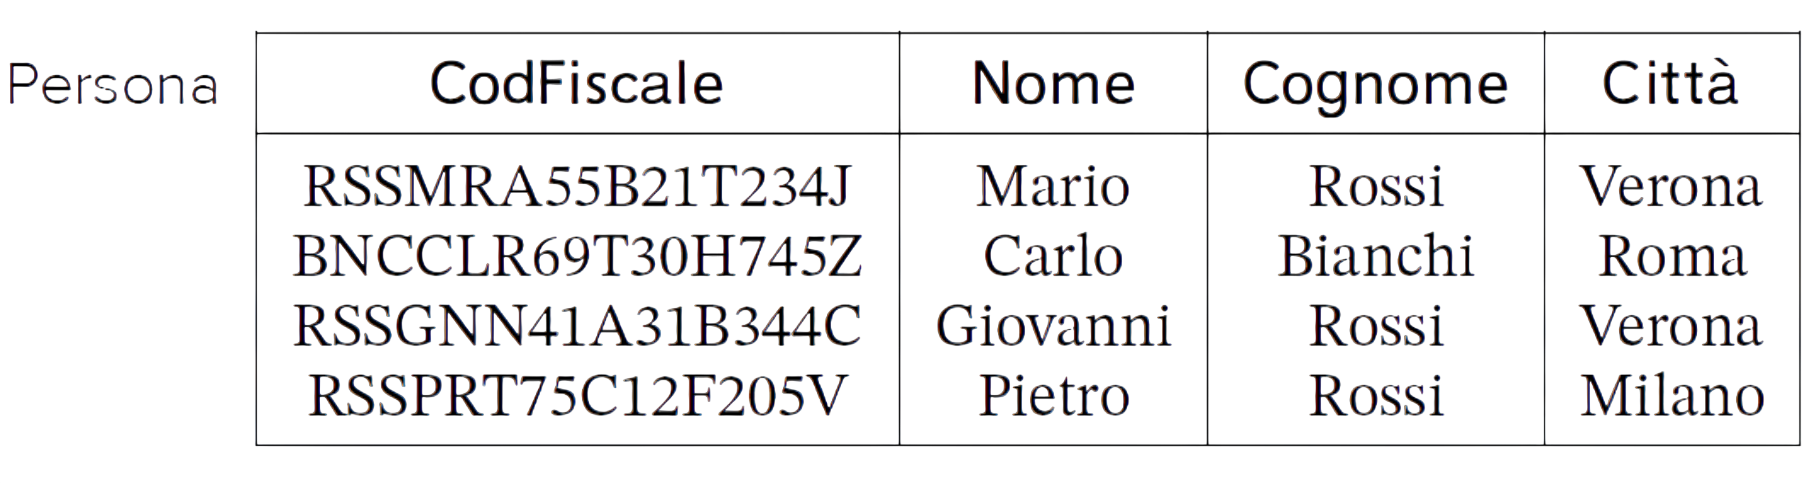
\includegraphics[width=0.6\textwidth]{images/tabella-persona.png}
  \end{center}

  \smallskip
  $\boldsymbol{\mathrm{Q_{10}}}$\textbf{: estrarre le città delle persone in cui il cognome è Rossi}
  \begin{lstlisting}[language=SQL]
  SELECT Citta
  FROM Persona
    WHERE Cognome = 'Rossi';
  \end{lstlisting}

  \smallskip
  L'output di questa interrogazione è la tabella:
  \begin{center}
    
\includegraphics[width=0.2\textwidth]{images/distinct-persona.png}
  \end{center}

  Per togliere i duplicati si può utilizzare la parola chiave $\verb|DISTINCT|$ dopo $\verb|SELECT|$:
  \begin{lstlisting}[language=SQL]
  SELECT DISTINCT Citta
  FROM Persona
    WHERE Cognome = 'Citta';
  \end{lstlisting}
  %foto
\end{esempiobox}

\section{Clausola \texttt{JOIN}}
In SQL, le interrogazioni con la clausola \verb|JOIN| si possono definire in due modi:
\begin{itemize}[label=$\triangleright$, itemsep=\smallskipamount]
  \item \textbf{senza l’uso di nuova sintassi}: specifica il legame tra le tabelle coinvolte a livello della clausola $\verb|WHERE|$
  \item \textbf{con l'uso di sintassi riservata} a livello di clausola $\verb|FROM|$
\end{itemize}

\smallskip
La clausola \verb|FROM| ammette come argomento:
\begin{lstlisting}[language=SQL]
  tabella [[AS] name] [, ...]
\end{lstlisting}

Si è visto che se sono presenti due o più nomi di tabelle, si esegue il prodotto cartesiano tra tutte le tabelle e lo schema del risultato
può contenere tutti gli attributi del prodotto cartesiano.\\[0.2ex]
Il prodotto cartesiano di due o più tabelle è un $\verb|CROSS JOIN|$.

\medskip
A partire da SQL-2, esistono altri tipi di \texttt{JOIN}:
\begin{itemize}[label=$\circ$, itemsep=\medskipamount]
  \item $\verb|INNER JOIN|$: restituisce solo le righe che soddisfano la condizione di join
  \item $\verb|LEFT [OUTER] JOIN|$: restituisce
  \begin{itemize}[label=$\diamond$, itemsep=\smallskipamount]
    \item tutte le righe della tabella di destra e sinistra che soddisfano la condizione di $\verb|join|$
    \item $\verb|null|$ per le righe della tabella di destra che non soddifisfano la condizione di di $\verb|join|$
  \end{itemize}
  \item $\verb|RIGH [OUTER] JOIN|$: restituisce
  \begin{itemize}[label=$\diamond$, itemsep=\smallskipamount]
    \item tutte le righe della tabella di destra e sinistra che soddisfano la condizione di $\verb|join|$
    \item $\verb|null|$ per le righe della tabella di sinistra che non soddifisfano la condizione di di $\verb|join|$
  \end{itemize}
  \item $\verb|FULL [OUTER] JOIN|$: restituisce
  \begin{itemize}[label=$\diamond$, itemsep=\smallskipamount]
    \item tutte le righe di entrambe le tabelle
    \item $\verb|null|$ per le righe che non soddifisfano la condizione di di $\verb|join|$
  \end{itemize}
\end{itemize}

In generale, la sintassi è:
\begin{lstlisting}[language=SQL]
tabella [NATURAL] join_type table_name [ ON condition [, ...]]
\end{lstlisting}

\begin{itemize}[label=$\triangleright$]
  \item $\verb|condition|$: espressione booleana che seleziona le tuple del $\verb|join|$ da aggiungere al risultato
\end{itemize}

\smallskip
Le tuple selezionate possono essere poi filtrate con la condizione della clausola $\verb|WHERE|$.

\begin{figure}[H]
  \centering
  \includegraphics[width=\textwidth]{images/Join.png}
\end{figure}

\subsection{Clausola \texttt{INNER JOIN}}
La sintassi è:
\begin{lstlisting}[language=SQL]
tabella [ INNER ] JOIN tabella ON join_condition [, ...]
\end{lstlisting}

Rappresenta il tradizionale $\theta$ $\verb|join|$ dell’algebra relazionale.\\[0.2ex]
Combina ciascuna riga $\mathrm{r_1}$ di $\mathrm{table_1}$ con ciascuna riga di $\mathrm{table_2}$ che soddisfa la condizione della clausola $\verb|ON|$.

\begin{esempiobox}{Interrogazione con \texttt{INNER JOIN}}
  \begin{lstlisting}[language=SQL]
  SELECT I.cognome, R.nomeRep, R.sede
  FROM Impiegato AS I
  INNER JOIN Reparto AS R ON I.nomeRep = R.nomeRep;
  \end{lstlisting}

  \begin{center}
    \includegraphics[width=0.5\textwidth]{images/tabellina.png}
  \end{center}
\end{esempiobox}

\subsection{Clausola \texttt{LEFT OUTER JOIN}}
La sintassi è:
\begin{lstlisting}[language=SQL]
tabella LEFT [ OUTER ] JOIN tabella ON join_condition [, ...]
\end{lstlisting}

Si esegue un $\verb|INNER JOIN|$.\\[0.2ex]
Poi, per ciascuna riga $\mathrm{r_1}$ di $\mathrm{table_1}$ che non soddisfa la condizione con qualsiasi riga di $\mathrm{table_2}$, si aggiunge una riga al risultato con i valori di $\mathrm{r_1}$ e assegnando $\verb|NULL|$ agli altri attributi.

\begin{esempiobox}{Interrogazione con \texttt{LEFT [OUTER] JOIN}}
  \begin{lstlisting}[language=SQL]
  INSERT INTO Reparto (nomerep, sede, telefono)
  VALUES ('Finanza', 'Padova', '02 8028888');

  SELECT R.nomeRep, I.cognome
  FROM Reparto AS R
  LEFT OUTER JOIN Impiegato AS I ON I.nomerep = R.nomerep;
  \end{lstlisting}

  \begin{center}
    \includegraphics[width=0.4\textwidth]{images/tabellina2.png}
  \end{center}
\end{esempiobox}

\vario{Nota}{
  Il $\texttt{LEFT OUTER JOIN}$ non è simmetrico!

  \smallskip
  Con le medisime tabelle si possono ottenere risultati diversi invertendo l’ordine delle tabelle nel join!
}

\subsection{Clausola \texttt{RIGHT OUTER JOIN}}
La sintassi è:
\begin{lstlisting}[language=SQL]
tabella RIGHT [ OUTER ] JOIN tabella ON join_condition [, ...]
\end{lstlisting}

\begin{esempiobox}{Interrogazione con \texttt{RIGHT [OUTER] JOIN}}
  \begin{lstlisting}[language=SQL]
  SELECT I.cognome , R.nomeRep
  FROM Impiegato I 
  RIGHT OUTER JOIN Reparto AS R ON I. nomerep = R. nomerep;
  \end{lstlisting}

  \begin{center}
    \includegraphics[width=0.5\textwidth]{images/tabellina2.png}
  \end{center}
\end{esempiobox}

\subsection{Clausola \texttt{FULL OUTER JOIN}}
La sintassi è:
\begin{lstlisting}[language=SQL]
tabella FULL [ OUTER ] JOIN tabella ON join_condition [, ...]
\end{lstlisting}

È equivalente a:
\begin{lstlisting}[language=SQL]
INNER JOIN + LEFT OUTER JOIN + RIGHT OUTER JOIN
\end{lstlisting}

Non è equivalente a $\verb|CROSS JOIN|$.

\section{Uso di variabili (alias)}
SQL permette di associare un nome alternativo (alias) alle tabelle che compaiono nella clausola $\verb|FROM|$.\\[0.2ex]
Il nome viene usato per far riferimento alla tabella nel contesto dell’interrogazione per diversi motivi:
\begin{itemize}[label=$\triangleright$, itemsep=\smallskipamount]
  \item far riferimento alla tabella in modo compatto
  \item fare accesso più volte alla stessa tabella
\end{itemize}

\begin{esempiobox}{Interrogazione con utilizzo di \texttt{AS}}
  Consideriamo la seguente tabella:

  \smallskip
  \begin{center}
    \includegraphics[width=0.6\textwidth]{images/tabella-impiegato.png  }
  \end{center}

  \smallskip
  $\boldsymbol{\mathrm{Q_{14}}}$\textbf{: estrarre tutti gli impiegati che hanno lo stesso cognome, ma nome diverso del dipartimento Produzione}
  \begin{lstlisting}[language=SQL]
  SELECT I1.Cognome, I2.Cognome
  FROM Impiegato I1, Impiegato I2
    WHERE I1.Cogmome = I2.Cognome AND
      I1.Nome <> I2.Cognome AND
      I2.Dipart = 'Produzione';
  \end{lstlisting}

  \smallskip
  Questa interrogazione confronta ciascuna riga di Impiegato con tutte le righe di Impiegato associate al dipartimento Produzione.

  \smallskip
  Si può immaginare che al momento della definizione dell’alias vengano create due copie della tabella Impiegato, ciascuna associata ad una delle due variabili $\mathrm{i_1}$ e $\mathrm{i_2}$.

  \smallskip
  Le due copie contengono tutte le righe di Impiegato.

  \smallskip
  Sulla copia $\mathrm{i_2}$ vengono selezionate solo le righe del dipartimento 'Produzione'.

  \smallskip
  \begin{center}
      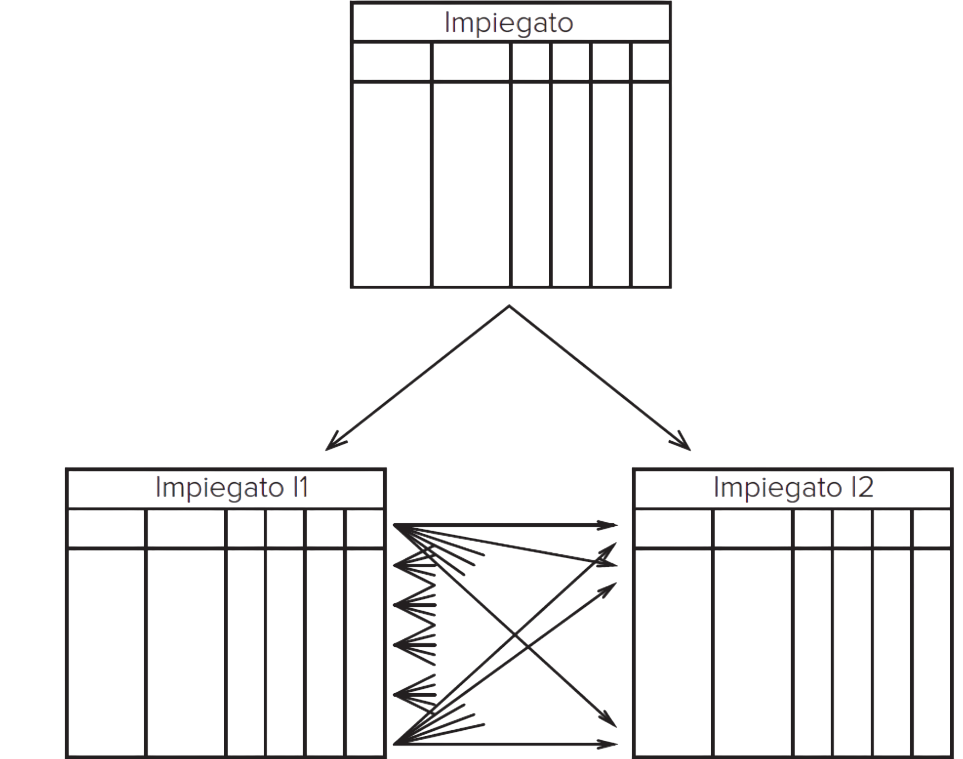
\includegraphics[width=0.4\textwidth]{images/Alias.png}
  \end{center}
\end{esempiobox}

\section{Clausola \texttt{ORDER BY}}
Una relazione è un insieme di tuple non ordinato, però, sorge spesso il bisogno di costruire un ordine sulle righe.\\[0.2ex]
SQL permette di specificare un ordinamento (ascendente o discendente) sulle righe dell‘output grazie alla clausola $\verb|ORDER BY|$ che chiude l‘interrogazione.

La sintassi è:
\begin{lstlisting}[language=SQL]
ORDER BY attributo [{ ASC | DESC }] [, ... ]
\end{lstlisting}

Le righe vengono ordinate per il primo attributo nell'elenco, a parità di valore del primo attributo si usa il secondo e così via in sequenza.

Di default l'ordinamento è $\verb|ASC|$.

\begin{esempiobox}{Interrogazione con \texttt{ORDER BY}}
  Consideriamo la seguente tabella:

  \smallskip
  \begin{center}
    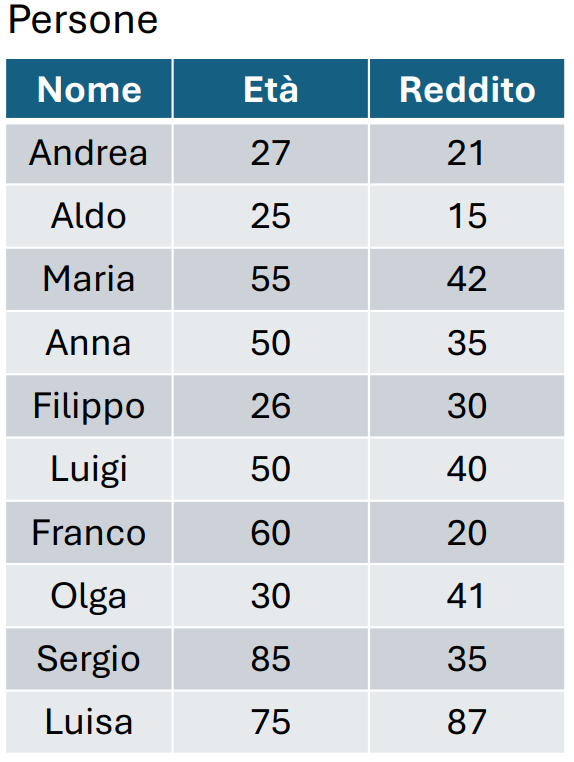
\includegraphics[width=0.3\textwidth]{images/tabella-persone.png}
  \end{center}

  \smallskip
  $\boldsymbol{\mathrm{Q_{15}}}$\textbf{: estrarre il nome, l'età e il reddito delle persone con meno di 30 anni in ordine alfabetico}

  \begin{lstlisting}[language=SQL]
  SELECT Nome, Eta, Reddito
  FROM Persone
    WHERE Eta < 30
      ORDER BY Eta;
  \end{lstlisting}
\end{esempiobox}

\begin{esempiobox}{Interrogazione con \texttt{ORDER BY}}
  Consideriamo la seguente tabella:

  \smallskip
  \begin{center}
    \includegraphics[width=0.5\textwidth]{images/Q11.png}
  \end{center}

  \smallskip
  $\boldsymbol{\mathrm{Q_{16}}}$\textbf{: estrarre il contenuto della tabella Automobile ordinato in base alla marca (discendente) e al modello}

  \begin{lstlisting}[language=SQL]
  SELECT *
  FROM Automobile
    ORDER BY Marca DESC, Modello;
  \end{lstlisting}
\end{esempiobox}

\section{Operazioni insiemistiche}
SQL mette a disposizione degli operatori insiemistci:
\begin{lstlisting}[language=SQL]
SELECT
  { UNION | INTERSECT | EXCEPT 
  [ALL] SELECT }
\end{lstlisting}

Gli operatori insiemistici, al contrario del resto del linguaggio, assumono come default di eseguire un'eliminazione dei duplicati, a meno che si usi $\verb|ALL|$.\\[0.2ex]
Sono sufficienti domini compatibili ed ugual numero di attributi.\\[0.2ex]
La corrispondenza si basa sulla posizione e se i nomi degli attributi sono diversi di solito il sistema usa il nome del primo operando.

\subsection{Unione}
\begin{esempiobox}{Interrogazione con unione}
  Consideriamo la seguente tabella:

  \smallskip
  \begin{center}
    \includegraphics[width=0.5\textwidth]{images/Q12.png}
  \end{center}

  \smallskip
  $\boldsymbol{\mathrm{Q}}$\textbf{: estrarre i nomi e i cognomi degli impiegati}

  \begin{lstlisting}[language=SQL]
  SELECT Nome
  FROM Impiegato
  UNION
  SELECT Cognome
  FROM Impiegato
  \end{lstlisting}
\end{esempiobox}

\begin{esempiobox}{Interrogazione con unione}
  Consideriamo la seguente tabella:

  \smallskip
  \begin{center}
    \includegraphics[width=0.5\textwidth]{images/Q13.png}
  \end{center}

  \smallskip
  $\boldsymbol{\mathrm{Q}}$\textbf{: etrarre i nomi e i cognomi degli impiegati eccetto quelli del dipartimento Amministrazione mantenendo i duplicati}

  \begin{lstlisting}[language=SQL]
  SELECT Nome
  FROM Impiegato
    WHERE Diaprt <> 'Amministrazione'
  UNION ALL
  SELECT Cognome
  FROM Impiegato
    WHERE Diaprt <> 'Amministrazione';
  \end{lstlisting}
\end{esempiobox}

\subsection{Intersezione}
\begin{esempiobox}{Interrogazione con intersezione}
  Consideriamo la seguente tabella:

  \smallskip
  \begin{center}
    \includegraphics[width=0.5\textwidth]{images/Q14.png}
  \end{center}

  \smallskip
  $\boldsymbol{\mathrm{Q}}$\textbf{: estrarre i cognomi degli impiegati che sono anche nomi}

  \begin{lstlisting}[language=SQL]
  SELECT Nome
  FROM Impiegato
  INTERSECT
  SELECT Cognome
  FROM Impiegato;
  \end{lstlisting}
\end{esempiobox}

\subsection{Differenza}
\begin{esempiobox}{Interrogazione con differenza}
  Consideriamo la seguente tabella:

  \smallskip
  \begin{center}
    \includegraphics[width=0.5\textwidth]{images/Q15.png}
  \end{center}

  \smallskip
  $\boldsymbol{\mathrm{Q}}$\textbf{: estrarre i nomi degli impiegati che non sono cognomi di qualche impiegato}

  \begin{lstlisting}[language=SQL]
  SELECT Nome
  FROM Impiegato
  EXCEPT
  SELECT Cognome
  FROM Impiegato;
  \end{lstlisting}
\end{esempiobox}

\section{Operatori aggregati}
Gli operatori di aggregazione permettono di valutare proprietà che dipendono da insiemi di tuple.

\subsection{Operatore \texttt{COUNT}}
L'operatore $\verb|COUNT|$ conta il numero di righe di una tabella o il numero di valori di uno o più attributi.

La sintassi è:
\begin{lstlisting}[language=SQL]
COUNT ( < * | [DISTINCT | ALL] ListaAttributi > )
\end{lstlisting}

\begin{itemize}[label=$\triangleright$, itemsep=\smallskipamount]
    \item $\verb|*|$: conta il numero di righe della tabella
    \item $\verb|DISTINCT ListaAttributi|$: conta il numero di valori diversi degli attributi ListaAttributi
    \item $\verb|ALL ListaAttributi|$: conta il numero di righe che hanno valori diversi da NULL negli attributi in ListaAttributi (default)
\end{itemize}

\begin{esempiobox}{Interrogazione con \texttt{COUNT}}
  Consideriamo la seguente tabella:

  \smallskip
  \begin{center}
    \includegraphics[width=0.5\textwidth]{images/Q16.png}
  \end{center}

  \smallskip
  $\boldsymbol{\mathrm{Q}}$\textbf{: estrarre il numero di impiegati del dipartimento di Produzione}
  \begin{lstlisting}[language=SQL]
  SELECT COUNT(*)
  FROM Impiegato
    WHERE Diaprt = 'Produzione';
  \end{lstlisting}
\end{esempiobox}

\begin{esempiobox}{Interrogazione con \texttt{COUNT}}
  Consideriamo la seguente tabella:

  \smallskip
  \begin{center}
    \includegraphics[width=0.5\textwidth]{images/Q17.png}
  \end{center}

  \smallskip
  $\boldsymbol{\mathrm{Q}}$\textbf{: estrarre il numero di valori diversi dell'attributo Stipendio fra tutte le righe di Impiegato}
  \begin{lstlisting}[language=SQL]
  SELECT COUNT(DISTINCT Stipendio)
  FROM Impiegato;
  \end{lstlisting}
\end{esempiobox}

\subsection{Operatore \texttt{SUM}}
L'operatore $\verb|SUM|$ estituisce la somma dei valori posseduti dall’espressione.

La sintassi è:
\begin{lstlisting}[language=SQL]
SUM ( < * | [DISTINCT | ALL] ListaAttributi > )
\end{lstlisting}

\begin{esempiobox}{Interrogazione con \texttt{SUM}}
  Consideriamo la seguente tabella:

  \smallskip
  \begin{center}
    \includegraphics[width=0.5\textwidth]{images/Q19.png}
  \end{center}

  \smallskip
  $\boldsymbol{\mathrm{Q}}$\textbf{: estrarre la somma degli stipendi del dipartimento Amministrazione}
  \begin{lstlisting}[language=SQL]
  SELECT SUM(Stipendio)
  FROM Impiegato
    WHERE Dipart = 'Amministrazione';
  \end{lstlisting}
\end{esempiobox}

\subsection{Operatore \texttt{MAX/MIN}}
Gli operatori $\verb|MIN|$ e $\verb|MAX|$ restituiscono rispettivamente il massimo e il minimo dei valori posseduti dall’espressione.

La sintassi è:
\begin{lstlisting}[language=SQL]
<MAX | MIN> ( [DISTINCT | ALL] ListaAttributi )
\end{lstlisting}

\subsection{Operatore \texttt{AVG}}
L'operatore $\verb|AVG|$ restiusce la media dei valori.

La sintassi è:
\begin{lstlisting}[language=SQL]
AVG ( [DISTINCT | ALL] ListaAttributi )
\end{lstlisting}

\begin{esempiobox}{Interrogazione con \texttt{MIN, MAX, AVG}}
  Consideriamo la seguente tabella:

  \smallskip
  \begin{center}
    \includegraphics[width=0.5\textwidth]{images/Q20.png}
  \end{center}

  \smallskip
  $\boldsymbol{\mathrm{Q}}$\textbf{: estrarre gli Stipendi minimi, massimi e medi fra quelli di tutti gli impiegati}
  \begin{lstlisting}[language=SQL]
  SELECT MIN(Stipendio), MAX(Stipendio), AVG(Stipendio)
  FROM Impiegato;
  \end{lstlisting}
\end{esempiobox}

\vario{Nota}{
  \begin{itemize}[label=$\triangleright$, itemsep=\smallskipamount]
  \item $\texttt{SUM}$ e $\texttt{AVG}$ ammettono come argomento solo espressioni che rappresentano valori numerici o intervalli di tempo
  \item $\texttt{MAX}$ e $\texttt{MIN}$ ammettono come argomento solo espressioni su cui è definito un ordinamento (quindi anche stringhe)
  \item $\texttt{DISTINCT}$ elimina i duplicati
  \item $\texttt{ALL}$ trascura solo i valori nulli
\end{itemize}
}

\begin{esempiobox}{ATTENZIONE}
  \begin{lstlisting}[language=SQL]
  SELECT Cognone, Nome, MAX(I.Stipendio)
  FROM Impiegato AS I
  JOIN Diparmento AS D ON I.Dipart = D.Nome
    WHERE D.Citta = 'Milano';
  \end{lstlisting}

  \textcolor{black!60!red}{\textbf{La seguente interrogazione non è corretta!}}
  
  \smallskip
  Gli operatori aggregati non sono un meccanismo di selezione, ma solo funzioni che restituiscono un valore quando sono applicate ad un insieme.

  \smallskip
  Cognome e Nome restituiscono un valore per ogni tupla selezionata, mentre $\texttt{MAX}$ restituisce un valore unico per tutto l’insieme.

  \smallskip
  Per risolvere questa situazione serve il meccanismo di \textbf{raggruppamento}.
\end{esempiobox}


\section{Clausola \texttt{GROUP BY}}
Gli operatori aggregate possono essere applicati separatamente a sottoinsiemi di righe.\\[0.2ex]
La clausola $\verb|GROUP BY|$ permette di specificare come dividere le tabelle in sottoinsiemi.\\[0.2ex]
La clausola permette di specificare un insieme di attributi e l’interrogazione raggrupperà le righe che possiedono gli stessi valori per questo insieme di attributi.

\begin{esempiobox}{Interrogazione con \texttt{GROUP BY}}
Consideriamo la seguente tabella:

\smallskip
\begin{center}
  \includegraphics[width=0.5\textwidth]{images/Q22.png}
\end{center}

\smallskip
$\boldsymbol{\mathrm{Q}}$\textbf{: estrarre la somma degli stipendi di tutti gli impiegati dallo stesso dipartimento}
\begin{lstlisting}[language=SQL]
SELECT Dipart, SUM(Stipendio)
FROM Impiegato
  GROUP BY Diaprt;
\end{lstlisting}
\end{esempiobox}

\smallskip
In una interrogazione che fa uso della clausola $\verb|GROUP BY|$ può comparire come argomento della $\verb|SELECT|$ solo un sottoinsieme degli attributi usati nella clausola $\verb|GROUP BY|$, oppure, operatori di aggregazione.

\subsection{Clausola \texttt{HAVING}}
È possibile applicare delle selezioni ai gruppi generati tramite la clausola $\verb|GROUP BY|$.\\[0.2ex]
La clausola $\verb|HAVING|$ permette di specificare delle condizioni che devono essere soddisfatte dai gruppi generati dopo l’esecuzione del raggruppamento tramite $\verb|GROUP BY|$.

La sintassi è:
\begin{lstlisting}[language=SQL]
SELECT Dipart, SUM(Stipendio) AS SommaStipendi
FROM Impiegato
  GROUP BY Dipart
    HAVING SUM(Stipendio) > 100;
\end{lstlisting}

Dopo aver eseguito i raggruppamenti, vengono mantenuti solo i gruppi che soddisfano la condizione specificata nella clausola $\verb|HAVING|$.

\begin{figure}[H]
\centering
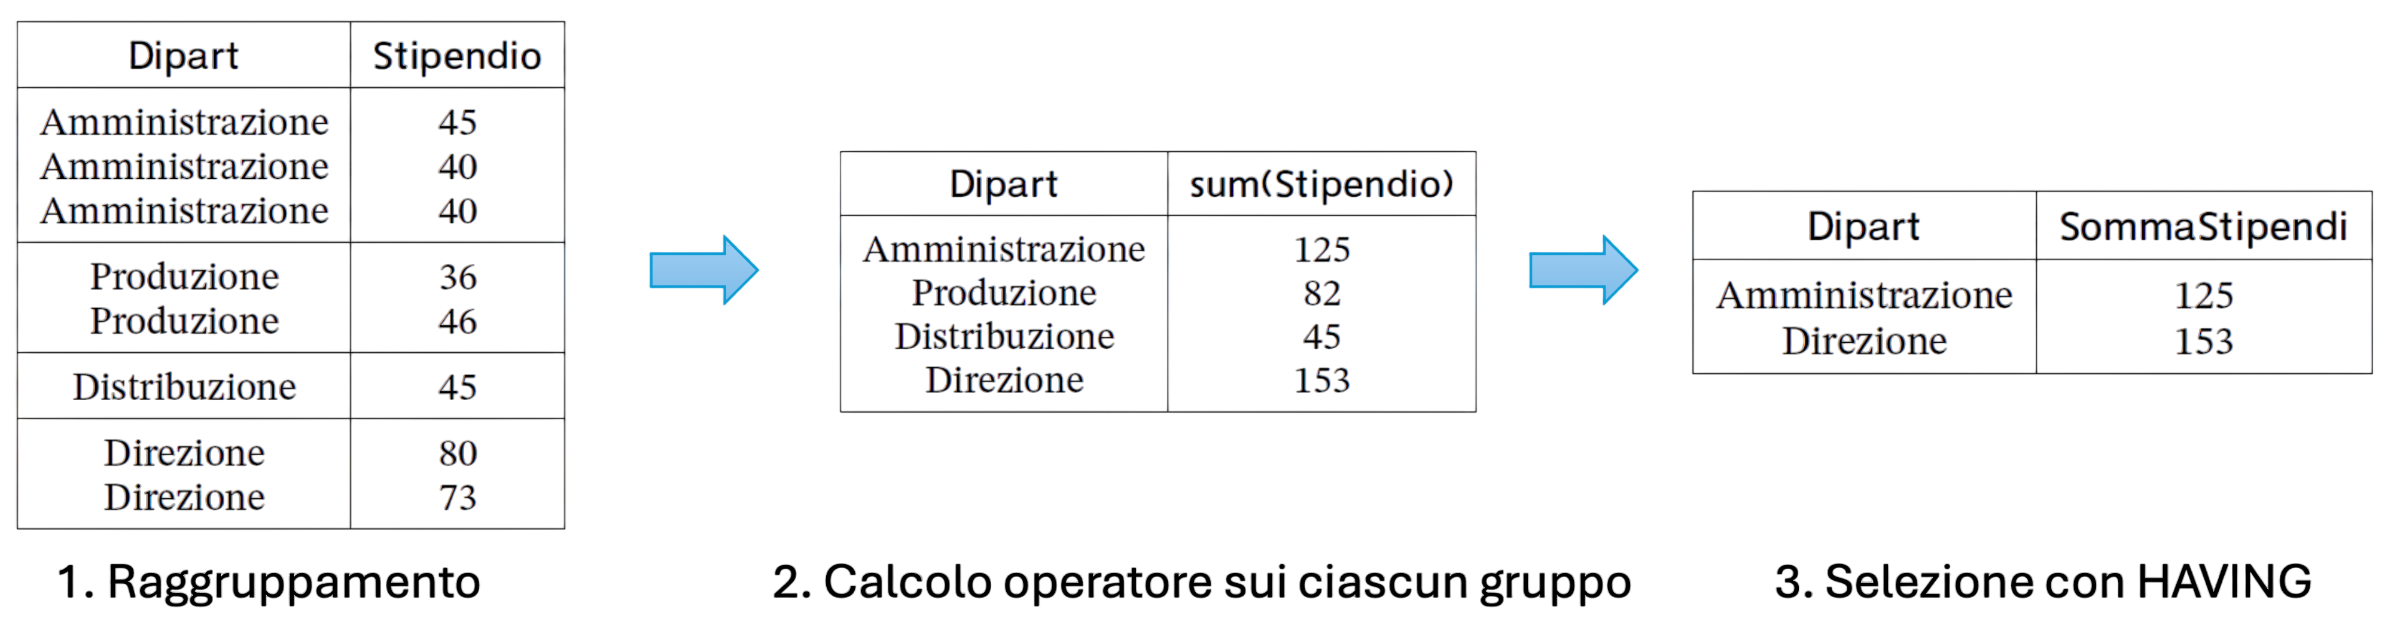
\includegraphics[width=\textwidth]{images/esempio.png}
\end{figure}

\begin{esempiobox}{OSSERVAZIONE}
\begin{itemize}[label=$\triangleright$, itemsep=\smallskipamount]
  \item clausola $\texttt{WHERE}$ applica delle selezioni su singole righe, \textcolor{purple}{\textbf{prima}} dell’eventuale raggruppamento tramite $\texttt{GROUP BY}$
  \item clausola $\texttt{HAVING}$ applica delle selezioni su gruppi, generati a \textcolor{purple}{\textbf{seguito}} dell’esecuzione del raggruppamento tramite $\texttt{GROUP BY}$
\end{itemize}

\begin{lstlisting}[language=SQL]
SELECT Dipart
FROM Impiegato
  WHERE Ufficio = 20 -- seleziona righe raggruppate
    GROUP BY Dipart  -- forma gruppi con righe selezionate
      HAVING AVG(Stipendio) > 25; -- seleziona gruppi del risultato
  \end{lstlisting}
\end{esempiobox}

\section{Interrogazioni nidificate}
Un' interrogazione nidificata è un'interrogazione che contiene al suo interno altre interrogazioni.\\[0.2ex]
La nidificazione può avvenire sia nella clausola $\verb|SELECT|$, che nella clausola $\verb|FROM|$, che nella clausola $\verb|WHERE|$.\\[0.2ex]
Il caso tipico è la nidificazione nella clausola $\verb|WHERE|$, dove un predicato contiene un confronto tra un valore (espressione su una singola riga) ed il risultato di un’interrogazione SQL.

\subsection{Clausola \texttt{WHERE}}
Se in un predicato si confronta un attributo o una espressione che produce un valore singolo con il risultato di un’interrogazione, sorge il problema di disomogeneità dei termini del confronto.\\[0.2ex]
I normali operatori di confronto ($\verb|=|, \verb|<>|, \verb|<|, \verb|>|, \verb|<=|, \verb|=>|$) possono essere estesi con le parole chiave $\verb|ANY|$ e $\verb|ALL|$:
\begin{itemize}[label=$\triangleright$, itemsep=\smallskipamount]
\item $\verb|ANY|$: riga soddisfa la condizione se risulta vero il confronto (con l’operatore specificato) tra il valore dell’attributo (o espressione) e \textbf{almeno} uno degli elementi restituiti dall’interrogazione 
\item $\verb|ALL|$: riga soddisfa la condizione se risulta vero il confronto (con l’operatore specificato) tra il valore dell’attributo (o espression) e \textbf{tutti} gli elementi restituiti dall’interrogazione
\end{itemize}

\begin{esempiobox}{Interrogazione con \texttt{WHERE}}
Consideriamo la seguente tabella:

\smallskip
\begin{center}
  \includegraphics[width=0.5\textwidth]{images/Q24.png}
\end{center}

\smallskip
$\boldsymbol{\mathrm{Q}}$\textbf{: estrarre i dipartimenti in cui non lavorano persone di cognome Rossi}
\begin{lstlisting}[language=SQL]
SELCET Nome
FROM Diparmento
  WHERE Nome <> ALL (
    SELECT Dipart
    FROM Impiegato
      WHERE Cognome = 'Rossi'
  );
\end{lstlisting}

\smallskip
Questo equivale a:
\begin{lstlisting}[language=SQL]
SELECT Nome
FROM Dipartimento
EXCEPT
SELECT Dipart
FROM Impiegato
WHERE Cognome = 'Rossi';
\end{lstlisting}
\end{esempiobox}

\vario{ATTENZIONE!}{
Per le interrogazioni nidificate viste fino ad ora, l’interrogazione può essere eseguita una volta sola ed il risultato ottenuto può essere salvato in una tabella temporanea usata per eseguire ciascun confronto con le righe dalla tabella esterna.

\smallskip
Talvolta però l’interrogazione nidificata fa riferimento al contesto dell’interrogazione che la racchiude attraverso l’uso di una variabile (\textbf{passaggio di binding}).

\smallskip
L’interrogazione nidificata dovrà essere \textbf{valutata separatamente per ciascuna riga} prodotta dalla valutazione della query esterna.
}

\subsection{Clausola \texttt{EXISTS}}
L'operatore logico $\verb|EXISTS|$ riceve come parametro un'interrogazione nidificata e restituisce il valore vero solo se l'interrogazione fornisce un risultato non vuoto.\\[0.2ex]
Questo operatore può essere usato in modo significativo soloquando si ha un passaggio di binding tra la query esterna e quella interna.

\begin{esempiobox}{Interrogazione con \texttt{EXISTS}}
Consideriamo la seguente tabella:

\smallskip
\begin{center}
  \includegraphics[width=0.5\textwidth]{images/Q25.png}
\end{center}

\smallskip
$\boldsymbol{\mathrm{Q}}$\textbf{: estrarre le persone che hanno degli omonimi (stesso nome e cognome, ma codice fiscale diverso)}
\begin{lstlisting}[language=SQL]
SELECT *
FROM Persona AS P
  WHERE EXISTS (
    SELECT *
    FROM Persona P1
    WHERE P1.Nome = P.Nome AND
      P1.Cognome = P.Cognome AND
      P1.CodFiscale <> P.CodFiscale
  );
\end{lstlisting}
\end{esempiobox}

\subsection{Clausola \texttt{SELECT}}
Le interrogazioni nidificate possono essere specificate anche come elemento della clausola $\verb|SELECT|$.

\vario{Nota}{
  Spesso l'uso di query nidificate nella \texttt{SELECT} sostituiscono l'uso del \texttt{JOIN}.
}

\begin{esempiobox}{Interrogazione con \texttt{SELECT}}
Consideriamo la seguente tabella:

\smallskip
\begin{center}
    \includegraphics[width=0.5\textwidth]{images/Q27.png}
\end{center}

\smallskip
$\boldsymbol{\mathrm{Q}}$\textbf{: estrarre per ogni cantante il numero di canzoni di cui è autore}
\begin{lstlisting}[language=SQL]
  SELECT DISTINCT Nome, NumCanzoni = (
    SELECT COUNT(*)
    FROM Autore AS A
      WHERE A.Nome = C.Nome
  )
  FROM Cantante AS C;
\end{lstlisting}
\end{esempiobox}


\subsection{Clausola \texttt{FROM}}
Le interrogazioni nidificate possono essere utilizzate nella clausola $\verb|FROM|$ come sorgente dati su cui eseguire l’interrogazione.\\[0.2ex]
È possibile creare una catena di interrogazioni, dove ciascuna interrogazione utilizza il risultato della precedente come una tabella di base.

\begin{esempiobox}{Interrogazione con \texttt{FROM}}
Consideriamo la seguente tabella:

\smallskip
\begin{center}
    \includegraphics[width=0.5\textwidth]{images/Q28.png}
\end{center}

\smallskip
$\boldsymbol{\mathrm{Q}}$\textbf{: estrarre per ogni cantante che è anche autore di canzoni il numero di canzoni di cui è rispettivamente interprete e autore}
\begin{lstlisting}[language=SQL]
SELECT DISTINCT C.Nome, C.NumCantate, A.NumScritte
FROM (
  SELECT Nome, COUNT(*) AS NumCantate
  FROM Cantante
) AS C
JOIN (
  SELECT Nome, COUNT(*) AS NumScritte
  FROM Autore
) AS A ON C.Nome = A.Nome;
\end{lstlisting}
\end{esempiobox}
    
    %!TeX root = BasiDiDati.tex

\chapter{Strutture fisiche e di accesso ai dati}
Le basi di dati risiedono nella \textcolor{azzurrino}{\textbf{memoria secondaria}} perchè sono:
\begin{itemize}[label=$\triangleright$, itemsep=\smallskipamount]
  \item \textbf{grandi}: non possono essere contenute completamente in memoria centrale
  \smallskip
  \item \textbf{persistenti}: hanno un tempo di vita che non è limitato all'esecuzione dei programmi che le usano
\end{itemize}

\vario{Caratteristiche della memoria secondaria}{
  Le caratteristiche principali della memoria secondaria sono:
  \begin{itemize}[label=$\circ$, itemsep=\smallskipamount]
    \item \textbf{non utilizzabile direttamente dai programmi}
    \item \textbf{dati organizzati in blocchi} (grandezza dipende dal sistema operativo)
    \item \textbf{operazioni possibili}:
    \begin{itemize}[label=$\diamond$]
      \item lettura intero blocco
      \item scrittura intero blocco
    \end{itemize}
    \item \textbf{costo delle operazioni di accesso alla memoria secondaria è maggiore al costo per accedere ai dati in memoria centrale}
  \end{itemize}
}

\section{Gestore del buffer}
L'interazione tra memoria secondaria e memoria centrale avviene tramite il \textcolor{azzurrino}{\textbf{gestore del buffer}}, mediante il trasferimento di uno o più \textbf{blocchi} della memoria secondaria in \textbf{pagine} dedicate della memoria centrale (buffer).

\vario{Precisazione}{
  La dimensione delle pagine in memoria centrale sono solitamente un multiplo della dimensione dei blocchi in memoria secondaria.

  \smallskip
  Per semplificare, si assume che siano uguali:
  \begin{equation*}
    \text{1 pagina} \approx \text{1 blocco}
  \end{equation*}
}

\subsection{Buffer}
Il \textcolor{azzurrino}{\textbf{buffer}} è una zona della memoria condivisa dalle applicazioni e una gestione ottimale del buffer consente di ottenere buone prestazioni nell'accesso ai dati.\\[0.2ex]
Quando uno stesso dato viene utilizzato più volte in tempi ravvicinati il buffer evita
l'accesso alla memoria secondaria.

\vario{Compito del gestore del buffer}{
  Il gestore del buffer si occupa di caricare e salvare i dati dalla memoria secondaria alla memoria centrale.
}

\subsection{Politica di gestione della memoria}
L'obiettivo del gestore del buffer è di \hl{ottimizzare gli accessi} attraverso le politiche di gestione della memoria:
\begin{itemize}[label=$\diamond$, itemsep=\bigskipamount]
  \item \textbf{lettura di un blocco}:
  \begin{itemize}[label=$\triangleright$, itemsep=\medskipamount]
    \item blocco presente in una pagina del buffer
    \begin{itemize}[label=$\Rightarrow$, itemsep=\smallskipamount]
      \item non viene eseguita la lettura in memoria secondaria
      \item viene restituito un puntatore alla pagina del buffer
    \end{itemize}
    \item blocco non presente in una pagina del buffer
    \begin{itemize}[label=$\Rightarrow$, itemsep=\smallskipamount]
      \item viene cercata una pagina libera
      \item viene caricato il blocco nella pagina
      \item viene restituito il puntatore alla pagina del buffer
    \end{itemize}
  \end{itemize}
  \item \textbf{scrittura di un blocco}: se viene effettuata una richiesta si scrittura di un blocco già caricato in una pagina del buffer, il gestore del buffer può decidere di \hl{differire la scrittura} su memoria secondaria in un secondo momento
\end{itemize}

\medskip
Per poter aumentare la velocità di accesso ai dati, le politiche di lettura e scrittura si basano sul \textbf{principio di località}.

\definizione{principio di località}{
  Il \textbf{principio di località} si basa sul fatto che i dati referenziati di recente hanno maggiore probabilità di essere referenziati nuovamente in futuro.
}

\subsection{Gestione delle pagine}
Il contenuto del buffer lo possiamo immaginare come una matrice.

\begin{figure}[H]
  \centering
  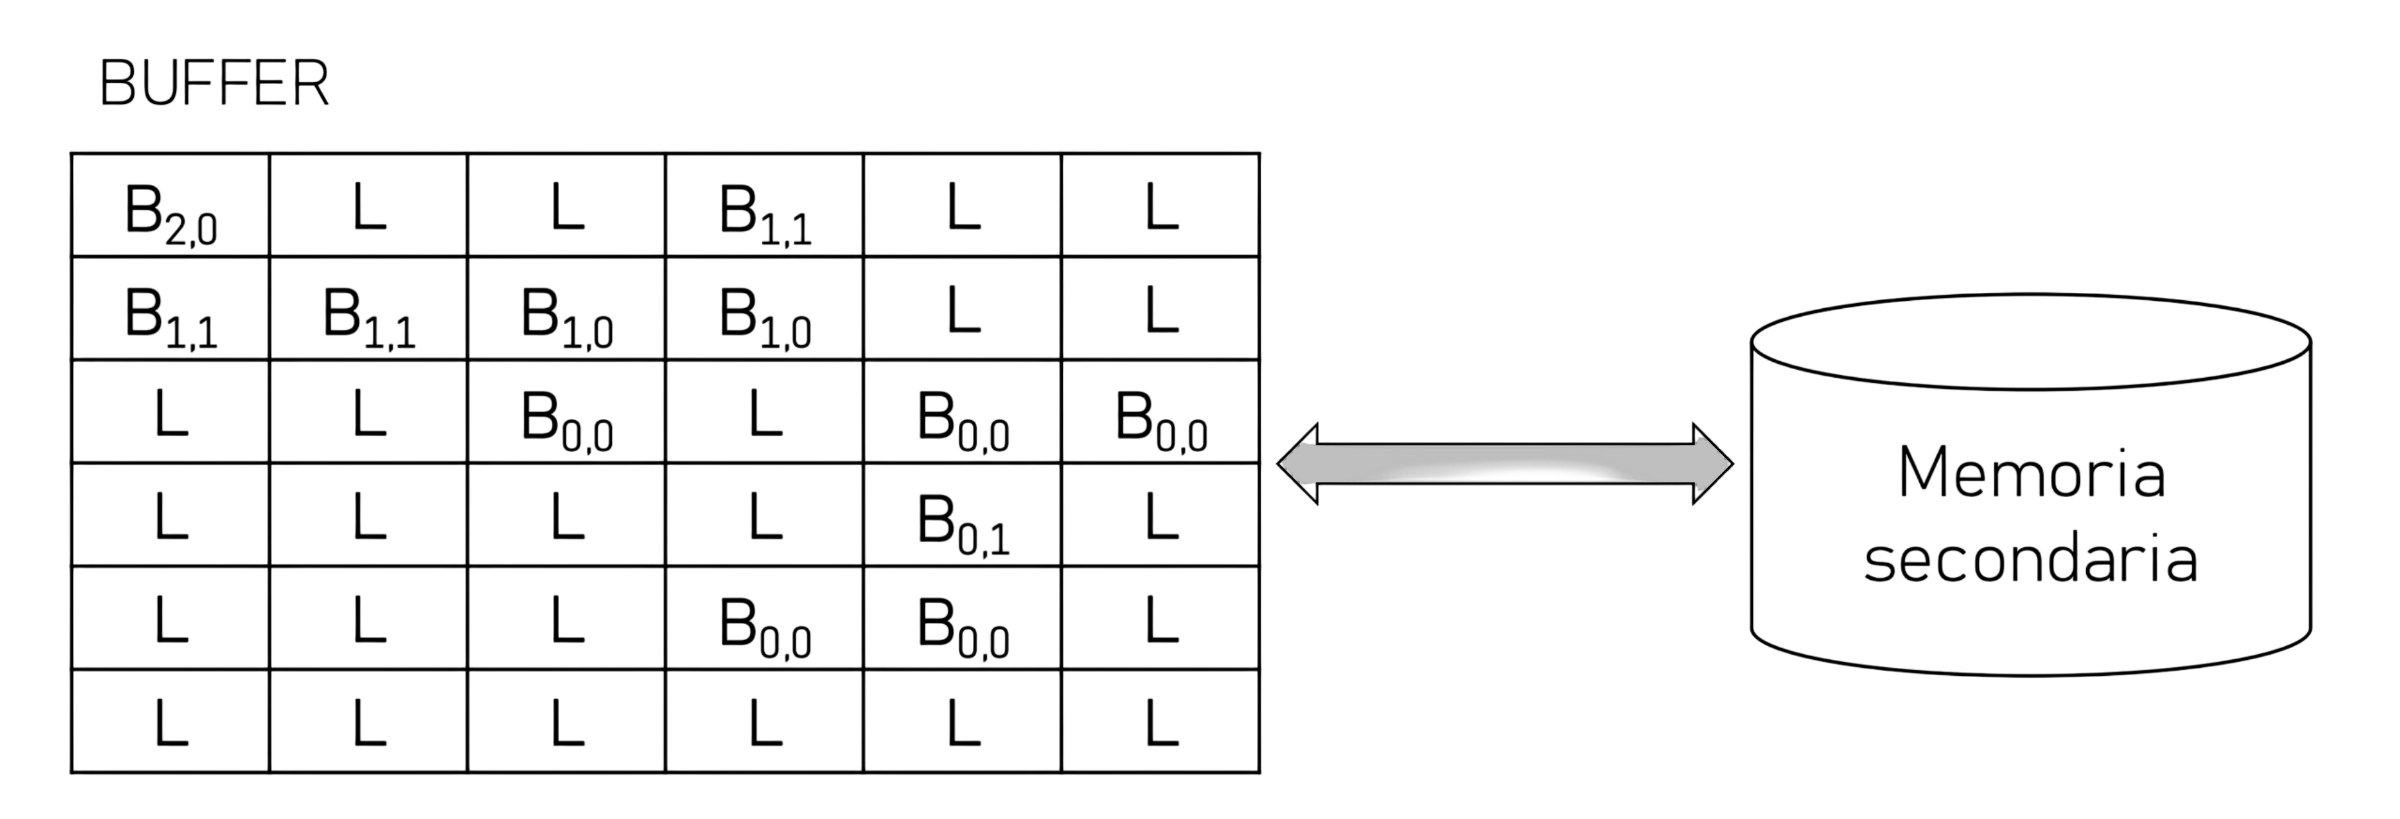
\includegraphics[width=0.6\textwidth]{images/gestione-pagine.png}
\end{figure}

Per ogni pagina del buffer si memorizza:
\begin{itemize}[label=$\triangleright$, itemsep=\smallskipamount]
  \item \textbf{blocco B} (L se libero) indicando il file e il numero di blocco (offset)
  \item \textbf{variabili di stato} ($\mathrm{B_{i,j}}$):
  \begin{itemize}[label=$\circ$, itemsep=\smallskipamount]
    \item \textbf{contatore} $\mathbf{i}$: indica il numero di transazioni
    \item \textbf{bit di stato} $\mathbf{j}$: indica se la pagina è stata modificata (1) o no (0)
  \end{itemize}
\end{itemize}

\subsection{Primitive per la gestione del buffer}

\subsubsection{Primitiva \protect\texttt{fix}}
La \textcolor{azzurrino}{primitiva \texttt{fix}} viene utilizzata dalle transazioni per richiedere l'accesso a un blocco e restituisce un puntatore alla pagina contente il blocco richiesto.

Le azioni della primitiva sono:
\begin{itemize}[label=$\triangleright$, itemsep=\medskipamount]
  \item \textbf{ricerca del blocco}:
  \begin{itemize}[label=$\diamond$, itemsep=\medskipamount]
    \item blocco viene trovato
    \begin{itemize}[label=$\Rightarrow$, itemsep=\smallskipamount]
      \item viene restituito un puntatore alla pagina contentente il blocco
    \end{itemize}
    \item blocco non viene trovato:
    \begin{itemize}[label=$\circ$, itemsep=\smallskipamount]
      \item viene scelta una pagina libera
      \begin{itemize}[label=$\Rightarrow$, itemsep=\smallskipamount]
        \item viene salvata in memoria secondaria (primitiva $\verb|flush|$)
        \item viene caricato il blocco in P aggiornando file e numero di blocco
      \end{itemize}
      \item non ci sono pagine libere
      \begin{itemize}[label=$\Rightarrow$, itemsep=\smallskipamount]
        \item viene rubata una pagina a un'altra transazione (primitiva $\verb|flush|$)
        \item viene sospesa la transazione inserendola in una coda di attesa
        \item se si libera una pagina il gestore si comporterà come al punto precedente
      \end{itemize}
    \end{itemize}
  \end{itemize}
\end{itemize}
\medskip
\begin{itemize}[label=$\Rightarrow$]
  \item \textcolor{red}{\textbf{effetto della modifica}}: quando una transizione accede a una pagina per la prima volta il contatore si incrementa
\end{itemize}

\subsubsection{Primitiva \protect\texttt{unfix}}
La \textcolor{azzurrino}{primitiva \texttt{unfix}} viene usata dalle transazioni per indicare che la transazione ha terminato di usare il blocco.

\begin{itemize}[label=$\Rightarrow$]
  \item \textcolor{red}{\textbf{effetto della modifica}}: decremento del contatore $\mathrm{i}$
\end{itemize}

\subsubsection{Primitiva \protect\texttt{setDirty}}
La \textcolor{azzurrino}{primitiva \texttt{setDirty}} viene utilizzata dalle transazioni per indicare al gestore del buffer che il blocco della pagina è stato modificato.

\begin{itemize}[label=$\Rightarrow$]
  \item \textcolor{red}{\textbf{effetto della modifica}}: bit di stato $\mathrm{j}$ passa da 0 a 1
\end{itemize}

\subsubsection{Primitiva \protect\texttt{force}}
La \textcolor{azzurrino}{primitiva \texttt{force}} viene utilizzata per salvare in memoria secondaria in \hl{modo sincrono} il blocco contenuto nella pagina.\\[0.2ex]
Questa primitiva viene usata dal gestore dell'affidabilità.

\begin{itemize}[label=$\Rightarrow$]
  \item \textcolor{red}{\textbf{effetto della modifica}}: viene salvato in memoria secondaria il blocco e il bit di stato $\mathrm{j}$ posto a 0
\end{itemize}

\subsubsection{Primitiva \protect\texttt{flush}}
La \textcolor{azzurrino}{primitiva \texttt{flush}} viene utilizzata per salvare i blocchi in memoria secondaria in \hl{modo asincrono}.\\[0.2ex]
Questa primitiva viene usata dal gestore del buffer.

\begin{itemize}[label=$\Rightarrow$]
  \item \textcolor{red}{\textbf{effetto della modifica}}: viene liberata la pagina "dirty" e il bit di stato $\mathrm{j}$ viene posto a 0
\end{itemize}

\section{Gestore dell'affidabilità}
Il gestore del buffer differisce le operazioni di scrittura e questo potrebbe rappresentare un pericolo.\\[0.2ex]
Il \textcolor{azzurrino}{\textbf{gestore dell'affibilità}} si occupa di garantire:
\begin{itemize}[label=$\triangleright$, itemsep=\smallskipamount]
  \item \textbf{atomicità}: transazioni non devono essere incomplete
  \item \textbf{persistenza}: effetti di ciascuna transazione non conclusa con un commit devono essere mantenuti in modo permanente
\end{itemize}

\begin{figure}[H]
  \centering
  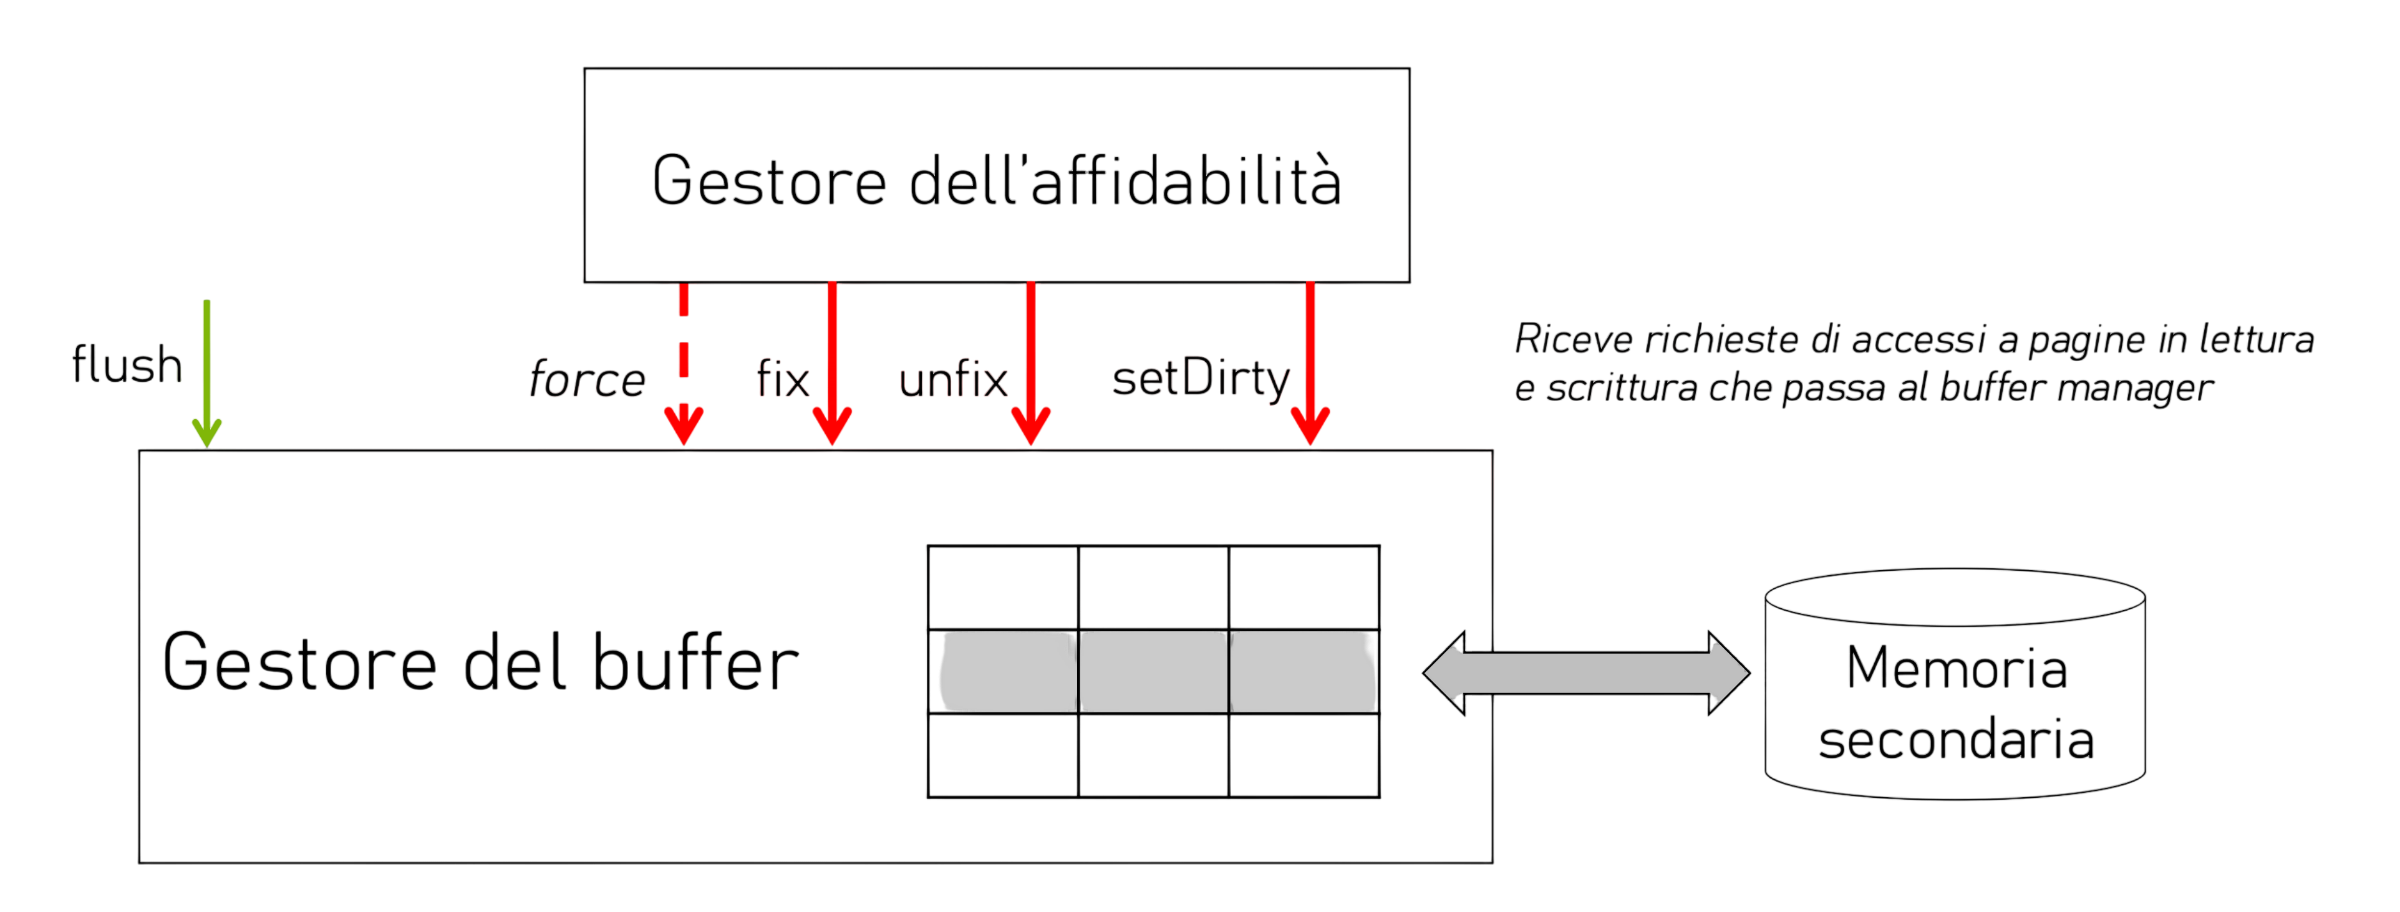
\includegraphics[width=0.6\textwidth]{images/gestore-affidabilità.png}
\end{figure}


\subsection{File di LOG}
Il funzionamento del gestore dell'affidabilità si basa sull'utilizzo del \textbf{file di LOG}.

\definizione{file di LOG}{
  Il \textbf{file di LOG} è un archivio persistente su cui vengono registrate tutte le operazioni eseguite dal DBMS.
}

Per il corretto funzionamento, il gestore dell'affidabilità deve disporre di un dispositivo di \textbf{memoria stabile} (resistente ai guasti).

Il file di LOG viene memorizzato in memoria stabile e al suo interno vengono memorizzati:
\begin{itemize}[label=$\triangleright$, itemsep=\medskipamount]
  \item \textbf{record di transizione}: record che descrivono informazioni sulle transazioni
  \begin{itemize}[label=$\diamond$, itemsep=\smallskipamount]
    \item $\mathbf{B(T)}$: \textcolor{azzurrino}{\textbf{begin}} della transazione
    \item $\mathbf{C(T)}$: \textcolor{azzurrino}{\textbf{commit}} della transazione
    \item $\mathbf{A(T)}$: \textcolor{azzurrino}{\textbf{abort}} della transazione
    \item $\mathbf{I(T,O,AS)}$: \textcolor{azzurrino}{\textbf{insert}} di un oggetto $\mathrm{O}$ da parte di una transazione $\mathrm{T}$ con il suo after state $\mathrm{AS}$ (stato dell'oggetto dopo l'operazione)
    \item $\mathbf{D(T,O,AS)}$: \textcolor{azzurrino}{\textbf{delete}} di un oggetto $\mathrm{O}$ da parte della transizione $\mathrm{T}$ con il suo before state $\mathrm{BS}$ (stato dell'oggetto prima dell'operazione)
    \item $\mathbf{U(T,O,BS,AS)}$: \textcolor{azzurrino}{\textbf{update}} di un oggetto $\mathrm{O}$ da parte della transizione $\mathrm{T}$ con il suo before state $\mathrm{BS}$ e il suo after state $\mathrm{AS}$
  \end{itemize}
  \item \textbf{record di sistema}: record che descrivono informazioni sulle operazioni esaguite dal DBMS
  \begin{itemize}[label=$\circ$, itemsep=\smallskipamount]
    \item $\mathbf{DUMP}$: copia completa e consistente della base di dati.
    \item $\mathbf{CK(T_1, \dots, T_n)}$: indica che all'esecuzione del checkpoint, le transazioni attive erano $\mathrm{T_1, \dots, T_n}$
    \begin{itemize}[itemsep=\smallskipamount]
      \item elenco delle transazioni che non hanno ancora espresso la loro scelta relativamente all'esito finale
      \item operazione svolta periodicamente affinché i dati delle transazioni che hanno eseguito il \texttt{commit} siano registrati in modo permanente
      \item il protocollo di checkpoint prevede i seguenti passi:
      \begin{enumerate}[itemsep=\smallskipamount]
        \item sospensione delle operazioni di \texttt{scrittura}, \texttt{commit} e \texttt{abort} delle transazioni
        \item esecuzione della primitiva \texttt{force} sulle pagine ``dirty'' di transazioni che hanno eseguito il \texttt{commit}
        \item scrittura sincrona (primitiva \texttt{force}) sul file di LOG del record di checkpoint con gli identificatori delle transazioni attive
        \item ripresa delle operazioni di \texttt{scrittura}, \texttt{commit} e \texttt{abort} delle transazioni
      \end{enumerate}
    \end{itemize}
  \end{itemize}
\end{itemize}

I record di transazione salvati nel LOG consentono di eseguire in caso di ripristino le seguenti operazioni:
\begin{itemize}[label=$\triangleright$, itemsep=\smallskipamount]
  \item $\mathbf{UNDO}$: viene usato per disfare un'azione su un oggetto $\mathrm{O}$.
  
  \hl{È sufficiente ricopiare in $\mathrm{O}$ il valore d $\mathrm{BS}$}.
  
  L'\texttt{insert}/\texttt{delete} viene disfatto cancellando/inserendo $\mathrm{O}$
  \item $\mathbf{REDO}$: serve per rifare un'azione su un oggetto $\mathrm{O}$.
  
  \hl{È sufficiente ricopiare in $\mathrm{O}$ il valore $\mathrm{AS}$}.
  
  L'\texttt{insert}/\texttt{delete} viene rifatto inserendo/cancellando $\mathrm{O}$
\end{itemize}

\medskip
Gli inserimenti controllano sempre l’esistenza di $\mathrm{O}$ prima di eseguire l'operazione.\\[0.2ex]
Per queste operazioni vale la \textbf{proprietà di idempotenza}.

\definizione{proprietà di idempotenza}{
  \[
    \begin{aligned}
      \mathrm{UNDO(UNDO(A))} &= \mathrm{UNDO(A)}\\
      \mathrm{REDO(REDO(A))} &= \mathrm{REDO(A)}
    \end{aligned}
  \]
}

\subsection{Regole di scrittura sul file di LOG}
Il gestore dell'affidabilità deve rispettare le seguenti regole di scrittura sul file di LOG:
\begin{itemize}[label=$\Rightarrow$, itemsep=\smallskipamount]
  \item \textbf{regola Write Ahead Logging}: record di LOG devono essere scritti sul LOG precedente all'esecuzione delle corrispondenti operazioni sulla base di dati (garantisce la possibilità di fare sempre \texttt{UNDO})
  \item \textbf{regola di commit-precedenza}: record di LOG devono essere scritti sul LOG prima dell'esecuzione del \texttt{commit} della transazione (garantisce la possibilità di fare sempre \texttt{REDO})
\end{itemize}

Queste regole consentono di salvare i blocchi delle pagine “dirty” in modo totalmente asincrono rispetto al commit delle transazioni.

\subsection{Guasti}
Una transazione $\mathrm{T}$ sceglie in modo atomico l'esito di $\verb|commit|$ nel momento in cui scrive nel file di LOG in modo sincrono (primitiva $\verb|force|$) il suo record di $\verb|commit| \ \mathrm{C(T)}$. 

\begin{itemize}[label=$\Rightarrow$, itemsep=\smallskipamount]
  \item se avviene un guasto prima della scrittura del record di $\verb|commit|$ $\rightarrow$ $\mathbf{UNDO}$
  \item se avviene un guasto dopo la scrittura del record di $\verb|commit|$ $\rightarrow$ $\mathbf{REDO}$
\end{itemize}

Esistono due tipologie di guasto:
\begin{itemize}[label=$\triangleright$, itemsep=\medskipamount]
  \item \textbf{guasto di sistema}: perdita del contenuto della memoria centrale.
  
  Viene risolto con la tecnica della \textcolor{azzurrino}{\textbf{ripresa a caldo}}:
  \begin{enumerate}[itemsep=\smallskipamount]
    \item accede al file di LOG e si ripercorre all’indietro il LOG fino al più recente record di checkpoint
    \item si inizializza:
    \begin{itemize}[label=$\diamond$, itemsep=\smallskipamount]
      \item insieme $\mathrm{UNDO}$ con tutte le transazioni da disfare (presenti nel checkpoint)
      \item insieme $\mathrm{REDO}$ con tutte le transazioni da rifare ($\emptyset$)
    \end{itemize}
    \item si ripercorre in avanti il LOG
    \begin{itemize}[label=$\circ$, itemsep=\smallskipamount]
      \item per ogni record $\mathrm{B(T)}$ incontrato si aggiunge $\mathrm{T}$ all’insieme $\mathrm{UNDO}$
      \item per ogni record $\mathrm{C(T)}$ incontrato si sposta $\mathrm{T}$ dall’insieme $\mathrm{UNDO}$ all’insieme $\mathrm{REDO}$
    \end{itemize}
    \item si ripercorre all'indietro il LOG disfacendo le operazioni eseguite dalle transazioni $\mathrm{UNDO}$ risalendo fino alla prima azione della transazione più vecchia
    \item si ripercorre in avanti il LOG per rifare le operazioni eseguite dalle transazioni $\mathrm{REDO}$
  \end{enumerate}
  \item \textbf{guasto di dispositivo}: perdita di parte o tutto il contenuto della base di dati in memoria secondaria.
  
  Viene risolto con la tecninca della \textcolor{azzurrino}{\textbf{ripresa a freddo}}:
  \begin{enumerate}[itemsep=\smallskipamount]
    \item si accede al $\mathrm{DUMP}$ della base di dati e si ricopia selettivamente la parte deteriorata della base di dati
    \item si accede al LOG risalendo al record di $\mathrm{DUMP}$
    \item si ripercorre in avanti il LOG rieseguendo tutte le operazioni relative alla parte deteriorata comprese le azioni di $\verb|commit|$ e $\verb|abort|$
    \item si applica una ripresa a caldo
  \end{enumerate}
\end{itemize}

\esercizio{file di LOG}{
  Consideriamo il seguente file di LOG:
  \[
    \begin{aligned}
      & \mathrm{B(T_1), B(T_2), U(T_2, O_1, B_1, A_1), I(T_1, O_2, A_2), B(T_3), C(T_1), B(T_4),} \\
      & \mathrm{U(T_3, O_2, B_3, A_3), U(T_4, O_3, B_4, A_4), CK(T_2, T_3, T_4), C(T_4), B(T_5),} \\
      & \mathrm{U(T_3, O_3, B_5, A_5), U(T_5, O_4, B_6, A_6), D(T_3, O_5, B_7), A(T_3), C(T_5),} \\
      & \mathrm{I(T_2, O_6, A_8)} \text{ \textbf{guasto}}
    \end{aligned}
  \] 

  \textcolor{red}{\textbf{Che passi svolge la ripresa a caldo?}}
  \begin{enumerate}
    \item risale il LOG fino all'ultimo record di checkpoint $\mathrm{CK(T_2,T_3,T_4)}$
    \smallskip
    \item inizializza $\mathrm{UNDO}$ e $\mathrm{REDO}$
    \begin{itemize}[label=$\triangleright$]
      \item $\mathrm{UNDO = \{T_2, T_3, T_4\}}$ (inizializzato con le transazioni del checkpoint)
      \smallskip
      \item $\mathrm{REDO = \emptyset}$ 
    \end{itemize}
    \smallskip
    \item ripercorre in avanti il LOG dal CheckPoint fino al guasto e si aggiungono o si spostano le transazioni tra $\mathrm{UNDO}$ e $\mathrm{REDO}$
    \begin{itemize}[label=$\triangleright$]
      \item $\mathrm{UNDO = \{T_2, T_3, \cancel{T_4}, \cancel{T_5}\}}$ (inizializzato con le transazioni del checkpoint)
      \smallskip
      \item $\mathrm{REDO = \{T_4, T_5\}}$ 
    \end{itemize}
    \smallskip
    \item ripercorre all’indietro il LOG disfacendo le operazioni eseguite dalle transazioni $\mathrm{UNDO}$ risalendo fino alla prima azione della transazione più vecchia
    \[
      \begin{aligned}
        &\mathrm{DELETE(O_6) \quad (\text{disfare} \ \texttt{insert})}\\
        &\mathrm{O_5 := B_7  \quad (\text{disfare} \ \texttt{delete})}\\
        &\mathrm{O_3 := B_5 \quad (\text{disfare} \ \texttt{update})}\\
        &O_2 := B_3 \ \quad (\text{disfare} \ \texttt{update})\\
        &\mathrm{O_1 := B_1 \quad (\text{disfare} \ \texttt{update})}\\
      \end{aligned}
    \]
    \smallskip
    \item  ripercorre in avanti il LOG per rifare le operazioni eseguite dalle transazioni $\mathrm{REDO}$
    \[
      \begin{aligned}
        &\mathrm{O_3 := A_4  \quad (\text{rifare} \ \texttt{update})}\\
        &\mathrm{O_4 := A_6 \quad (\text{rifare} \ \texttt{update})}\\
      \end{aligned}
    \]
  \end{enumerate}
}

\esercizio{file di LOG}{
  Consideriamo il seguente file di LOG:
  \[
    \begin{aligned}
      &\mathrm{B(T_1), B(T_2), B(T_3), I(T_1, O_1, A_1), D(T_2, O_2, B_2), B(T_4),} \\
      &\mathrm{U(T_4, O_3, B_3, A_3), U(T_1, O_4, B_4, A_4), C(T_2), CK(T_1, T_3, T_4), B(T_5), B(T_6),} \\
      &\mathrm{U(T_5, O_5, B_5, A_5), A(T_3), CK(T_1, T_4, T_5, T_6), B(T_7), C(T_4),} \\
      &\mathrm{U(T_7, O_6, B_6, A_6), U(T_6, O_3, B_7, A_7), B(T_8), A(T_7)} \text{ \textbf{guasto}}
    \end{aligned}
  \]

  \textcolor{red}{\textbf{Che passi svolge la ripresa a caldo?}}
  \begin{enumerate}
    \item risale il LOG fino all'ultimo record di checkpoint $\mathrm{CK(T_1,T_4,T_5,T_6)}$
    \smallskip
    \item inizializza $\mathrm{UNDO}$ e $\mathrm{REDO}$
    \begin{itemize}[label=$\triangleright$]
      \item $\mathrm{UNDO = \{T_1, T_4, T_5, T_6\}}$ (inizializzato con le transazioni del checkpoint)
      \smallskip
      \item $\mathrm{REDO = \emptyset}$ 
    \end{itemize}
    \smallskip
    \item ripercorre in avanti il LOG dal checkpoint fino al guasto e si aggiungono o si spostano le transazioni tra $\mathrm{UNDO}$ e $\mathrm{REDO}$
    \begin{itemize}[label=$\triangleright$, itemsep=\smallskipamount]
      \item $\mathrm{UNDO = \{T_1, \cancel{T_4}, T_5, t_6, t_7, t_8\}}$ (inizializzato con le transazioni del checkpoint)
      \item $\mathrm{REDO = \{T_4\}}$ 
    \end{itemize}
    \smallskip
    \item ripercorre all’indietro il LOG disfacendo le operazioni eseguite dalle transazioni $\mathrm{UNDO}$ risalendo fino alla prima azione della transazione più vecchia
    \[
      \begin{aligned}
        &\mathrm{O_3 := B_7  \quad (\text{disfare} \ \texttt{update})}\\
        &\mathrm{O_6 := B_6 \quad (\text{disfare} \ \texttt{update})}\\
        &\mathrm{O_5 := B_5 \quad (\text{disfare} \ \texttt{update})}\\
        &\mathrm{O_4 := B_4  \quad (\text{disfare} \ \texttt{update})}\\
        &\mathrm{DELETE(O_1) \quad (\text{disfare} \ \texttt{insert})}\\
      \end{aligned}
    \]
    \smallskip
    \item  ripercorre in avanti il LOG per rifare le operazioni eseguite dalle transazioni $\mathrm{REDO}$
    \[
      \begin{aligned}
        &\mathrm{O_3 := A_3  \quad (\text{rifare} \ \texttt{update})}\\
      \end{aligned}
    \]
  \end{enumerate}
}

\section{Gestore dei metodi di accesso}
Il \textcolor{azzurrino}{\textbf{gestore dei metodi di accesso}} esegue il piano di esecuzione prodotto dall'ottimizzatore e produce sequenze di richieste di accessi ai blocchi della base di dati presenti in memoria secondaria.\\[0.2ex]
Le richieste vengono inviate al gestore del buffer che si occupa di caricare i blocchi necessari in pagine di memoria centrale.

\begin{figure}[H]
  \centering
  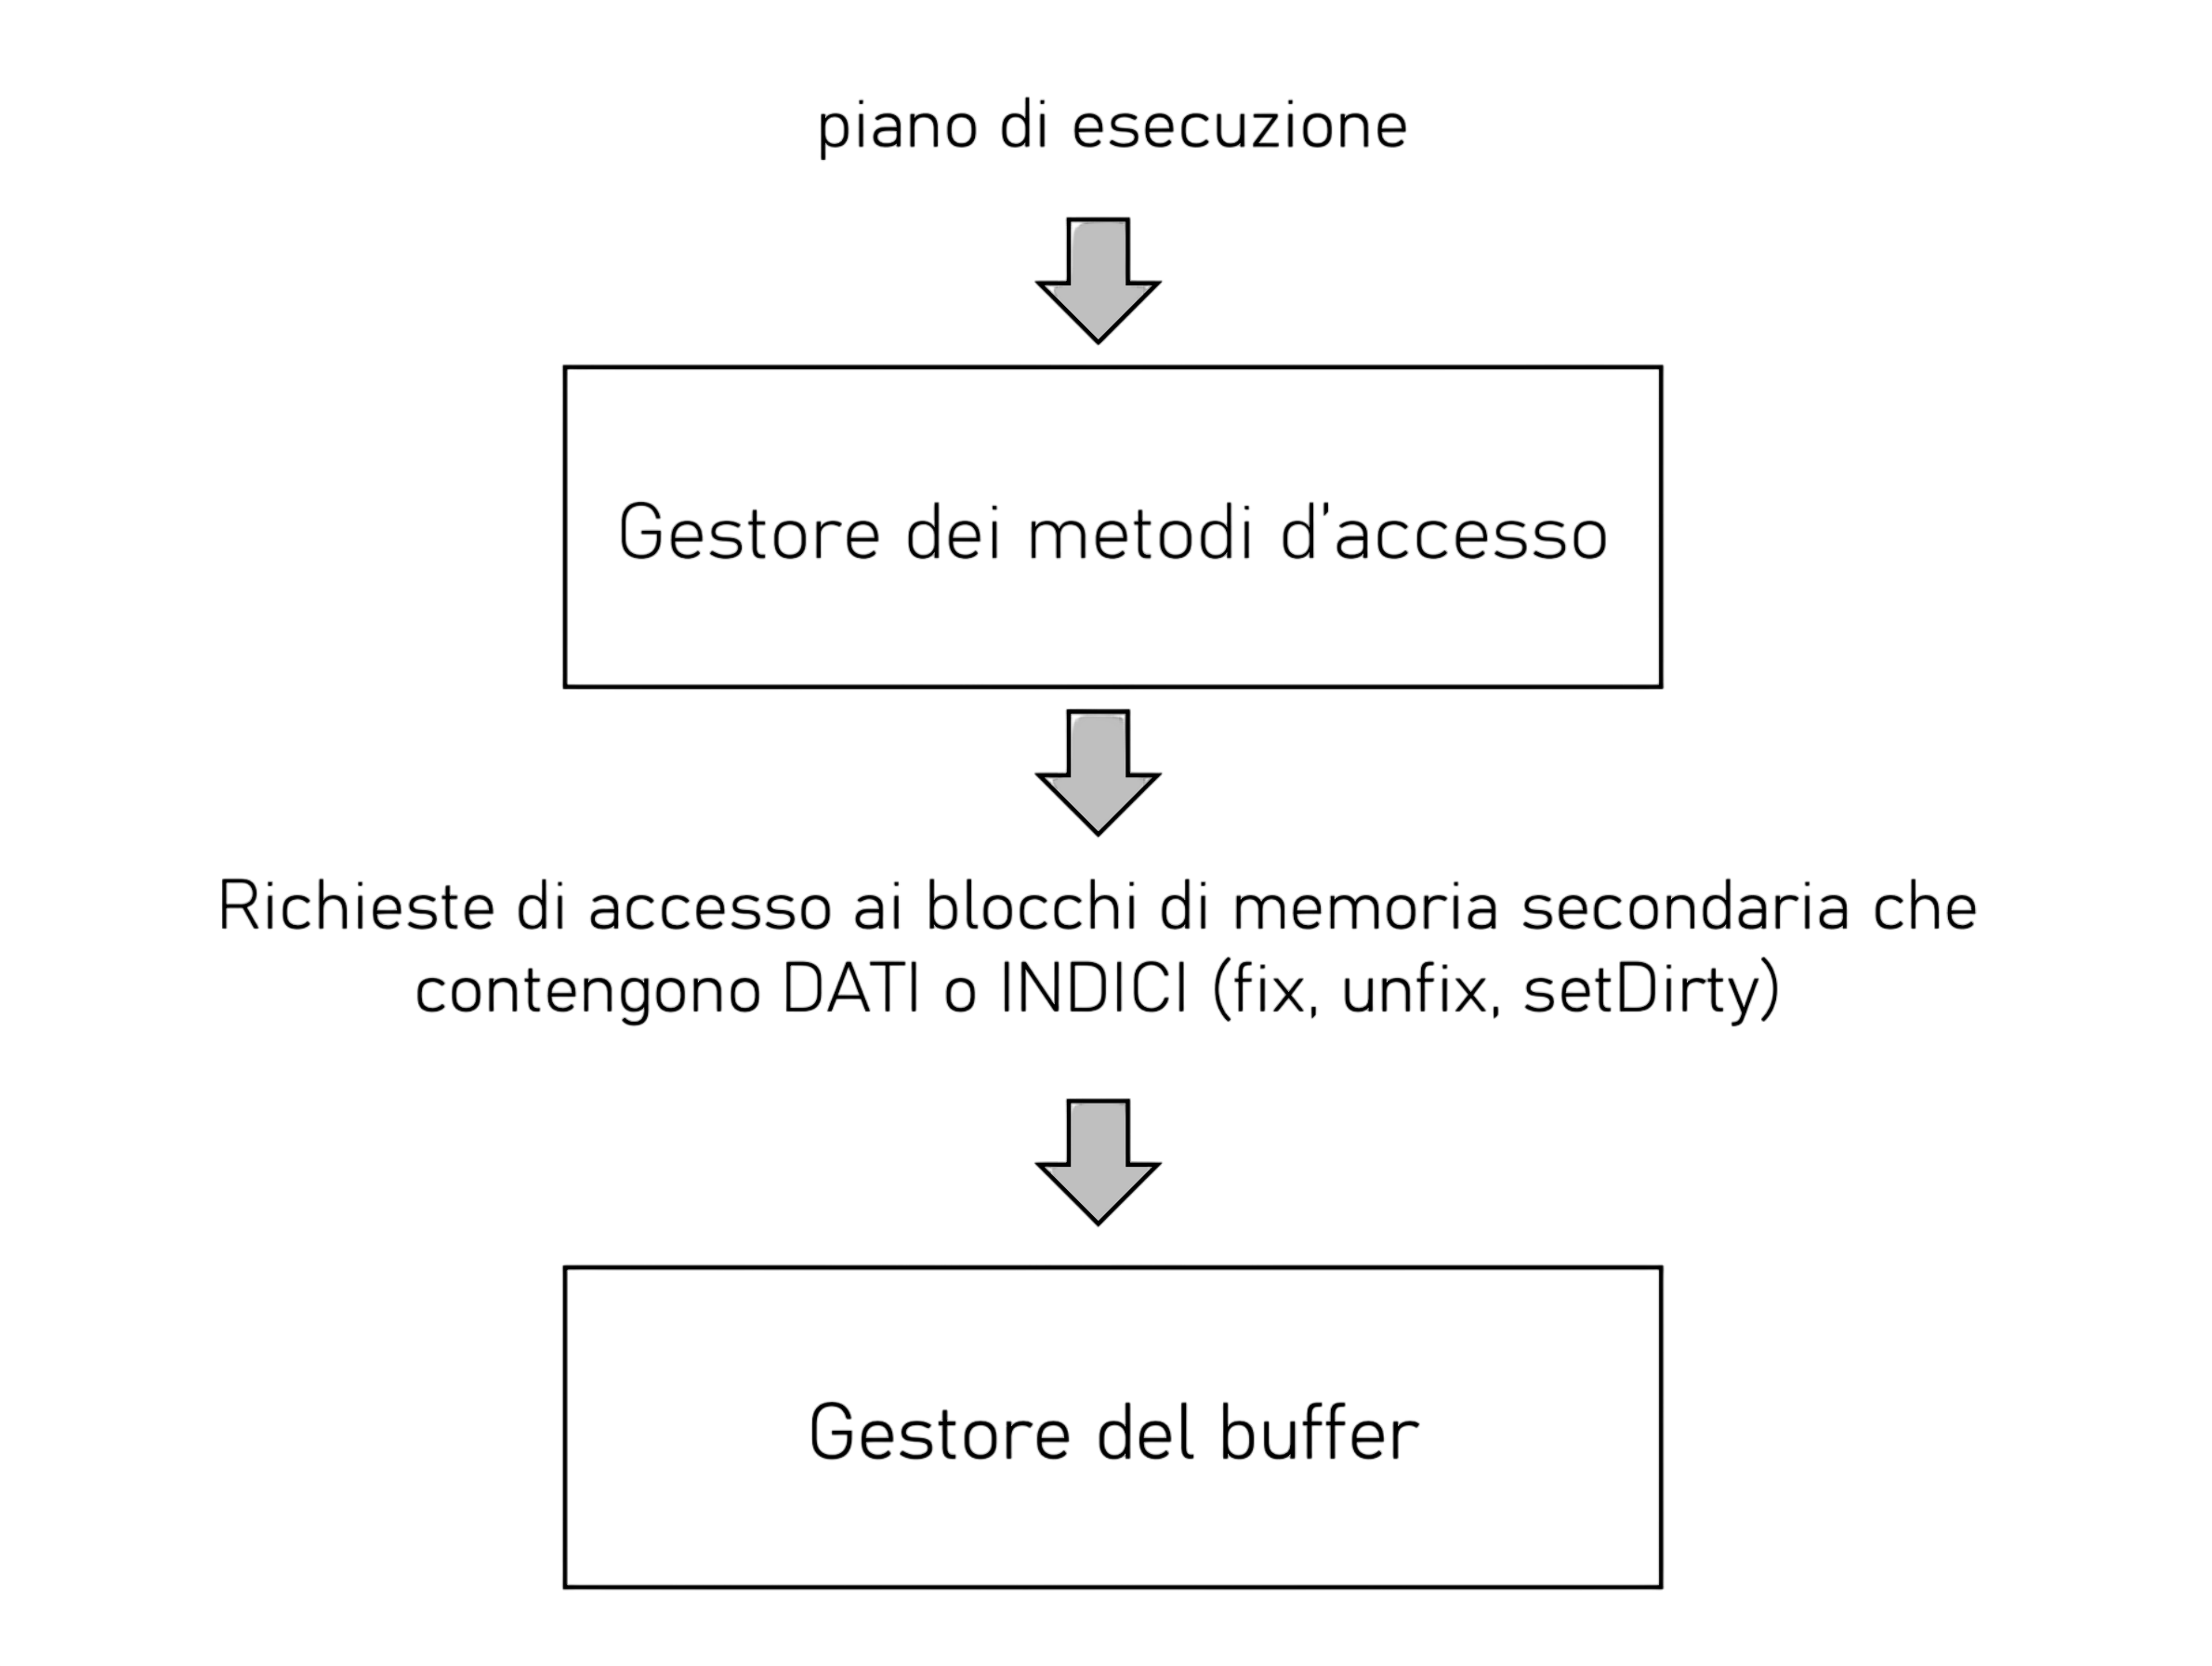
\includegraphics[width=0.6\textwidth]{images/gestore-accesso.png}
  \caption{gestore dei meotodi di accesso}
\end{figure}

\subsection{Metodi di accesso}
I metodi di accesso sono \textbf{moduli software} (es. scansione sequenziale, accesso via indice, ordinamento, varie implementazioni del join) che implementano gli algoritmi di accesso e manipolazione dei dati organizzati in specifiche strutture fisiche.

Ogni metodo di accesso conosce:
\begin{itemize}[label=$\diamond$, itemsep=\smallskipamount]
  \item \textbf{organizzazione in tuple} (o dei record di indice) nei blocchi dati (indice) salvati in memoria secondaria
  \item \textbf{organizzazione fisica interna delle pagine} sia quando contengono dati, sia quando contengono strutture fisiche di accesso (indici)
\end{itemize}

\subsection{Organizzazione di una pagina}
All'interno di una pagina sono presenti:
\begin{itemize}[label=$\triangleright$, itemsep=\smallskipamount]
  \item \textbf{informazioni utili}: dati veri e propri (tuple della tabella)
  \item \textbf{informazioni di controllo}: consentono di accedere alle informazioni utili (dizionario, bit di parità, altre informazioni del file system o della specifica struttura fisica)
\end{itemize}

\begin{figure}[H]
  \centering
  \includegraphics[width=0.6\textwidth]{images/organizzazione-pagina.png}
  \caption{organizzazione di una pagina}
\end{figure}

\begin{itemize}[label=$\Rightarrow$, itemsep=\smallskipamount]
  \item \textcolor{red}{\textbf{blocco header/trailer}}: contengono informazioni di controllo utilizzate dal file system
  \item \textcolor{violet}{\textbf{pagina header/trailer}}: contengono le informazioni di controllo relative alla specifica struttura fisica
  \item \textcolor{orange}{\textbf{dizionario di pagina}}: contiene i puntatori a ciascun dato utile elementare contenuto nella pagina
  \item \textcolor{green}{\textbf{bit di parità}}: verifica che l'informazione contenuta nella pagina sia valida
  \item \textcolor{blue}{\textbf{parte utile}}: contiene i dati
\end{itemize}

\vario{Nota}{
  Dizionari di pagina e parte utile crescono come stack contrapposti lasciando libera la parte centrale in uno spazio contiguo.
}

In caso di \textbf{tuple di lunghezza fissa}, il dizionario non è necessario: si memorizza la dimensione delle tuple e l'offset del punto iniziale.

\smallskip
In caso di \textbf{tuple di lunghezza variabile}, il dizionario memorizza l'offset di ogni tupla presente nel blocco e di ogni attributo di ogni tupla.

Molti gestori delle pagine non consentono la separazione di una tupla su più pagine:
\begin{equation*}
  \text{dimensione massima tupla} = \text{dimensione massima area disponibile su un blocco}
\end{equation*}

Alcuni gestori delle pagine consentono di distribuire una tupla su più pagine, altrimenti va gestito il caso di tuple memorizzate su più pagine.

\subsection{Operazioni sulle pagine}
Le principali operazioni che si possono eseguire sulle pagine sono:
\begin{itemize}[label=$\triangleright$, itemsep=\smallskipamount]
  \item \textbf{inserimento/aggiornamento di una tupla}:
  \begin{itemize}[label=$\diamond$, itemsep=\smallskipamount]
    \item esiste spazio contiguo sufficiente: \texttt{inserimento}
    \item non esiste spazio contiguo sufficiente, ma spazio sufficiente: \texttt{riorganizzazione dello spazio + inserimento}
    \item non esiste spazio sufficiente: \texttt{interazione con il file system per allocare nuovi blocchi per il file}
  \end{itemize}
  \item \textbf{cancellazione contenuto della pagina}
  \item \textbf{accesso a una tupla}: avviene tramite il valore della chiave o l'offset nel dizionario
  \item \textbf{accesso a un attributo di una tupla}: identificato in base all’offset e alla lunghezza del campo dopo aver identificato la tupla tramite la chiave o il suo offset 
\end{itemize}


\subsection{Strutture primarie per l'organizzazione dei file}
La struttura prmaria di un file stabilisce il criterio di disposizione delle tuple all'interno del file presente in memoria di massa:
\begin{itemize}[label=$\triangleright$, itemsep=\smallskipamount]
  \item \textbf{sequenziale}: colloca le tuple in maniera consecutiva sulla base di un criterio specifico (es. ordine di inserimento)
  \item \textbf{ad accesso calcolato}: colloca le tuple in posizioni determinate sulla base dell'esecuzione di un algoritmo di hash
  \item \textbf{ad albero}: utilizzate come strutture secondarie (indici)
\end{itemize}

\begin{figure}[H]
  \centering
  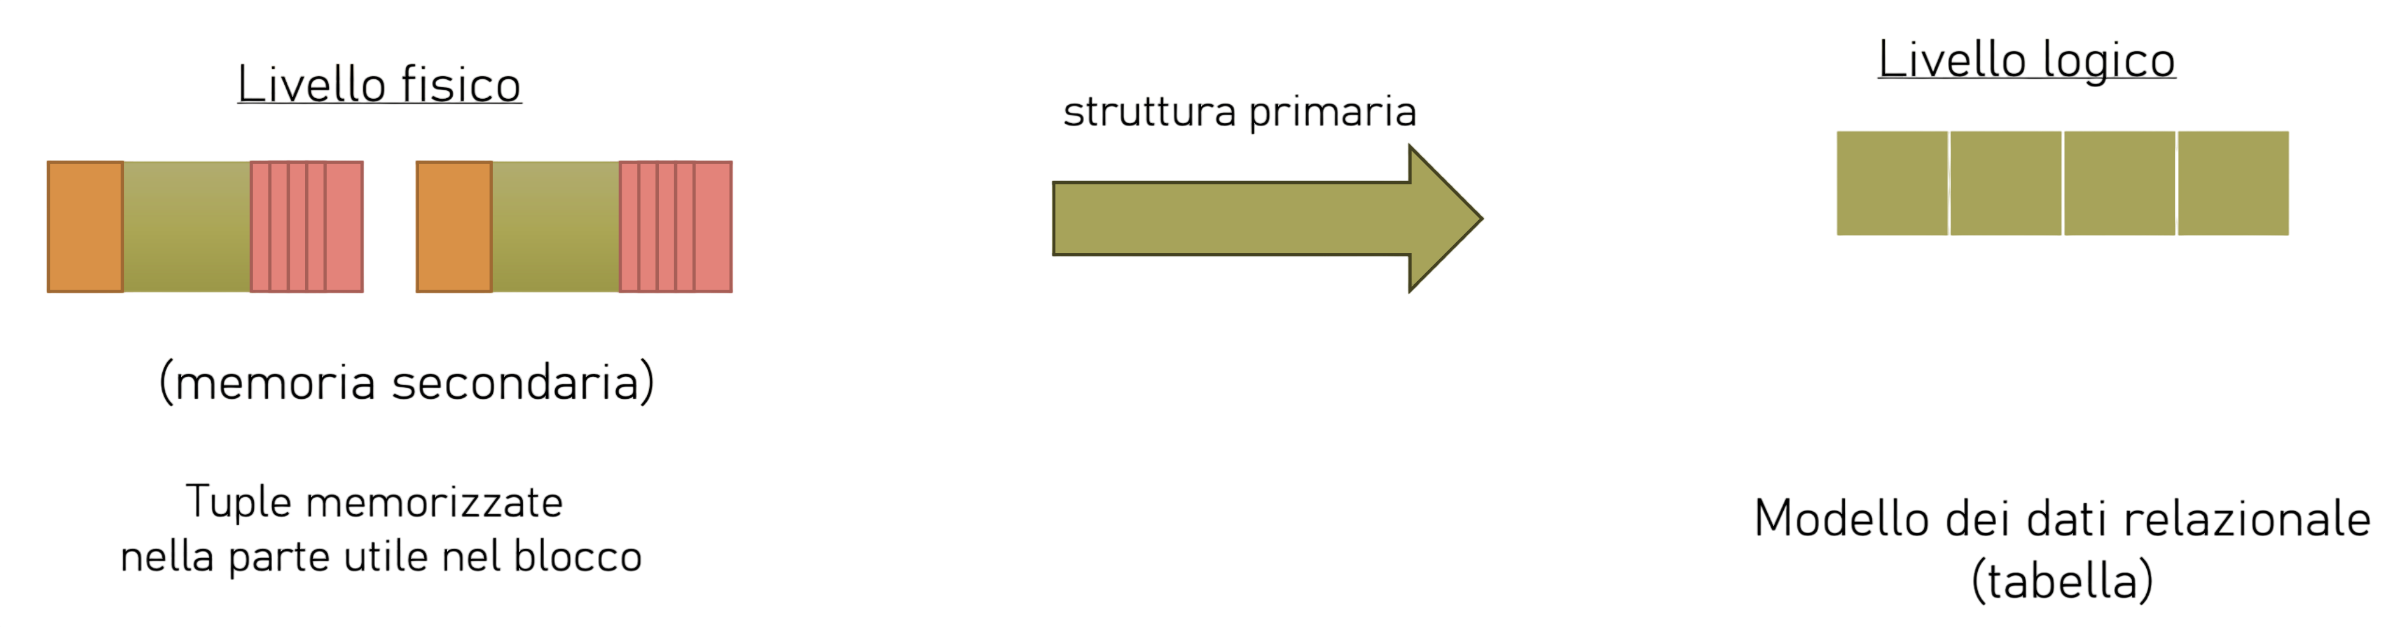
\includegraphics[width=0.7\textwidth]{images/strutture-primarie.png}
  \caption{strutture primarie per l'organizzazione dei file}
\end{figure}

\subsubsection{Struttura sequenziale}
Un file è costituito da blocchi "logicamente" consecutivi e le tuple vengono inserite nei blocchi rispettando una sequenza.

\paragraph{Struttura sequenziale disordinata}
Le tuple sono disposte in base al loro ordine di inserimento, senza alcun criterio specifico.\\[0.2ex]
Questa è la struttura più semplice e più diffusa.

\begin{itemize}[label=$\Rightarrow$, itemsep=\smallskipamount]
  \item \textbf{inserimento}:
  \begin{itemize}[label=$\diamond$, itemsep=\smallskipamount]
    \item operazione molto efficiente
    \item sufficiente mantenere un riferimento all'ultimo blocco
    \item richiede solo un accesso in memoria secondaria
    \item maggiore costo in caso di verifica dei vincoli di integrità
  \end{itemize}
  \item \textbf{ricerca}
  \begin{itemize}[label=$\diamond$, itemsep=\smallskipamount]
    \item operazione non efficiente
    \item richiede ogni volta una scansione sequenziale che consideri tutti i record, con un costo lineare nel numero di blocchi
    \item ricerca può essere fatta usando strutture secondarie (indici)
  \end{itemize}
  \item \textbf{eliminazione}
  \begin{itemize}[label=$\diamond$, itemsep=\smallskipamount]
    \item  facile una volta individuate le tuple coinvolte
    \item si marcano le tuple come "cancellate" senza riorganizzazione locale
  \end{itemize}
  \item \textbf{modifica}
  \begin{itemize}[label=$\diamond$, itemsep=\smallskipamount]
    \item  facile una volta individuate le tuple coinvolte
    \item si procede in loco se possibile, cioè quando non c’è stata nessuna modifica alla dimensione della tupla
    \item si procede con una cancellazione e un inserimento in fondo al file
  \end{itemize}
\end{itemize}

Eliminazioni e modifiche possono portare a un uso non ottimale dello spazio, siccome, si devono effettuare riorganizzazioni periodiche.

\paragraph{Struttura sequenziale ad array}
Le tuple sono disposte come in un array e la loro posizione dipende dal valore assunto in ciascuna tupla da un campo detto \textbf{indice}.\\[0.2ex]
Questa struttura è utilizzabile soltanto quando le tuple di una tabella
hanno una dimensione fissa, infatti non è quasi masi usata nei DBMS reali perchè difficilmente sono soddisfatte le condizioni per la sua applicazione.

Ad ogni file viene assegnato un numero $\mathbf{n}$ di blocchi contigui e ciascun blocco è dotato di un numero $\mathrm{m}$ di posizioni disponibili per le tuple (array bidimensionale $\mathrm{n \times m}$).\\[0.2ex]
Ogni tupla è dotata di un valore numerico $\mathrm{i}$ che rappresenta l'indice della tupla in i-esima posizione nell'array.

\begin{itemize}[label=$\Rightarrow$, itemsep=\smallskipamount]
  \item \textbf{inserimento}
  \begin{itemize}[itemsep=\smallskipamount]
    \item iniziale: l’indice $\mathbf{i}$ viene ottenuto incrementando un contatore
    \item successivo: in una posizione libera oppure alla fine del file
  \end{itemize}
  \item \textbf{cancellazione}: creano delle posizioni libere
\end{itemize}

\paragraph{Struttura sequenziale ordinata}
È un file sequenziale dove le tuple sono ordinate secondo una chiave di ordinamento (diversa dalla chiave primaria).\\[0.2ex]
Questa struttura rende efficienti le operazioni che hanno bisogno
dell'ordinamento utilizzato, ad esempio:
\begin{itemize}[label=$\circ$, itemsep=\smallskipamount]
  \item elenco ordinato
  \item range query
  \item operazioni aggregate
\end{itemize}

In caso di aggiornamento è necessario mantenere l'ordinamento, quindi servono periodiche riorganizzazioni.

\begin{itemize}[label=$\Rightarrow$, itemsep=\smallskipamount]
  \item \textbf{inserimento}
  \begin{enumerate}[itemsep=\smallskipamount]
    \item individuare il blocco B che contiene la tupla che precede, nell’ordine della chiave, la tupla da inserire
    \item se B contiene spazio sufficiente per la nuova tupla allora si inserisce la tupla in B
    \item altrimenti si aggiunge un nuovo blocco (overflow page) alla struttura e si inserisce la tupla nel nuovo blocco e si aggiusta la catena di puntatori
  \end{enumerate}
  \item \textbf{scansione sequenziale ordinata secondo la chiave}:  è sufficiente seguire i puntatori
  \item \textbf{cancellazione di una tupla}
  \begin{enumerate}[itemsep=\smallskipamount]
    \item individuare il blocco B che contiene la tupla da cancellare
    \item cancellare la tupla da B
    \item aggiustare la catena di puntatori
  \end{enumerate}
  \item \textbf{riorganizzazione}: si assegnano le tuple ai blocchi in base a opportuni coefficienti di riempimento, riaggiustando i puntatori
\end{itemize}

\esempio{struttura sequenziale}{
  Il seguente esempio mostra una struttura sequenziale ordinata secondo la chiave $\texttt{Filiale}$.
  
  \begin{figure}[H]
    \centering
    \includegraphics[width=0.7\textwidth]{images/esempio-struttura-sequenziale.png}
  \end{figure}
}

\paragraph{Indice}
Per aumentare le prestazioni degli accessi alle tuple memorizzate nelle strutture fisiche (file sequenziale), si introducono strutture ausiliarie dette strutture di accesso
ai dati (indici).\\[0.2ex]
Queste strutture velocizzano l'accesso casuale via chiave di ricerca, cioè un insieme di attributi utilizzati nell'indice della ricerca.

Ci sono due tipi di indici su file sequenziali:
\begin{itemize}[label=$\triangleright$, itemsep=\medskipamount]
  \item \textbf{indice primario}: la chiave di ordinamento del file sequenziale coincide con la chiave di ricerca dell’indice.
  
  Ogni record dell’indice primario contiene una coppia $\mathbf{\langle v_i, p_i\rangle}$, dove:
  \begin{itemize}
    \item $\mathrm{v_i}$: valore della chiave di ricerca
    \item $\mathrm{p_i}$: puntatore al primo record nel file sequenziale con chiave $\mathrm{v_i}$
  \end{itemize}

  \smallskip
  Esistono due varianti dell'indice primario:
  \begin{itemize}[itemsep=\smallskipamount]
    \item \textbf{indice denso}: per ogni occorrenza della chiave presente nel file esiste un corrispondente record nell'indice
    \item \textbf{indice sparso}: solo per alcune occorrenze della chiave presenti nel file esiste un corrispondente record nell’indice, tipicamente una per blocco
  \end{itemize}

  \smallskip
  Le operazioni che si possono eseguire su un indice primario sono:
  \begin{itemize}[label=$\diamond$, itemsep=\medskipamount]
    \item \textbf{ricerca di una tupla con chiave di ricerca K}
    \begin{itemize}[label=$\circ$, itemsep=\smallskipamount]
      \item se l'indice è denso $\mathrm{K} \rightarrow$ è presente nell'indice
      \begin{enumerate}[itemsep=\smallskipamount]
        \item scansione sequenziale dell'indice per trovare il record $\mathrm{(K, p_k)}$
        \item accesso al file attraverso il puntatore $\mathrm{p_k}$
      \end{enumerate}

      $\Rightarrow$ \hl{\textbf{costo}: 1 accesso indice + 1 accesso blocco dati}

      \esempio{ricerca con indice primario denso}{
        Un esempio di ricerca con indice primario denso è il seguente:
        \begin{figure}[H]
          \centering
          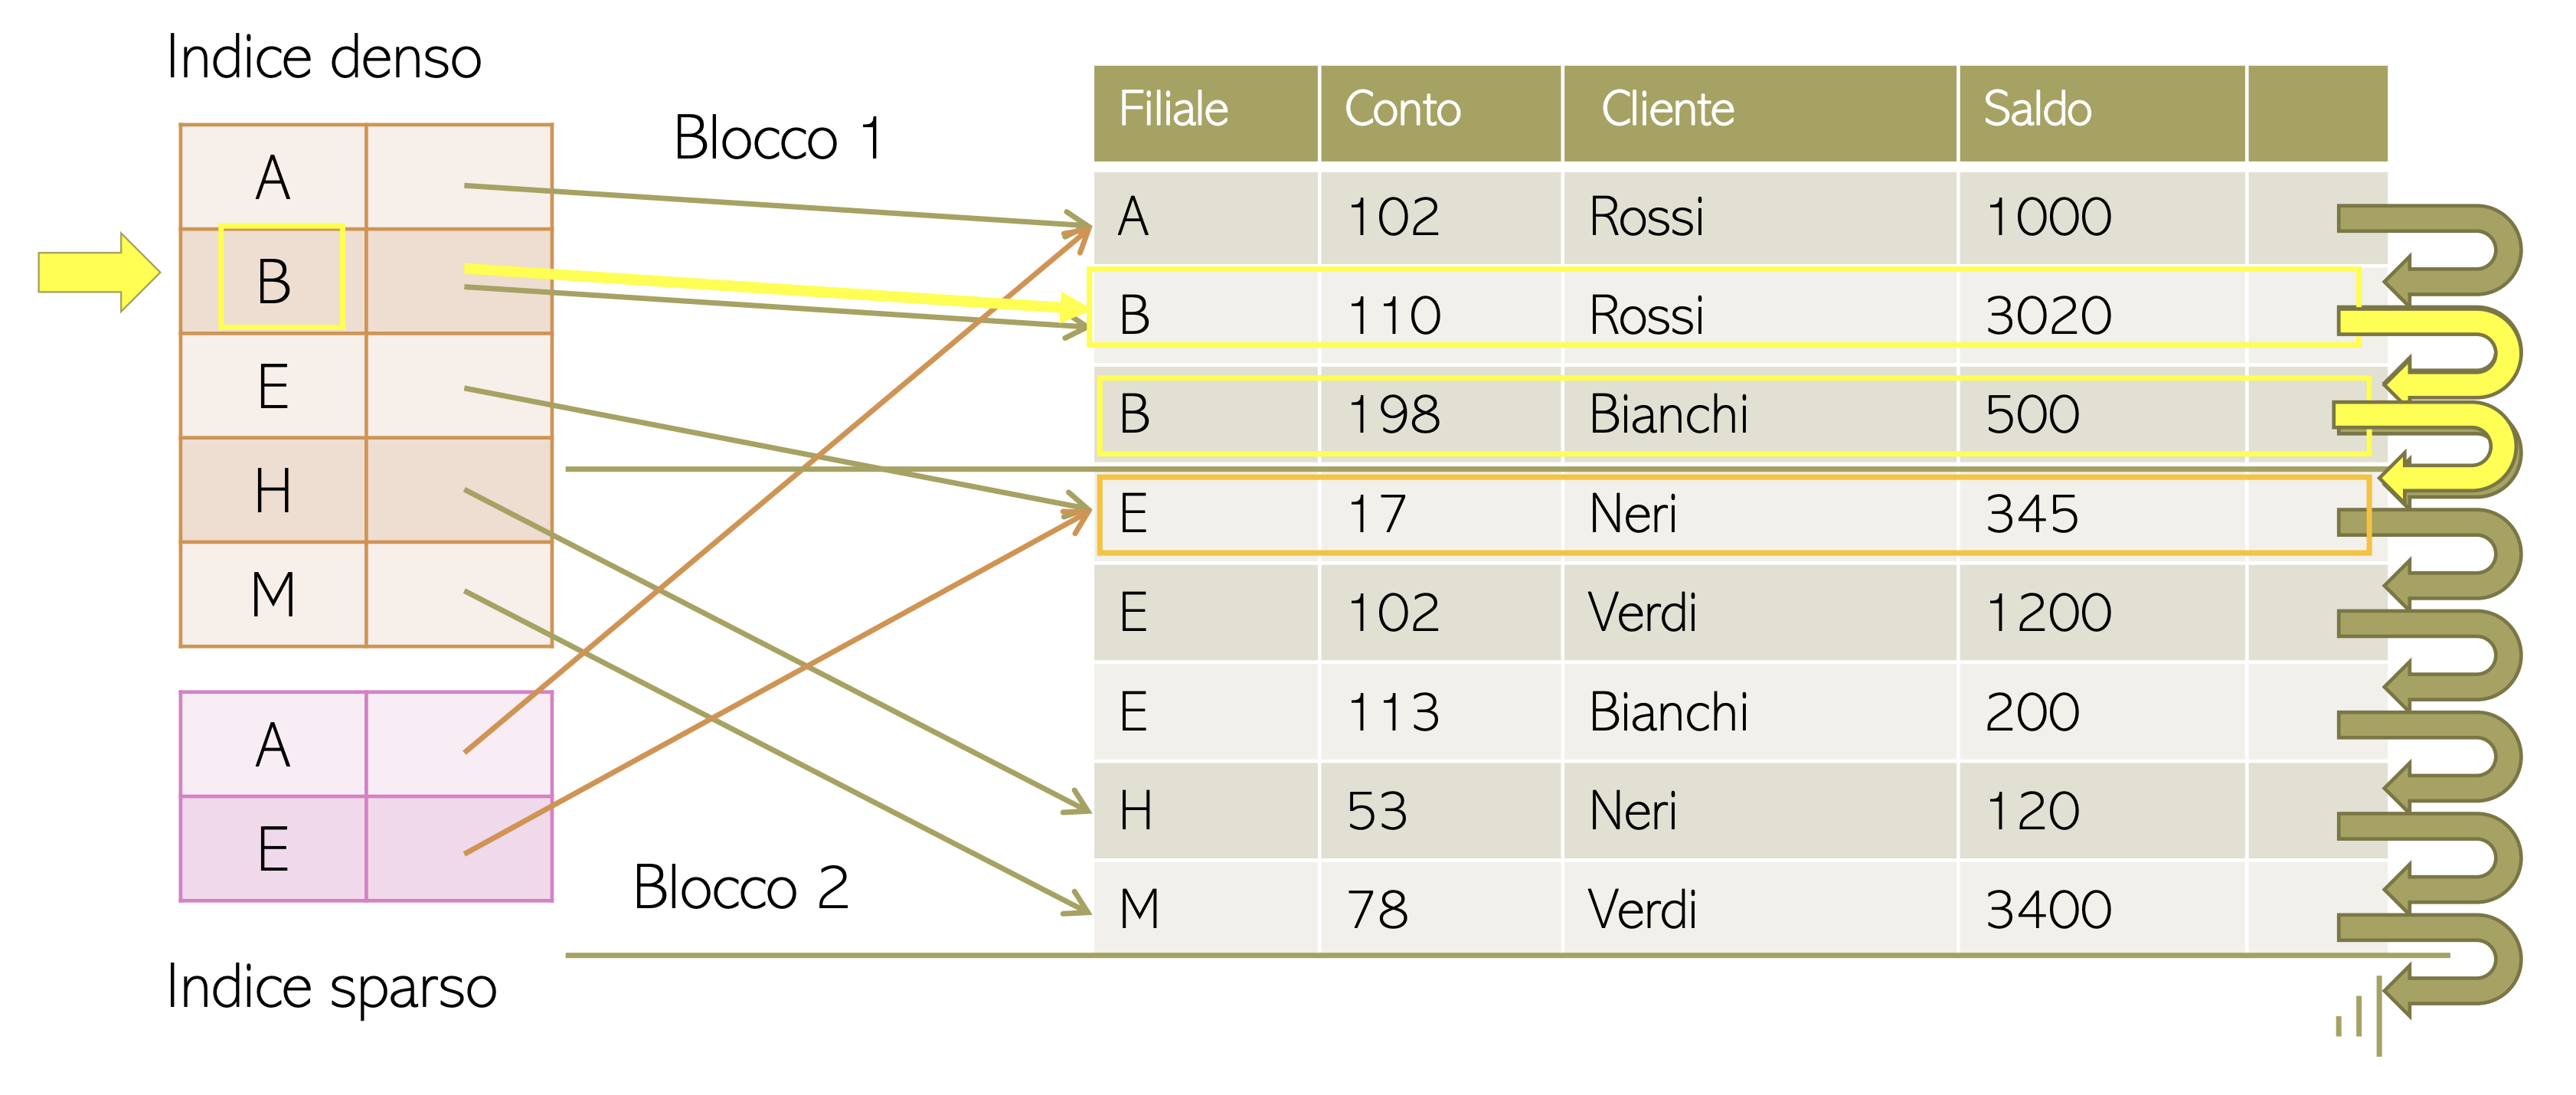
\includegraphics[width=0.6\textwidth]{images/indice-primario-denso.png}
          \caption{ricerca dei conti della filiale B}
        \end{figure}
      }

      \item se l'indice è sparso $\mathrm{K \rightarrow}$ potrebbe non essere presente nell'indice
      \begin{enumerate}[itemsep=\smallskipamount]
        \item scansione sequenziale dell'indice fino al record $\mathrm{(K', p_k)}$, dove $\mathrm{K'}$ è il valore più grande che sia minore o uguale a $\mathrm{K}$
        \item accesso al file attraverso il puntatore $\mathrm{p_k}$ e scansione del file (blocco corrente) per trovare le tuple con chiave $\mathrm{K}$
      \end{enumerate}

      $\Rightarrow$ \hl{\textbf{costo}: 1 accesso indice + 1 accesso blocco dati}

      \esempio{ricerca con indice primario sparso}{
        Un esempio di ricerca con indice primario sparso è il seguente:
        \begin{figure}[H]
          \centering
          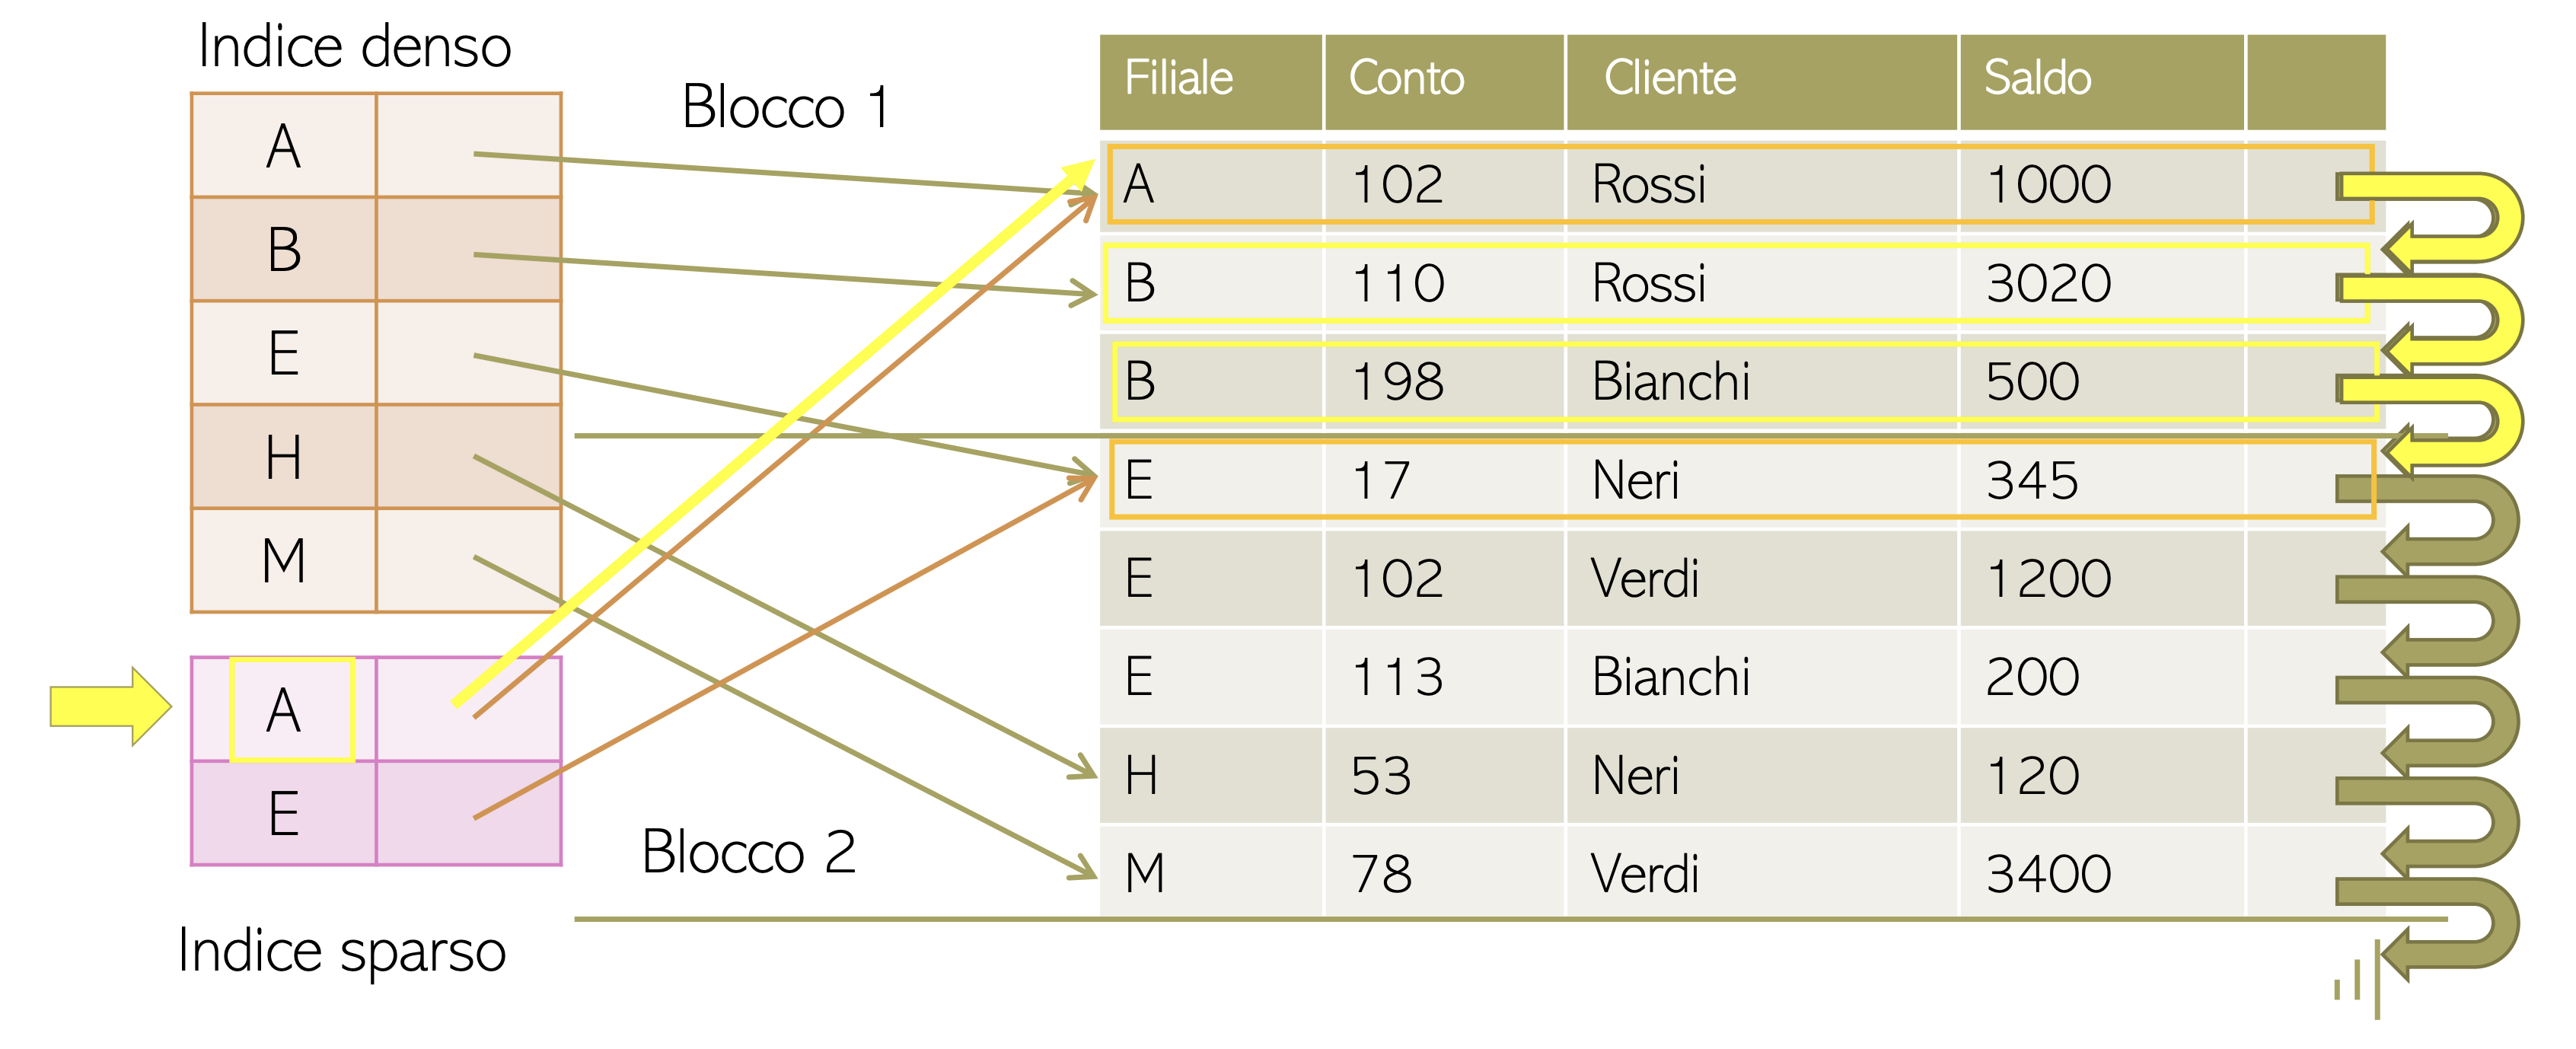
\includegraphics[width=0.6\textwidth]{images/indice-primario-sparso.png}
          \caption{ricerca dei conti della filiale B}
        \end{figure}
      }
    \end{itemize}

    \item \textbf{inserimento di un record nell'indice}
    \begin{itemize}[label=$\circ$, itemsep=\smallskipamount]
      \item \textbf{indice è denso}: inserimento nell'indice avviene solo se la tupla inserita nel file ha un valore di chiave K che non è già presente
      \item \textbf{indice è sparso}: inserimento avviene solo quando, per effetto dell'inserimento di una nuova tupla, si aggiunge un blocco dati alla struttura (negli altri casi rimane invariato)
    \end{itemize}

    \smallskip
    Gli indici sono costosi, quindi, bisogna fare un compromesso sul numero di indici da mantenere e il numero di attributi ad accesso sequenziale.

  \item  \textbf{cancellazione} di un record nell’indice
  \begin{itemize}[label=$\circ$, itemsep=\smallskipamount]
    \item \textbf{indice è denso}: cancellazione nell'indice avviene solo se la tupla cancellata nel file è l'ultima tupla con valore di chiave $\mathrm{K}$
    \item \textbf{indice è sparso}: cancellazione nell'indice avviene solo quando $\mathrm{K}$ è presente nell'indice e il corrispondente blocco viene eliminato
    
    Nel caso in cui il blocco sopravvive, va sostituito $\mathrm{K}$ nel record dell'indice con il primo valore $\mathrm{K'}$ presente nel blocco.
  \end{itemize}
\end{itemize}
\item \textbf{indice secondario}: la chiave di ordinamento e la chiave di ricerca sono diverse.

Ogni record dell'indice secondario contiene una coppia $\mathrm{\langle v_i, p_i \rangle}$, dove:
\begin{itemize}
  \item $\mathrm{v_i}$: valore della chiave di ricerca
  \item $\mathrm{p_i}$: puntatore al bucket di puntatori che individuano nel file sequenziale tutte le tuple con chiave $\mathrm{v_i}$
\end{itemize}

Gli indici secondari sono sempre densi perchè non si può sfruttare l'ordinamento delle tuple.

Le operazioni che si possono eseguire su un indice secondario sono:
\begin{itemize}[label=$\diamond$, itemsep=\medskipamount]
  \item \textbf{ricerca di una tupla con chiave di ricerca} $\mathbf{K}$
  \begin{enumerate}[itemsep=\smallskipamount]
    \item scansione sequenziale dell'indice per trovare il record $\mathrm{(K, p_k)}$
    \item accesso al bucket $\mathrm{B}$ di puntatori attraverso il puntatore $\mathrm{B}$
    \item accesso al file attraverso i puntatori del bucket $\mathrm{B}$
  \end{enumerate}
  
  $\Rightarrow$ \hl{\textbf{costo}: 1 accesso indice + 1 accesso al bucket + n accessi alle pagine dati} (n è il numero di puntatori nel bucket B)

  \esempio{ricarca con indice secondario}{
    Un esempio di ricerca con indice secondarioè il seguente:
    \begin{figure}[H]
      \centering
      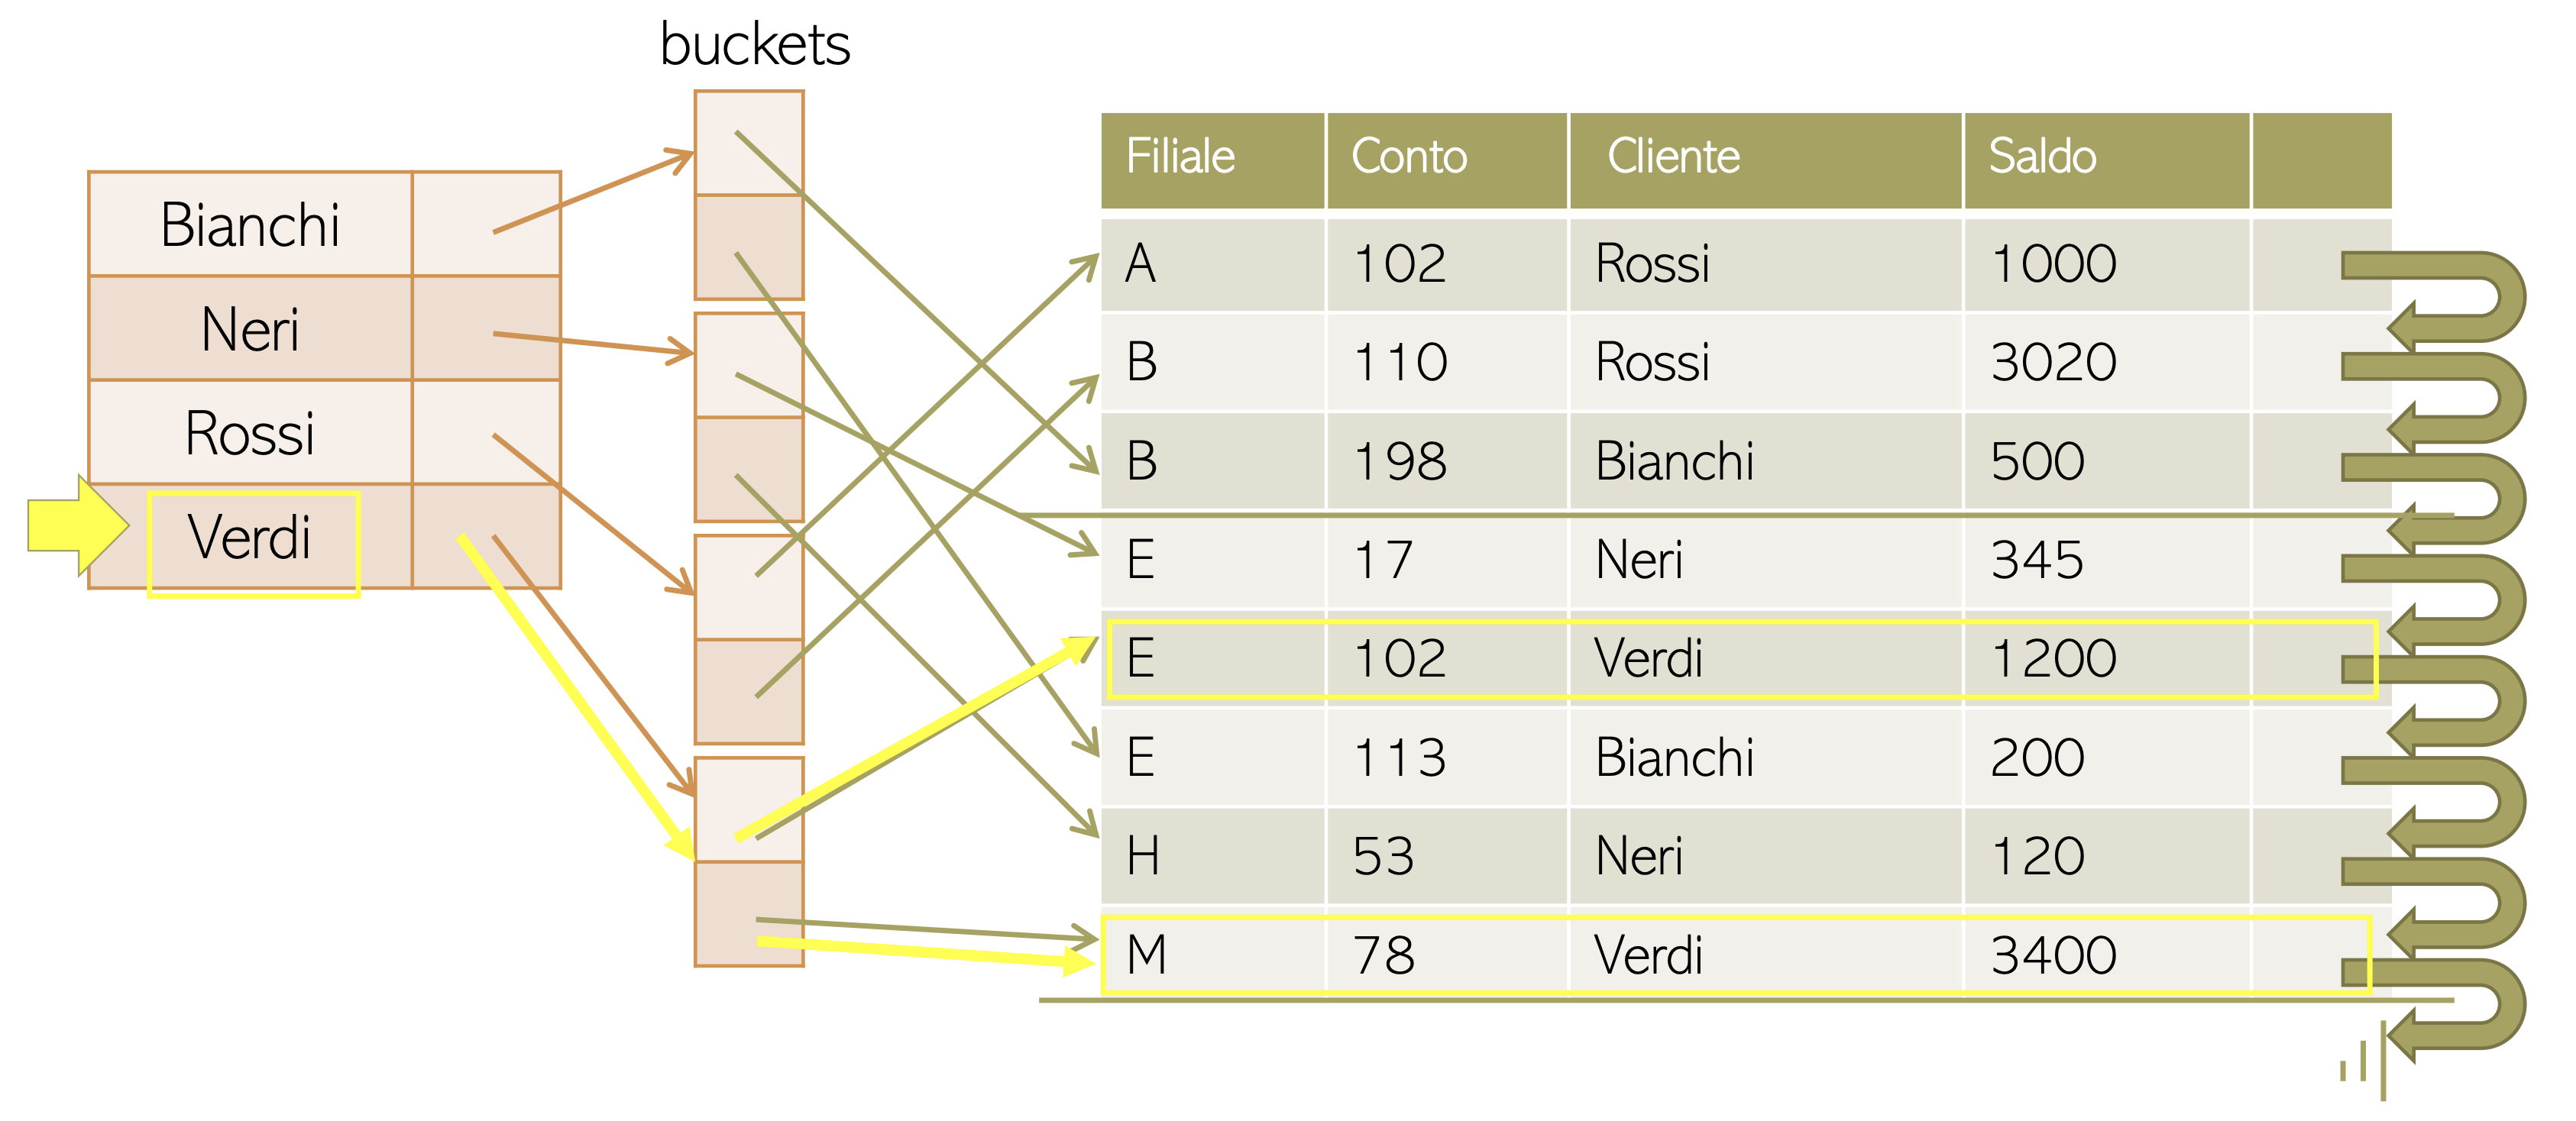
\includegraphics[width=0.6\textwidth]{images/indice-secondario.png}
      \caption{ricerca dei conti della filiale B}
    \end{figure}
  }

  \item  \textbf{inserimento} e \textbf{cancellazione}: si effettuano gli stessi passi dell'inserimento e della cancellazione in un indice primario denso, con in più l'aggiornamento dei bucket
\end{itemize}
\end{itemize}

\subsubsection{Struttura ad albero}
Quando l'indice aumenta di dimensioni non si può più gestire in memoria centrale, di conseguenza deve essere gestito in memoria secondaria.\\[0.2ex]
Per migliorare le prestazioni degli accessi a un indice di grandi dimensioni, si utilizza il $\verb|B+ tree|$, in cui:
\begin{itemize}[label=$\triangleright$, itemsep=\smallskipamount]
  \item ogni nodo viene memorizzato in una pagina della memoria secondaria
  \item legami tra nodi = puntatori a pagina
  \item sono presenti molti figli e di conseguenza ha pochi livelli
  \item albero bilanciato: la lunghezza dei percorsi che collegano la radice ai nodi foglia è costante
  \item inserimenti e cancellazioni non alterano le prestazioni dell'accesso ai dati: l'albero si mantiene bilanciato
\end{itemize}

\paragraph{Struttura}
La struttura di un $\verb|B+ tree|$ con fan-out = n (n figli per nodo) è la seguente:
\begin{itemize}[label=$\triangleright$, itemsep=\medskipamount]
  \item \textbf{nodo foglia}
  
  \begin{figure}[H]
    \centering
    \includegraphics[width=0.5\textwidth]{images/nodo-foglia-BTree.png}  
  \end{figure}

  Può contenere fino a $\mathbf{n - 1}$ valori ordinati di chiave di ricerca e fino a $\mathbf{n}$ puntatori ai dati.\\[0.2ex]
  Ogni nodo foglia ha un vincolo di ordinamento, cioè:
  \begin{itemize}[label=$\circ$, itemsep=\smallskipamount]
    \item chiavi dentro a un nodo foglia sono ordinate
    \item nodi foglia sono ordinati tra di loro.
    
    Dati due nodi foglia $\mathrm{L_i}$ e $\mathrm{L_j}$ con $\mathrm{i < j}$, allora:
    \begin{equation*}
      \mathrm{\forall k_i \in L_i; \quad \forall k_s \in L_j; \quad k_t < k_s}
    \end{equation*}
  \end{itemize}

  Il puntatore $\mathrm{p_m}$ del nodo $\mathrm{L_i}$ punta al nodo foglia $\mathrm{L_{i+1}}$ (se esiste):

  \begin{figure}[H]
    \centering
    \includegraphics[width=0.5\textwidth]{images/puntatore-nodo-foglia-BTree.png}
  \end{figure}

  Una variante del $\verb|B+ tree|$ è quella in cui i nodi foglia contengono direttamente le tuple.

  In questo caso si ha una struttura fisica integrata.


  \item \textbf{nodo intermedio}: è una sequenza di $\mathrm{m' \leq n}$ valori ordinati di chiave (può contenere fino a $\mathrm{n}$ puntatori a nodo).

  Ogni nodo chiave $\mathrm{K_i}$ è seguita da un puntatore $\mathrm{p_i}$:
  \begin{figure}[H]
    \centering
    \includegraphics[width=0.5\textwidth]{images/nodo-intermedio-BTree.png}
  \end{figure}
\end{itemize}

\paragraph{Vincoli di riempimento}
Il fan-out è un parametro che fornisce il limite massimo, ma bisogna anche fornire un limite minimo per evitare che i nodi siano troppo vuoti e sono chiamati \textbf{vincoli di riempimento}:
\begin{itemize}[label=$\diamond$, itemsep=\medskipamount]
  \item \textbf{vincoli per i nodi foglia}: ogni nodo foglia può contenere un numero di valori di chiavi ($\mathrm{\# \ chiavi}$) vincolato
  \begin{equation*}
    \mathrm{\left\lceil \frac{n - 1}{2} \right\rceil \leq \# \ chiavi \leq n - 1}
  \end{equation*}
  \item \textbf{vincoli per i nodi intermedi}: ogni nodo intermedio può contenere un numero di puntatori ($\mathrm{\# \ puntatori}$) vincolato
  \begin{equation*}
    \mathrm{\left\lceil \frac{n}{2} \right\rceil \leq \# \ puntatori \leq n}
  \end{equation*}
\end{itemize}

\esempio{utilizzo del \texttt{B+-tree}}{
  Consideriamo ad esempio un B+-Tree con fan-out = 4 con contenuto:
  \[
    \mathrm{A, B, D, E, F, G, L, M, N, P}
  \] 
  Il fan-out ci dice che per:
  \begin{itemize}
    \item \textbf{nodi foglia}: vincoli di riempimento sono
      \[
        2 \le \#chiavi \le 3
      \] 

    \item \textbf{nodi intermedi}: vincoli di riempimento sono
      \[
        2 \le \#puntatori \le 4
      \]

    \item \textbf{radice}: unico nodo per cui i vincoli di riempimento \textbf{minimi}
      non si applicano
  \end{itemize}
  \begin{figure}[H]
    \centering
    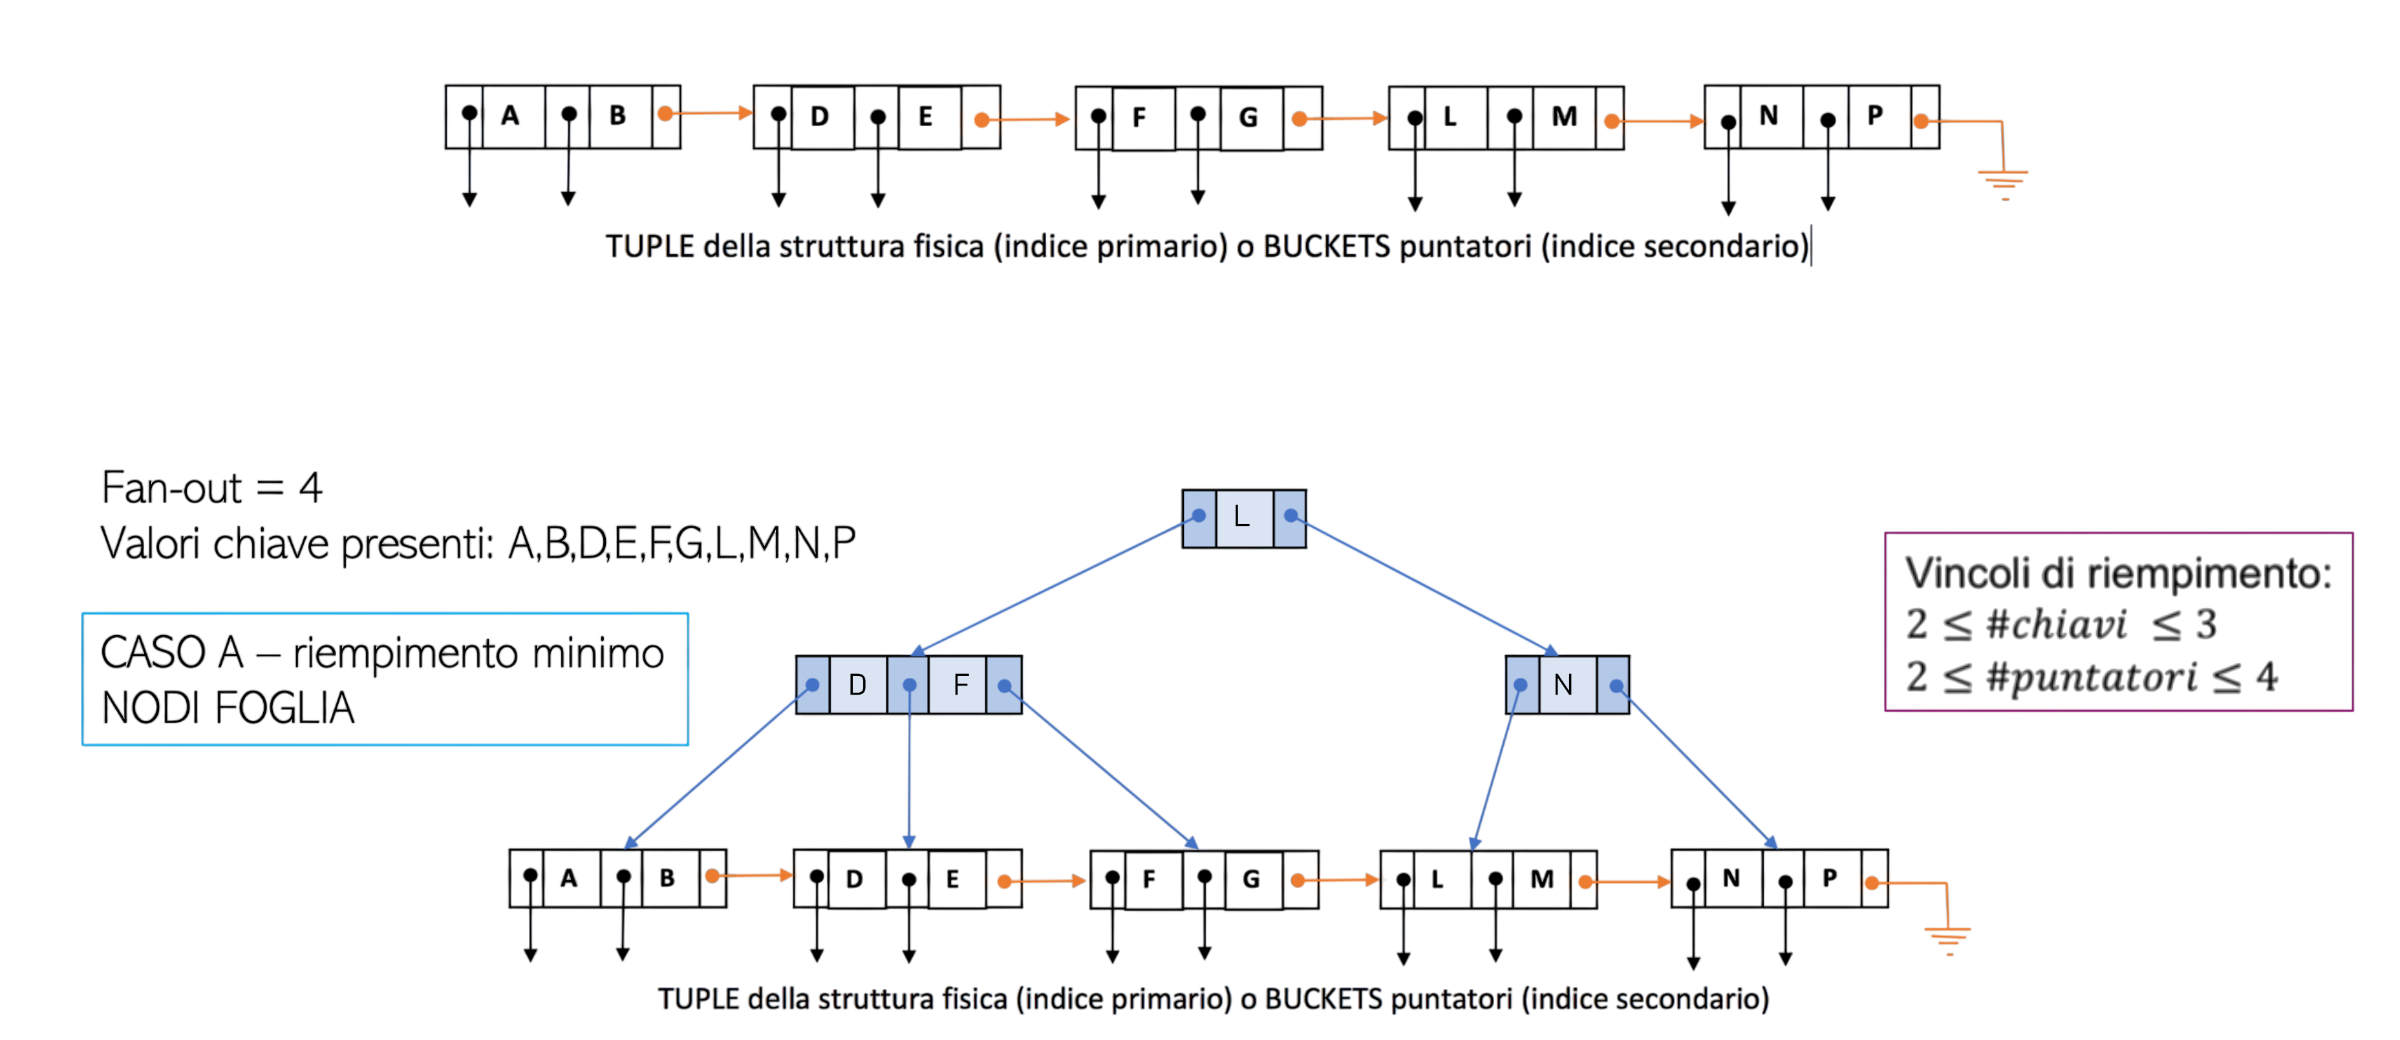
\includegraphics[width=0.8\textwidth]{images/b_plus_tree_esempio.png}
    \caption{Esempio di B+-Tree con vincolo di riempimento minimo}
  \end{figure}

  La radice \( \mathrm{L} \) punta:
  \begin{itemize}[label=$\diamond$, itemsep=\smallskipamount]
    \item a sinistra: al sottoalbero con chiave \( \mathrm{K < "L"} \) 
    \item a destra: al sottoalbero con chiave \( \mathrm{K \ge "L"} \)
  \end{itemize}

  \smallskip
  I figli puntano alle tuple con chiave uguale a quella del nodo foglia.
  
  In questo caso l'albero per chiavi desiderate rispetta il vincolo di riempimento minimo.
  
  Per rispettare il vincolo di riempimento massimo bisogna fare un altro albero:
  \begin{figure}[H]
    \centering
    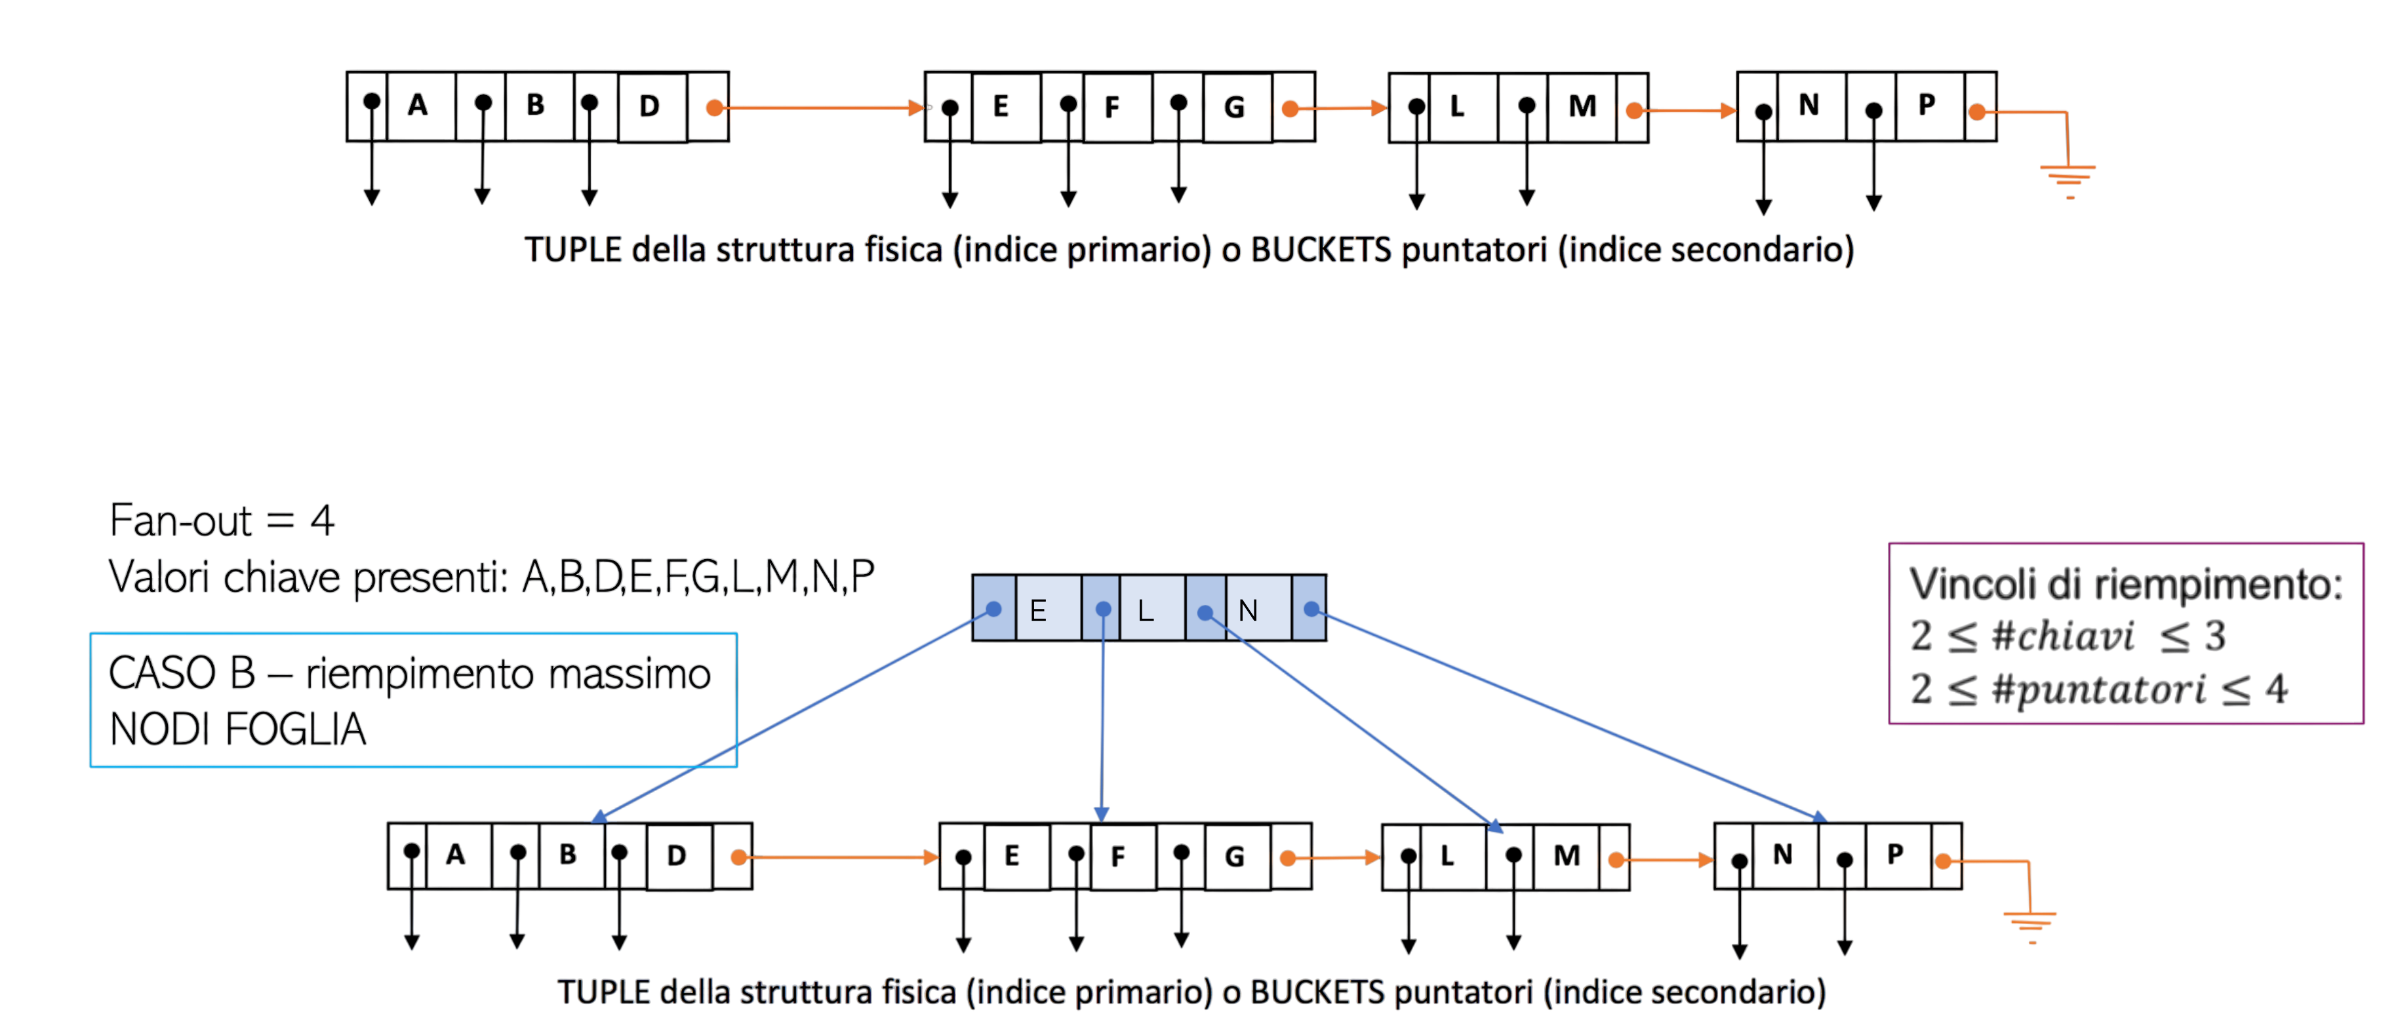
\includegraphics[width=0.8\textwidth]{images/b_plus_tree_esempio2.png}
    \caption{Esempio di B+-Tree con vincolo di riempimento massimo}
  \end{figure}

  Le etichette per la radice sono assegnate secondo:
  \begin{itemize}[label=$\circ$, itemsep=\smallskipamount]
    \item sinistra: Chiavi comprese tra: \( \mathrm{"E" \le K < "L"} \) 
    \item centro: Chiavi comprese tra \( \mathrm{"L" \le K < "N"} \)
    \item destra: Chiavi \( \mathrm{K \ge "N"} \)
  \end{itemize}
}

\paragraph{Operazione: ricerca con chiave K}
Per effettuare la ricerca di una tupla con chiave di ricerca K si effettuano i seguenti passi:
\begin{enumerate}[itemsep=\medskipamount]
  \item \textbf{cercare nel nodo radice il più piccolo valore di chiave maggiore di K}
  \begin{itemize}[label=$\triangleright$, itemsep=\medskipamount]
    \item se il valore esiste ($\mathrm{value = k_i}$) $\rightarrow$ seguire il puntatore $\mathrm{p_i}$
    \begin{figure}[H]
      \centering
      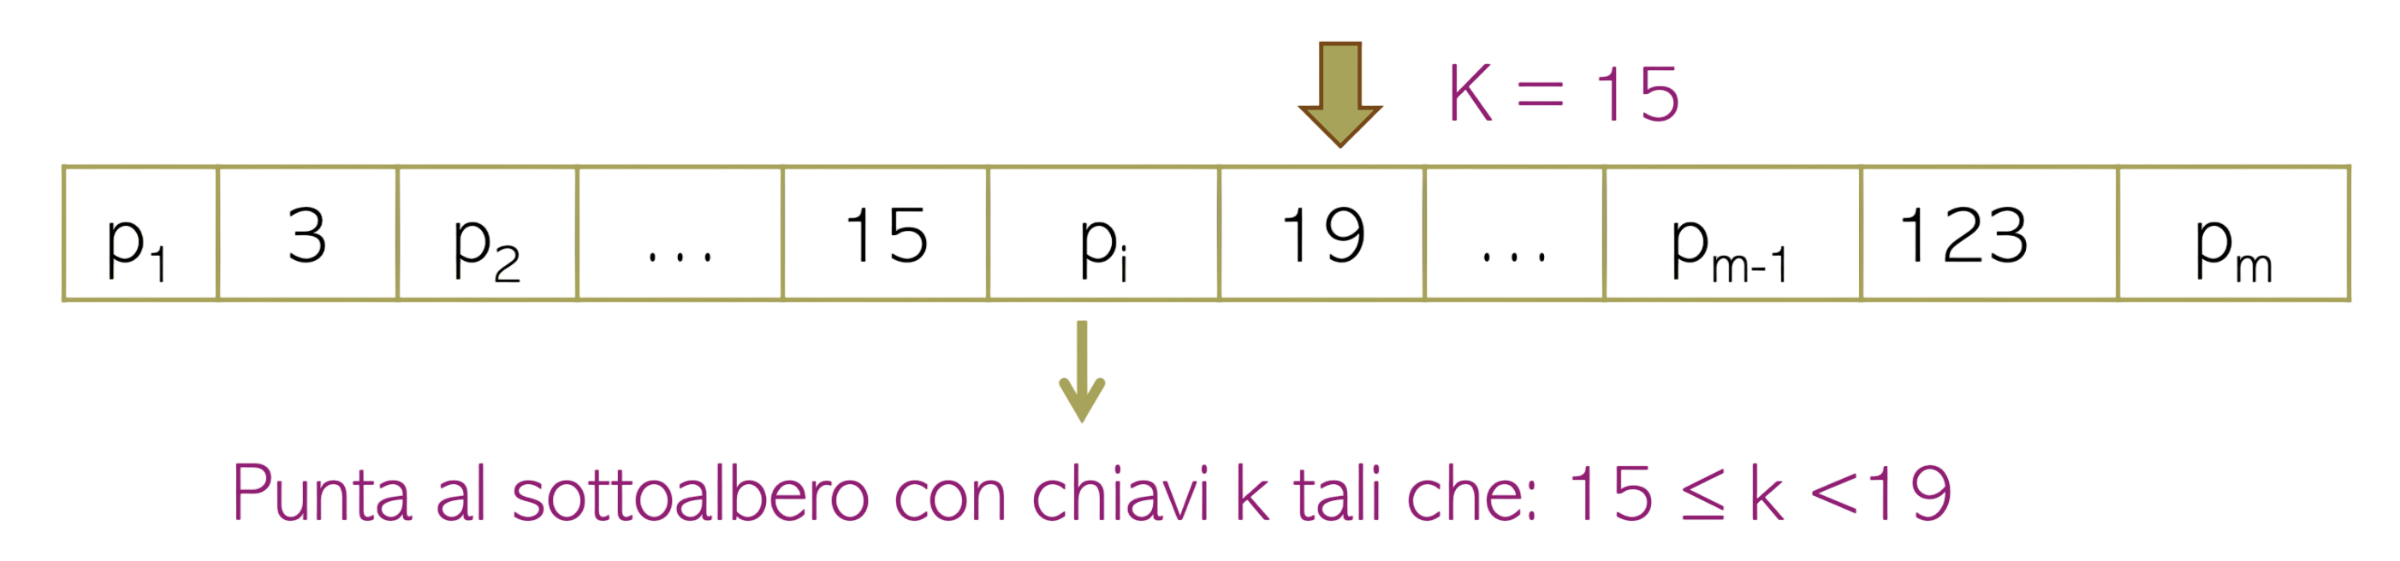
\includegraphics[width=0.5\textwidth]{images/ricerca-chiave-k-nodoRadice1.png}
    \end{figure}
    \item se il valore non esiste $\rightarrow$ seguire puntatore $\mathrm{p_m}$
    \begin{figure}[H]
      \centering
      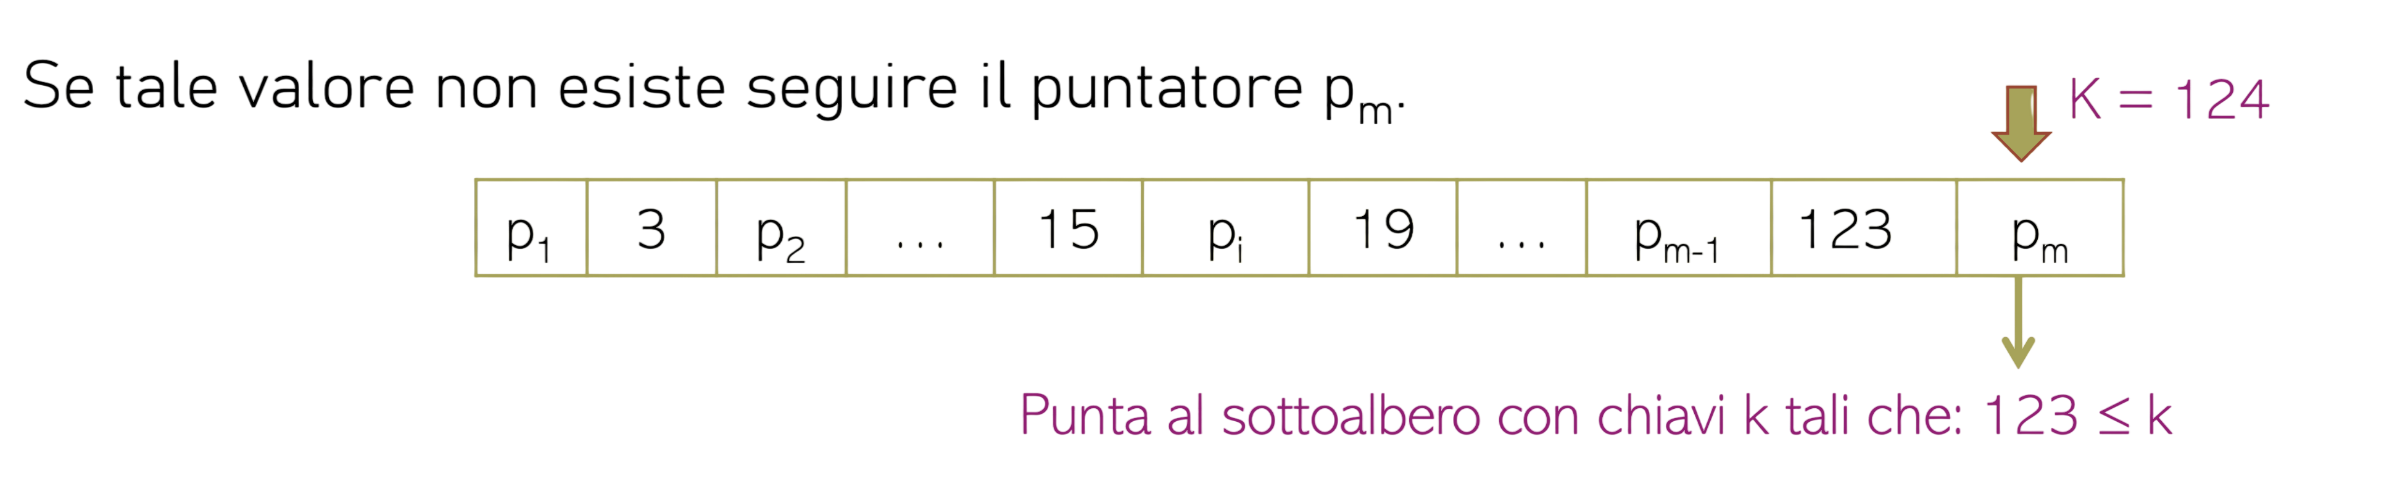
\includegraphics[width=0.5\textwidth]{images/ricerca-chiave-K-nodoRadice2.png}
    \end{figure}
  \end{itemize}
  \item \textbf{cercare il valore K (se nodo raggiunto = nodo foglia) e seguire il corrispondente puntatore verso le tuple} o \textbf{riprendere il passo 1 (se non esistono)}
  \begin{figure}[H]
    \centering
    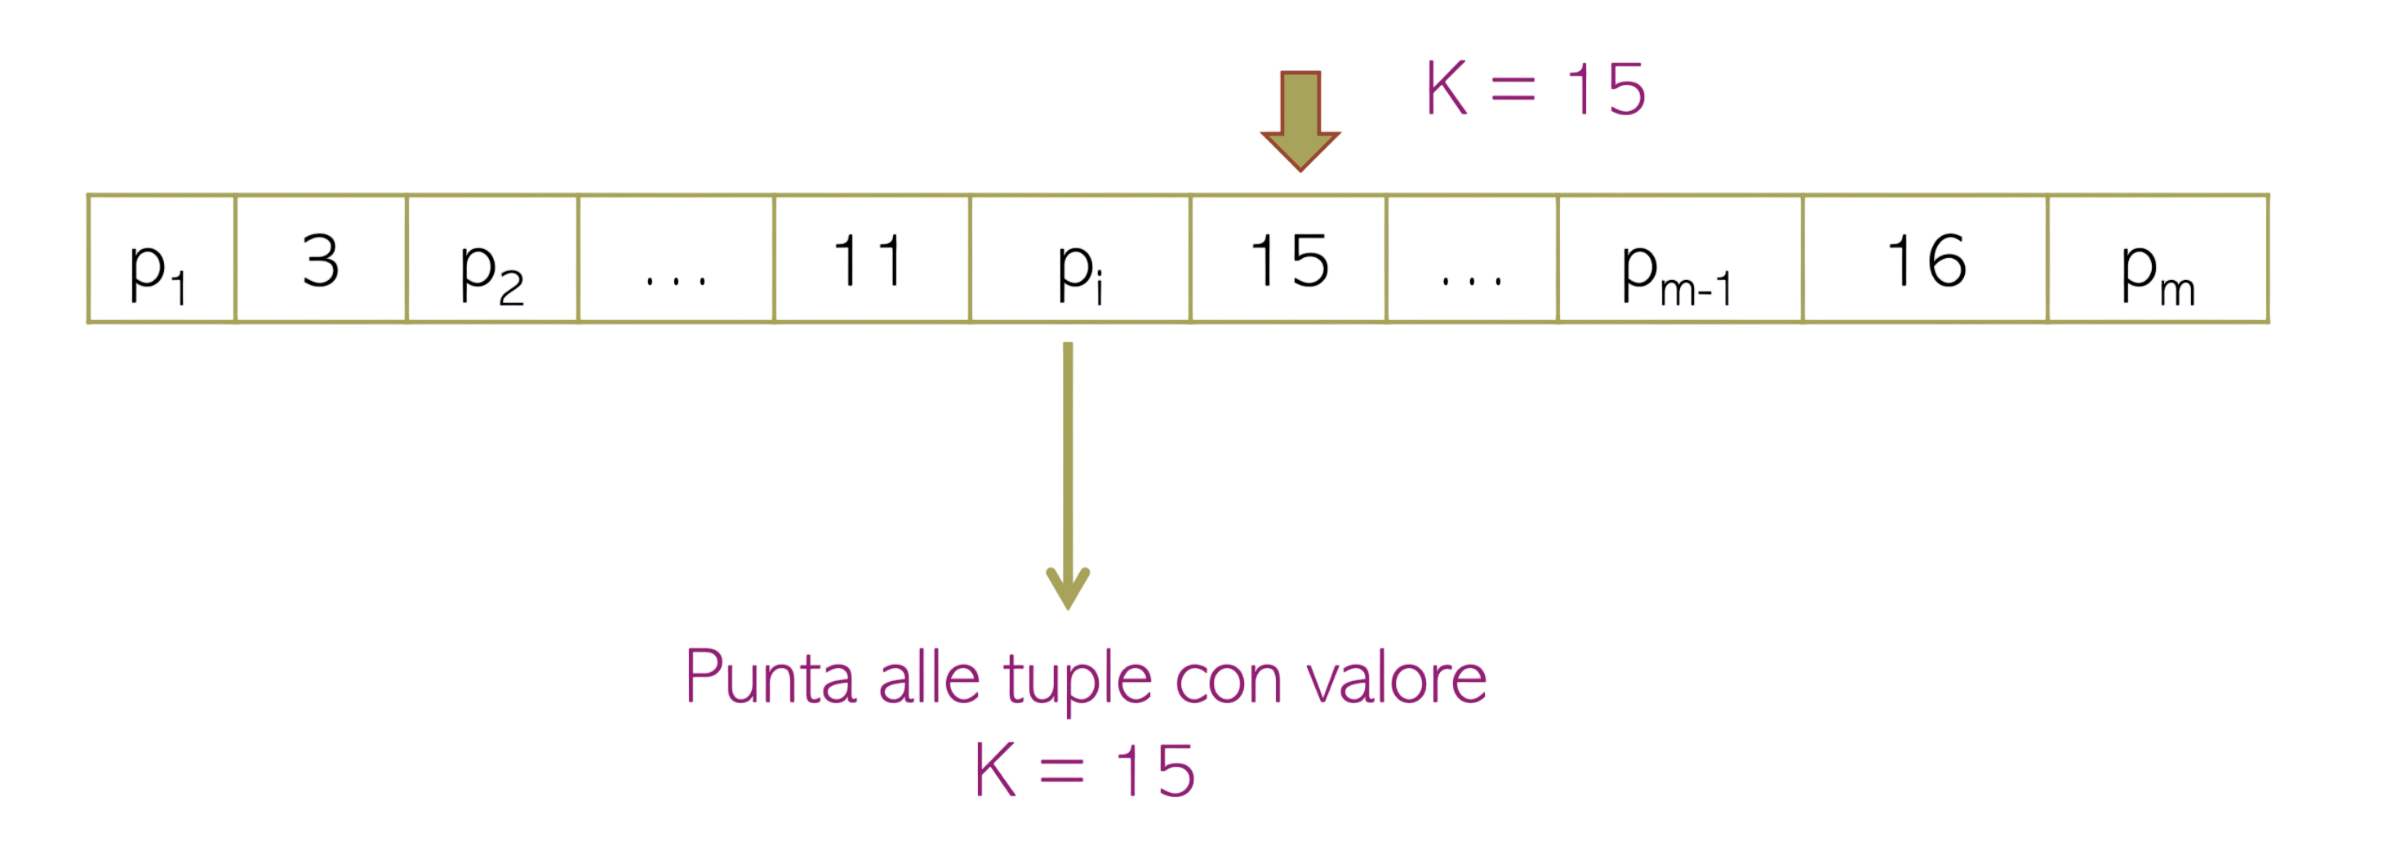
\includegraphics[width=0.5\textwidth]{images/ricerca-chiave-k-nodoFoglia.png}
  \end{figure}
\end{enumerate}

\esempio{ricerca di una tupla con chiave di ricerca K = "G"}{
  \begin{figure}[H]
    \centering
    \includegraphics[width=1.0\textwidth]{images/esempio-ricerca-chiave-k.png}
  \end{figure}
}

Il costo della ricerca dipende dalla profondità dell'albero in termini di \textbf{accessi alla memoria secondaria}, dove ogni metodo rappresenta un blocco.\\[0.2ex]
Il \underline{costo in una struttura ad albero} è pari alla profondità dell'albero, che nel $\verb|B+ tree|$ è indipendente dal percorso ed è funzione del fan-out $\mathrm{n}$ e del numero di valori di chiave presente nell'albero $\mathrm{\# \ valoriChiave}$.
\begin{equation*}
  \mathrm{prof_{B+ tree}} \leq \underbrace{1}_{\text{radice}} + \underbrace{\log_{\left\lceil \frac{n}{2} \right\rceil} \left( \frac{\overbrace{\# \text{valoriChiave}}^{\text{nodi foglia massimi}}}{\left\lceil \frac{n - 1}{2} \right\rceil} \right)}_{\text{\# livelli}}
\end{equation*}

\paragraph{Operazione: inserimento}
Per inserire una tupla in un $\verb|B+ tree|$ bisogna mantenere i vincoli di riempimento, quindi, vengono eseguiti i seguenti passi:
\begin{enumerate}[itemsep=\medskipamount]
  \item \textbf{ricerca del nodo foglia NF dove K va inserito}
  \item 
  \begin{itemize}[label=$\triangleright$, itemsep=\medskipamount]
    \item se K è presente in NF:
    \begin{itemize}[label=$\diamond$, itemsep=\smallskipamount]
      \item se è \textbf{indice primario} $\rightarrow$ non si fa nessuna azione
      \item se è \textbf{indice secondario} $\rightarrow$ si aggiornano i bucket dei puntatori
    \end{itemize}
    \item se k non è prensente in NF:
    \begin{itemize}[label=$\diamond$, itemsep=\smallskipamount]
      \item se è \textbf{indice primario} $\rightarrow$ si inserisce K e si aggiorna il puntatore alla prima tupla
      \item se è \textbf{indice secondario} $\rightarrow$ si inserisce K e si crea il bucket
    \end{itemize}
  \end{itemize}
  Se all'inserimento di K viene violato il vincolo di riempimento massimo, bisogna eseguire uno \textbf{split} del nodo NF in due nodi foglia.

  Lo split viene eseguito se in NF esistono già $\mathrm{n}$ valori di chiave e bisogna eseguire i seguenti passi:
  \begin{enumerate}[itemsep=\smallskipamount]
    \item creare due nodi foglia $\mathrm{NF_1}$ e $\mathrm{NF_2}$
    \item inserire i primi $\left\lceil \frac{n - 1}{2} \right\rceil$ valori di chiave in $\mathrm{NF_1}$
    \item inserire i restanti in $\mathrm{NF_2}$
    \item aggiornare il padre, cioè se il padre viola il vincola di riempimento massimo bisogna propogare lo split e, quindi, creare una nuova radice/livello se necessario 
  \end{enumerate}
\end{enumerate}

\esempio{split di un nodo foglia}{
  Lo split di un nodo foglia con fan-out = 5 è il seguente:

  \begin{figure}[H]
    \centering
    \includegraphics[width=0.9\textwidth]{images/split-nodo-foglia.png}
  \end{figure}

  Se si aggiungesse la chiave 15 tra il 12 e il 16 si violerebbe il vincolo di riempimento massimo: $\mathrm{\# \ chiavi = 5}$, quindi, si esegue lo split del nodo foglia.
}

\paragraph{Operazione: cancellazione}
Per cancellare una tupla in un $\verb|B+ tree|$ con chiave K bisogna mantenere i vincoli di riempimento, quindi, vengono eseguiti i seguenti passi:
\begin{enumerate}[itemsep=\medskipamount]
  \item \textbf{ricercare il nodo foglio NF che contiene K}
  \item \textbf{cancellare K e il suo puntatore}
  
  Potrebbe violare il vincolo di riempimento minimo, in quel caso bisogna fare il merge di NF con un fratello.

  Per fare il merge, se nel nodo da unire esistono $\left\lceil \frac{n - 1}{2} \right\rceil - 1$ valori chiavi, si procede:
  \begin{enumerate}[itemsep=\smallskipamount]
    \item individuare il nodo fratello
    \item generare un unico nodo foglia
    \item aggiornare il padre:
    \begin{itemize}[label=$\triangleright$, itemsep=\smallskipamount]
      \item se non c'è un nodo foglia fratello che unito rispetta il vincolo di riempimento massimo, si fa prima il merge e poi lo split
      \item se anche il padre viola il vincolo di riempimento massimo, si propaga il merge fino ad arrivare alla radice
    \end{itemize}
  \end{enumerate} 
\end{enumerate}

\esempio{merge di un nodo foglia}{
  Un esempio di merge di un nodo foglia con fan-out = 5, in cui si vuole eliminare la tupla con chiave K = "3" è il seguente:

  \begin{figure}[H]
    \centering
    \includegraphics[width=0.9\textwidth]{images/merge-nodo-foglia.png}
  \end{figure}

  Se si eliminasse il nodo con chiave 3 si violerebbe il vincolo di riempimento minimo, quindi, si deve fare il merge con il nodo fratello.
}

\subsubsection{Struttura ad accesso calcolato (hash)}
Questra struttura garantisce un \textbf{accesso associativo} alle tuple, cioè la locazione fisica dei dati dipende dal valore assunto dalla chiave.\\[0.2ex]
Si potrebbe utilizzare un array indicizzato dalla chiave, ma questo non è pratico perchè i valori della chiave sono tanti, quindi, si utilizza una \textbf{funzione di hash} che mappa i valori di chiave in indirizzi di memorizzazione delle tuple:
\begin{equation*}
  \mathbf{h : K \rightarrow B}
\end{equation*}

dove:
\begin{itemize}[label=$\triangleright$, itemsep=\smallskipamount]
  \item $\mathrm{K}$: dominio delle chiavi
  \item $\mathrm{B}$: dominio degli indirizzi di memorizzazione
\end{itemize}

Il vantaggio di questa struttura è che il costo della ricerca è costante e uguale a un accesso alla memoria secodaria.\\[0.2ex]
Lo svantaggio è quello delle \textbf{collisioni}, cioè valori di chiavi diversi possono produrre lo stesso indirizzo.\\[0.2ex]
Una funzione di hash \textbf{buona} minimizza il numero di collisioni.

\definizione{fattore riempimento}{
  Il \textbf{fattore riempimento} definisce la frazione di spazio fisico utilizzata da un blocco.
}

Siano:
\begin{itemize}[label=$\triangleright$, itemsep=\smallskipamount]
  \item $\mathrm{T}$: numero di tuple
  \item $\mathrm{F}$: fattore blocco (numero di tuple che ci stanno in un blocco)
  \item $\mathrm{f}$: fattore di riempimento
\end{itemize}

si ha che il numero di blocchi è definito come:
\begin{equation*}
  \boldsymbol{\mathrm{\# B = \left\lceil \frac{T}{F \cdot f} \right\rceil}}
\end{equation*}

Il DBMS alloca un numero di bucket di puntatori uguale al numero di blocchi $\mathrm{\# B}$.

Si definiscono due funzioni:
\begin{itemize}[label=$\diamond$, itemsep=\medskipamount]
  \item \textbf{funzione di folding}: trasforma i valori di chiave in numeri interi positivi
  \begin{equation*}
    \mathrm{f: K \rightarrow \mathbb{Z}^+}
  \end{equation*}
  \item \textbf{funzione di hashing}:
  \begin{equation*}
    \mathrm{h: \mathbb{Z}^+ \rightarrow B}
  \end{equation*}
\end{itemize}

\esempio{tabella di hash}{
  Un esempio di tabella di hash è il seguente:

  \begin{figure}[H]
    \centering
    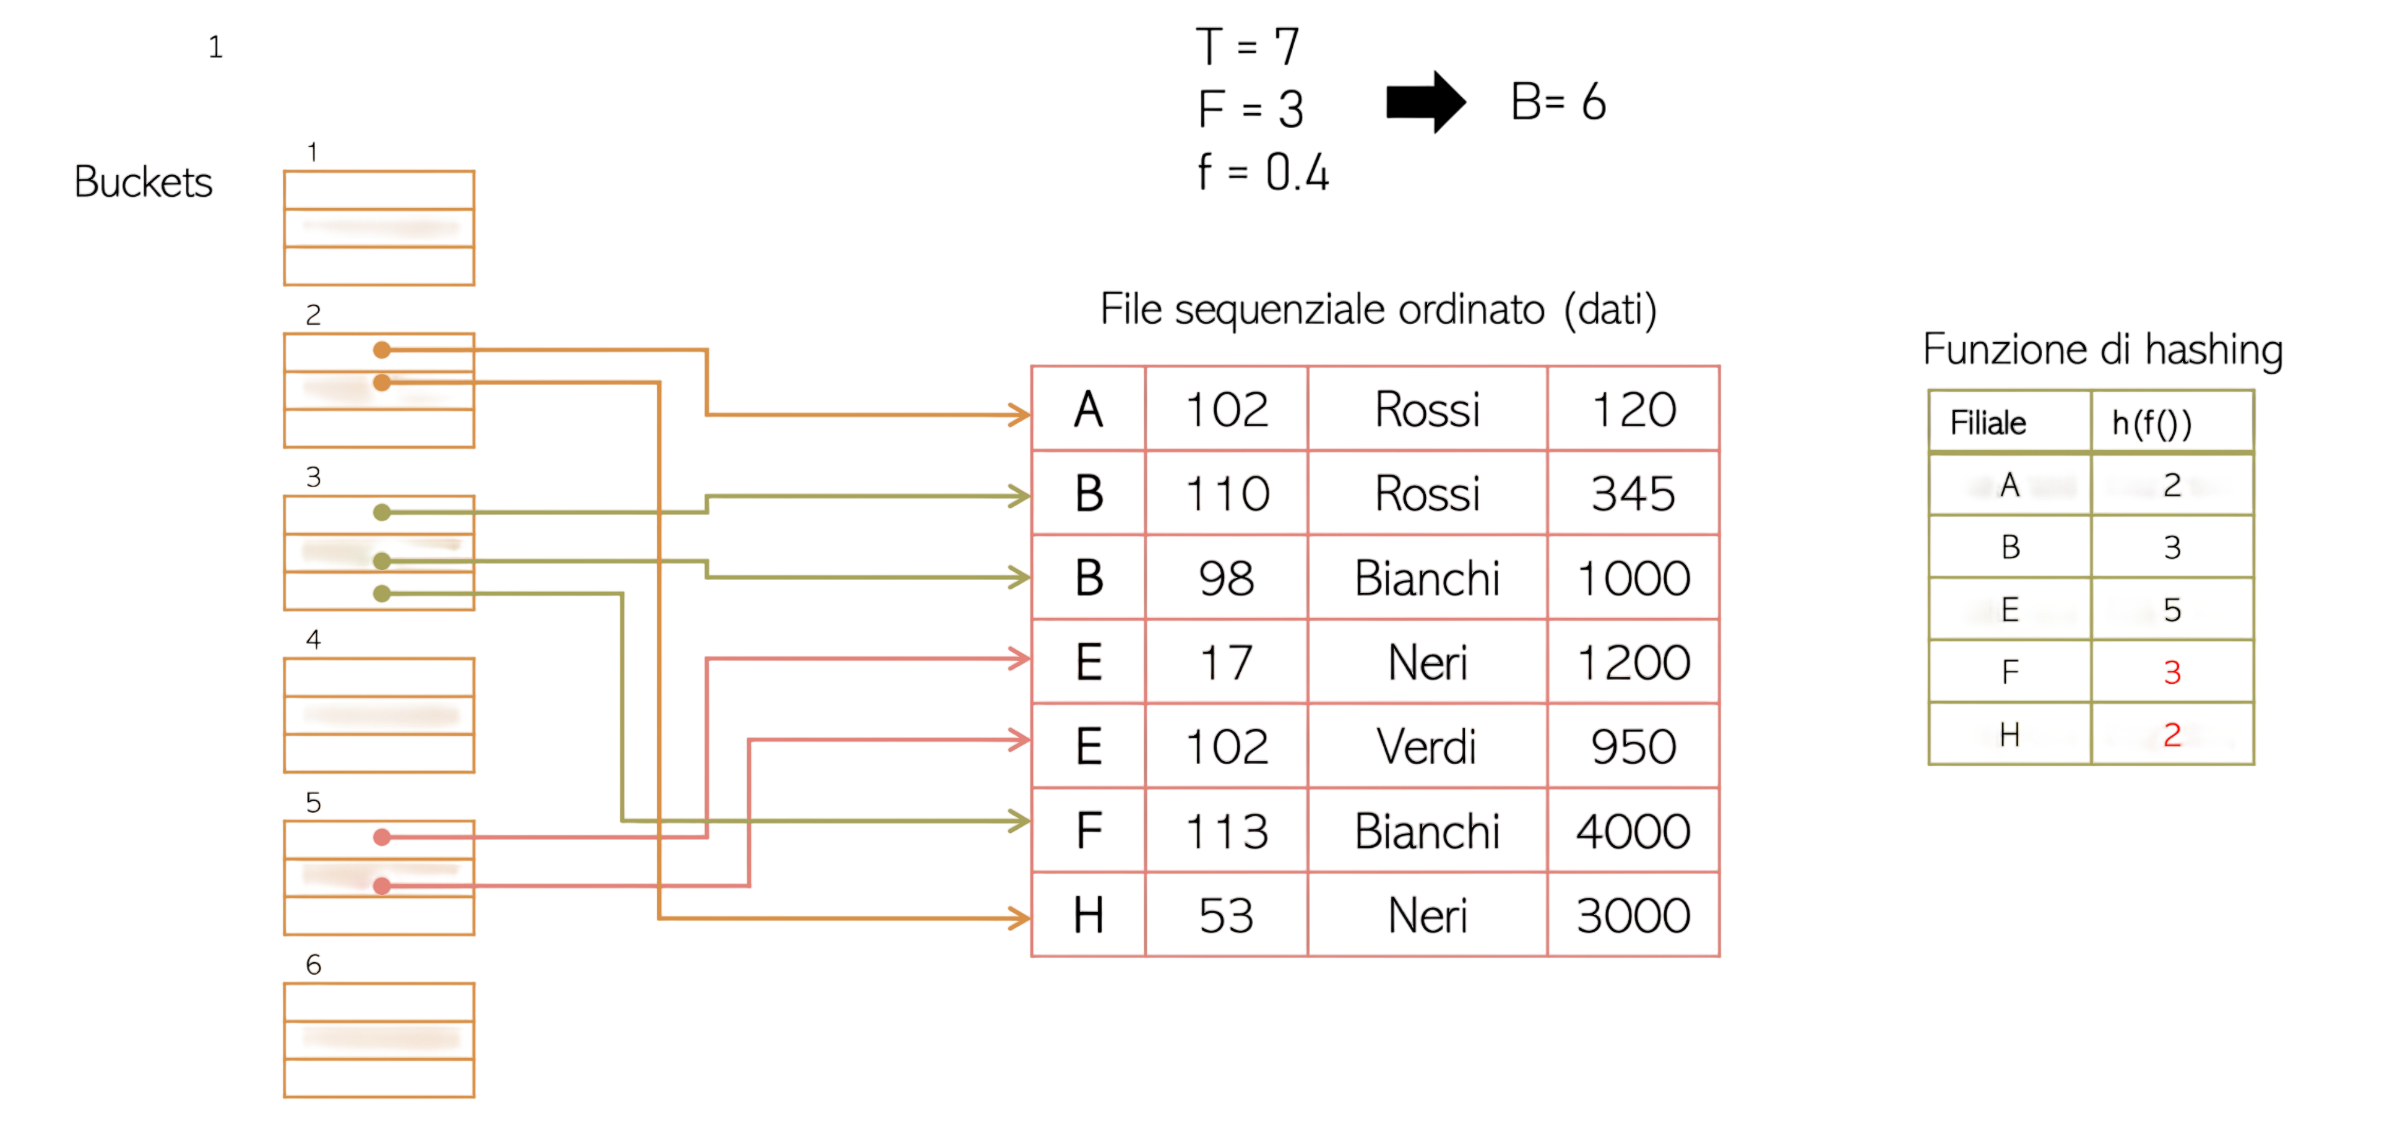
\includegraphics[width=0.9\textwidth]{images/esempio-tabella-hash.png}
  \end{figure}
}

\paragraph{Operazione: ricerca con chiave K}
Per efettuare la ricerca di una tupla con chiave di ricerca K si effettuano i seguenti passi:
\begin{enumerate}[itemsep=\medskipamount]
  \item calcolare $\mathrm{b = h(f(K))}$ (costo zero)
  \item accedere al bucket $\mathrm{b}$ (costo: 1 accesso alla pagina di memoria secondaria)
  \item accedere alle $\mathrm{n}$ tuple attraverso i puntatori del bucket (costo: $\mathrm{m}$ accessi a pagine di memoria secondaria, con $\mathrm{m \leq n}$)
\end{enumerate}

L'inserimento e la cancellazione hanno costo simile alla ricerca.

\paragraph{Collisioni}
La struttura ad accesso calcolato funziona se i buckets conservano un basso coefficiente di riempimento.\\[0.2ex]
Infatti, il problema delle strutture ad accesso calcolato è la gestione delle collisioni.

\definizione{collisione}{
  Una \textbf{collisione} si verifica, quando, dati due valori di chiave $\mathrm{K_1}$ e $\mathrm{K_2}$ con $\mathrm{K_1} \neq \mathrm{K_2}$, risulta:
  \begin{equation*}
    \boldsymbol{\mathrm{h(f(K_1)) = h(f(K_2))}}
  \end{equation*}
}

La probabilità che uno stesso bucket riceva $\mathrm{t}$ chiavi su $\mathrm{n}$ inserimenti è:
\begin{equation*}
  \mathrm{p(t) = \binom{n}{t} \cdot (\frac{1}{B})^t \cdot (1 - \frac{1}{B})^{n - t}}
\end{equation*}

dove:
\begin{itemize}[label=$\triangleright$]
  \item $\mathrm{B}$: numero totale di bucket
\end{itemize}

La probabilità di avere più di $\mathrm{F}$ collisioni, con $\mathrm{F}$ il fattore blocco, cioè il numero di puntatori nel bucket, è:
\begin{equation*}
  \mathrm{p_K = 1 - \sum_{i = 0}^{F}p(i)}
\end{equation*}

\medskip
Un numero ecessivo di collisioni porta alla saturazione del bucket corrispondente.\\[0.2ex]
Per gestirlo si introducono dei \textbf{bucket di overflow} collegati al bucket originale, che contengono i puntatori alle tuple che hanno causato la saturazione del bucket originale.\\[0.2ex]
Le prestazioni della ricerca peggiorano perchè bisogna accedere ai bucket di overflow.

\begin{figure}[H]
  \centering
  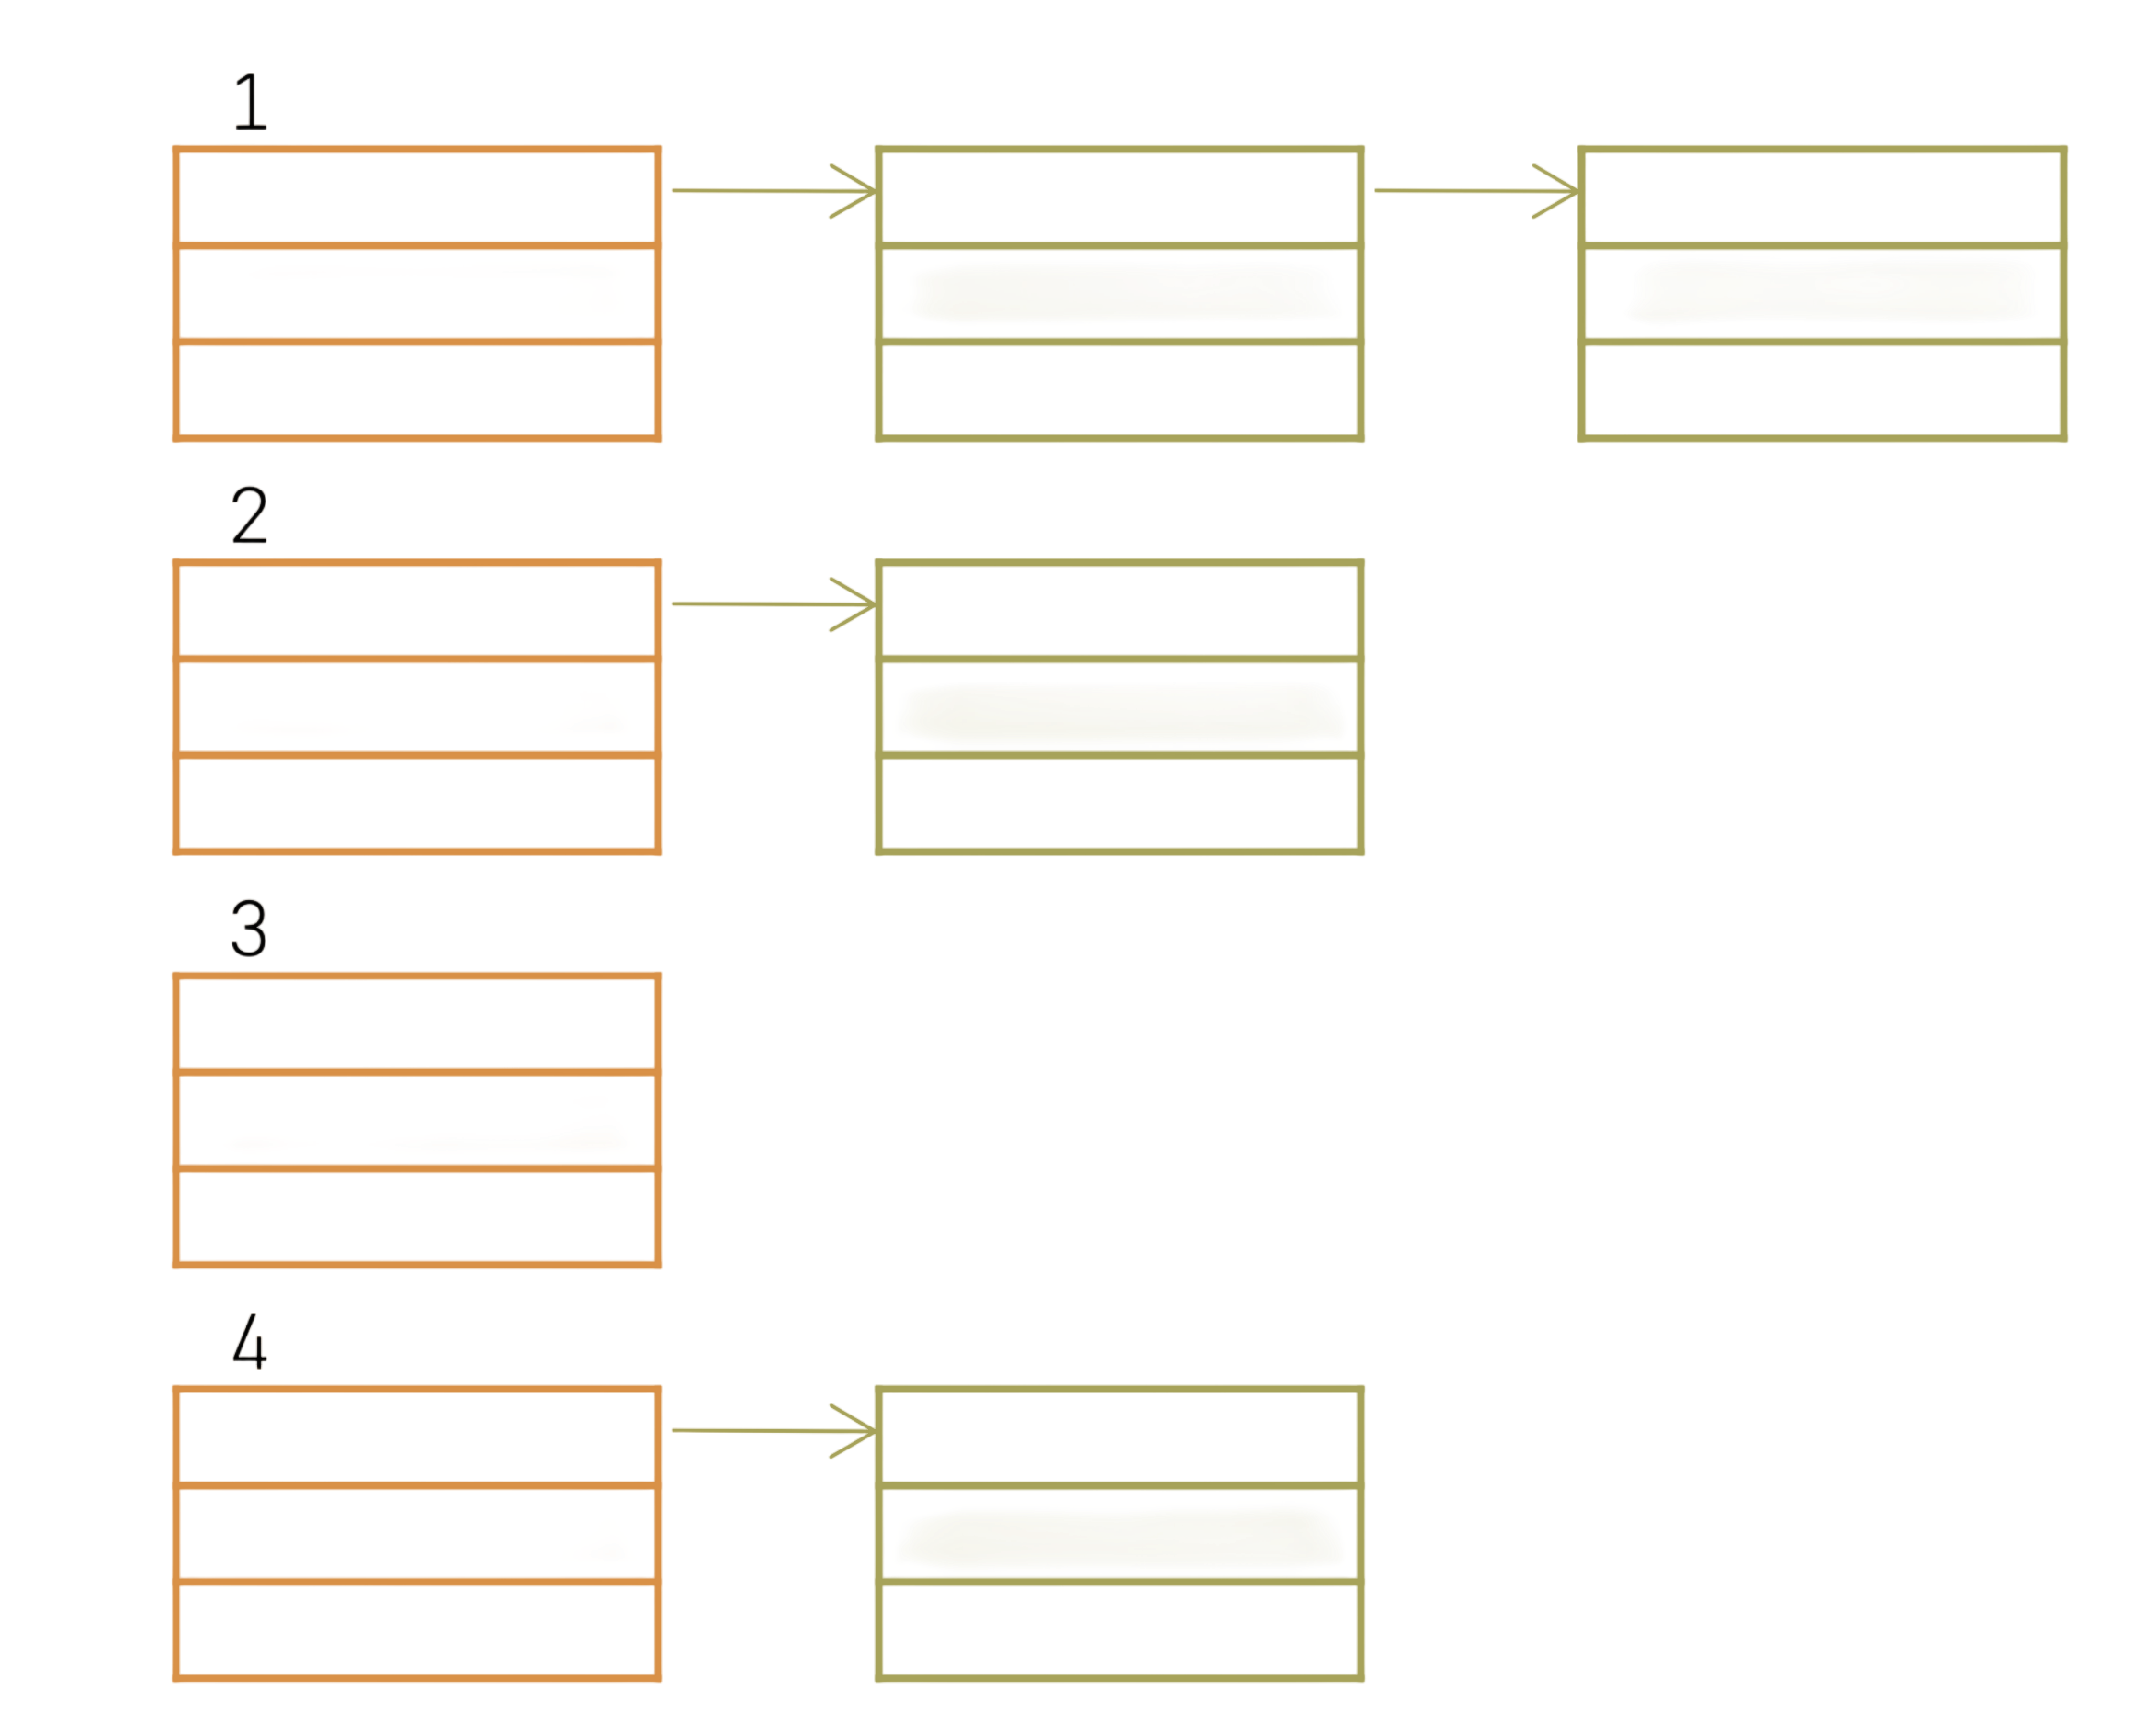
\includegraphics[width=0.5\textwidth]{images/gestione-collisioni-tabella-hash.png}
\end{figure}

    %Tex root = BasiDiDati.tex

\chapter{Esecuzione concorrente di transazioni}
L'unità di misura usata per valutare il carico di lavoro din un DBMS è il \textcolor{azzurrino}{\textbf{numero di transazioni al secondo}} (tps).\\[0.2ex]
Per gestire con prestazioni accettabili il carico di lavoro tipico delle applicazioni gestionali è di 100 o 1000 tps.\\[0.2ex]
L'esecuzione concorrente di transazioni senza controllo può generare \textbf{anomalie} o \textbf{problemi di correttezza}.\\[0.2ex]
Bisogna, quindi, introdurre dei meccanismi di controllo nell'esecuzione delle transazioni per evitare tali anomalie.

\section{Tipologie di anomalie}
Le principali tipologie di anomalie sono:
\begin{itemize}[label=$\triangleright$, itemsep=\smallskipamount]
    \item \textbf{perdita di aggiornamento}: effetti di una transazione concorrente vengono persi (riscritti)
    \item \textbf{lettura inconsistente}: accessi sucessivi alla stessa risorsa ritornano risultati diversi
    \item \textbf{lettura sporca}: viene letto un dato che rappresenta uno stato intermedio di un'altra transazione
    \item \textbf{aggiornamento fantasma}: osservazione di uno stato intermedio che viola i vincoli d'integrità
    \item \textbf{inserimento fantasma}: valutazioni diverse di operazioni di aggregazione producono risultati diversi
\end{itemize}

\vario{Notazione}{
    \begin{itemize}[label=$\diamond$, itemsep=\smallskipamount]
        \item $\mathbf{t_i}$: transazione $\mathrm{t_i}$
        \item $\mathbf{r_i(x)}$: operazione di lettura eseguita dalla transazione $\mathrm{t_i}$ sulla risorsa $\mathrm{x}$
        \item $\mathbf{w_i(x)}$: operazione di scrittura eseguita dalla transazione $\mathrm{t_i}$ sulla risorsa $\mathrm{x}$
    \end{itemize}
}

\subsection{Perdita di aggiornamento}
Nella \textbf{perdita di aggiornamento} gli effetti di una transazione concorrente vengono persi.

\esempio{perdita di aggiornamento}{
    Consieriamo le seguenti transazioni:
    \[
        \begin{aligned}
            \mathrm{t_1}:\; & \texttt{BOT}; \; \mathrm{r_1(x)}; \;\mathrm{ x = x + 1}; \; \mathrm{w_1(x)}; \; \texttt{COMMIT}; \; \texttt{EOT} \\
            \mathrm{t_2}:\; & \texttt{BOT}; \; \mathrm{r_2(x)}; \; \mathrm{x = x + 1}; \; \mathrm{w_2(x)}; \; \texttt{COMMIT}; \; \texttt{EOT}
        \end{aligned}
    \]

    Simuliamo l'esecuzione concorrente di $\mathrm{t_1}$ e $\mathrm{t_2}$:
    \begin{figure}[H]
        \centering
        \includegraphics[width=0.9\textwidth]{images/perdita-aggiornamento.png}
    \end{figure}
}

\subsection{Lettura inconsistente}
Nella \textbf{lettura inconsistente} gli accessi successivi a uno stesso dato all'interno di una transazione ritornano valori diversi.

\esempio{lettura inconsistente}{
    Consieriamo le seguenti transazioni:
    \[
        \begin{aligned}
            \mathrm{t_1}:\; & \texttt{BOT}; \; \mathrm{r_1(x)}; \; \mathrm{r_1'(x)}; \; \texttt{COMMIT}; \; \texttt{EOT} \\
            \mathrm{t_2}:\; & \texttt{BOT}; \; \mathrm{r_2(x)}; \; \mathrm{x = x + 1}; \; \mathrm{w_2(x)}; \; \texttt{COMMIT}; \; \texttt{EOT}
        \end{aligned}
    \]

    Simuliamo l'esecuzione concorrente di $\mathrm{t_1}$ e $\mathrm{t_2}$:
    \begin{figure}[H]
        \centering
        \includegraphics[width=0.9\textwidth]{images/lettura-inconsistente.png}
    \end{figure}
}

\subsection{Lettura sporca}
Nella \textbf{lettura sporca} viene letto un dato che rappresenta uno stato intermedio nell'evoluzione di una transazione.

\esempio{lettura inconsistente}{
    Consieriamo le seguenti transazioni:
    \[
        \begin{aligned}
            \mathrm{t_1}:\; & \texttt{BOT}; \; \mathrm{r_1(x)}; \; \texttt{COMMIT}; \; \texttt{EOT} \\
            \mathrm{t_2}:\; & \texttt{BOT}; \; \mathrm{r_2(x)}; \; \mathrm{x = x + 1}; \; \mathrm{w_2(x)}; \; \dots \texttt{ABORT};
        \end{aligned}
    \]

    Simuliamo l'esecuzione concorrente di $\mathrm{t_1}$ e $\mathrm{t_2}$:
    \begin{figure}[H]
        \centering
        \includegraphics[width=0.9\textwidth]{images/lettura-sporca.png}
    \end{figure}
}

\subsection{Aggiornamento fantasma}
L'\textbf{aggiornamento fantasma} consiste nell'osservazione di uno stato intermedio che non soddisfa i vincoli d'integrità.

\esempio{lettura inconsistente}{
    Consieriamo le seguenti transazioni:
    \[
        \begin{aligned}
        \text{Risorse} &: \mathrm{x, y, z} \\
        \text{Vincoli} &: \mathrm{x + y + z = 100} \\
        \end{aligned}
    \] 
    \[
        \begin{aligned}
        \mathrm{t_1}:\; & \texttt{BOT}; \; \mathrm{r_1(y)}; \; \mathrm{r_1(x)}; \; \mathrm{r_1(z)}; \; \mathrm{s = x + y + z}; \; \texttt{EOT} \\
        \mathrm{t_2}:\; & \texttt{BOT}; \; \mathrm{r_2(y)}; \; \mathrm{y = y + 10}; \; \mathrm{r_2(z)}; \; \mathrm{z = z - 10}; \; \mathrm{w_2(y)}; \; \mathrm{w_2(z)};
        \; \texttt{COMMIT}; \; \texttt{EOT}
        \end{aligned}
    \] 

    Simuliamo l'esecuzione concorrente di $\mathrm{t_1}$ e $\mathrm{t_2}$:
    \begin{figure}[H]
        \centering
        \includegraphics[width=0.9\textwidth]{images/aggiornamento-fantasma.png}
    \end{figure}
}

\subsection{Inserimento fantasma}
L'\textbf{inserimento fantasma} si verifica quando avvengono valutazioni diverse di valori aggregati a causa di inserimenti intermedi.\\[0.2ex]
La transazione che valuta un valore aggregato relativo a tutti gli elementi che soddifano un predicato di selezione (es. voto medio degli studenti) può subire l'anomalia di inserimento se il valore aggregato viene valutato due volte e tra la prima e la seconda valutazione viene inserito un nuovo studente.

\section{Schedule}
\definizione{schedule}{
    Lo \textbf{schedule} è una sequenza di operazioni di lettura e scrittura eseguite su risorse della base di dati da diverse transazioni concorrenti.
}

Lo schedule, quindi, rappresenta una possibile esecuzione concorrente di diverse transazioni:
\begin{equation*}
    \mathbf{S: r_1(x) \quad r_2(x) \quad w_1(z) \quad w_2(x)}
\end{equation*}

Per evitare anomalie, si stabilisce di accettare solo gli schedule equivalenti a uno schedule seriale.

\subsection{Schedule seriale}
\definizione{schedule seriale}{
    Uno \textbf{schedule seriale} è uno schedule dove le operazioni di ogni transazione compaiono un seuqenza senza essere inframezzate da operazioni di altre transazioni.

    \noindent\rule{\textwidth}{0.4pt}

    \medskip
    \[
        \begin{aligned}
            \mathrm{s_1}: \mathrm{r_1(x)} \quad \mathrm{r_2(x)} \quad \mathrm{w_2(x)} \quad \mathrm{w_1(x)} &= \textbf{\text{NON è SERIALE}}\\
            \mathrm{s_2}: \mathrm{r_1(x)} \quad \mathrm{w_1(x)} \quad \mathrm{r_2(x)} \quad \mathrm{w_2(x)} &= \textbf{\text{è SERIALE}}
        \end{aligned}
    \]
}

\definizione{schedule serializzabile}{
    Lo \textbf{schedule serializzabile} è uno schedule equivalente a uno schedule seriale.
}

Due schedule si definiscono equivalenti se \textbf{producono gli stessi effetti} sulla base di dati.

\section{Tecniche di gestione della concorrenza}
Per le seguenti tecniche di gestione della concorrenza, si assume l'ipotesi di \textbf{commit-proiezione} (transazioni hanno esito noto).\\[0.2ex]
Di conseguenza, vengono tolti dagli schedule tutte le operazioni delle transazioni che non vanno a buon fine.

\subsection{View-equivalenza}
\definizione{relazione \texttt{LEGGE\_DA}}{
    Dato uno schedule $\mathrm{S}$, si dice che un'operazione di lettura $\mathrm{r_i(x)}$ (che compare in $\mathrm{S}$) \texttt{LEGGE\_DA} un'operazione di scrittura $\mathrm{w_i(x)}$ (che compare in $\mathrm{S}$), se $\mathrm{w_j(x)}$ \textbf{precede} $\mathrm{r_i(x)}$ in S e non è alcuna operazione $\mathrm{w_k(x)}$ tra le due.

    \[
        \begin{aligned}
            \mathrm{S_1}: \mathrm{r_1(x)} \ \mathrm{r_2(x)} \ \mathrm{w_2(x)} \ \mathrm{w_1(x)} \quad &\texttt{LEGGE\_DA(S1)} = \emptyset\\
            \mathrm{S_2}: \mathrm{r_1(x)} \ \mathrm{w_1(x)} \ \mathrm{r_2(x)} \ \mathrm{w_2(x)} \quad &\texttt{LEGGE\_DA(S2)} = \{(\mathrm{r_2(x), w_1(x)})\}\\
            \mathrm{S_3}: \mathrm{r_1(x)} \ \mathrm{w_1(x)} \ \mathrm{w_2(x)} \ \mathrm{r_2(x)} \quad &\texttt{LEGGE\_DA(S3)} = \emptyset
        \end{aligned}
    \]
}

\definizione{scritture finali}{
    Dato uno schedule $\mathrm{S}$ si dice che un'operazione di scrittura $\mathrm{w_i(x)}$ (che compare in $\mathrm{S}$) è una \texttt{scrittura finale} se è l'ultima operazione di scrittura della risorsa $\mathrm{x}$ in $\mathrm{S}$.

    \[
       \begin{aligned}
            \mathrm{S_1}: \mathrm{r_1(x)} \ \mathrm{r_2(x)} \ \mathrm{w_2(x)} \ \mathrm{w_3(y)} \ \mathrm{w_1(x)} \quad &\texttt{SCRITTURE\_FINALI(S1)} = \{\mathrm{w_3(y)}, \mathrm{w_1(x)}\}\\
            \mathrm{S_2}: \mathrm{r_1(x)} \ \mathrm{w_1(x)} \ \mathrm{r_2(x)} \ \mathrm{w_2(x)} \ \mathrm{w_3(y)} \quad &\texttt{SCRITTURE\_FINALI(S1)} = \{\mathrm{w_2(x), w_3(y)}\}
        \end{aligned}     
    \]
}

\definizione{view-equivalenza}{
    Due schedule $\mathrm{S_1}$ e $\mathrm{S_2}$ sono \textbf{view-equivalenti} $(\mathbf{S_1} \ \mathbf{\approx_V} \ \mathbf{S_2})$ se possiedono le stesse relazioni \texttt{LEGGE\_DA} e \texttt{SCRITTURE\_FINALI}.
}

\definizione{viwe-serializzabilità}{
    Uno schedule S è \textbf{view-serializzabili} (VSR) se esiste uno schedule seriale $\mathrm{S'}$ tale che $\mathbf{S \ \approx_V \ S'}$.

    \vario{Attenzione}{
        Gli schedule seriali $\mathrm{S'}$ si generano considerando tutte le possibili permutazioni delle transazioni (non delle operazioni delle transazioni) che compaiono in $\mathrm{S}$.

        Inoltre, non si deve cambiare l'ordine delle operazioni di ciascuna transazione perchè ciò significherebbe modificare la transazione.
    }
}

Gli schedule corrispondenti alle anomalie di:
\begin{itemize}[label=$\diamond$, itemsep=\smallskipamount]
    \item perdita di aggiornamento
    \item letture inconsistenti
    \item aggiornamenti fantasmi
\end{itemize}

non sono view-serializzabili.\\[0.2ex]
Inoltre, l'algoritmo per il test di view-equivalenza tra due schedule è di complessità lineare, mentre per il test di view-serializzabilità di uno schedule è di complessità esponenziale.\\[0.2ex]
In conclusione si è osservato che la view-serializzabilità richiede l'ipotesi di commit-proiezione e algoritmi di complessità troppo elevata, quindi, non è applicabile nei sistemi reali.

\esercizio{perdita di aggiornamento}{
    Consideriamo le seguenti transazioni:
  \[
  \begin{aligned}
    \mathrm{t_1}:\; & \mathrm{r_1(x)}; \; \mathrm{w_1(x)} \\
    \mathrm{t_2}:\; & \mathrm{r_2(x)}; \; \mathrm{w_2(x)}
  \end{aligned}
  \] 
  Eseguire lo schedule:
  \[
    \mathbf{S_{pa} = r_1(x); \; r_2(x); \; w_2(x); \; w_1(x);}
  \]

  \textcolor{red}{\textbf{Questo schedule è view serializzabile?}}

  \smallskip
  Calcoliamo le relazioni:
  \begin{itemize}[label=$\triangleright$, itemsep=\smallskipamount]
    \item \texttt{LEGGE\_DA}\( (\mathrm{S_{pa}}) = \varnothing \)
    \item \texttt{SCRITTURE\_FINALI}\( (\mathrm{S_{pa}}) = \{ \mathrm{w_1(x)} \} \)
  \end{itemize}

  \smallskip
  Bisogna generare tutti i possibili schedule seriali per determinare se
  esiste uno schedule seriale \( \mathrm{S'} \) tale che \( \mathrm{S_{pa} \approx_V S'} \).

  Gli schedule seriali sono:
  \begin{itemize}[label=$\circ$, itemsep=\medskipamount]
    \item \( \mathbf{S_{12} = r_1(x); \; w_1(x); \; r_2(x); \; w_2(x);} \) 
      \begin{itemize}[itemsep=\smallskipamount]
        \item \texttt{LEGGE\_DA}\( \mathrm{(S_{12})} = \{ \mathrm{(r_2(x), w_1(x))} \} \)
        \item \texttt{SCRITTURE\_FINALI}\( \mathnormal{(S_{12})} = \{ \mathrm{w_1(x)} \} \)
      \end{itemize}
      Osserviamo che \( \mathbf{S_{pa} \not\approx_V S_{12}} \)

    \item \( \mathbf{S_{21} = r_2(x); \; w_2(x); \; r_1(x); \; w_1(x);} \) 
      \begin{itemize}[itemsep=\smallskipamount]
        \item \texttt{LEGGE\_DA}\( \mathrm{(S_{21})} = \{ \mathrm{(r_1(x), w_2(x))} \} \)
        \item \texttt{SCRITTURE\_FINALI}\( \mathrm{(S_{21})} = \{ \mathrm{w_1(x)} \} \)
      \end{itemize}
      Osserviamo che \( \mathbf{S_{pa} \not\approx_V S_{21}} \)
  \end{itemize}

  \smallskip
  Avendo provato per tutte le possibili permutazioni si può dire che lo schedule
  \( \mathrm{S_{pa}} \) \textbf{non è view-serializzabile}.
}

\esercizio{lettura inconsistente}{
    Consideriamo le seguenti transazioni:
  \[
  \begin{aligned}
    \mathrm{t_1}:\; & \mathrm{r_1(x)}; \; \mathrm{w_1(x)}; \; \mathrm{r_1(y)}; \; \mathrm{w_1(y)} \\
    \mathrm{t_2}:\; & \mathrm{r_2(z)}; \; \mathrm{r_2(x)}; \; \mathrm{w_2(x)}; \; \mathrm{w_2(z)}
  \end{aligned}
  \]

  Eseguire lo schedule:
  \[
    \mathbf{S_1 = r_1(x); \; w_1(x); \; r_2(z); \; r_1(y); \; w_1(y); \; r_2(x); \; w_2(x); \;
    w_2(z);}
  \]

  \textcolor{red}{\textbf{Questo schedule è view serializzabile?}}

  \smallskip
  Calcoliamo le relazioni:
  \begin{itemize}[label=$\triangleright$, itemsep=\smallskipamount]
    \item \texttt{LEGGE\_DA}\( \mathrm{(S_1)} = \left\{ \mathrm{(r_2(x), w_1(x))} \right\} \)
    \item \texttt{SCRITTURE\_FINALI}\( \mathrm{(S_1)} = \left\{ \mathrm{w_2(x), w_1(y), w_2(z)} \right\} \)
  \end{itemize}

  \smallskip
  Bisogna generare tutti i possibili schedule seriali per determinare se
  esiste uno schedule seriale \( \mathrm{S'} \) tale che \( \mathrm{S_1 \approx_V S'} \).

  Gli schedule seriali sono:
  \begin{itemize}[label=$\circ$, itemsep=\medskipamount]
    \item \( \mathbf{S_{12} = t_1 t_2} \) 

    \item \( \mathbf{S_{21} = t_2 t_1} \) 
  \end{itemize}

  \smallskip
  Al posto di creare tutte le permutazioni degli schedule seriali, cerchiamo di
  osservare le relazioni \texttt{LEGGE\_DA} e \texttt{SCRITTURE\_FINALI} per capire se \( \mathrm{S_1} \) è view-equivalente ad \( \mathrm{S_{12}} \) o \( \mathrm{S_{21}} \).

  Dalla presenza di \( \mathrm{w_2(x)} \) nelle scritture finali di \( \mathrm{S_1} \) si nota che
  \( \mathrm{t_1 < t_2} \) perchè \( \mathrm{w_2(x)} \) è l'ultima scrittura di \( \mathrm{x} \) in \( \mathrm{S_1} \), 
  e questa operazione viene eseguita solo da \( \mathrm{t_2} \) e di conseguenza va eseguita
  dopo \( \mathrm{t_1} \). Da ciò sappiamo che sicuramente \( \mathrm{S_1 \not\approx_V S_{21}} \) e ci rimane da controllare soltanto se \( \mathrm{S_1 \approx_V S_{12}} \):
  \[
    \mathbf{S_{12} = r_1(x); \; w_1(x); \; r_1(y); \; w_1(y); \; r_2(z); \; r_2(x); \; w_2(x); \;
    w_2(z);}
  \] 
  \begin{itemize}[label=$\triangleright$, itemsep=\smallskipamount]
    \item \texttt{LEGGE\_DA}\( \mathrm{(S_{12})} = \left\{ \mathrm{(r_2(x), w_1(x))} \right\} \)
    \item \texttt{SCRITTURE\_FINALI}\( \mathrm{(S_{12})} = \left\{ \mathrm{w_2(x), w_1(y), w_2(z)} \right\} \)
  \end{itemize}

  \smallskip
  Osserviamo che \( \mathrm{S_1 \approx_V S_{12}} \) e quindi \( \mathrm{S_1} \) è \textbf{view-serializzabile}.
}

\esercizio{}{
    Consideriamo le seguenti transazioni:
  \[
  \begin{aligned}
    \mathrm{t_1}:\; & \mathrm{r_1(x)}; \; \mathrm{w_1(x)}; \; \mathrm{r_1(y)}; \; \mathrm{w_1(y)} \\
    \mathrm{t_2}:\; & \mathrm{r_2(z)}; \; \mathrm{r_2(x)}; \; \mathrm{w_2(x)}; \; \mathrm{w_2(z)}
  \end{aligned}
  \]

  Eseguire lo schedule:
  \[
    \mathbf{S_1 = r_1(x); \; w_1(x); \; r_2(z); \; r_1(y); \; w_1(y); \; r_2(x); \; w_2(x); \;
    w_2(z);}
  \]

  \textcolor{red}{\textbf{Questo schedule è view serializzabile?}}

  \smallskip
  Calcoliamo le relazioni:
  \begin{itemize}[label=$\triangleright$, itemsep=\smallskipamount]
    \item \texttt{LEGGE\_DA}\( \mathrm{(S_1)} = \left\{ \mathrm{(r_2(x), w_1(x))} \right\} \)
    \item \texttt{SCRITTURE\_FINALI}\( \mathrm{(S_1)} = \left\{ \mathrm{w_2(x), w_1(y), w_2(z)} \right\} \)
  \end{itemize}

  \smallskip
  Bisogna generare tutti i possibili schedule seriali per determinare se esiste uno schedule seriale \( \mathrm{S'} \) tale che \( \mathrm{S_1 \approx_V S'} \).

  Gli schedule seriali sono:
  \begin{itemize}[label=$\circ$, itemsep=\medskipamount]
    \item \( \mathbf{S_{12} = t_1 t_2} \) 

    \item \( \mathbf{S_{21} = t_2 t_1} \) 
  \end{itemize}

  \smallskip
  Al posto di creare tutte le permutazioni degli schedule seriali, cerchiamo di
  osservare le relazioni \texttt{LEGGE\_DA} e \texttt{SCRITTURE\_FINALI} per capire se \( \mathrm{S_1} \) è view-equivalente ad \( \mathrm{S_{12}} \) o \( \mathrm{S_{21}} \).

  Dalla presenza di \( \mathrm{w_2(x)} \) nelle scritture finali di \( \mathrm{S_1} \) si nota che \( \mathrm{t_1 < t_2} \) perchè \( \mathrm{w_2(x)} \) è l'ultima scrittura di \( \mathrm{x} \) in \( \mathrm{S_1} \) e questa operazione viene eseguita solo da \( \mathrm{t_2} \) e di conseguenza va eseguita dopo \( \mathrm{t_1} \).
  
  Da ciò sappiamo che sicuramente \( \mathrm{S_1 \not\approx_V S_{21}} \) e ci rimane da controllare soltanto se \( \mathrm{S_1 \approx_V S_{12}} \):
  \[
    \mathbf{S_{12} = r_1(x); \; w_1(x); \; r_1(y); \; w_1(y); \; r_2(z); \; r_2(x); \; w_2(x); \;
    w_2(z)};
  \]
  \begin{itemize}
    \item \texttt{LEGGE\_DA}\( \mathrm{(S_{12})} = \left\{ \mathrm{(r_2(x), w_1(x))} \right\} \)
    \item \texttt{SCRITTURE\_FINALI}\( \mathrm{(S_{12})} = \left\{ \mathrm{w_2(x), w_1(y), w_2(z)} \right\} \)
  \end{itemize}

  \smallskip
  Osserviamo che \( \mathrm{S_1 \approx_V S_{12}} \) e quindi \( \mathrm{S_1} \) è \textbf{view-serializzabile}.
}

\esercizio{view-serializzabilità}{
  Consideriamo le seguenti transazioni:
  \[
    \begin{aligned}
      \mathrm{t_1}:\; & \mathrm{r_1(x)}; \; \mathrm{w_1(x)}; \; \mathrm{w_1(y)} \\
      \mathrm{t_2}:\; & \mathrm{r_2(y)}; \; \mathrm{r_2(x)} \\
      \mathrm{t_3}:\; & \mathrm{w_3(x)}; \; \mathrm{r_3(y)}; \; \mathrm{w_3(y)}
    \end{aligned}
  \]

  Eseguire lo schedule:
  \[
    \mathbf{S_2 = r_1(x); \; w_1(x); \; w_3(x); \; r_2(y); \; r_3(y); \; w_3(y); \; w_1(y); \;
    r_2(x)}
  \]

  \textcolor{red}{\textbf{Questo schedule è view serializzabile?}}

  \smallskip
  Calcoliamo le relazioni:
  \begin{itemize}[label=$\triangleright$, itemsep=\smallskipamount]
    \item \texttt{LEGGE\_DA}\( \mathrm{(S_2)} = \left\{ \mathrm{(r_2(x), w_3(x))} \right\} \)
    \item \texttt{SCRITTURE\_FINALI}\( \mathrm{(S_2)} = \left\{ \mathrm{w_3(x), w_1(y)} \right\} \)
  \end{itemize}

  \smallskip
  Siccome ci sono 6 possibili permutazioni vediamo se è possibile scartarne alcune
  a priori.
  \begin{itemize}[label=$\circ$, itemsep=\medskipamount]
    \item insieme \texttt{SCRITTURE\_FINALI}\( \mathrm{(S_2)} \) implica:
      \begin{itemize}[itemsep=\smallskipamount]
        \item \( \mathrm{t_1 < t_3} \) perchè \( \mathrm{w_3(x)} \) è l'ultima scrittura di \( \mathrm{x} \) in \( \mathrm{S_2} \) e questa operazione viene eseguita solo da \( \mathrm{t_3} \) e di conseguenza va eseguita dopo \( \mathrm{t_1} \)

        \item \( \mathrm{t_3 < t_1} \) perchè \( \mathrm{w_1(y)} \) è l'ultima scrittura di \( \mathrm{s} \) in \( \mathrm{S_2} \) e questa operazione viene eseguita solo da \( \mathrm{t_1} \) e di conseguenza va eseguita dopo \( \mathrm{t_3} \)
      \end{itemize}
      Si osserva che \( \mathrm{t_1 < t_3} \) e \( \mathrm{t_3 < t_1} \) è una contraddizione, cioè non esiste uno schedule seriale che le rispetti entrambe e quindi si può concludere che \( \mathrm{S_2} \) \textbf{non è view-serializzabile}.

    \item insieme \texttt{LEGGE\_DA}\( \mathrm{(S_2)} \) implica:
      \begin{itemize}[itemsep=\smallskipamount]
        \item \( \mathrm{t_3 < t_2} \) perchè \( \mathrm{r_2(x)} \) (in \( \mathrm{t_2} \)) legge da \( \mathrm{w_3(x)} \) (in \( \mathrm{t_3} \)) e quindi \( \mathrm{(r_2(x), w_3(x))} \in \texttt{LEGGE\_DA} \) 

        \item \( \mathrm{t_1 < t_3} \) per garantire \( \mathrm{(r_1(x), w_3(x))} \notin \texttt{LEGGE\_DA} \)
        \item \( \mathrm{t_2 < t_3} \) per garantire \( \mathrm{(r_2(x), w_3(x))} \in \texttt{LEGGE\_DA} \)
        \item \( \mathrm{t_2 < t_1} \) per garantire \( \mathrm{(r_2(x), w_1(x))} \notin \texttt{LEGGE\_DA} \)
        \item \( \mathrm{t_3 < t_1} \) per garantire \( \mathrm{(r_3(x), w_1(x))} \notin \texttt{LEGGE\_DA} \)
      \end{itemize}

      \smallskip
      Si osserva che \( \mathrm{t_1 < t_3} \) e \( \mathrm{t_3 < t_1} \) è una contraddizione, quindi, si può concludere che \( \mathrm{S_2} \) \textbf{non è view-serializzabile}.
  \end{itemize}
}

\esercizio{view-serializzabilità}{
  Consideriamo le seguenti transazioni:
  \[
    \begin{aligned}
      \mathrm{t_1}:\; & \mathrm{r_1(x)}; \; \mathrm{w_1(x)}; \; \mathrm{w_1(y)}; \; \mathrm{w_1(z)} \\
      \mathrm{t_2}:\; & \mathrm{r_2(x)}; \; \mathrm{w_2(x)} \\
      \mathrm{t_3}:\; & \mathrm{r_3(x)}; \; \mathrm{w_3(y)}; \; \mathrm{w_3(x)} \\
      \mathrm{t_4}:\; & \mathrm{r_4(z)} \\
      \mathrm{t_5}:\; & \mathrm{w_5(x)}; \; \mathrm{w_5(y)}; \; \mathrm{r_5(z)}
    \end{aligned}
  \]

  Eseguire con lo schedule:
  \[
    \begin{aligned}
      S_3 =& r_1(x); \; r_2(x); \; w_2(x); \; r_3(x); \; r_4(z); \; w_1(x); \; w_3(y); \;
      w_3(x); \; w_1(y); \\
          &\; w_5(x); \; w_1(z); \; w_5(y); \; r_5(z)
    \end{aligned}
  \]

  \textcolor{red}{\textbf{Questo schedule è view serializzabile?}}

  \smallskip
  Calcoliamo le relazioni:
  \begin{itemize}[label=$\triangleright$, itemsep=\smallskipamount]
    \item \texttt{LEGGE\_DA}\( (\mathrm{S_3}) = \left\{ \mathrm{(r_3(x), w_2(x)), (r_5(z), w_1(z))} \right\} \)
    \item \texttt{SCRITTURE\_FINALI}\( (\mathrm{S_3}) = \left\{ \mathrm{w_5(x), w_5(y), w_1(z)} \right\} \)
  \end{itemize}

  \smallskip
  Le permutazioni di tutte le transazioni sono \( 5! \) e, quindi, è necessario cercare
  di scartarne alcune:
  \begin{itemize}[label=$\circ$, itemsep=\medskipamount]
    \item Considerando \texttt{SCRITTURE\_FINALI}\( (\mathrm{S_3}) \) si ha che:
      \begin{itemize}[itemsep=\smallskipamount]
        \item \( \mathrm{w_5(x)} \Rightarrow \mathrm{t_2 < t_5,\; t_1 < t_5,\; t_3 < t_5} \) 
        \item \( \mathrm{w_5(y)} \Rightarrow \mathrm{t_3 < t_5,\; t_1 < t_5}\) 
      \end{itemize}
      Da queste informazioni non si rilevano contraddizioni, quindi, si procede con
      l'analisi di \texttt{LEGGE\_DA}\( (S_3) \).

    \item Considerando \texttt{LEGGE\_DA}\( (S_3) \) si ha che:
      \begin{itemize}[itemsep=\smallskipamount]
        \item \( \mathrm{(r_3(x), w_2(x))} \Rightarrow \mathrm{t_2 < t_3} \)
        \item \( \mathrm{(r_5(z), w_1(z))} \Rightarrow \mathrm{t_1 < t_5} \)
      \end{itemize}
      Da queste informazioni non si rilevano contraddizioni, quindi, si procede
      osservando cosa \textbf{non compare} nell'insieme \texttt{LEGGE\_DA}\( (\mathrm{S_3}) \):
      \begin{itemize}[itemsep=\smallskipamount]
        \item \( \mathrm{(r_1(x), w_2(x))} \notin \texttt{LEGGE\_DA}(\mathrm{S_3}) \Rightarrow
           \mathrm{t_1 < t_2} \)

         \item \( \mathrm{(r_1(x), w_3(x))} \notin \texttt{LEGGE\_DA}(\mathrm{S_3}) \Rightarrow
           \mathrm{t_1 < t_3} \)

         \item \( \mathrm{(r_1(x), w_5(x))} \notin \texttt{LEGGE\_DA}\mathrm{(S_3)} \Rightarrow
           \mathrm{t_1 < t_5} \)

         \item \( \mathrm{(r_2(x), w_1(x))} \notin \texttt{LEGGE\_DA}\mathrm{(S_3)} \Rightarrow
           \mathrm{t_2 < t_1} \)
       \end{itemize}
  \end{itemize}

  \smallskip
  Questo è in contraddizione con \( \mathrm{t_1 < t_2} \) e si può concludere che \( \mathrm{S_3} \) \textbf{non è view-serializzabile}.
}

\subsection{Conflict-equivalenza}
\definizione{conflitto}{
    Dato uno schedule $\mathrm{S}$, si dice che una coppia di operazioni $\mathrm{(a_i, a_j)}$, dove $\mathrm{a_i}$ e $\mathrm{a_j}$ compaiono nello schedule $\mathrm{S}$, rappresentano un conflitto se:
    \begin{itemize}[label=$\circ$, itemsep=\smallskipamount]
        \item appartengono a transazioni diverse $\mathrm{(i \neq j)}$
        \item entrambe operano sulla stessa risorsa
        \item almeno una di esse è un'operazione di scrittura
        \item $\mathrm{a_i}$ comapare in $\mathrm{S}$ prima di $\mathrm{a_j}$
    \end{itemize}
}

\definizione{conflit-equivalenza}{
    Due schedule $\mathrm{S_1}$ e $\mathrm{S_2}$ sono \textbf{conflit-equivalenti} ($\mathbf{S_1 \ \approx_C \ S_2}$) se possiedono le stesse operazioni e gli stessi conflitti, cioè se le operazioni in conflitto sono nello stesso ordine nei due schedule.
}

\definizione{conflict-serializzabile}{
    Uno schedule $\mathrm{S}$ è \textbf{conflit-serializzabile} (CSR) se esiste uno schedule seriale $\mathrm{S'}$ tale che $\mathrm{S \ \approx_C \ S'}$.
}

L'algoritmo per il test di conflit-serializzabilità di uno schedule è di complessità linerare.

\smallskip
Dato il seguente schedule $\mathrm{S}$:
\begin{itemize}[label=$\diamond$, itemsep=\smallskipamount]
    \item si costruisce il grafo dei conflitti $\mathrm{G(N,A)}$ dove:
    \begin{itemize}[label=$\triangleright$, itemsep=\smallskipamount]
        \item $\mathrm{N = t_1 \dots t_n}$: insieme delle transazioni di $\mathrm{S}$
        \item $\mathrm{(t_i, t_j) \in A}$ se esiste almeno un conflitto ($\mathrm{a_i, a_j}$) in $\mathrm{S}$
    \end{itemize}
    \item \textbf{se il grafo è aciclico} $\Rightarrow \mathbf{S}$ \textbf{è conflit-serializzabile}
    
    \vario{Dimostrazione}{
        \begin{enumerate}[itemsep=\medskipamount]
            \item se $\mathrm{S}$ è CSR, cioè esiste uno schdeule $\mathrm{S_R}$ seriale tale che $\mathrm{S \ \approx_C S_r}$, allora il suo grafo è aciclico.
            
            \smallskip
            \textbf{Ipotesi}: le transazioni di $\mathrm{S_r}$ sono ordinate:
            \[
                \mathrm{t_1, t_2, \dots, t_n}
            \]

            Poichè $\mathrm{S \ \approx_C S_r}$, allora $\mathrm{S_r}$ ha tutti i conflitti di $\mathrm{S}$ con operazioni esattamente nello stesso ordine.

            Quindi nel grafo dei conflitti di $\mathrm{S_r}$, ci possono essere solo archi ($\mathrm{i,j}$) con $\mathrm{i<j}$ e, questo, vuol dire che non possono esserci cicli poichè un ciclo richiederebbe un arco ($\mathrm{i,j}$) con $\mathrm{j > i}$ che è impossibile.

            Siccome $\mathrm{S \ \approx_C S_r}$, allora hanno lo stesso grafo dei conflitti e, quindi, anche il grafo dei conflitti di $\mathrm{S}$ è aciclico.
            \item se il grafo $\mathrm{S}$ è aciclico, allora $\mathrm{S}$ è CSR cioè esiste uno schdeule $\mathrm{S_R}$ seriale tale che $\mathrm{S \ \approx_C S_r}$ e, quindi, $\mathrm{S}$ e $\mathrm{S_R}$ hanno gli stessi conflitti e, quindi, lo stesso grafo.
            
            \smallskip
            \textbf{Ipotesi}: il grafo dei conflitti di $\mathrm{S}$ è aciclico e, quindi, esiste un ordinamento topologico, cioè un'enumerazione dei nodi tale che il garfo contiene solo archi ($\mathrm{i, j}$) con $\mathrm{i < j}$.

            Utilizzando questo ordinamento toplogico possiamo definire un ordine delle transazioni che produce lo stesso grafo e, quindi, siccome le transazioni sono ordinate si ha uno schdeule seriale.
        \end{enumerate}
    }
\end{itemize}

Richede comunque l'ipotesi di commit-proiezione.

\esempio{perdita di aggiornamento}{
    Consideriamo le seguenti transazioni:
  \[
    \begin{aligned}
      \mathrm{t_1}:\; & \mathrm{r_1(x)}; \; \mathrm{w_1(x)} \\
      \mathrm{t_2}:\; & \mathrm{r_2(x)}; \; \mathrm{w_2(x)}
    \end{aligned}
  \]

  Eseguire lo schedule:
  \[
    \mathbf{S_{pa}:\; r_1(x); \; r_2(x); \; w_2(x); \; w_1(x);}
  \]

  \smallskip
  L'insieme dei conflitti è:
  \[
    CONFLITTI(\mathrm{S_{pa}}) = \left\{ (\mathrm{r_1(x), w_2(x)),\; (r_2(x), w_1(x)),\; (w_2(x), w_1(x)}) \right\}
  \]

  Generiamo il grafo dei conflitti:
  \begin{figure}[H]
    \centering
    \begin{tikzpicture}
      \node[circle, draw] (t1) at (0,0) {\( t_1 \)};
      \node[circle, draw] (t2) at (3,0) {\( t_2 \)};

      \draw[->] (t1) edge [bend left] node[above] {\( r_1(x), w_2(x) \)} (t2);
      \draw[->] (t2) edge [bend left] node[below] {\( r_2(x), w_1(x) \)} (t1);
    \end{tikzpicture}
  \end{figure}

  \smallskip
  Siccome il grafo ha un ciclo \( \mathrm{S_{pa}} \) \textbf{non è conflict-serializzabile}.
}

\esempio{lettura inconsistente}{
    Consideriamo le seguenti transazioni:
  \[
    \begin{aligned}
      \mathrm{t_1}:\; & \mathrm{r_1(x)}; \; \mathrm{r'_1(x)} \\
      \mathrm{t_2}:\; & \mathrm{r_2(x)}; \; \mathrm{w_2(x)}
    \end{aligned}
  \]

  Eseguire lo schedule:
  \[
    \mathbf{S_{pa}:\; r_1(x); \; r_2(x); \; w_2(x); \; r'_1(x);}
  \]

  \smallskip
  L'insieme dei conflitti è:
  \[
    CONFLITTI(\mathrm{S_{pa}}) = \left\{ (\mathrm{r_1(x), w_2(x)),\; (w_2(x), r'_1(x)}) \right\}
  \]

  Generiamo il grafo dei conflitti:
  \begin{figure}[H]
    \centering
    \begin{tikzpicture}
      \node[circle, draw] (t1) at (0,0) {\( t_1 \)};
      \node[circle, draw] (t2) at (3,0) {\( t_2 \)};

      \draw[->] (t1) edge [bend left] node[above] {\( r_1(x), w_2(x) \)} (t2);
      \draw[->] (t2) edge [bend left] node[below] {\( w_2(x), r'_1(x) \)} (t1);
    \end{tikzpicture}
  \end{figure}
}

\teorema{conflict-serializzabile}{
    La conflict-serializzabilità è una condizione sufficiente, ma non necessaria per la view-serializzabilità, cioè:
    \[
        \mathrm{CSR \subset VSR}
    \]

    \begin{figure}[H]
     \centering
     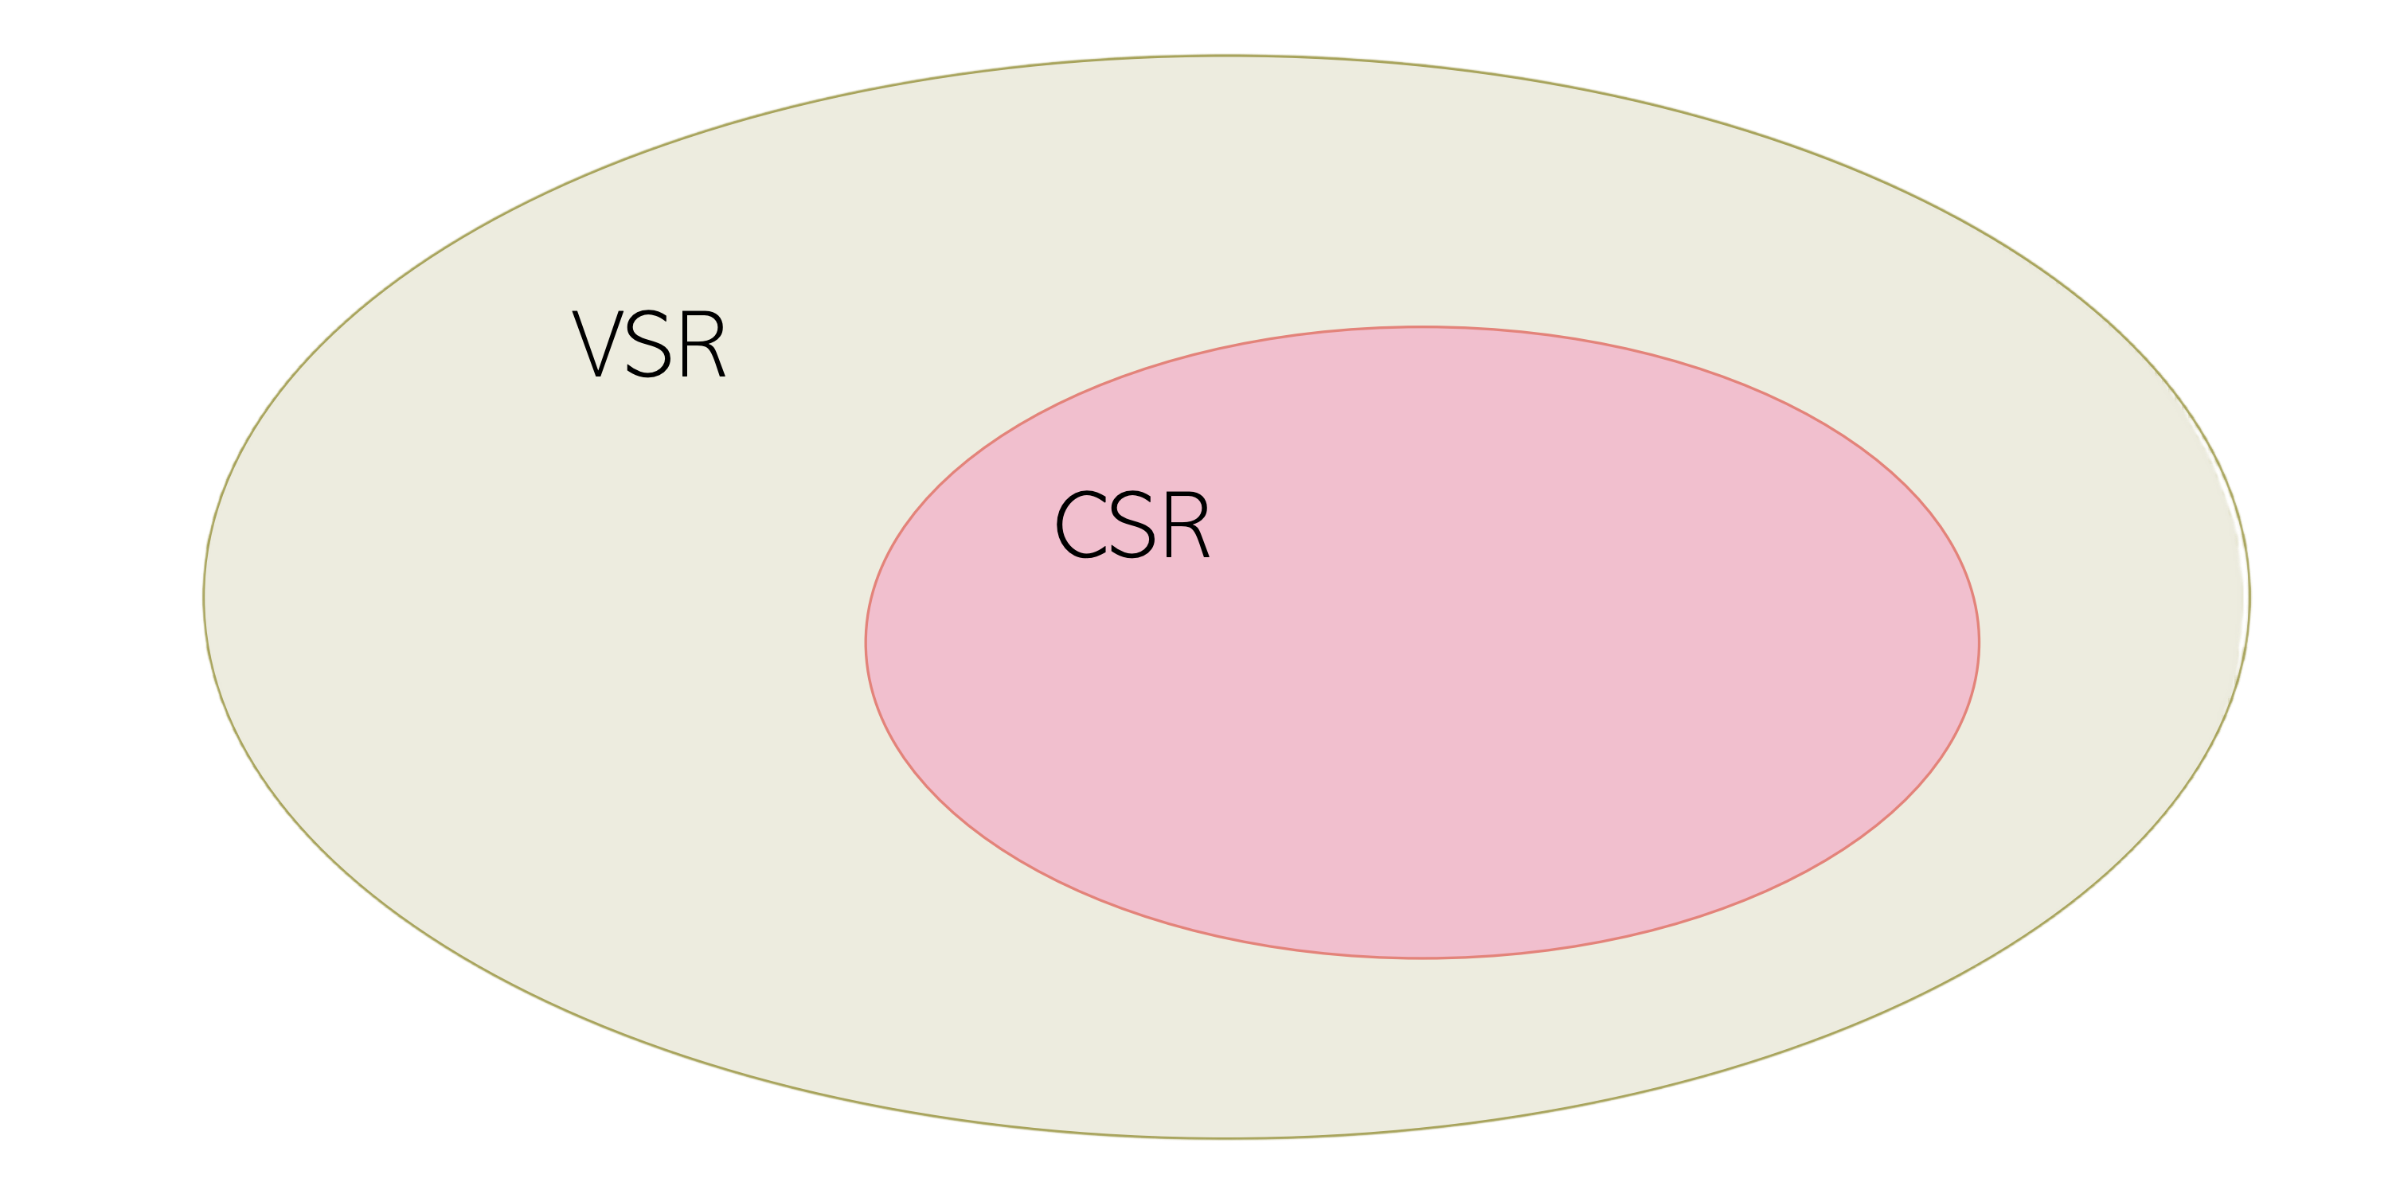
\includegraphics[width=0.5\textwidth]{images/VSR-CSR.png}
     \caption{relazione tra conflict-serializzabilità e view-serializzabilità}   
    \end{figure}

    \textbf{Dimostrazione}

    S è CSR $\Rightarrow$ S è VSR (se S non è CSR, allora non si può dire nulla sulla VSR).

    \begin{itemize}[label=$\triangleright$, itemsep=\medskipamount]
        \item \textbf{dimostrazione che} $\mathbf{CSR \subset VSR}$: basta trovare un controesempio
        \[
            \mathbf{S \in VSR} \text{ ma } \mathbf{S \notin CSR}
        \]

        Consideriamo:
        \[
           \mathrm{ S = r_1(x); w_2(x); w_1(x); w_3(x)}
        \]

        Gli insiemi sono:
        \begin{itemize}[label=$\diamond$, itemsep=\smallskipamount]
            \item \texttt{LEGGE\_DA(S)} = $\emptyset$
            \item \texttt{SCRITTURE\_FINALI(S)} = $\{\mathrm{w_3(x)}\}$
        \end{itemize}

        \smallskip
        Quindi questo schdeule è VSR perchè esiste uno schdeule $\mathrm{S_r}$ tale che $\mathrm{S_r \ \approx_V S}$:
        \[
            \mathrm{S_r = r_1(x); w_2(x); w_1(x); w_3(x)}
        \]

        che ha gli stessi insiemi:
        \begin{itemize}[label=$\diamond$, itemsep=\smallskipamount]
            \item \texttt{LEGGE\_DA($\mathrm{S_r}$)} = $\emptyset$
            \item \texttt{SCRITTURE\_FINALI($\mathrm{S_r}$)} = $\{\mathrm{w_3(x)}\}$
        \end{itemize}

        \smallskip
        Ora dimostriamo che questo schdeule non è CSR.

        Il suo insieme dei conflitti è:
        \[
            \begin{aligned}
                \texttt{CONFLITTI(S)} &= \{(\mathrm{r_1(x), w_2(x)), (r_1(x), w_3(x)), (w_2(x), w_1(x)), (w_2(x), w_3(x)})\}\\
                &= \{(\mathrm{w_1(x), w_3(x)})\}
            \end{aligned}
        \]

        Costruiamo il grafico dei conflitti:
        \begin{figure}[H]
            \centering
            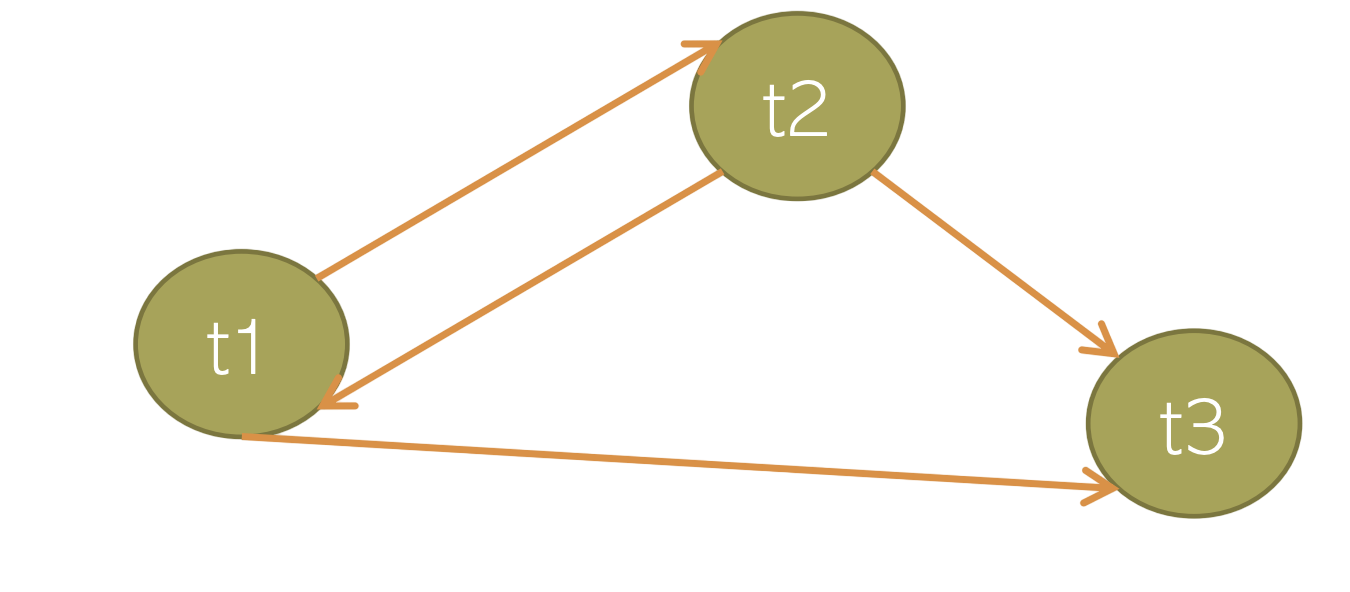
\includegraphics[width=0.45\textwidth]{images/grafico-conflitti.png}
        \end{figure}

        \item \textbf{dimostrazione che} $\mathbf{CSR \Rightarrow VSR}$: ($S_1 \approx_C S_2$ e $s_1 \approx_V S_2$)
        \begin{itemize}[label=$\circ$, itemsep=\medskipamount]
            \item $\mathrm{S_1}$ e $\mathrm{S_2}$ devono avere lo stesso insieme di \texttt{SCRITTURE\_FINALI}, altrimenti ci sarebbero due scritture sulla stessa risorsa da parte di transazioni in un ordine diverso e questo produrebbe un conflitto diverso
            \item devono avere lo stesso insieme di \texttt{LEGGE\_DA}, altrimenti ci sarebbe un conflitto, composto da una lattera e una scrittura, diverso e, quindi, siccome il conflitto è diverso, allora $\mathrm{S_1}$ e $\mathrm{S_2}$ non sono conflit-equivalenti
        \end{itemize}
    \end{itemize}

    \medskip
    Quindi se $\mathrm{S}$:
    \begin{itemize}[label=$\triangleright$, itemsep=\smallskipamount]
        \item \textbf{è CSR} $\Rightarrow$ $\mathbf{S}$ \textbf{è VSR}
        \item \textbf{non è CSR} $\Rightarrow$ $\mathbf{S}$ \textbf{non è VSR}
    \end{itemize}
}

\esempio{}{
  Consideriamo il seguente schedule:
  \[
    \mathrm{S_1 = r_1(x); \; w_1(x); \; r_2(z); \; r_1(y); \; w_1(y); \; r_2(x); \; w_2(x); \;
    w_2(z);}
  \]

  Verifichiamo se \( \mathrm{S_1} \) è VSR e per farlo vediamo se prima è CSR controllando
  l'insieme dei conflitti:
  \[
    \texttt{CONFLITTI}(\mathrm{S_1}) = \left\{ (\mathrm{r_1(x), w_2(x)),\; (w_1(x), r_2(x)),\; (w_1(x), w_2(x)}) \right\}
  \] 
  Costruiamo il grafo dei conflitti:
  \begin{figure}[H]
    \centering
    \begin{tikzpicture}[
      node distance=2cm
      ]
      \node[circle, draw] (t1) at (0,0) {\( t_1 \)};
      \node[circle, draw, right of=t1] (t2) {\( t_2 \)};

      \draw[->] (t1) to node[above] {} (t2);
    \end{tikzpicture}
  \end{figure}

  \smallskip
  Siccome il grafo è aciclico, allora \( \mathrm{S_1} \) è CSR e, quindi, \( \mathrm{S_1} \) è VSR.
}

\esempio{}{
  Consideriamo lo schedule:
  \[
    \mathrm{S_2 = r_1(x); \; w_1(x); \; w_3(x); \; r_2(y); \; r_3(y); \; w_3(y); \; w_1(y); \;
    r_2(x);}
  \] 

  Verifichiamo se \( \mathrm{S_2} \) è VSR e per farlo vediamo se prima è CSR controllando
  l'insieme dei conflitti:
  \[
    \begin{aligned}
      \texttt{CONFLITTI}(\mathrm{S_2}) =& 
      \{
        (\mathrm{r_1(x), w_3(x)}),\;
        (\mathrm{w_1(x), w_3(x)}),\;
        (\mathrm{w_1(x), r_2(x)}), \\
                             &(\mathrm{w_3(x), r_2(x)}),\;
                             (\mathrm{r_2(y), w_3(y)}),\;
                             (\mathrm{r_2(y), w_1(y)}), \\
                             &(\mathrm{r_3(y), w_1(y)}),\;
                             (\mathrm{w_3(y), w_1(y)})
                           \} 
    \end{aligned}
  \]

  Costruiamo il grafo dei conflitti:
  \begin{figure}[H]
    \centering
    \begin{tikzpicture}
      \node[circle, draw] (t1) at (0,0) {\( t_1 \)};
      \node[circle, draw] (t2) at (1.5,1.5) {\( t_2 \)};
      \node[circle, draw] (t3) at (3,0) {\( t_3 \)};

      \draw[->] (t1) edge [bend left=20] node[above] {} (t2);
      \draw[->] (t2) edge [bend left=20] node[above] {} (t1);
      \draw[->] (t1) edge [bend left=20] node[above] {} (t3);
      \draw[->] (t3) edge [bend left=20] node[above] {} (t1);
      \draw[->] (t3) edge [bend left=20] node[above] {} (t2);
      \draw[->] (t2) edge [bend left=20] node[above] {} (t3);
    \end{tikzpicture}
  \end{figure}
  \noindent
  Il grafo è ciclico, quindi \( \mathrm{S_2} \) \textbf{non è conflict-serializzabile} e di
  conseguenza \( \mathrm{S_2} \) \textbf{non è view-serializzabile}.
}

\esempio{}{
    Consideriamo lo schedule:
  \[
    \begin{aligned}
      \mathrm{S_3} =& \mathrm{r_1(x)}; \; \mathrm{r_2(x)}; \; \mathrm{w_2(x)}; \; \mathrm{r_3(x)}; \; \mathrm{r_4(z)}; \; \mathrm{w_1(x)}; \; \mathrm{w_3(y)}; \;
      \mathrm{w_3(x)}; \; \mathrm{w_1(y)};\\
           &\mathrm{w_5(x)}; \; \mathrm{w_1(z)}; \; \mathrm{w_5(y)}; \; \mathrm{r_5(z)};
    \end{aligned}
  \] 
  Verifichiamo se \( \mathrm{S_3} \) è VSR, per farlo vediamo se prima è CSR controllando
  l'insieme dei conflitti:
  \[
    \begin{aligned}
      \texttt{CONFLITTI}(\mathrm{S_3}) =& \{
        (\mathrm{r_1(x), w_2(x)}),\;
        (\mathrm{r_1(x), w_3(x)}),\;
        (\mathrm{r_1(x), w_5(x)}), \\
                      &(\mathrm{r_2(x), w_1(x)}),\;
        (\mathrm{r_2(x), w_3(x)}),\;
        (\mathrm{r_2(x), w_5(x)}), \\
                      &(\mathrm{w_2(x), r_3(x)}),\;
        (\mathrm{w_2(x), w_1(x)}),\;
        (\mathrm{w_2(x), w_3(x)}), \\
                      &(\mathrm{w_2(x), w_5(x)}),\;
        (\mathrm{r_3(x), w_1(x)}),\;
        (\mathrm{r_3(x), w_5(x)}), \\
                      &(\mathrm{r_4(z), w_1(z)}),\;
        (\mathrm{w_1(x), w_3(x)}),\;
        (\mathrm{w_1(x), w_5(x)}), \\
                      &(\mathrm{w_3(y), w_1(y)}),\;
        (\mathrm{w_3(y), w_5(y)}),\;
        (\mathrm{w_3(x), w_5(x)}), \\
                      &(\mathrm{w_1(y), w_5(y)}),\;
        (\mathrm{w_1(z), r_5(z)})
      \} 
    \end{aligned}
  \] 
  Il grafo dei conflitti è ciclico, allora \( \mathrm{S_3} \) \textbf{non è conflict-serializzabile} e di conseguenza \( \mathrm{S_3} \) \textbf{non è view-serializzabile}.
}

\subsection{Locking a due fasi stretto}
Il \textbf{locking a due fasi} (2PL) è il metodo applicato nei sistemi reali per la gestione dell'esecuzione concorrente delle transazioni perchè non richiede di conoscere in anticipo l'esito delle transazioni.\\[0.2ex]
\hl{Il locking a due fasi è un sottoinsieme della conflict-serializzabilità}.

\smallskip
Gli aspetti che caratterizzano il locking a due fasi sono i seguenti:
\begin{itemize}[label=$\triangleright$, itemsep=\medskipamount]
  \item \textbf{meccanismo di base per la gestione dei lock}: si basa sull'introduzione di alcune primitive di lock che consentono alle transazioni di bloccare le risorse sulle quali vogliono agire con operazioni di lettura e scrittura. 
  
  Le primitive di lock sono le seguenti:
  \begin{itemize}[label=$\diamond$, itemsep=\smallskipamount]
    \item \( \mathbf{r\_lock_K(x)} \): richiesta di un lock \textbf{condiviso} da parte della
      transazione \( \mathrm{t_K} \) sulla risorsa \( \mathrm{x} \) per eseguire una lettura

    \item \( \mathbf{w\_lock_K(x)} \): richiesta di un lock \textbf{esclusivo} da parte della
      transazione \( \mathrm{t_K} \) sulla risorsa \( \mathrm{x} \) per eseguire una scrittura

    \item \(\mathbf{ unlock_K(x)} \): richiesta da parte della transazione \( \mathrm{t_K} \) di liberare la risorsa \( \mathrm{x} \) da un precedente lock
  \end{itemize}
  
  \smallskip
  Le transazioni devono seguire le seguenti regole per applicare le primitive di
  lock:
  \begin{itemize}[label=$\circ$, itemsep=\smallskipamount]
    \item ogni \textbf{lettura} deve essere preceduta da un \( \mathrm{r\_lock} \) e seguita
      da un \( \mathrm{unlock} \). 
      
      Sono ammessi più \( \mathrm{r\_lock} \) contemporanei sulla stessa risorsa (lock condiviso)

    \item ogni \textbf{scrittura} deve essere preceduta da un \( \mathrm{w\_lock} \) e seguita da un \( \mathrm{unlock} \). 
    
    Non sono ammessi più \( \mathrm{w\_lock} \) (oppure \( \mathrm{w\_lock} \) e \( \mathrm{r\_lock} \)) contemporanei sulla stessa risorsa (lock esclusivo)
  \end{itemize}
  
  Se una transazione segue le precedenti regole, allora si dice \textbf{ben formata} rispetto al locking.

  \item \textbf{politica di concessione dei lock sulle risorse}: il gestore dei lock (o gestore della concorrenza) mantiene per ogni risorsa \( \mathrm{x} \) le seguenti informazioni:
  \begin{itemize}[label=$\diamond$, itemsep=\smallskipamount]
    \item \textbf{stato}: \( \mathrm{s(x)} \in \left\{ \mathrm{libero}, \mathrm{r\_lock}, \mathrm{w\_lock} \right\} \) 

    \item \textbf{transazioni in r\_lock}: \( \mathrm{c(x)} = \left( \mathrm{t_1, \dots, t_n} \right)  \), dove \( \mathrm{t_1, \ldots, t_n} \) hanno un \( \mathrm{r\_lock} \) su \( \mathrm{x} \)
  \end{itemize}
  Il comportamento del gestore dei lock è descritto dalla seguente tablella:
  \begin{figure}[H]
    \centering
    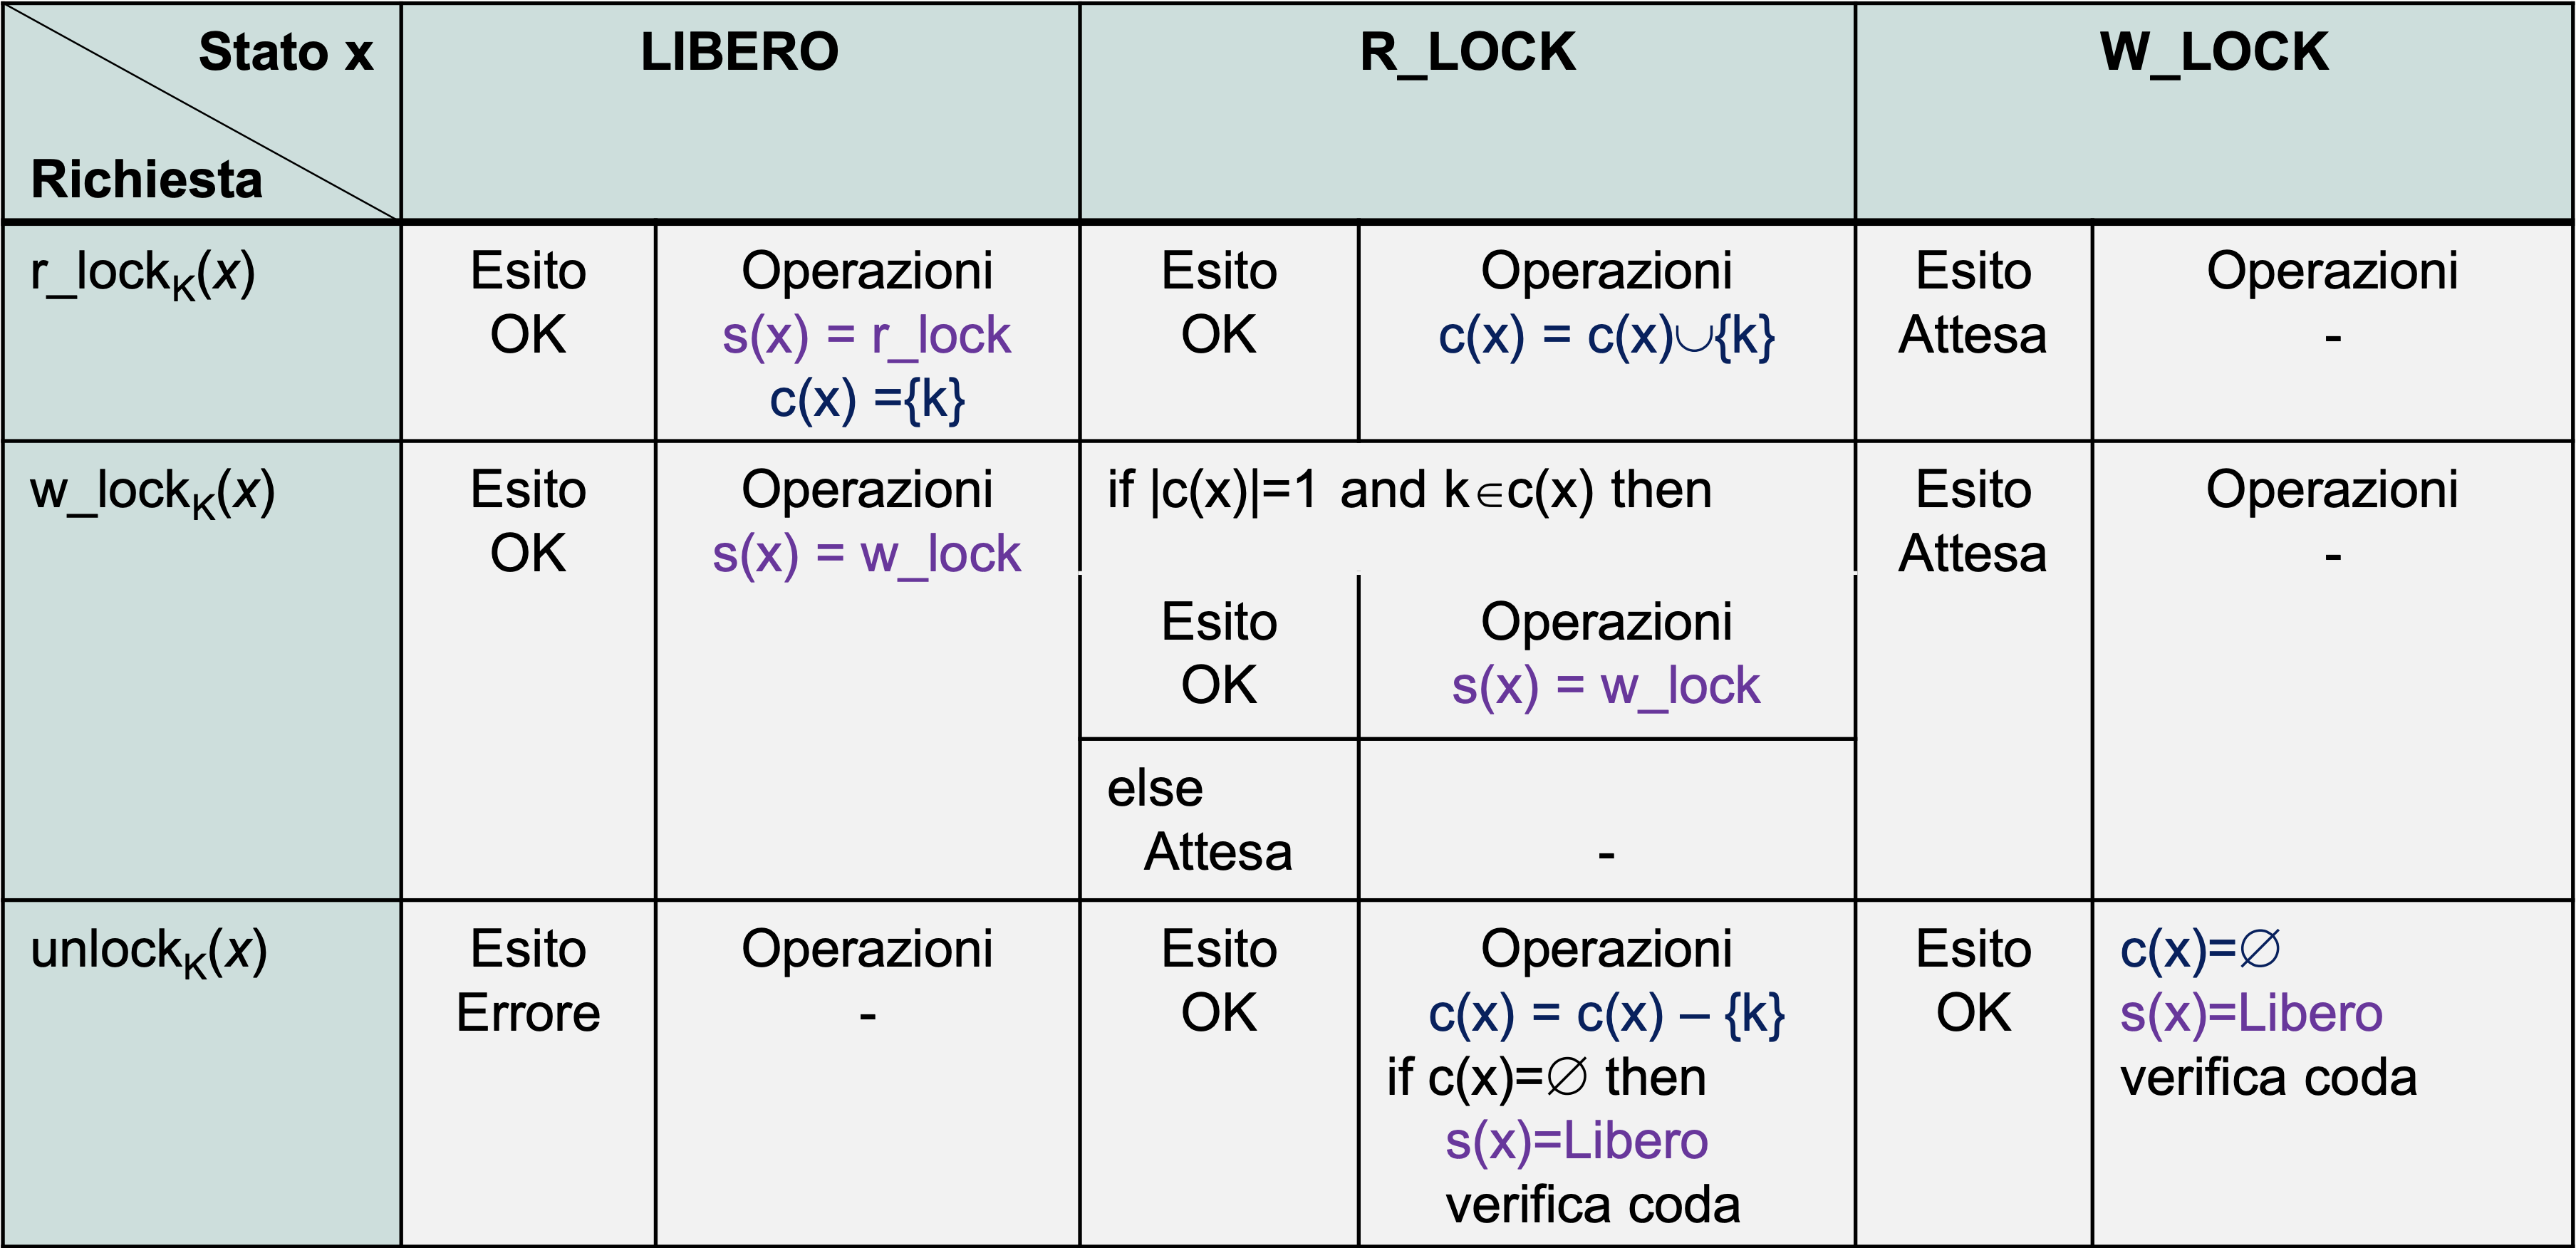
\includegraphics[width=0.5\textwidth]{images/gestore-lock.png}
  \end{figure}

  \item \textbf{regola che garantisce la serializzabilità}: una transazione dopo aver rilasciato un lock non può acquisirne altri.
  
  Questa regola è visualizzata dal seguente grafico:
  \begin{figure}[H]
    \centering
    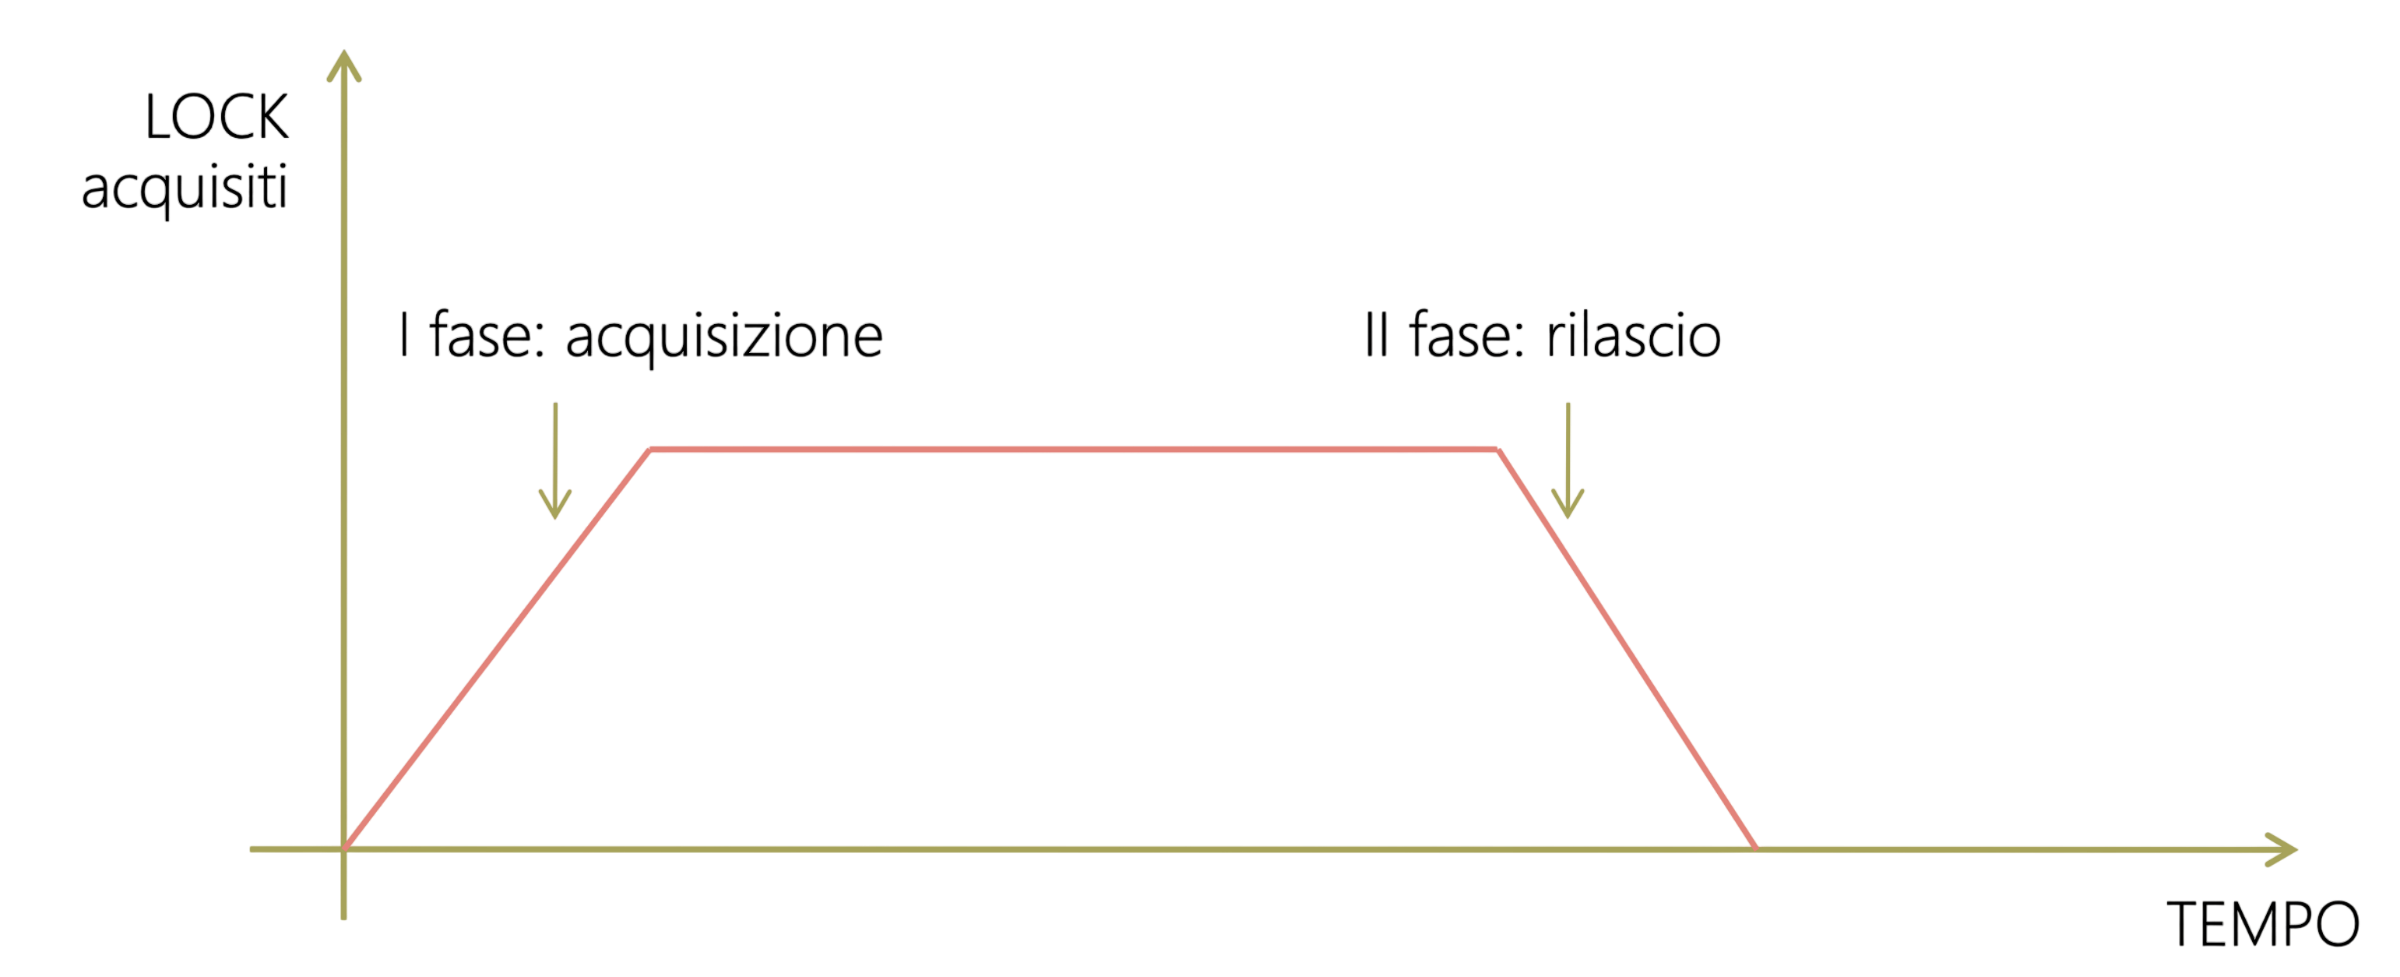
\includegraphics[width=0.6\textwidth]{images/locking-due-fasi.png}
    \caption{locking a due fasi}
  \end{figure}
\end{itemize}

\esempio{perdita di aggiornamento}{
    Consideriamo le seguenti transazioni:
  \[
  \begin{aligned}
    \mathrm{t_1}:\; & \mathrm{r_1(x)}; \; \mathrm{w_1(x)} \\
    \mathrm{t_2}:\; & \mathrm{r_2(x)}; \; \mathrm{w_2(x)}
  \end{aligned}
  \]

  Eseguire lo schedule:
  \[
    \mathbf{S_{pa}:\; r_1(x); \; r_2(x); \; w_2(x); \; w_1(x);}
  \]

  \begin{enumerate}[itemsep=\smallskipamount]
    \item \( \mathrm{r_1(x)} \) richiede un \( \mathrm{r\_lock_1(x)} \) 
    \item \( \mathrm{r_2(x)} \) richiede un \( \mathrm{r\_lock_2(x)} \)
    \item \( \mathrm{w_2(x)} \) richiede un \( \mathrm{w\_lock_2(x)} \), ma lo stato \( \mathrm{s(x) = r\_lock} \), con \( \mathrm{c(x)} = \left\{ \mathrm{t_1, t_2} \right\} \), quindi, \( \mathrm{w_2(x)} \) per ottenere \( \mathrm{w\_lock_2(x)} \) deve attendere che \( \mathrm{t_1} \) rilasci \( \mathrm{r\_lock(x)} \) ma se \( \mathrm{t_1} \) rilascia \( \mathrm{r\_lock(x)} \) e, quindi, inizierebbe la sua fase discendente impedendogli di acquisire altri lock e di conseguenza \( \mathrm{w\_lock_1(x)} \) non è più possibile per la serializzabilità del 2PL
  \end{enumerate}

  \smallskip
  Di conseguenza questo schedule \textbf{non è 2PL}.
}

Il locking a due fasi stretto (strict 2PL) è una variante del locking a due fasi che introduce una condizione aggiuntiva per rimuovere la necessità dell'ipotesi di commit-proiezione. 

La condizione aggiuntiva è la seguente: Una transazione può rilasciare i lock solo quando ha eseguito correttamente un \texttt{commit} o un \texttt{rollback}.

\begin{figure}[H]
  \centering
  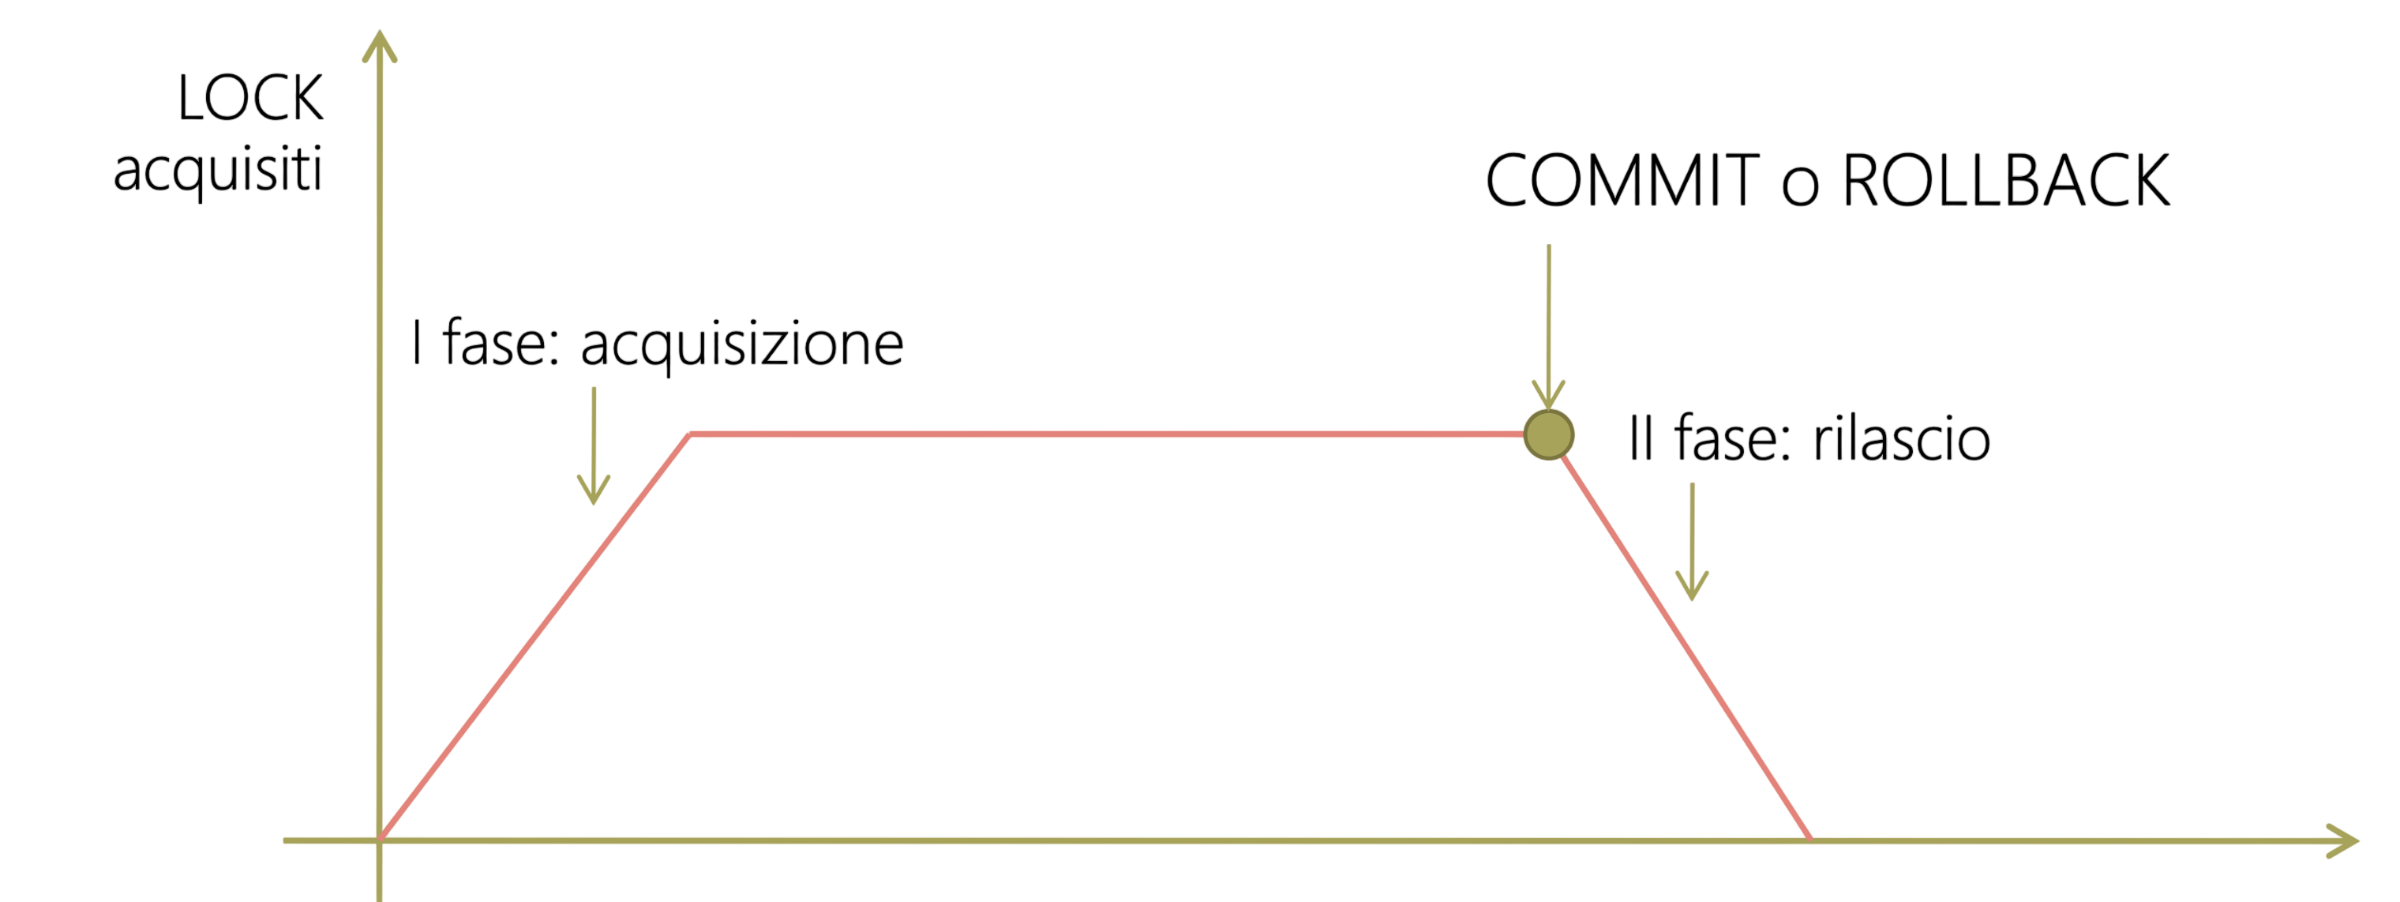
\includegraphics[width=0.6\textwidth]{images/locking-due-fasi-stretto.png}
  \caption{locking a due fasi stretto}
\end{figure}

\subsection{Blocco critico (deadlock)}
Il \textbf{blocco critico} è una situazione di blocco che si verifica nell'esecuzione di transazioni concorrenti quando:
\begin{itemize}[label=$\circ$, itemsep=\smallskipamount]
  \item due transazioni hanno bloccato delle risorse:
    \begin{itemize}
      \item \( \mathrm{t_1} \) ha bloccato \( \mathrm{r_1} \)

      \item \( \mathrm{t_2} \) ha bloccato \( \mathrm{r_2} \)
    \end{itemize}

  \item \( \mathrm{t_1} \) è in attesa sulla risorsa \( \mathrm{r_2} \) e \( \mathrm{t_2} \) è in attesa sulla risorsa \( \mathrm{r_1} \)
\end{itemize}

Se il numero medio di tuple per tabella è \( \mathrm{n} \) e la granularità del lock (numero di risorse che possono essere bloccate) è la tupla, la probabilità che si verifichi un lock tra due transazioni è:
\[
  \mathbf{P(\text{deadlock di lunghezza 2}) = \frac{1}{n^2}}
\]

\esempio{deadlock}{
  Un esempio di deadlock utilizzando il locking a due fasi stretto è il seguente:
  \begin{figure}[H]
    \centering
    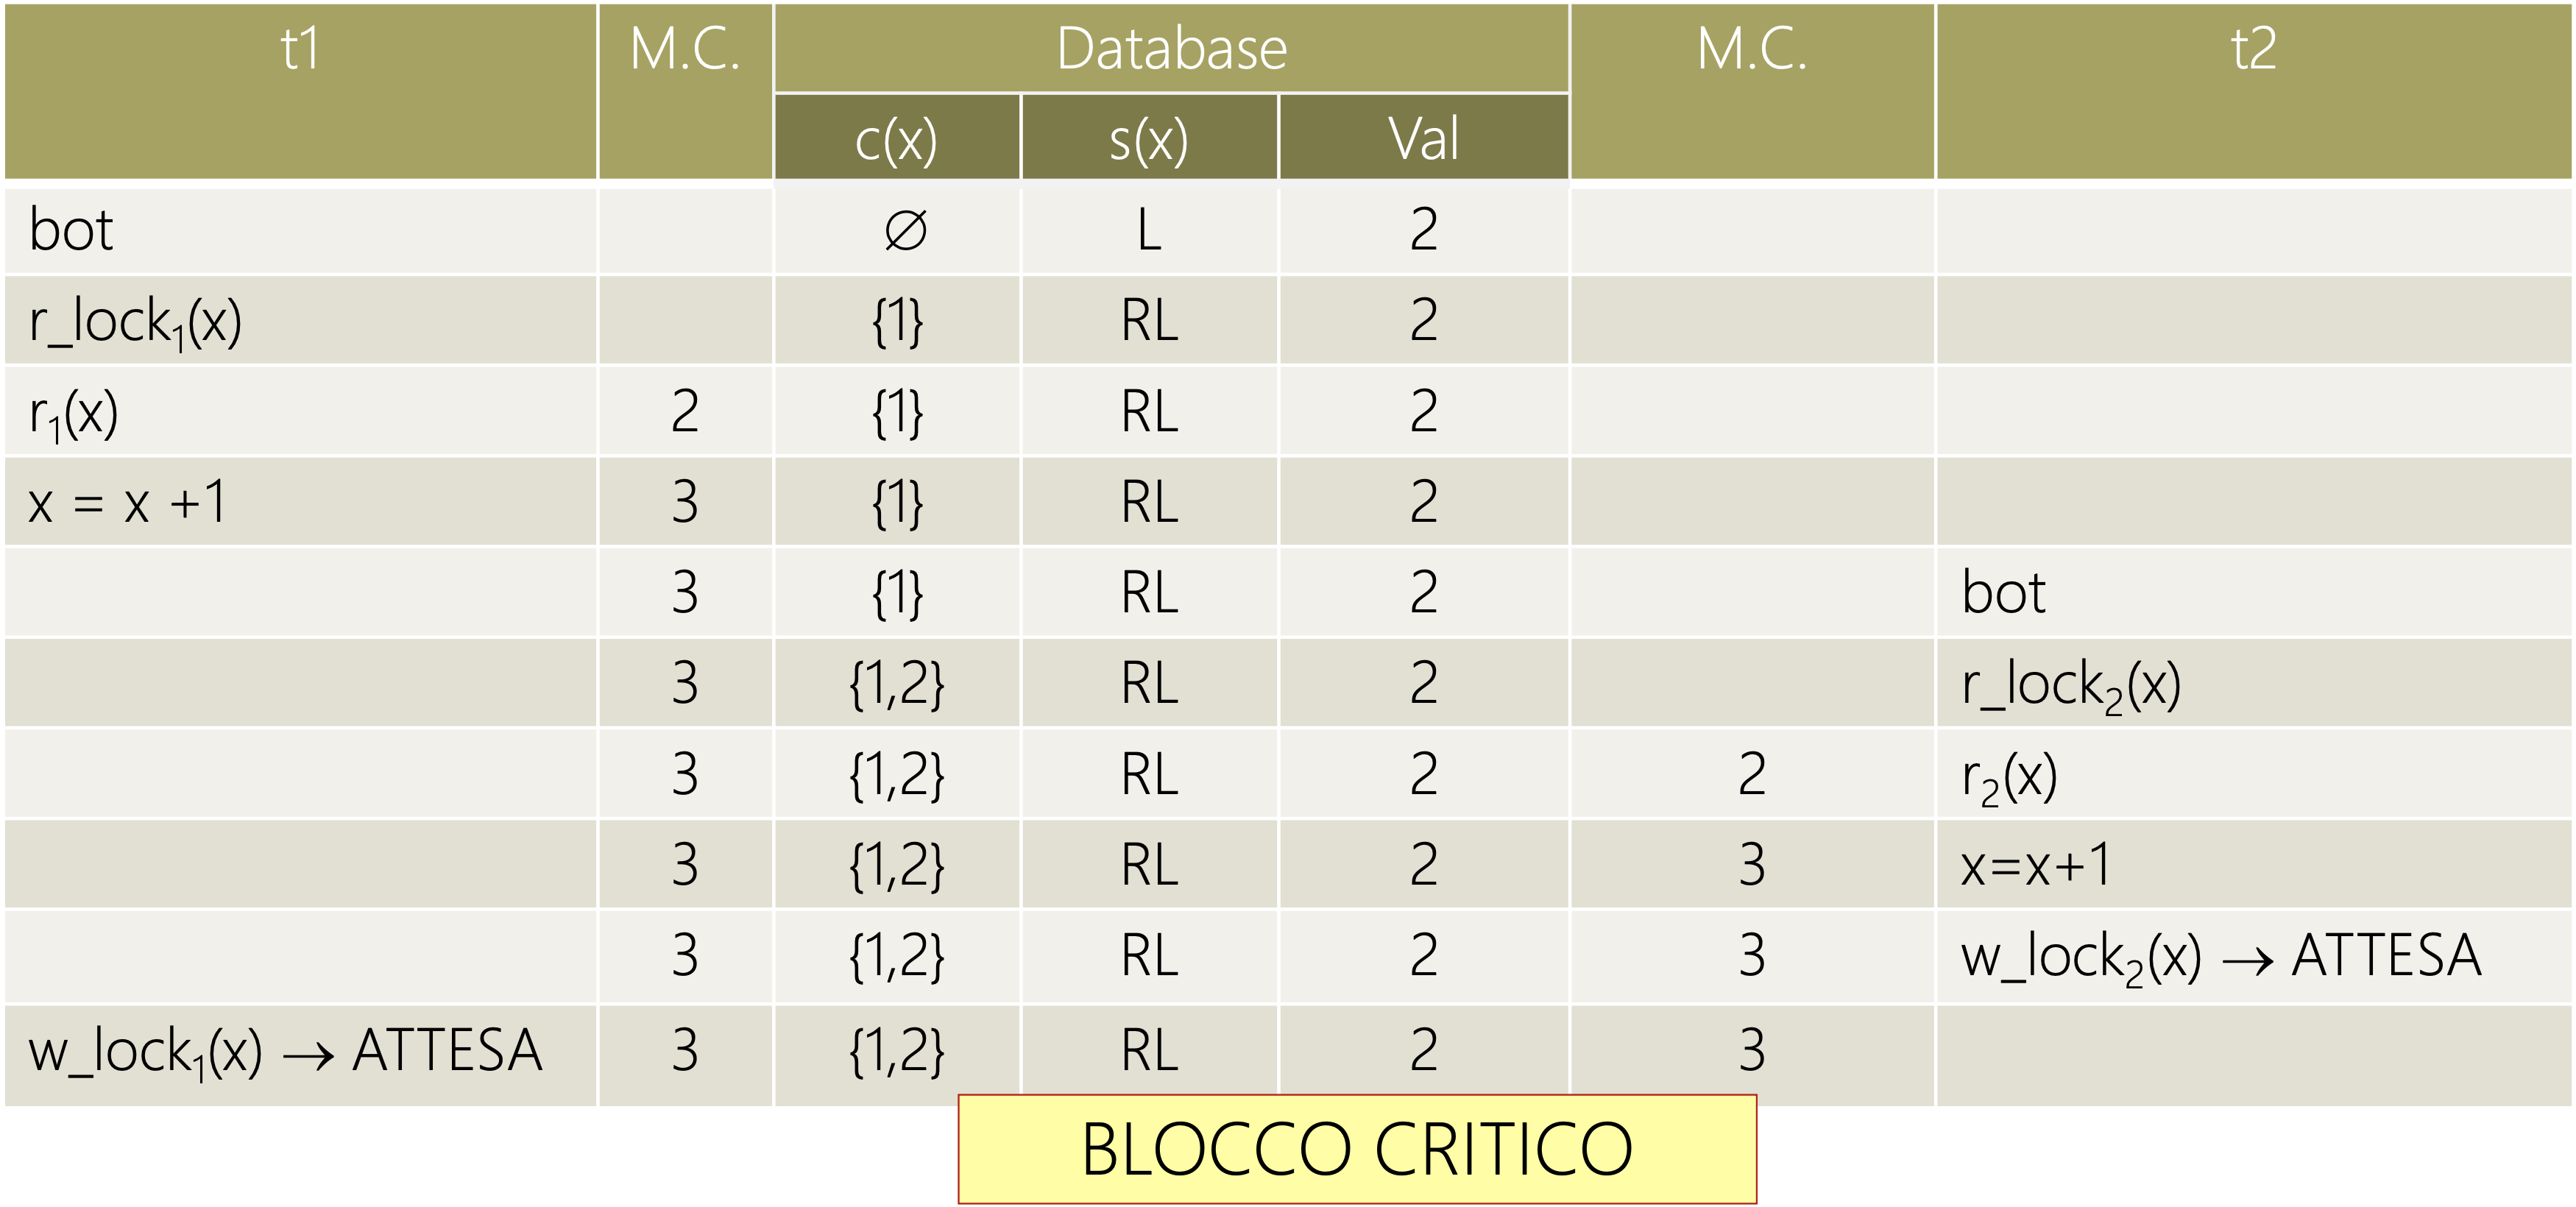
\includegraphics[width=0.7\textwidth]{images/deadlock-locking-due-fasi-stretto.png}
  \end{figure}
}

\noindent
Le tecniche per risolvere i deadlock sono le seguenti:
\begin{itemize}[label=$\diamond$, itemsep=\smallskipamount]
  \item \textbf{timeout}: se una transazione è in attesa su una risorsa da troppo tempo 
    viene abortita

  \item \textbf{prevenzione}: 
  \begin{itemize}[itemsep=\smallskipamount]
    \item una transazione blocca tutte le risorse a cui deve accedere in lettura o
      scrittura in una sola volta (o blocca tutto o non blocca nulla)

    \item ogni transazione \( \mathrm{t_i} \) acquisisce un timestamp \( \mathrm{TS_i} \) all'inizio della sua esecuzione. 
    
    La transazione \( \mathrm{t_i} \) può attendere una risorsa bloccata da \( \mathrm{t_j} \) solo se vale una certa condizione sui timestamp (es. \( \mathrm{TS_i < TS_j} \)), altrimenti \( \mathrm{t_i} \) viene abortita e fatta ripartire con lo stesso timestamp
  \end{itemize}

  \item \textbf{rilevamento}: si esegue un'analisi periodica della tabella di lock per rilevare la presenza di un deadlock che corrisponde ad un ciclo nel grafo delle relazioni di attesa.
  
  Questa tecnica è la più utilizzata nei sistemi reali.
\end{itemize}

Inoltre la scelta di gestire i lock in lettura come lock condivisi introduce il problema della \textbf{starvation} che tuttavia nel contesto delle DMBS risulta poco probabile, ma comunque risolvibile con le tecniche precedenti.

\definizione{starvation}{
  Se una risorsa \( \mathrm{x} \) viene costantemente bloccata da una sequenza di transazioni che acquisiscono \( \mathrm{r\_lock} \) su \( \mathrm{x} \), un'eventuale transazione in attesa di scrivere su \( \mathrm{x} \) viene bloccata per un lungo periodo fino alla fine della sequenza di letture.
  \begin{figure}[H]
    \centering
    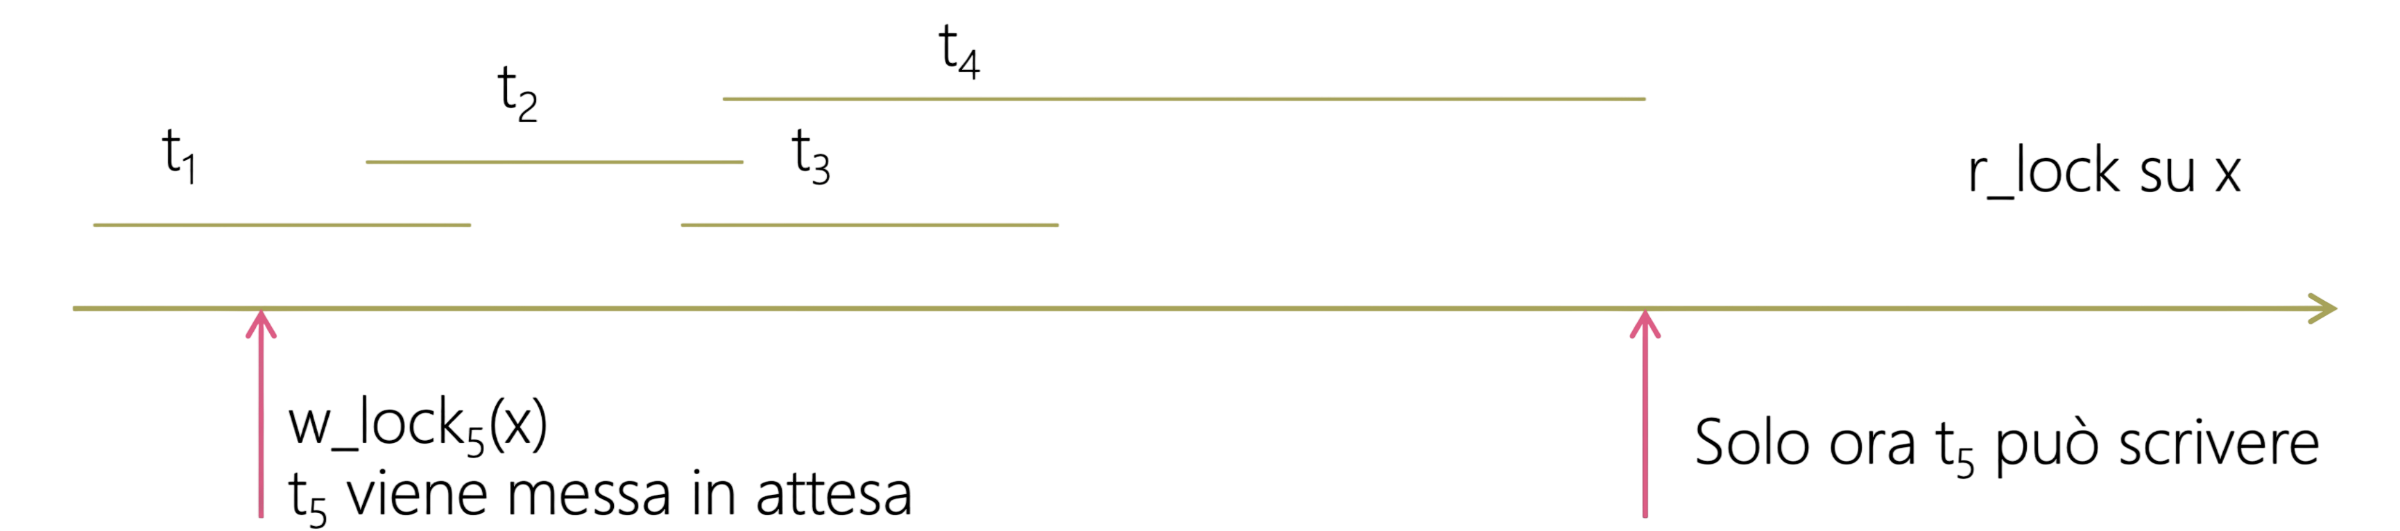
\includegraphics[width=0.7\textwidth]{images/starvation.png}
  \end{figure}
}

\subsection{Gestione della concorrenza in SQL}
Siccome risulta molto pesante per il sistema gestire l'esecuzione concorrente di
transazioni con una conseguente diminuzione delle prestazioni, SQL prevede la 
possibilità di \textbf{rinunciare del tutto o in parte al controllo di concorrenza}
per aumentare le prestazioni del sistema.\\[0.2ex]
È quindi possibile, a livello di una singola transazione, decidere di \textbf{tollerare alcune anomalie} di esecuzione concorrente.

\smallskip
La seguente tabella mostra le possibili combinazioni di anomalie che si possono tollerare:
\begin{figure}[H]
  \centering
  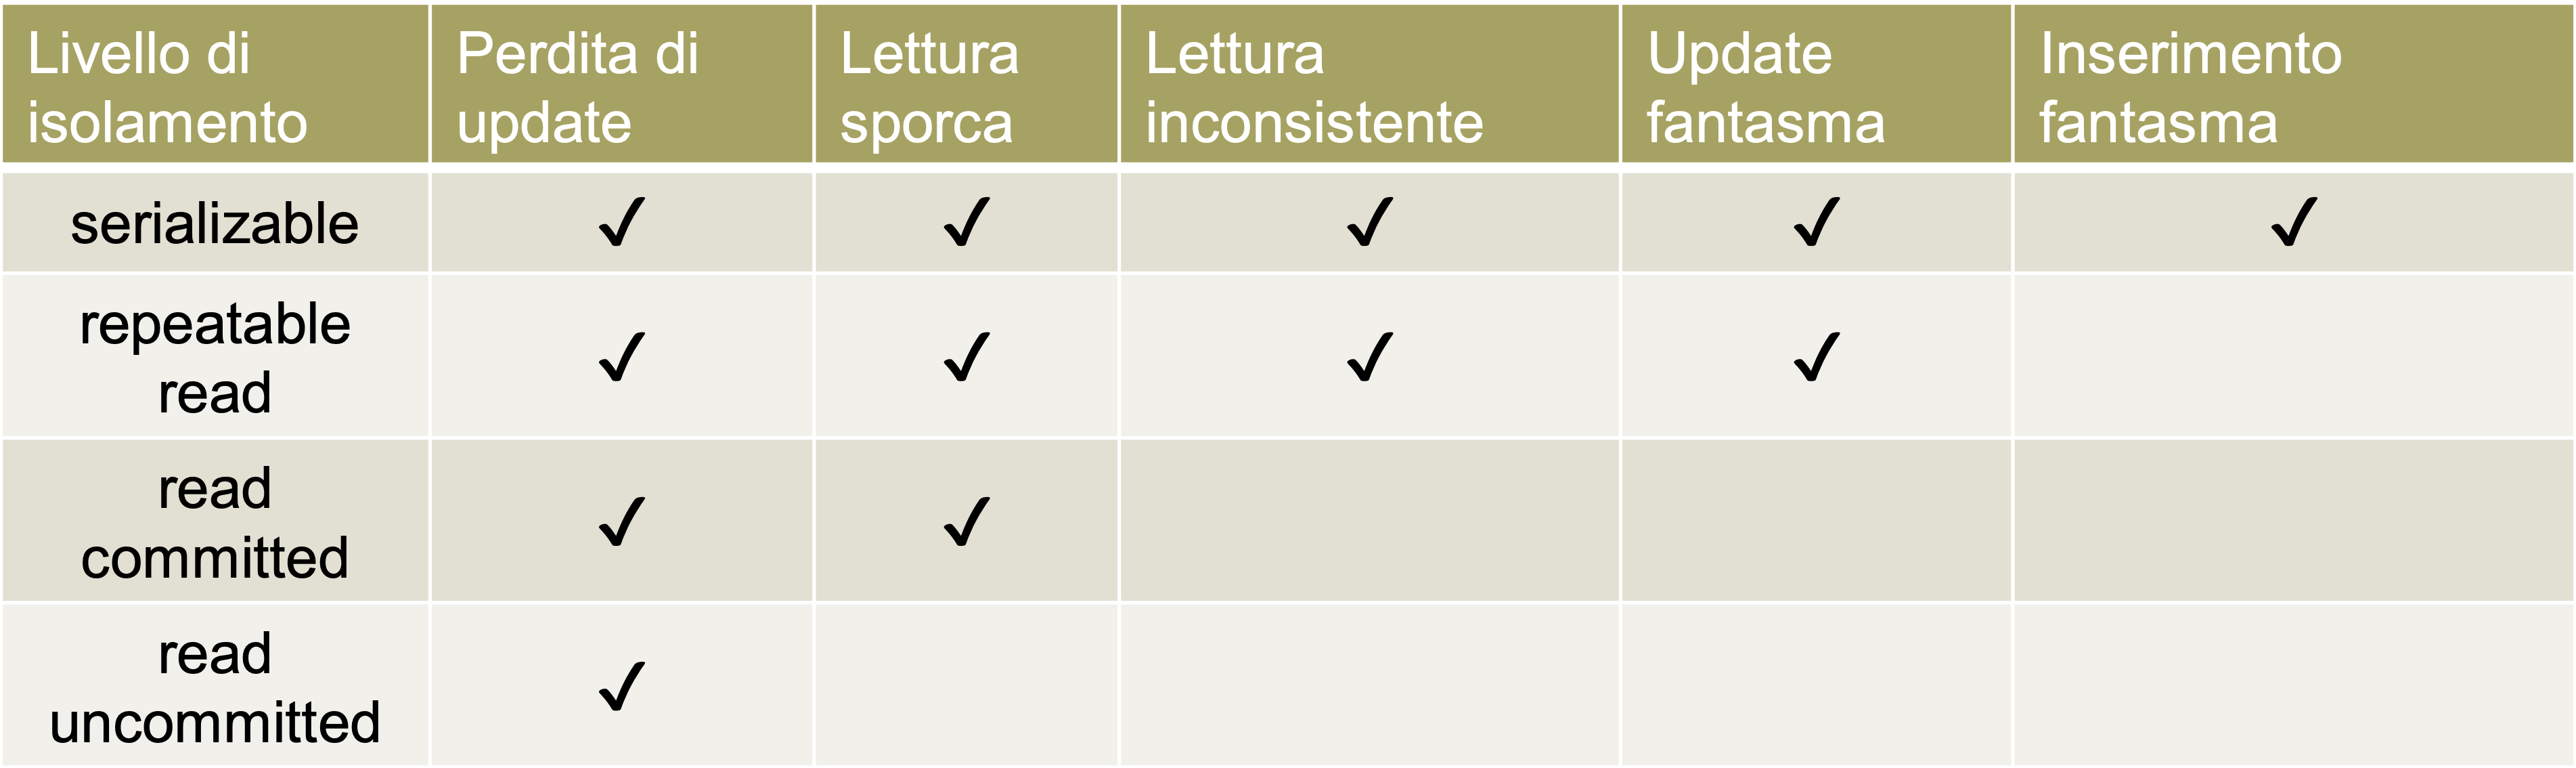
\includegraphics[width=0.7\textwidth]{images/anomalie-tollerate-SQL.png}
  \caption{Anomalie tollerate in SQL}
\end{figure}

\vario{Nota}{
    \begin{itemize}[label=$\triangleright$, itemsep=\smallskipamount]
        \item tutti i livelli richiedono il 2PL stretto per le scritture
        \item \textbf{serializable}: richiede il 2PL stretto anche per le letture e applica il lock sulle tabelle per evitare l'inserimento fantasma
        \item \textbf{repeatable read}: applica il 2PL stretto anche per le letture, ma applica i lock a livello di tupla e non di tabella.
        
        Consente inserimenti e, quindi, non evita l'anomalia di inserimento fantasma.

        \textcolor{red}{\textbf{Attenzione}}: in PostgreSQL la repeatable read è implementata in modo più stringente che evita anche l'anomalia di inserimento fantasma
        \item \textbf{read committed}: richiede lock condivisi per le letture, ma non il 2PL stretto
        \item \textbf{read uncommitted}: non applica lock in lettura
    \end{itemize}
}

    %!TeX root = BasiDiDati.tex

\chapter{Ottimizzazione di interrogazioni}
Ogni interrogazione sottomessa al DBMS viene espressa in un linguaggio dichiarativo (es. SQL).\\[0.2ex]
E' necessario, quindi, trovare un'equivalente espressione procedurale (es. algebra relazionale) per generare un piano di esecuzione.\\[0.2ex]
L'espressione algebrica va ottimizzata rispetto alle caratteristche del DBMS a livello fisico e dalla base di dati corrente.

\smallskip
Le fasi di ottimizzazione di una query conistono in:
\begin{enumerate}[itemsep=\smallskipamount]
    \item \textbf{analisi lessicale e sintattica}: verifica che la query sia scritta correttamente
    \item \textbf{ottimizzazione algebrica}: si basa sulle regole dell'algebra relazionale
    \begin{itemize}[label=$\circ$, itemsep=\smallskipamount]
        \item anticipo delle selezioni
        \item anticipo delle proiezioni
    \end{itemize}
    \item \textbf{ottimizzaione dipendente dai metodi di accesso}: si basa sulle statistiche e sulle strutture fisiche (profili delle tabelle)
    \item \textbf{generazione del codice}: si genera un piano di esecuzione per ottenere il risultato della query
\end{enumerate}

\begin{figure}[H]
    \centering
    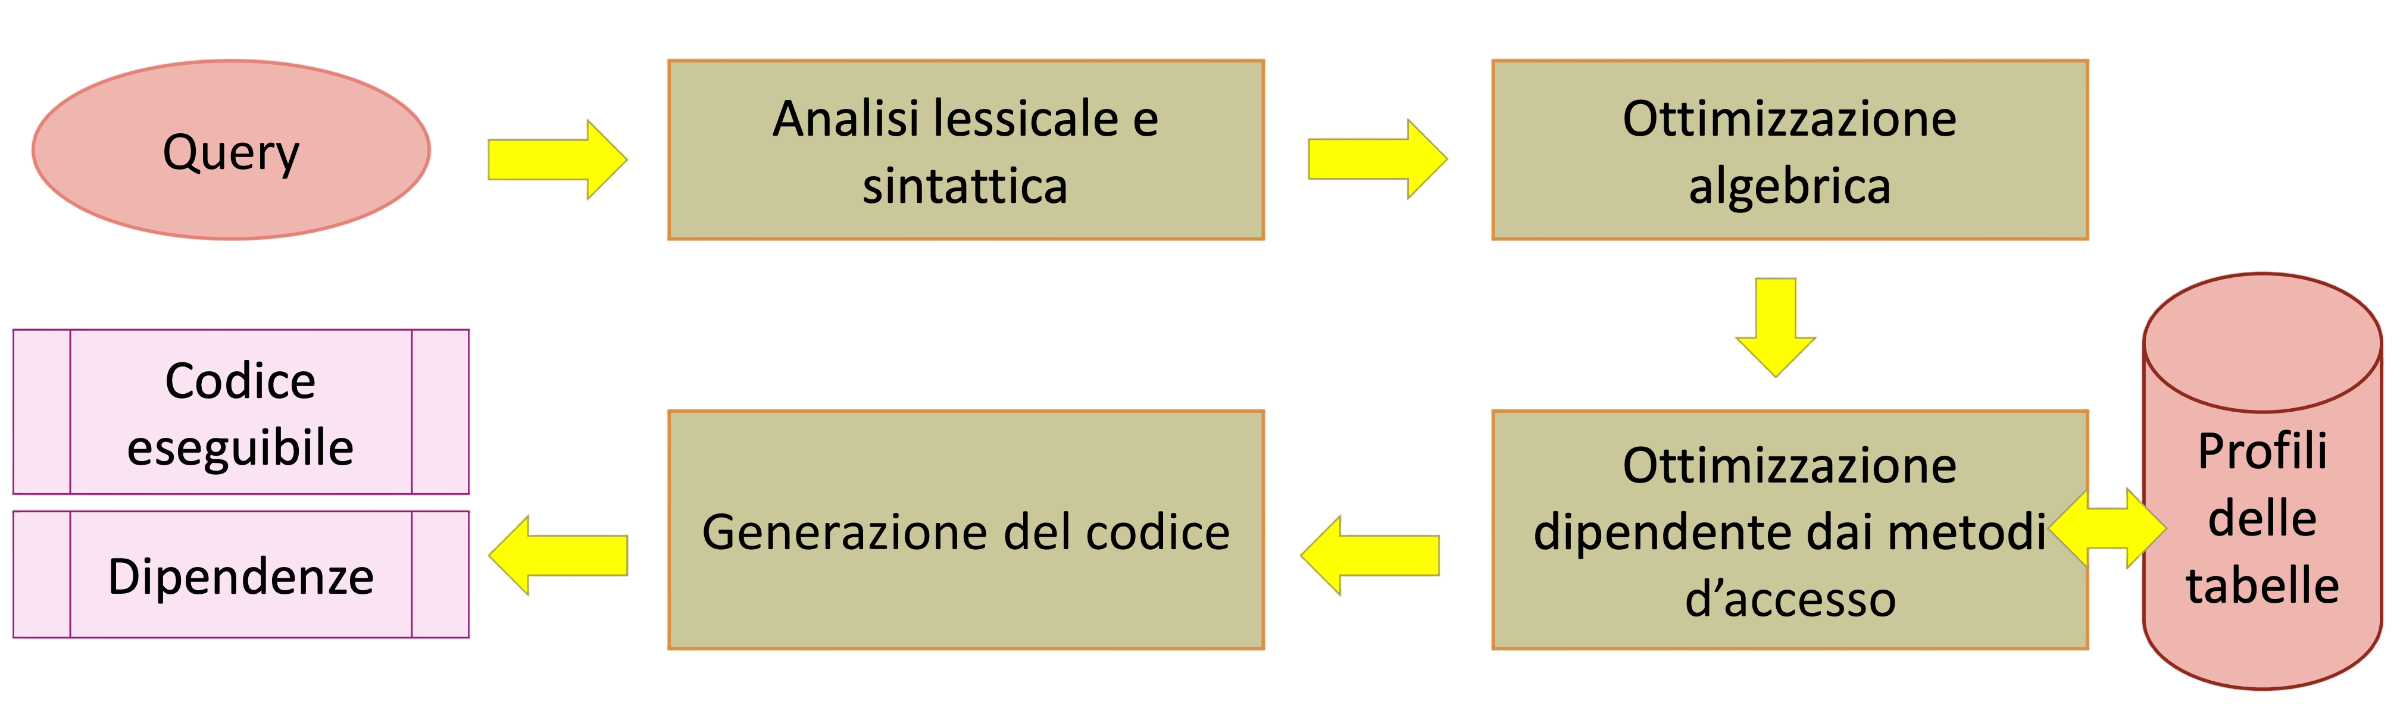
\includegraphics[width=0.75\textwidth]{images/ottimizzazione-query.png}
    \caption{processo di ottimizzazione di una query}
\end{figure}

\section{Ottimizzazione dipendente dai metodi di accesso}
Le operazioni tipiche di accesso supportate dal DBMS sono:
\begin{itemize}[label=$\triangleright$, itemsep=\smallskipamount]
    \item \textbf{scansione delle tuple di una tabella}
    \item \textbf{ordinamento delle tuple}
    \item \textbf{accesso diretto tramite indice}
    \item \textbf{join con diverse implementazioni}
\end{itemize}

\subsection{Scansione sequenziale}
L'operazione di scansione opera contestualmente altre operazioni:
\begin{itemize}[label=$\diamond$, itemsep=\smallskipamount]
    \item \textbf{scansione} + \textbf{proiezione} (senza eliminazione dei duplicati)
    \item \textbf{scansione} + \textbf{selezione} (rispetto a un predicato semplice)
    \item \textbf{scansione} + \textbf{inserimento/cancellazione/modifica}
\end{itemize}

\begin{itemize}[label=$\Rightarrow$, itemsep=\smallskipamount]
    \item \textcolor{red}{\textbf{costo scansione sequenziale}}: $\mathbf{NP(R)}$ (numero di pagine della relazione $\mathrm{R}$)
\end{itemize}

\subsection{Ordinamento}
L'ordinamento viene utilizzato per:
\begin{itemize}[label=$\diamond$, itemsep=\smallskipamount]
    \item \textbf{ordinare il risultato di un'interrogazione} (clausola \texttt{ORDER BY})
    \item \textbf{eliminare duplicati} (clausola \texttt{SELECT DISTINCT})
    \item \textbf{raggruppare tuple} (clausola \texttt{GROUP BY})
\end{itemize}

L'ordinamento viene eseguito su memoria secondaria utilizzando l'algoritmo \textbf{Z-way-Sort-Merge}:
\begin{enumerate}[itemsep=\smallskipamount]
    \item \textbf{sort interno}:
    \begin{enumerate}[itemsep=\smallskipamount]
        \item si leggono una alla volta le pagine della tabella
        \item le tuple di ogni pagina vengono ordinate con un algoritmo di sort interno (es. quick-sort)
        \item ogni pagina ordinata (run) viene scritta su memoria secondaria in un file temporaneo 
    \end{enumerate}
    \item \textbf{merge}: vengono unite le run in un'unica run
\end{enumerate}

\esempio{algoritmo Z-way-Sort-merge}{
    Supponiamo di dover ordinare un input che consiste in una tabella di $\mathrm{NP}$ pagine e di avere a disposizione sono $\mathrm{NB}$ buffer in memoria centrale ($\mathrm{NB < NP}$).

    Per semplicità, consideriamo il caso base a due vie ($\mathrm{Z} = 2$) e supponiamo di avere solo 3 buffer in memoria centrale ($\mathrm{NB} = 3$).

    \smallskip
    Si hanno 4 pagine composte da 3 tuple ciascuna e si vuole ordinare in base alla prima colonna:
    \begin{figure}[H]
        \centering
        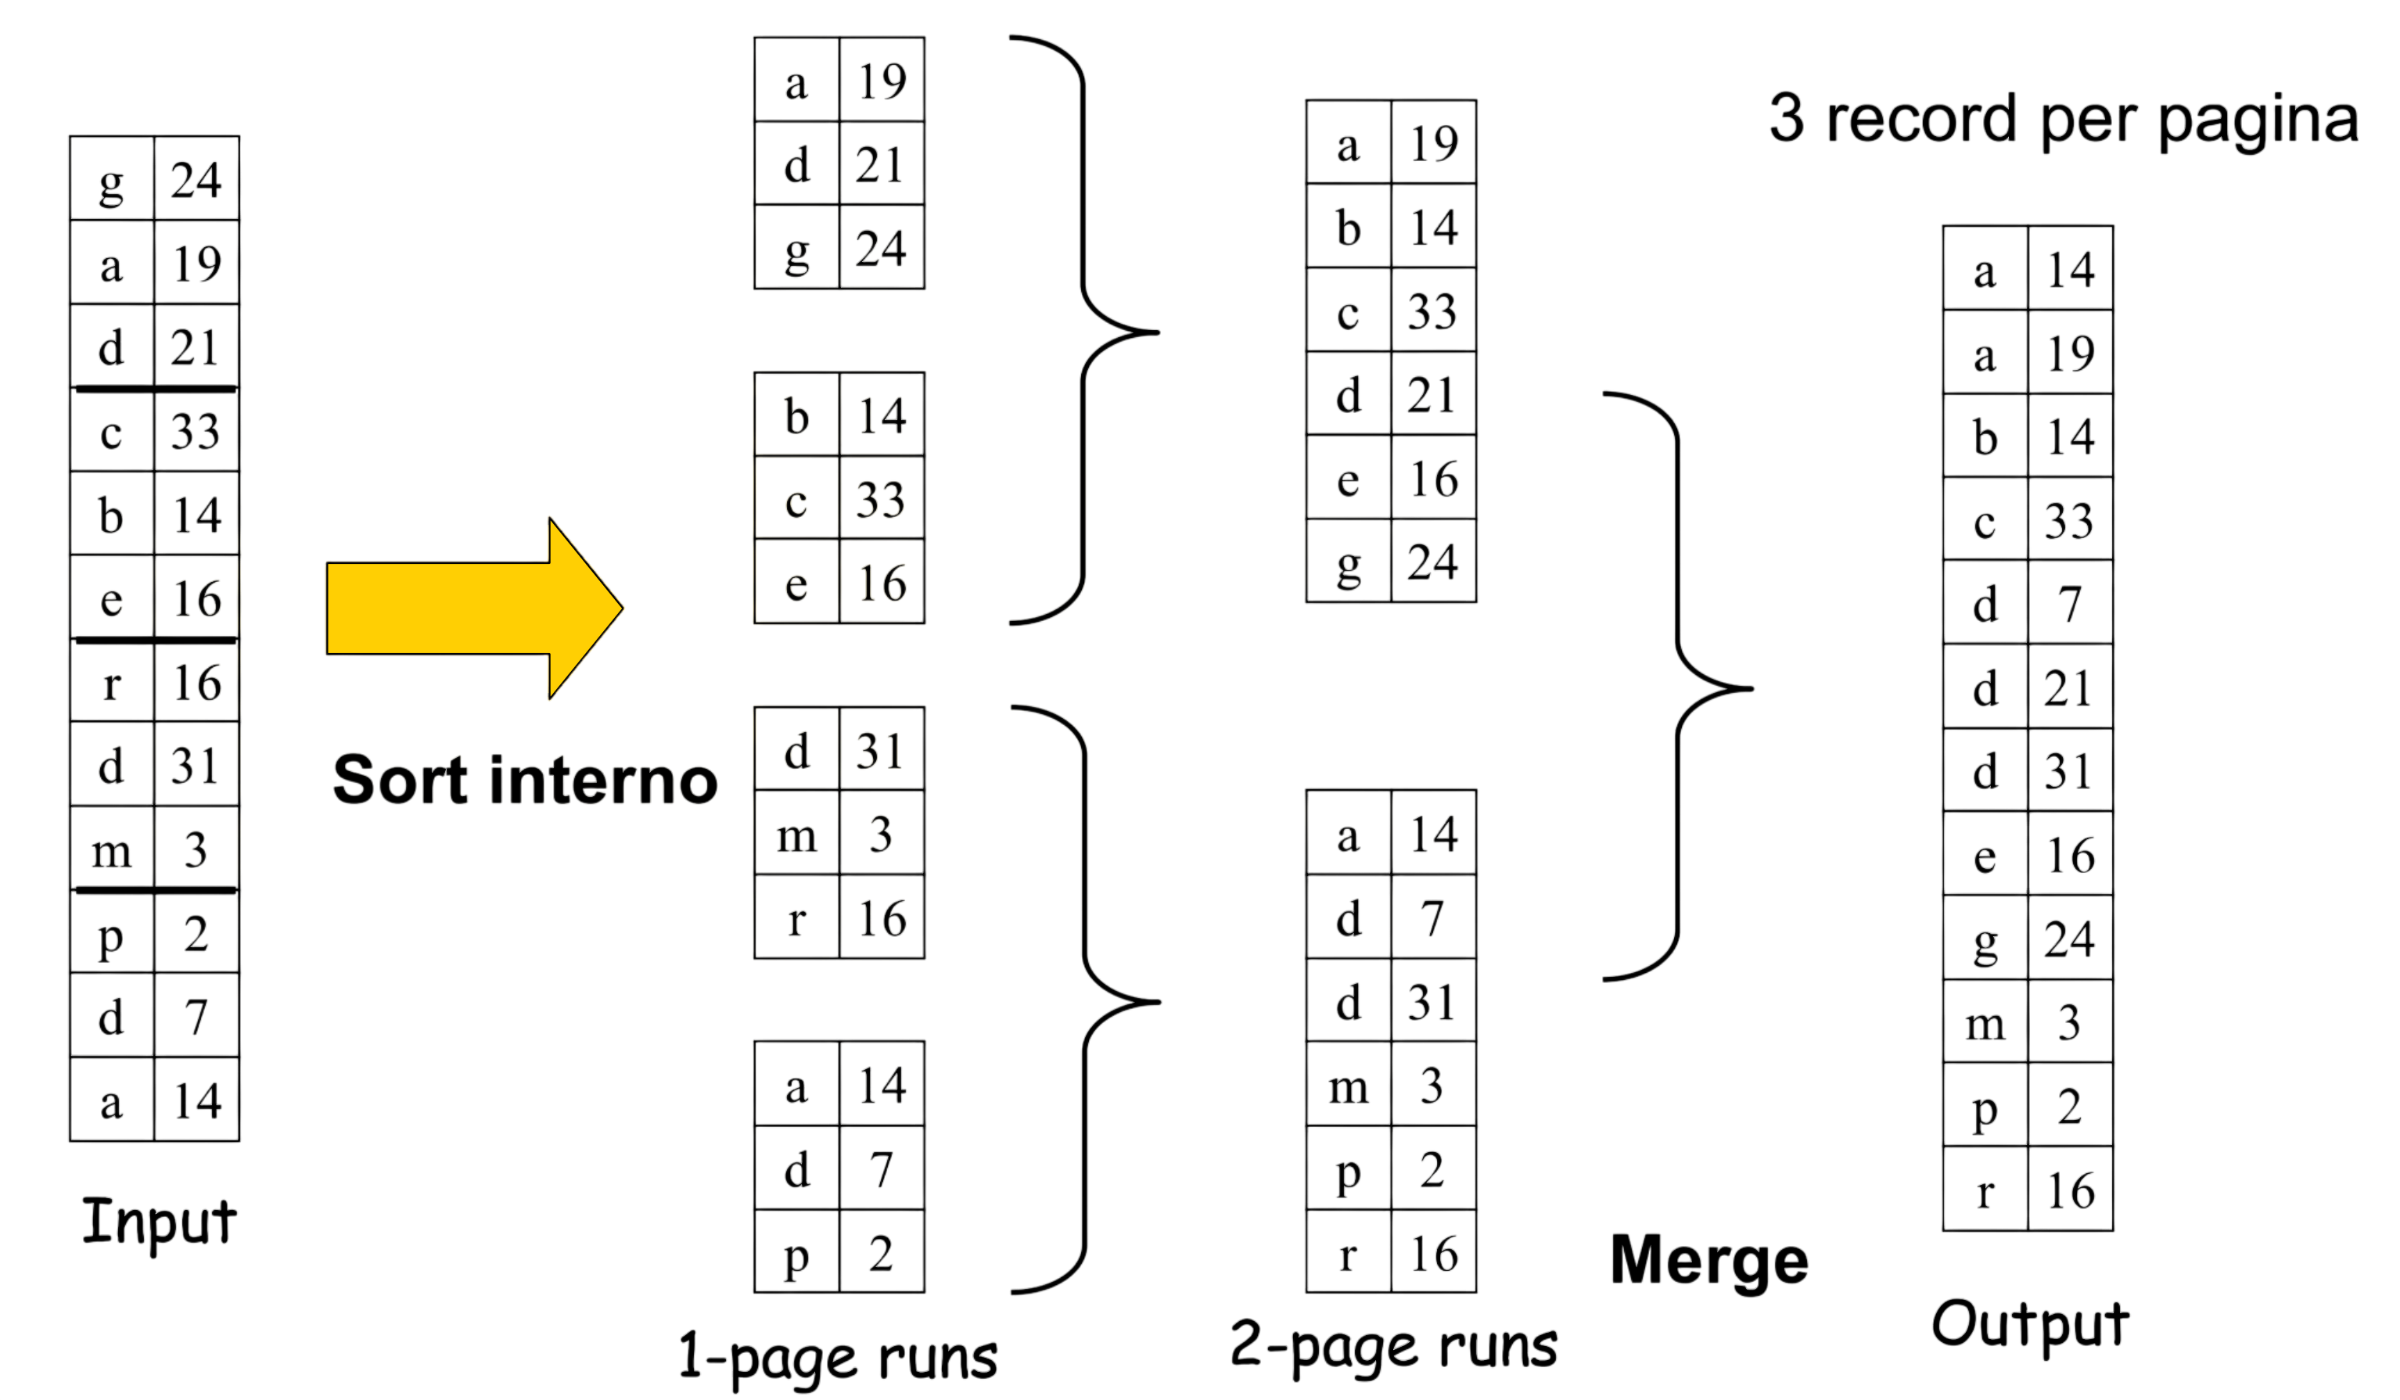
\includegraphics[width=0.6\textwidth]{images/ordinamento-Z-way-Sort-Merge.png}
    \end{figure}

    Durante il sort interno si carica e ordina una pagina alla volta ottenendo delle run ordinate.

    Si ottengono 4 run ordinate che passano alla fase di merge a due vie ($\mathrm{Z} = 2$) e si ottengono 2 run ordinate che passano ad un'ulteriore fase di merge, ottenendo così un'unica run ordinata.

    Con $\mathrm{NB} = 3$ si hanno solamente 3 buffer a disposizione, quindi, si associano 2 buffer alla run da passare alla fase di merge e 1 buffer per l'output.

    Si legge la prima pagina da ciascuna run e si genera la prima pagina dell'output, quando tutti i record di una pagina di run sono stati consumati, si legge un'altra pagina della run:
    \begin{figure}[H]
        \centering
        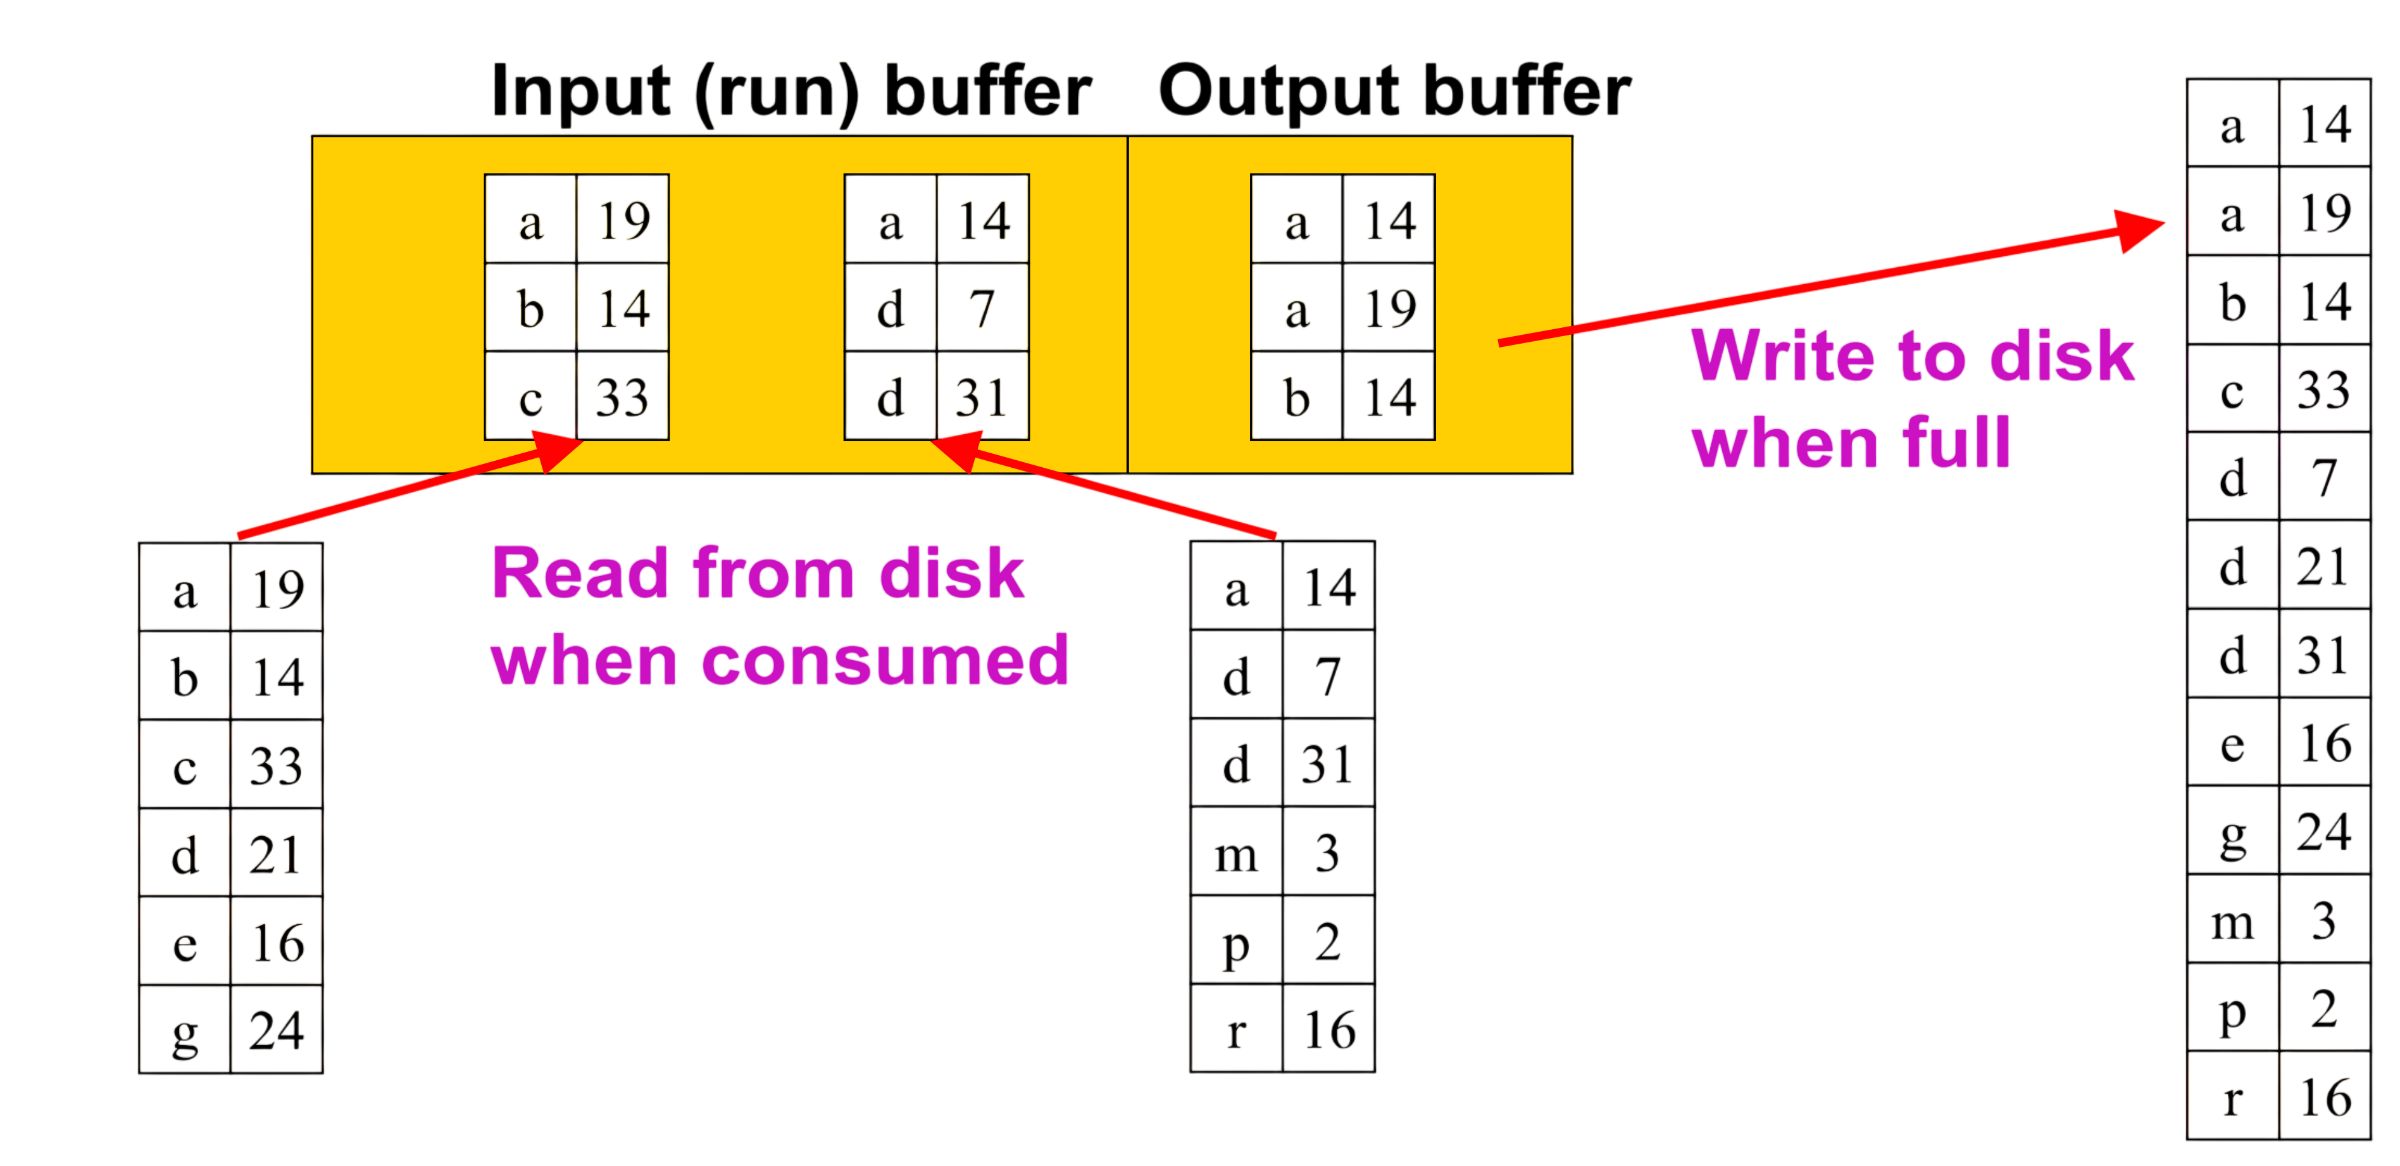
\includegraphics[width=0.6\textwidth]{images/utilizzoBuffer-Z-way-Sort-Merge.png}
    \end{figure}
}

\begin{itemize}[label=$\Rightarrow$, itemsep=\smallskipamount]
    \item \textcolor{red}{\textbf{costo ordinamento}} (con $\mathrm{Z} = 2$ e $\mathrm{NB} = 3$):
    \begin{itemize}[label=$\diamond$, itemsep=\smallskipamount]
        \item fase di sort interno: si leggono $\mathrm{NP(R)}$ pagine e si scrivono $\mathrm{NP(R)}$ pagine
        \[
            \mathrm{2 \cdot NP(R)}
        \]
        \item fase di merge: si leggono $\mathrm{NP(R)}$ pagine e si scrivono $\mathrm{NP(R)}$ pagine:
        \[
            \mathrm{2 \cdot NP(R)}
        \]
    \end{itemize}
    Il numero di passi di merge è:
    \[
        \mathrm{\lceil \log_2(NP(R)) \rceil}
    \]

    Il costo complessivo è:
    \[
        \mathbf{2 \times NP(R) \times (\lceil \log_2(NP(R)) \rceil)}
    \]
\end{itemize}

\subsection{Accesso diretto tramite indice}
Le interrogazioni che fanno uso dell'indice sono:
\begin{itemize}[label=$\diamond$, itemsep=\smallskipamount]
    \item \textbf{selezioni con condizione atomica di ugualianza} ($\mathrm{A = v}$): richiede indici di hash o B+ tree
    \item \textbf{selezione con condizione di range} ($\mathrm{A \geq v_1 \land A \leq v_2}$): richiede indice B+ tree
    \item \textbf{selezione con condizione costituita da una congiunzione di condizioni di ugualianza} ($\mathrm{A = v_1 \land B = v_2}$): l'indice viene scelto in base alla condizione più selettiva, l'altra condizione viene verificata filtrando i record restituiti dall'indice
    \item \textbf{selezioni con condizione costituita da una disgiunzione di condizioni di uguaglianza} ($\mathrm{A = v_1 \lor A = v_2}$): gli indici possono essere usati in parallelo e poi fare un merge o unione dei risultati
\end{itemize}

\subsection{Join}
Il join è l'operazione più costosa da eseguire, quindi, l'ottimizzatore è particolarmente attento ad ottimizzare questa operazione, tanto da prevedere diversi algoritmi:
\begin{itemize}[label=$\triangleright$, itemsep=\smallskipamount]
    \item \textbf{nested loop join}
    \item \textbf{merge scan join}
    \item \textbf{hash-based join}
\end{itemize}

Dal punto di vista logico il join è commutativo, ma dal punto di vista fisico c'è una differnza sostanziale tra $\mathbf{A \bowtie B}$ e $\mathbf{B \bowtie A}$ che cambia le prestazioni.

\subsubsection{Nested loop join}
Date 2 relazioni in input $\mathrm{R}$ e $\mathrm{S}$ tra cui è definito il predicato di join $\mathrm{PJ}$, distinguiamo:
\begin{itemize}[label=$\circ$, itemsep=\smallskipamount]
    \item \textbf{relazione esterna} $\mathbf{R}$
    \item \textbf{relazione interna} $\mathbf{S}$
\end{itemize}

L'algoritmo funziona come segue:
\begin{codiceSQL}
$\forall$ tupla $\mathrm{t_R}$ { --relazione esterna
    $\forall$ tupla $\mathrm{t_S}$ { --relazione interna
        if ($\mathrm{t_R, t_S}$) soddisfa PJ
            aggiungi ($\mathrm{t_R, t_S}$) al risultato
    }
}
\end{codiceSQL}

\esempio{algoritmo nested loop join}{
    Consideriamo il seguente esempio di join tra le relazioni $\mathrm{R}$ e $\mathrm{S}$:
    \begin{figure}[H]
        \centering
        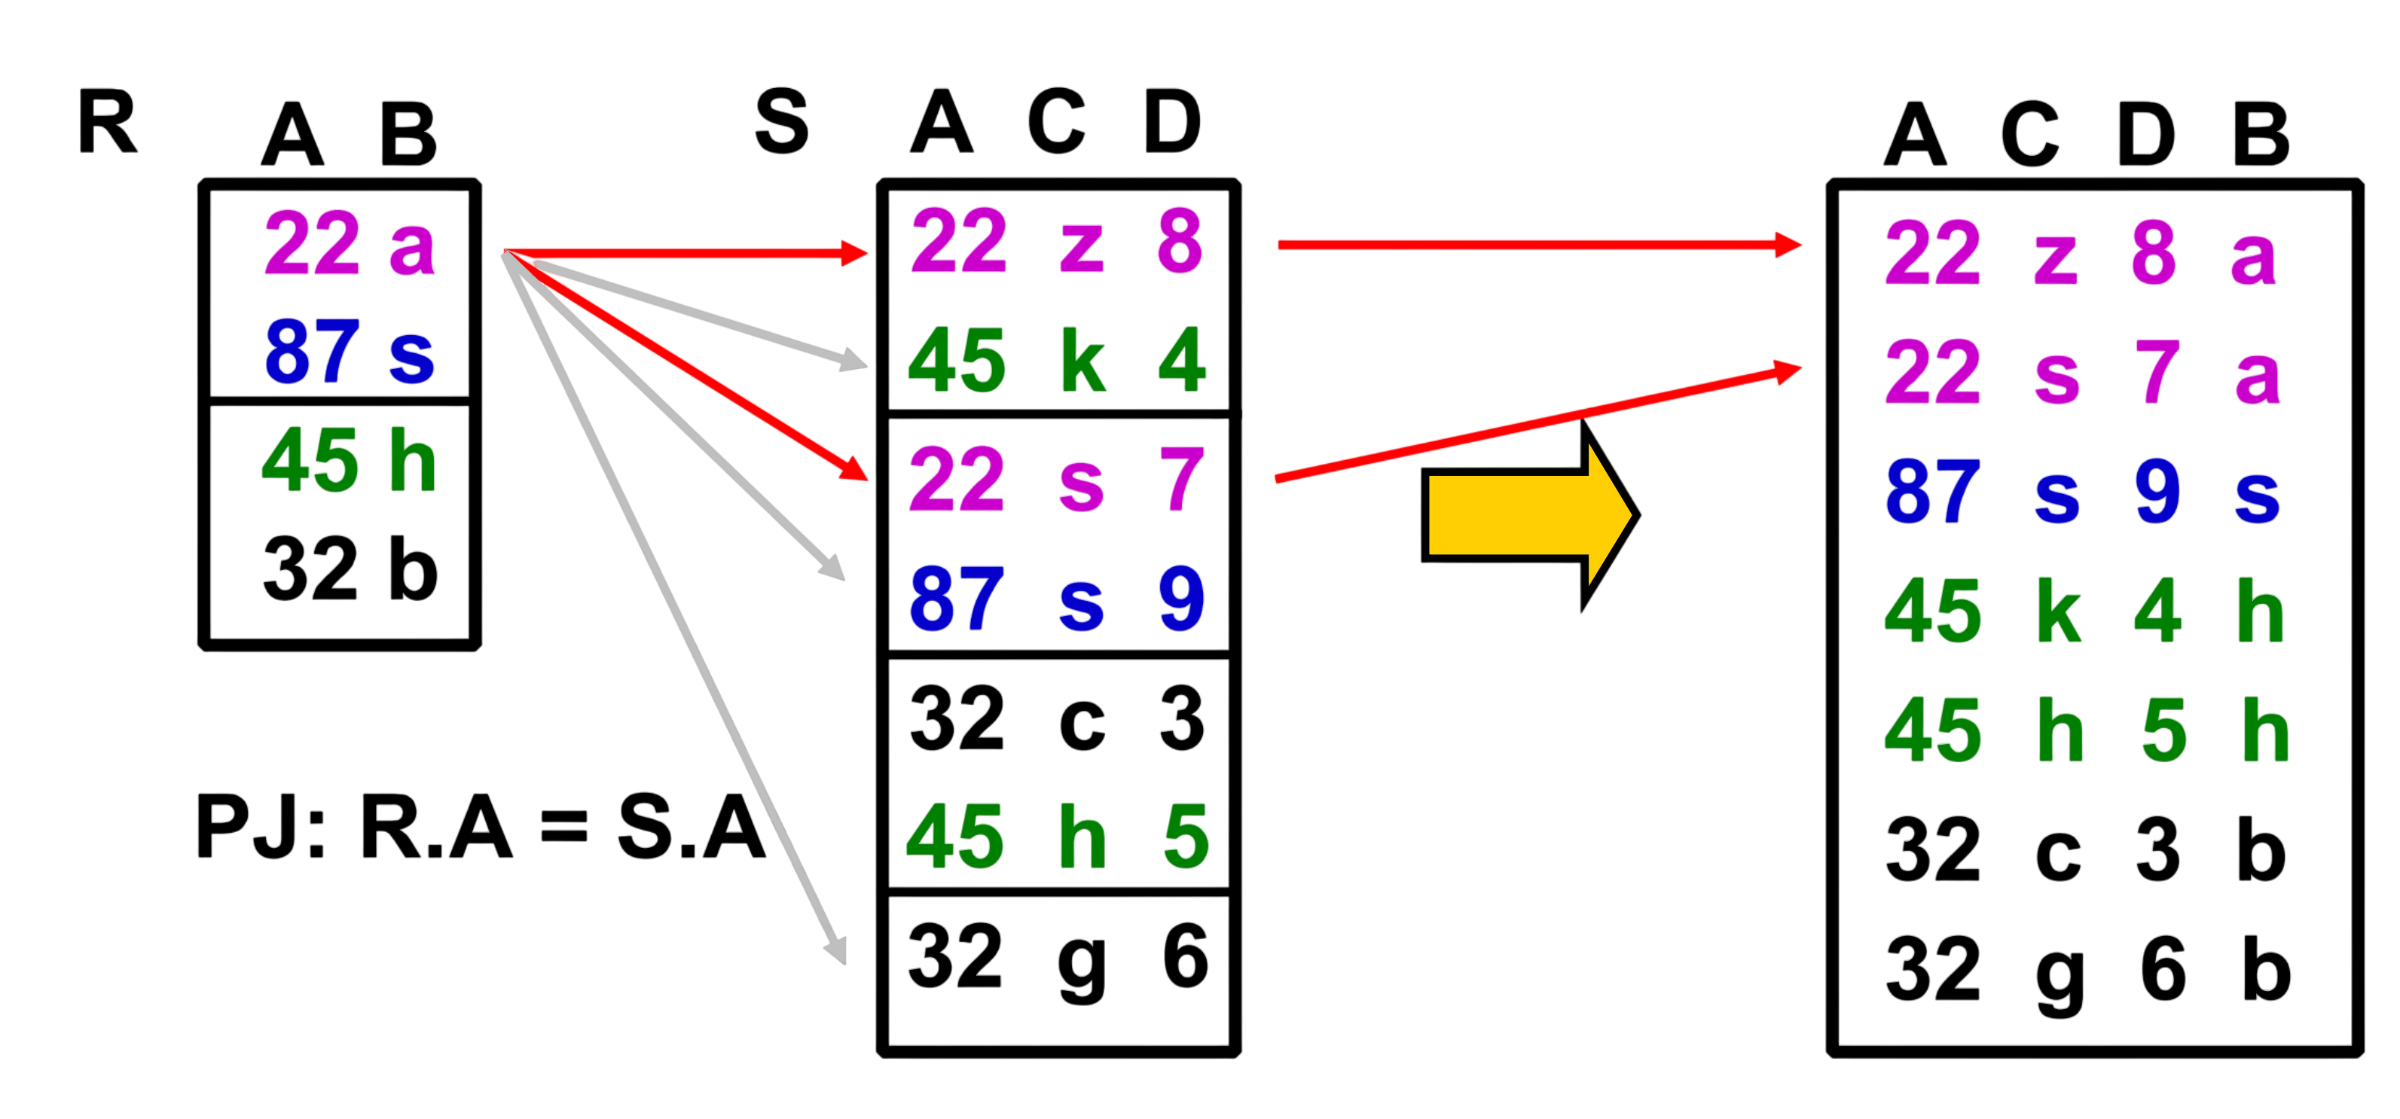
\includegraphics[width=0.5\textwidth]{images/nested-loop-join.png}
    \end{figure}

    $\mathrm{R}$ deve verificare per ogni riga di $\mathrm{S}$ che il predicato sia verificato.
}

\begin{itemize}[label=$\Rightarrow$, itemsep=\smallskipamount]
    \item \textcolor{red}{\textbf{costo nested loop join}} (consideriamo 1 pagina per caricare R e 1 pagina per caricare S):
    \begin{itemize}[label=$\diamond$, itemsep=\smallskipamount]
        \item bisogna leggere $\mathrm{R}$ completamente una volta
        \item per ogni riga di $\mathrm{R}$ ($\mathrm{NP(R) = \# \text{RIGHE R}}$) bisgona leggere completamente $\mathrm{S}$
    \end{itemize}

    \smallskip
    Il costo complessivo è:
    \[
        \mathbf{NP(R) + NR(R) \cdot NP(S)}
    \]
\end{itemize}

A seconda del numero di righe di $\mathrm{R}$ cambia il numero di volte che bisogna leggere $\mathrm{NP(R)}$, quindi, la relazione esterna deve essere quella più piccola per minimizzare il costo.

\subsubsection{Nested loop join con indice}
Data una relazione esterna $\mathrm{R}$ e una interna $\mathrm{S}$, si ha che la scansione completa di $\mathrm{S}$ può essere sostituita dalla scansione basata sull'indice costituito sugli attributi di join di $\mathrm{S}$.

\esempio{algoritmo nested loop join con indice}{
    Consieriamo il seguente esempio di nested loop join con indice tra le relazioni $\mathrm{R}$ e $\mathrm{S}$:
    \begin{figure}[H]
        \centering
        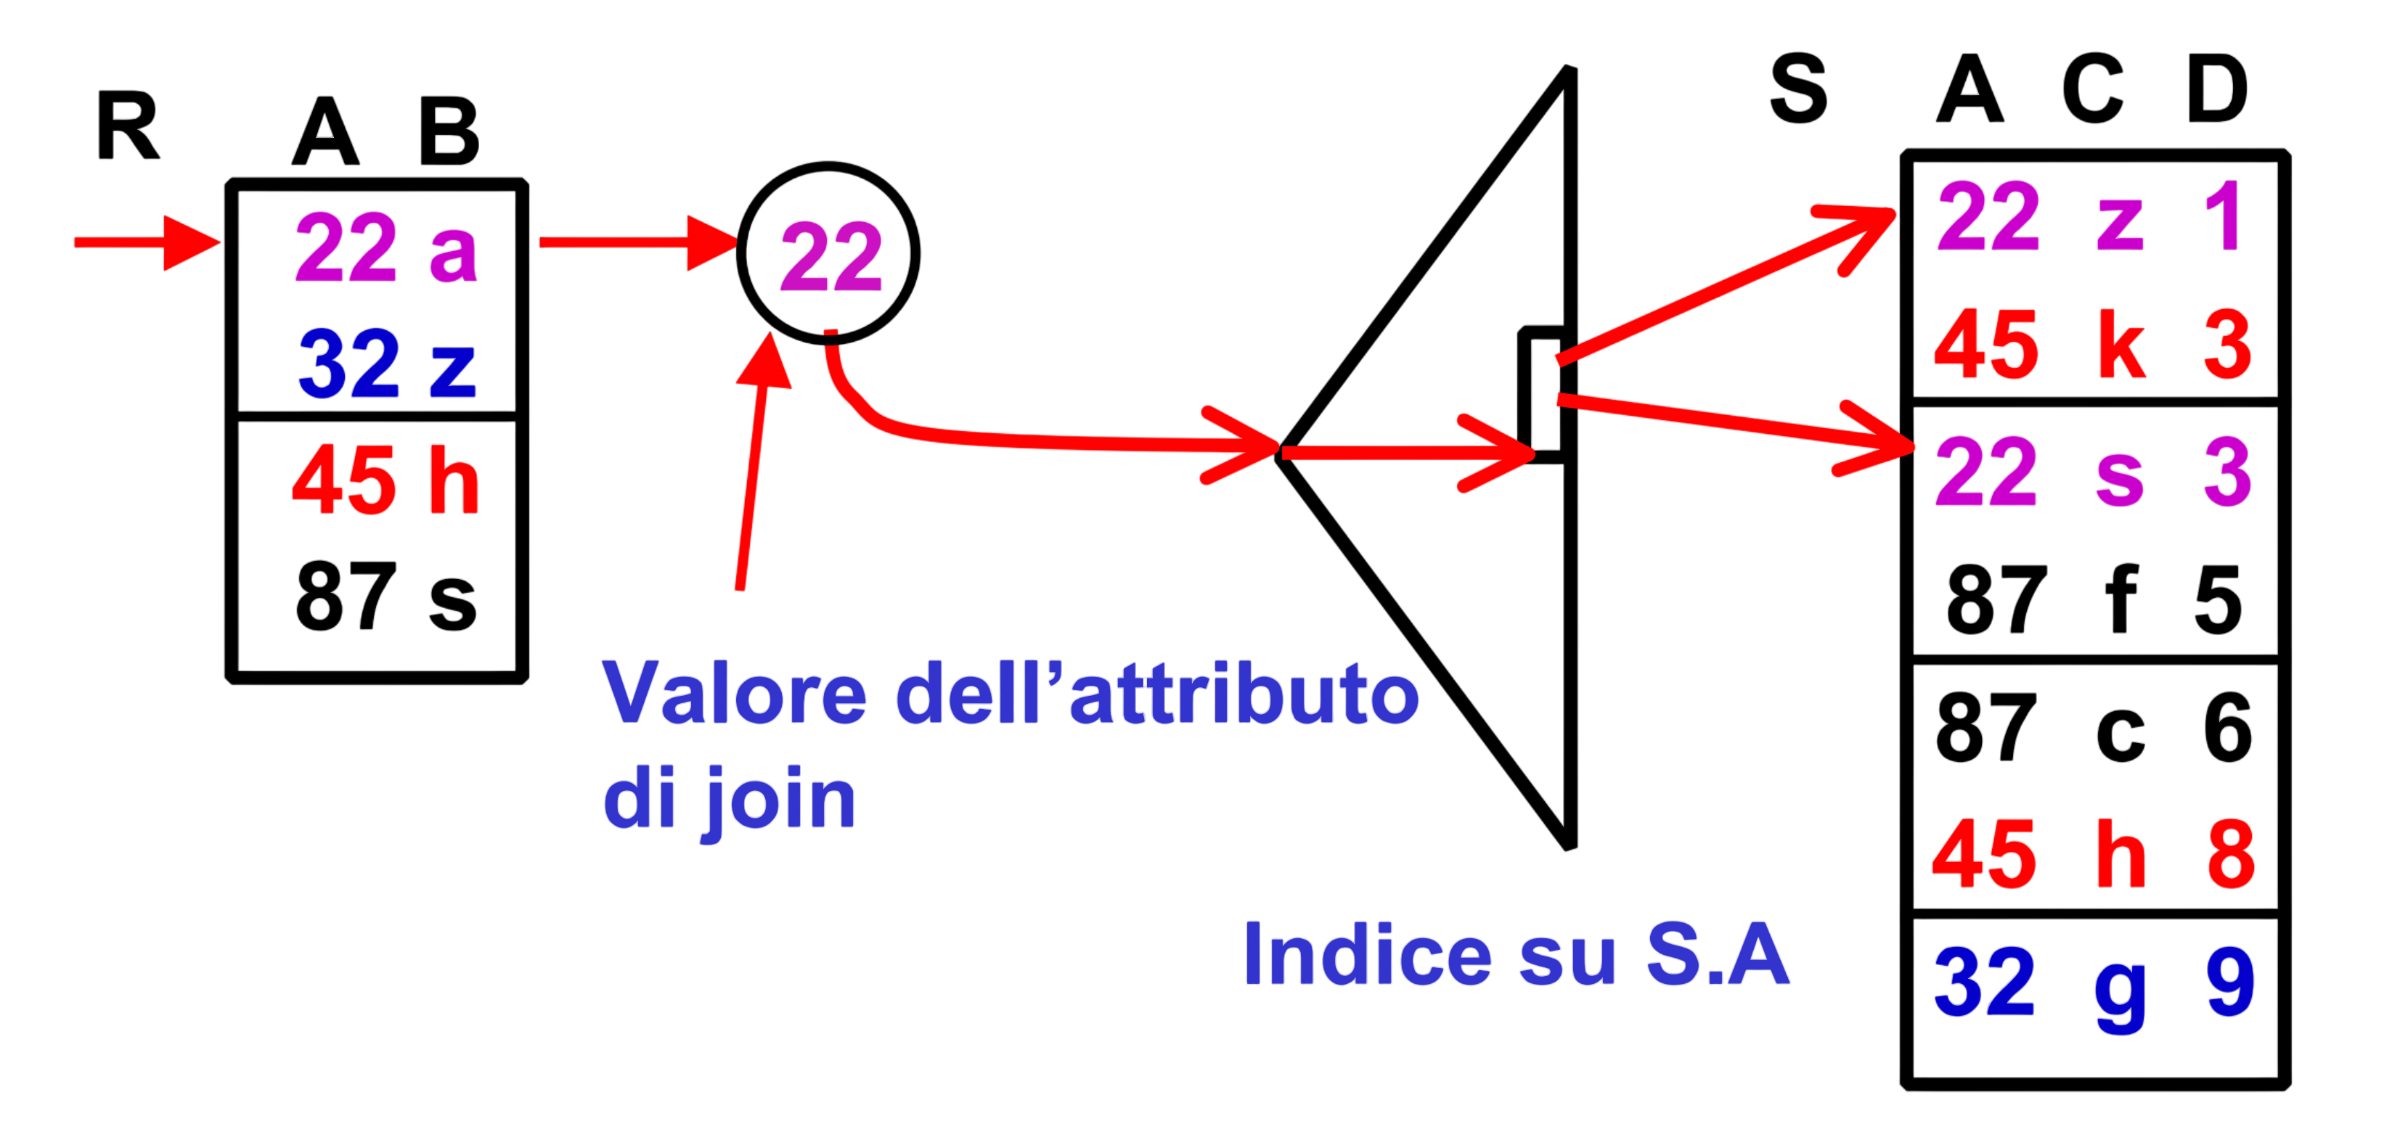
\includegraphics[width=0.5\textwidth]{images/nested-loop-join-indice.png}
    \end{figure}

    L'indice su $\mathrm{S.A}$ permette di caricare solo i blocchi di $\mathrm{S}$ che contengono l'attributo $\mathrm{A = 22}$.
}

\begin{itemize}[label=$\Rightarrow$, itemsep=\smallskipamount]
    \item \textcolor{red}{\textbf{costo nested loop join}} (usando B+ tree):
    \[
        \mathbf{NP(R) + NR(R)} \cdot \left(\text{ProfonditàIndice} + \mathbf{\frac{NR(S)}{VAL(A,S)}}\right)
    \]
\end{itemize}

La tabella $\mathrm{R}$ deve comunque essere caricata tutta ($\mathrm{NP(R)}$) e rimane invariato anche il numero di volte che si esegue il ciclo esterno ($\mathrm{NR(R)}$).\\[0.2ex]
Ciò che cambia è il numero di blocchi/pagine di $\mathrm{S}$ che si devono caricare tutte le pagine di ($\left(\text{ProfonditàIndice} + \mathrm{\frac{NR(S)}{VAL(A,S)}}\right)$).\\[0.2ex]
L'idea è, invece, di caricare tutte le pagine di $\mathrm{S}$ si caricano solo quelle che contengono $\mathrm{S.A = R.A}$
\begin{itemize}[label=$\diamond$, itemsep=\smallskipamount]
    \item $\mathbf{\frac{NR(S)}{VAL(A,S)}}$: rappresenta la stima di quanti blocchi di $\mathrm{S}$ contengono $\mathrm{A}$ uguale al valore interessato.
    
    Questa stima è anche chiamata \textbf{selettività} dell'attributo $\mathrm{A}$.
    \item $\mathbf{VAL(A,S)}$: numero di valori distinti di $\mathrm{A}$ che compaiono in $\mathrm{S}$
\end{itemize}

\esempio{}{
    Supponiamo che $\mathrm{A} = \text{Nome\_Regioni}$, quindi, il numero di possibili valori di $\mathrm{A}$ è 21.

    Consideriamo:
    \begin{itemize}[label=$\diamond$, itemsep=\smallskipamount]
        \item $\mathrm{NR(S) = 2100}$
        \item numero di righe per ogni regione è:
        \[
            \mathrm{\frac{NR(S)}{VAL(A,S)} = \frac{2100}{21} = 1000}
        \]

        quindi si ha l'assunzione che il dato sia unififorme, cioè che non siano più o meno lo stesso numero di pagine per ogni regione
        \item nel caso pessimo si ha un blocco/pagina per ogni riga
    \end{itemize}

    \smallskip
    Quindi, il costo del nested loop join con indice è:
    \[
        \begin{aligned}
            &\mathbf{NP(R) + NR(R)} \cdot \left(\text{ProfonditàIndice} + \mathbf{\frac{NR(S)}{VAL(A,S)}}\right)\\
            &\mathbf{NP(R) + NR(R) \cdot (\text{ProfonditàIndice} + 1000)}
        \end{aligned}
    \]
}

\subsubsection{Block nested loop join}
Il \textbf{block nested loop join} è una variante del nested loop in cui ciascuna pagina di $\mathrm{S}$ (tabella interna) viene letta per ogni pagina di $\mathrm{R}$ (tabella esterna), invece, che per ogni riga di $\mathrm{R}$.\\[0.2ex]
Lo pseudocodice è il seguente:
\begin{codiceSQL}
$\forall$ pagina $\mathrm{P_R}$ di R { --relazione esterna
    $\forall$ pagina $\mathrm{P_S}$ di S { --relazione interna
        $\forall$ tupla $\mathrm{t_R}$ di $\mathrm{P_R}$ {
            $\forall$ tupla $\mathrm{t_S}$ in $\mathrm{P_S}$ {
                if ($\mathrm{t_R}$ , $\mathrm{t_S}$) soddisfa PJ
                    aggiungi ($\mathrm{t_R}$ , $\mathrm{t_S}$) al risultato
            }
        }
    }
}
\end{codiceSQL}

\begin{itemize}[label=$\Rightarrow$, itemsep=\smallskipamount]
    \item \textcolor{red}{\textbf{costo block nested loop join}}: dipende dallo spazio a disposizione nei buffer.
    
    Supponiamo di avere 1 buffer per R e 1 buffer per S, allora:
    \begin{itemize}[label=$\diamond$, itemsep=\smallskipamount]
        \item bisogna leggere R completamente una volta, quindi NP(R)
        \item per ogni pagina di R (NP(R)) bisogna leggere completamente S quindi NP(R) NP(S)
    \end{itemize}

    \smallskip
    Il costo totale è:
    \[
        \mathbf{NP(R) + NR(R) \cdot NP(S)}
    \]
\end{itemize}

\esempio{algoritmo block nested loop join}{
    Consideriamo il seguente esempio di block nested loop join tra le relazioni R e S:
    \begin{figure}[H]
        \centering
        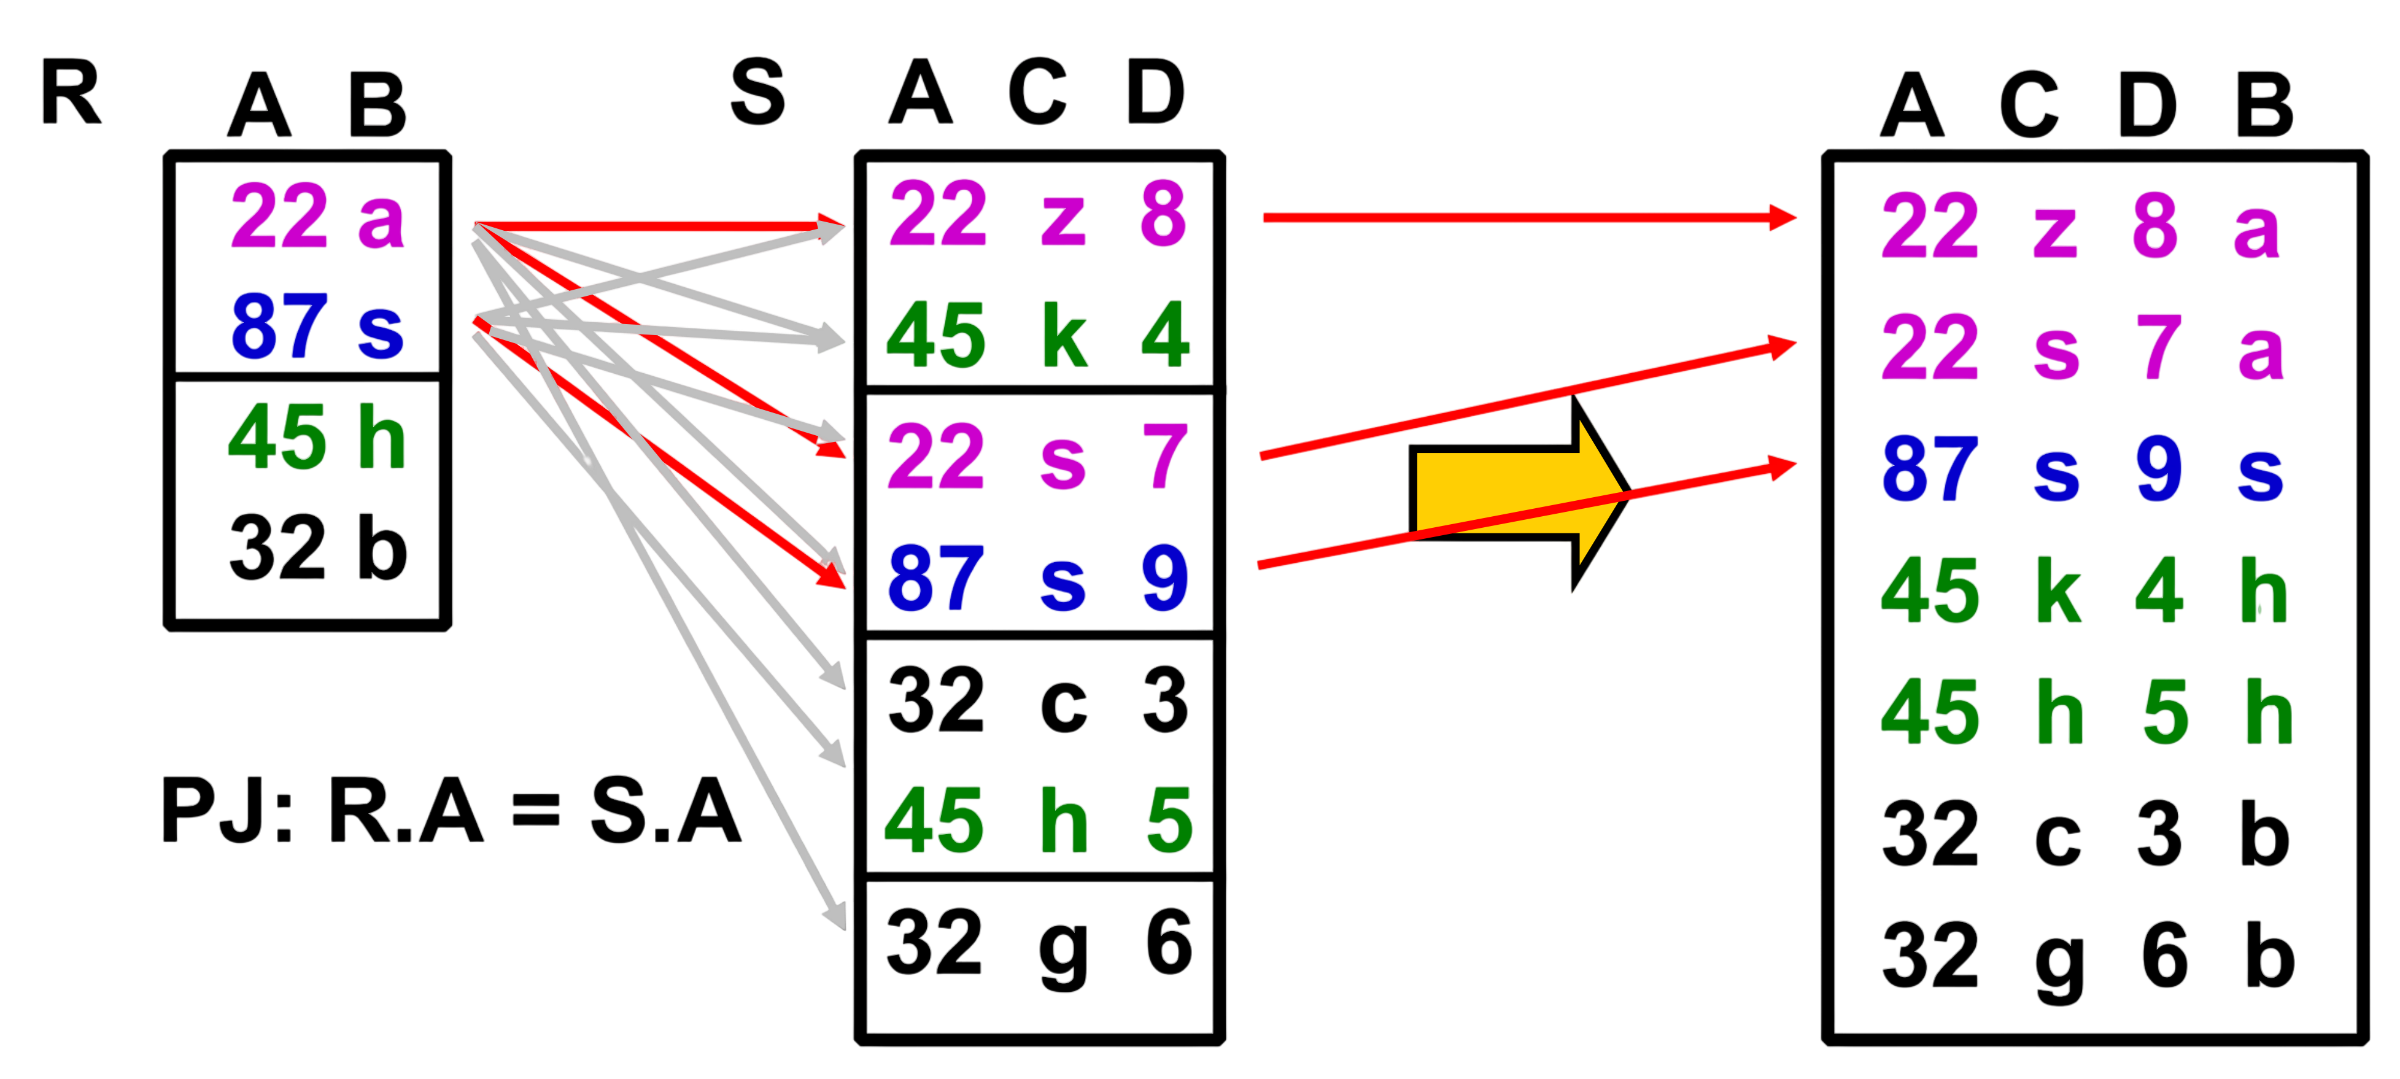
\includegraphics[width=0.5\textwidth]{images/block-nested-looop-join.png}
    \end{figure}
}

\subsubsection{Merge scan join}
Il \textbf{merge scan join} è applicabile quando entrambi gli insiemi di tuple in input sono ordinati sugli attributi di join e il join è un equi-join (predicato di join è una condizone di uguaglianza).\\[0.2ex]
Cià accade sia per entrambe le relazioni $\mathrm{R}$ e $\mathrm{S}$ vale almeno una delle seguenti condizioni:
\begin{itemize}[label=$\circ$, itemsep=\smallskipamount]
    \item relazione è fisicamente ordinata sugli attributi di join (file sequenziale ordinato come struttura fisica)
    \item esiste un indice sugli attributi di join della tabella che consente una scansione ordinata delle tuple
\end{itemize}

La logica di questo algoritmo sfrutta il fatto che entrambi gli input sono ordinati per evitare di fare confronti inutili e questo fa si che il numero di letture totali sia:
\[
    \mathbf{NP(R) + NP(S)}
\]

se si accede sequenzialmente alle due relazioni ordinate fisicamente.

\begin{itemize}[label=$\circ$, itemsep=\smallskipamount]
    \item con indici B+ tree su entrambe relazioni i costo può arrivare al massimo (con indici nel buffer) a:
    \[
        \mathbf{NR(R) + NR(S)}
    \]
    \item con una relazione ordinata e un solo indice il costo è al massimo:
    \[
        \mathbf{NP(R) + NR(S)} (\text{o viceversa})
    \]
\end{itemize}

\esempio{algoritmo merge scan join}{
    Consideriamo il seguente esempio di merge scan join tra le relazioni $\mathrm{R}$ e $\mathrm{S}$:
    \begin{figure}[H]
        \centering
        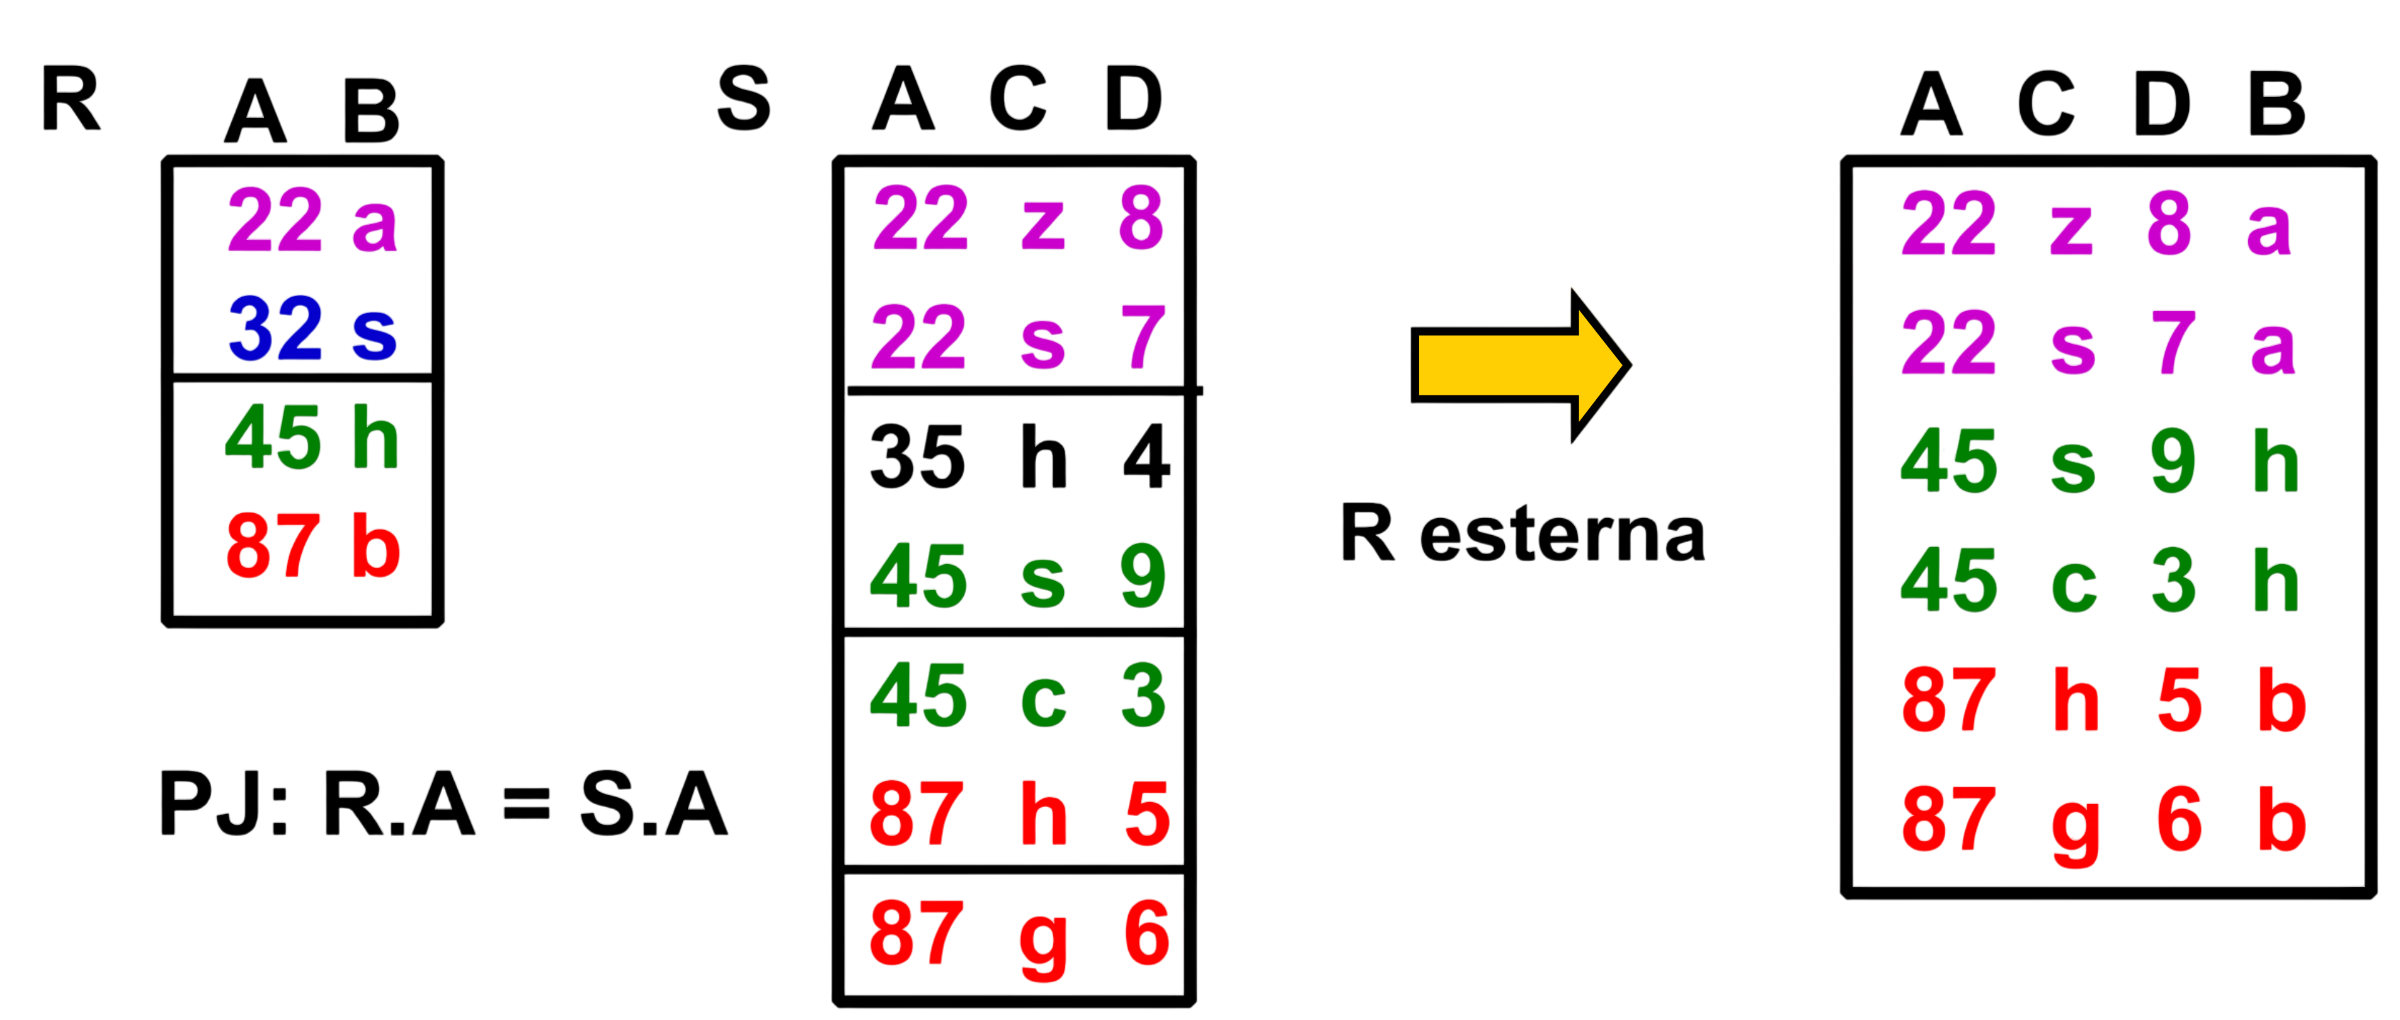
\includegraphics[width=0.5\textwidth]{images/merge-scan-join.png}
    \end{figure}
}

\subsubsection{Hash-based join}
L'algoritmo di \textbf{hash-based join} è applicabile solo in caso di equi-join e non richiede nè la presenza di indici nè input ordinati e risulta particolarmente vataggioso in caso di relazioni molto grandi.\\[0.2ex]
L'idea sui cui si basa l'hash join è semplice: si suppone di avere a disposizione una funzione hash $\mathrm{h}$ che viene applictaa agli attributi di join delle due relazioni (es. $\mathrm{R.J}$ e $\mathrm{S.J}$).

\begin{itemize}[label=$\circ$, itemsep=\smallskipamount]
    \item se $\mathrm{t_R}$ e $\mathrm{t_S}$ sono 2 tuple di $\mathrm{R}$ e $\mathrm{S}$, allora è possibile che sia $\mathrm{tR.J = tS.J}$ solo se $\mathrm{h(tR.J) = h(tS.J)}$
    \item se, viceversa, $\mathrm{h(tR.J) \neq h(tR.J)}$, allora si ha $\mathrm{tR.J \neq tS.J}$
\end{itemize}

Da questa idea si hanno diverse implementazioni, che hanno in comune il fatto che $\mathrm{R}$ e $\mathrm{S}$ vengono partizionate sulla base dei valori della funzione di hash $\mathrm{h}$, e che la ricerca di matching tuples aviene solo tra partizioni relative allo stesso valore di $\mathrm{h}$.

$\Rightarrow$ \textcolor{red}{\textbf{costo hash-based join}}:
\begin{itemize}[label=$\circ$, itemsep=\smallskipamount]
    \item costruzione dell'hash map:
    \[
        \mathbf{NP(R) + NP(S)}
    \]
    \item accesso alle matching tules che nel caso pessimo può costare:
    \[
       \mathbf{ NP(R) \cdot NP(S)}
    \]
\end{itemize}

\section{Scelta del piano esecuzione}
Data un'espressione ottimizzata in algebra, i passi da eseguire sono:
\begin{enumerate}[itemsep=\smallskipamount]
    \item \textbf{si generano tutti i possibili paini di esecuzione} (alberi) \textbf{alternativi} (o un sottoinsieme) \textbf{ottenuti considernando le seguenti dimensioni}
    \begin{itemize}[label=$\circ$, itemsep=\smallskipamount]
        \item operatori alternativi applicabili per l'accesso ai dati: scan sequenziale o via indice
        \item operatori alternativi applicabili nei nodi: nested loop join o hash based join
        \item ordine delle operazioni da compiere (associatività)
    \end{itemize}
    \item \textbf{si valuta con formule approssimate il costo di ogni alternativa in termini di accessi alla memoria secondaria richiesti} (è una stima)
    \item \textbf{si sceglie l'albero con il costo stimato minimo}
\end{enumerate}

Nella valutazione delle stime di costo si tiene conto del profilo delle relazioni, solitamente memorizzato nel data directory e contente per ogni relazione $\mathrm{T}$:
\begin{itemize}[label=$\circ$, itemsep=\smallskipamount]
    \item stima della cardinailtà (\# tuple): $\mathrm{CARD(T)}$
    \item stima della dimensione di una tupla: $\mathrm{SIZE(T)}$
    \item stima della dimensione di ciascun attributo $\mathrm{A}$: $\mathrm{VAL(A,T)}$
    \item stima del numero di valori distinti per ogni attributo $\mathrm{A}$: $\mathrm{MAX(A,T)}$ e $\mathrm{MIN(A,T)}$
\end{itemize}

\begin{esempiobox}{Esercizio}
    Consideriamo la seguente base di dati:
    \[
        \begin{aligned}
            &\texttt{INGREDIENTE(\underline{codice}, nome, calorie)}\\
            &\texttt{COMPOSIZIONE(\underline{ricetta, ingrediente}, quantità)}\\
            &\texttt{RICETTA(\underline{codiceRicetta}, nome, regione, tempoPreparazione)}
        \end{aligned}
    \]

    e i seguenti vincoli d'integrità:
    \[
        \begin{aligned}
            &\text{Composizione.ricetta} \rightarrow \text{Ricetta}\\
            &\text{Composizione.ingrediente} \rightarrow \text{Ingrediente}
        \end{aligned}
    \]

    Data la seguente query:
\begin{codiceSQL}
SELECT R.codiceRicetta, I.nome, I.calorie
FROM RICETTA R
JOIN Composizione C ON R.codiceRicetta = C.ricetta
JOIN Ingrediente I ON C.Ingrediente = I.codice
    WHERE R.regione = 'Veneto';
\end{codiceSQL}

    \textcolor{red}{\textbf{Calcolare il costo dell'interrogazione in termini di numero di accessi alla memoria sedcondaria con le seguenti ipotesi:}}
    \begin{itemize}[label=$\circ$, itemsep=\smallskipamount]
        \item la selezione (\texttt{R.Veneto = 'Veneto'}) su \texttt{Riccetta} richiede una scansione sequenziale della tabelle \texttt{Ricetta}.
        
        Inoltre, la selezione rimane nel buffer.
        \item l'ordine di esecuzione del join è:
        \[
            (\text{Ricetta} \Join \text{Composizione}) \Join \text{Ingrediente}
        \]
        \item le operazioni di join vengono eseguite con la tecnica nested loop join con 1 pagina di buffer a disposizione per ogni tabella
        \item il risultato del primo join ($\text{Ricetta} \Join \text{Composizione}$) viene interamente mantenuto nel buffere
        \item il numero di pagine e righe per ogni tabella è il seguente:
        \begin{table}[H]
            \centering
            \begin{tabular}{|c|c|c|c|c|c|}
                \hline
                Tabella & NP & NR & VAL(regione) & VAL(Ricetta) & VAL(Qtà)\\
                \hline
                Ingrediente & 30 & 270 & & & \\
                Composizione & 780 & 19800 & & 90 & 50\\
                Ricetta & 150 & 900 & 18 & \\
                \hline
            \end{tabular}
        \end{table}
    \end{itemize}

    \textbf{Svolgimento}
    \begin{enumerate}[itemsep=\medskipamount]
        \item \textbf{selezione su ricetta}:
        \item \textbf{join su Composizione}:
        \item \textbf{join su Ingrediente}:
    \end{enumerate}
\end{esempiobox}


    %!TeX root = BasiDiDati.tex

\chapter{Laboratorio}
PostgreSQL è un \textcolor{azzurrino}{\textbf{R}}elational \textcolor{azzurrino}{\textbf{D}}ata \textcolor{azzurrino}{\textbf{B}}ase \textcolor{azzurrino}{\textbf{M}}anagement \textcolor{azzurrino}{\textbf{S}}ystem con alcune funzionalità orientate agli oggetti.

L'interazione tra un utente (programmatore/utente finale) e le basi di dati gestite da PostgreSQL avviene secondo il modello client-server.

\begin{figure}[H]
  \centering
  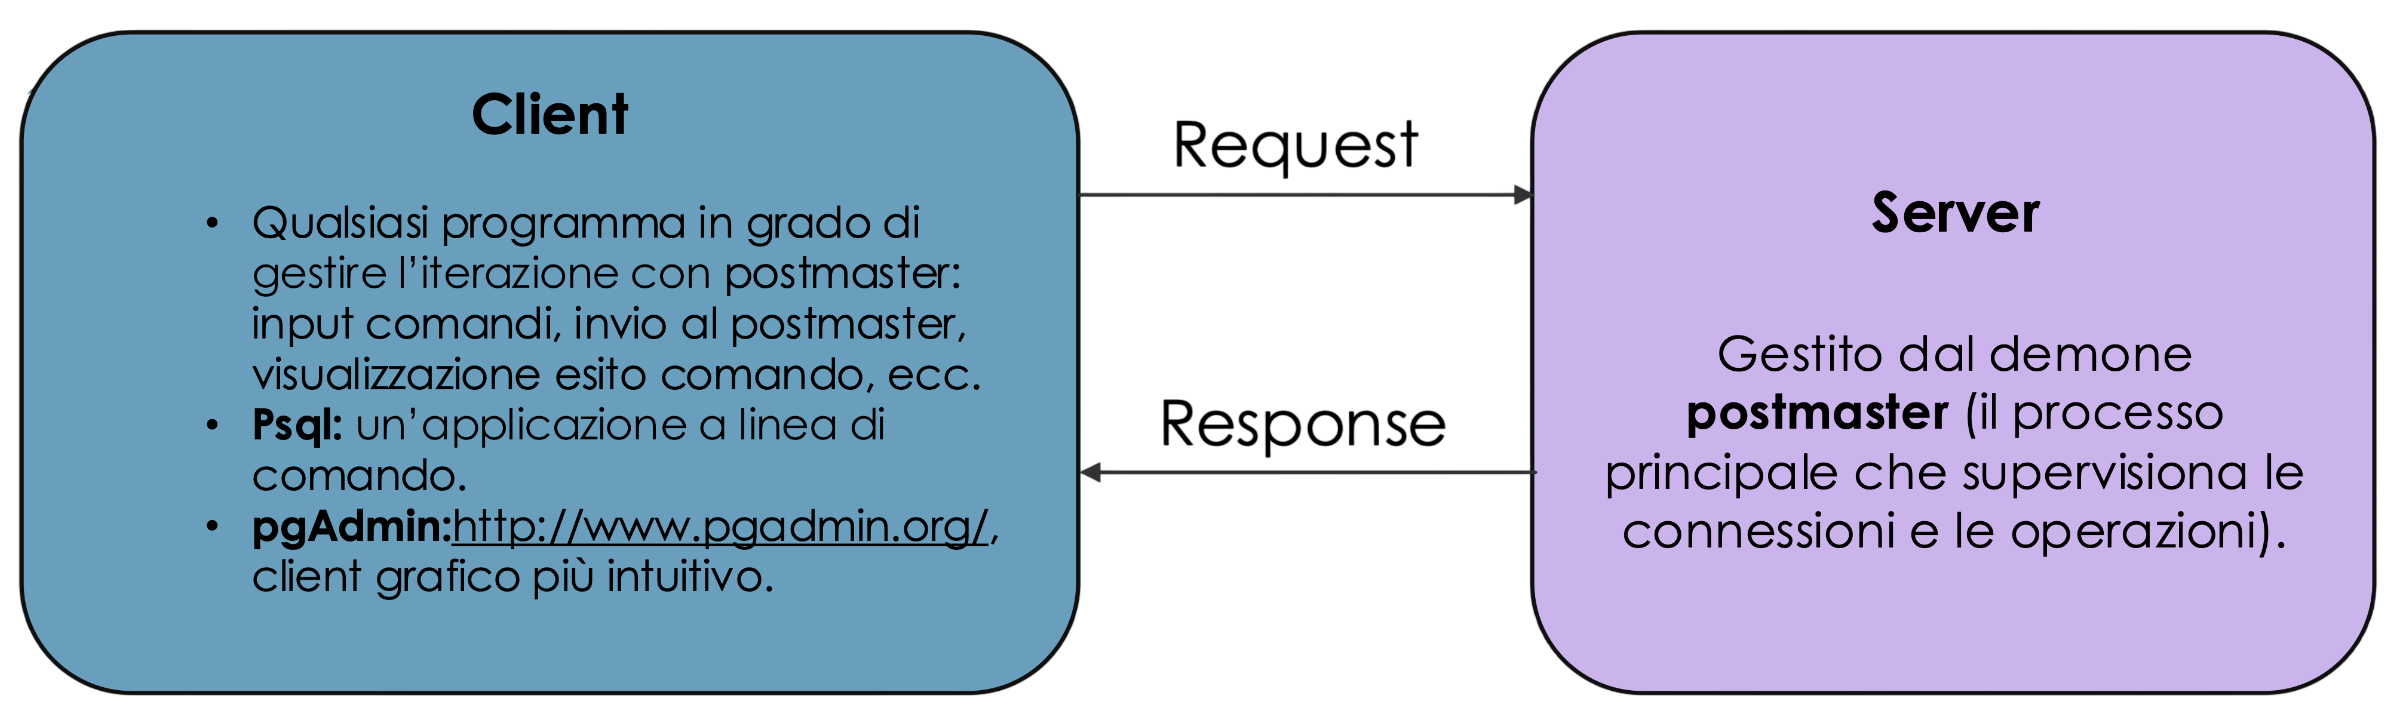
\includegraphics[width=0.8\textwidth]{images/ClientServer.png}
\end{figure}

\section{Comando \protect\texttt{CREATE TABLE}}
Il comando $\verb|CREATE TABLE|$ definisce uno schema di relazione e ne crea un'istanza vuota, specificando attributi, domini e vincoli.

La sintassi è:
\begin{codiceSQL}
CREATE TABLE tabella(
  attributo dominio [valoreDefault] {vincolo},
  attributo dominio [valoreDefault] {vincolo},
  {vincoloTabella}
);
\end{codiceSQL}

dove:
\begin{itemize}[label=$\triangleright$, itemsep=\smallskipamount]
  \item $\verb|[]|$: indicano parti opzionali
  \item $\verb|[valoreDefault]|$: indica un eventuale valore di default
  \item $\verb|{}|$: indica un elemento che può essere ripetuto 0 o più volte
  \item $\verb|{vincolo}|$: indica eventuali (0 o più) vincoli per ogni attributo
\end{itemize}

\begin{esempiobox}{Utilizzo di \texttt{CREATE TABLE}}
\begin{codiceSQL}
CREATE TABLE Impiegato (
  Matricola CHARACTER(6) PRIMARY KEY, 
  Nome VARCHAR(20) NOT NULL, 
  Cognome VARCHAR(20) NOT NULL,
  Dipart VARCHAR(15), 
  Stipendio NUMERIC(9) DEFAULT 0,
  FOREIGN KEY(Dipart) 
    REFERENCES Dipartimento(NomeDip),     -- vincolo di tabella
  UNIQUE (Cognome,Nome)                   -- vincolo di tabella
);
\end{codiceSQL}
\end{esempiobox}

\subsection{Identificatori}
\definizione{identificatore}{
  Un \textbf{identificatore} è una sequenza di caratteri che identifica un elemento del database (tabella, attributo, vincolo, ecc.).
}

Gli identificatori, in SQL, devono rispettare alcune regole:
\begin{itemize}[label=$\diamond$, itemsep=\smallskipamount]
  \item iniziare con una lettera (UTF-8) o un underscore (\_)
  \item possono contenere lettere, numeri (0-9) o underscore (\_)
  \item non possono essere parole chiave riservate a SQL
\end{itemize}

\vario{Nota}{
  Gli identificatori \textbf{non sono case sensitive}! (\texttt{idPersona} = \texttt{idpersona})
}

\subsection{Domini elementari}
\definizione{domini elementari}{
  I domini elementari (predefiniti) sono:
  \begin{itemize}[label=$\triangleright$, itemsep=\smallskipamount]
    \item \textbf{caratteri}: singoli caratteri o stringhe anche di lunghezza variabile
    \item \textbf{bit}: bit singoli (booleani) o stringhe di bit
    \item \textbf{numeri esatti e approssimati}
    \item \textbf{istanti temporali}
    \item \textbf{intervalli temporali}
  \end{itemize}
}

\subsubsection{Tipo carattere}
Permette di rappresentare singoli caratteri oppure stringhe.

Un carattere o stringa di caratteri sono rappresentati tra apici ('):
\texttt{'a'}, \texttt{'Questa è una stringa'}.

La sintassi è:
\begin{codiceSQL}
CHARACTER [VARYFING] [(lunghezza)]
\end{codiceSQL}

dove:
\begin{itemize}[label=$\triangleright$]
  \item $\verb|lunghezza|$: può essere fissa o variabile
  \begin{itemize}[label=$\diamond$, itemsep=\medskipamount]
    \item $\verb|CHARACTER|$: carattere singolo
    \item $\verb|CHARACTER(20)|$: stringa di lunghezza fissa (20 caratteri).
    
    Se la stringa è più corta di 20 caratteri, viene riempita con spazi a destra
    \item $\verb|CHARACTER VARYFING(20)|$ o $\verb|VARCHAR(20)|$: stringa di lunghezza variabile (max. 20 caratteri)
    \item $\verb|TEXT|$: stringa di lunghezza variabile senza limite fissato
  \end{itemize}
\end{itemize}

\subsubsection{Tipo boolean}
Permette di rappresentare valori booleani (\texttt{true} o \texttt{false}), più lo stato nullo.

La sintassi è:
\begin{codiceSQL}
BOOLEAN
\end{codiceSQL}

La rappresentazione dei valori booleani può essere:
\begin{itemize}[label=$\circ$, itemsep=\smallskipamount]
  \item $\verb|TRUE|$ o $\verb|FALSE|$
  \item $\verb|t|$ o $\verb|f|$
  \item $\verb|1|$ o $\verb|0|$
  \item $\verb|yes|$ o $\verb|no|$
  \item $\verb|NULL|$
\end{itemize}

\subsubsection{Tipo numerico esatto}
Permettono di rappresentare valori esatti (interi o con una parte decimale di lunghezza prefissata):
\begin{itemize}[label=$\triangleright$, itemsep=\medskipamount]
  \item \textbf{valori interi}:
  \begin{itemize}[label=$\diamond$, itemsep=\smallskipamount]
    \item $\verb|SMALLINT|$: valori interi (2 bytes: da -32.768 (215) a +32.767 (215-1))
    \item $\verb|INTEGER|$: valori interi (4 bytes: da -2147483648 (231) to +2147483647 (231-1))
  \end{itemize}
  \item \textbf{valori decimali}:
  \begin{itemize}[label=$\diamond$, itemsep=\smallskipamount]
    \item $\verb|NUMERIC [(precisione [, scala])]|$:
    \begin{itemize}[label=$\circ$, itemsep=\smallskipamount]
      \item $\verb|precisione|$: numero totale di cifre significative (cifre a sinistra e a destra della virgola)
      \item $\verb|scala|$: numero di cifre dopo la virgola (vuoto = 0)
    \end{itemize}
  \item $\verb|DECIMAL [(precisione [, scala])]|$: equivalente al precedente
  \end{itemize}
\end{itemize}

\esempio{tipo numerico esatto}{
  \texttt{NUMERIC(5,2)} permette di rappresentare valori come 100.01, 100.999 (arrotondato a 101.00), ma non valori come 1000.01
}

\subsubsection{Tipo numerico approssimato}
Permettono di rappresentare valori in virgola mobile:
\begin{itemize}[label=$\diamond$, itemsep=\smallskipamount]
  \item $\verb|REAL|$: precisione di 6 cifre decimali
  \item $\verb|DOUBLE PRECISION|$: precisione di 15 cifre decimali
\end{itemize}

\smallskip
Ciascun numero è rappresentato da una coppia di valori: \textbf{mantissa} (numero frazionario) + \textbf{esponente} (numero intero).\\[0.2ex]
Il valore si ottiene moltiplicando la mantissa per la potenza di 10 con grado pari all'esponente:
\begin{itemize}[itemsep=\smallskipamount]
  \item numero 0.17E16 corrisponde a $1,7 \times 10^{15}$
  \item numero -0.4E-6 corrisponde a $-4 \times 10^{-7}$
\end{itemize}

\subsubsection{Istanti temporali}
Permettono di rappresentare istanti di tempo.
\begin{itemize}[label=$\diamond$, itemsep=\medskipamount]
  \item $\verb|DATE|$: istanti del tipo (anno, mese, giorno)
  
  Si rappresenta tra apici (es. $\verb|'2025-12-01'|$) e lo standard ISO prescrive il formato \texttt{YYYY-MM-DD}
  \item $\verb|TIME [(precisione)][WITH TIME ZONE]|$: istanti del tipo (hour, minute, second)
  \begin{itemize}[itemsep=\smallskipamount]
    \item $\verb|precisione|$: numero cifre decimali per rappresentare frazioni del secondo
    \item $\verb|WITH TIME ZONE|$: permette di specificare anche [+-] hour: minute, che rappresentano la differenza con l'ora di Greenwich, o nomeFusoOrario
  \end{itemize}
  \item $\verb|TIMESTAMP [(precisione)][WITH TIME ZONE]|$: date + time
\end{itemize}

\subsubsection{Intervalli temporali}
Rappresenta un intervallo di tempo.

La sintassi è:
\begin{codiceSQL}
INTERVAL PrimaUnitaTempo [TO UltimaUNitaTempo]
\end{codiceSQL}

dove:
\begin{itemize}[label=$\triangleright$]
  \item $\verb|PrimaUnitàDiTempo|$ e $\verb|UltimaUnitàDiTempo|$: definiscono le unità di misura che devono essere utilizzate, dalla più precisa alla meno precisa
\end{itemize}

L'insieme delle unità di misura è diviso in due insiemi distinti:
\begin{itemize}
  \item Year-Month
  \item Day-Hour–Minute-Second
\end{itemize}

\subsection{Domini definiti dall'utente}
Per creare un dominio si esegue il comando:
\begin{codiceSQL}
CREATE DOMAIN nome AS tipoBase [valoreDefault][vincolo]
\end{codiceSQL}

dove:
\begin{itemize}[label=$\triangleright$]
  \item $\verb|CREATE DOMAIN|$: definisce un dominio, utilizzabile in definizioni di relazioni, anche con vincoli e valori di default
\end{itemize}

Il dominio può essere definito a partire da un dominio elementare oppure da un altro dominio definito dall'utente.

\begin{esempiobox}{Comando \texttt{CRETATE DOMAIN}}
\begin{codiceSQL}
CREATE DOMAIN giorniSettimana AS CHARACTER(3)
 CHECK(VALUE IN('LUN', 'MAR', 'MER', 'GIO', 'VEN', 'SAB', 'DOM'));

CREATE DOMAIN Voto AS SMALLINT DEFAULT NULL
 CHECK (value >= 18 AND value <= 30);
\end{codiceSQL}
\end{esempiobox}

\subsection{Vincoli intrarelazionali}
I vincoli intrarelazionali sono vincoli che si applicano a livello di relazione, cioè a una singola tabella.

I principali vincoli intrarelazionali sono:
\begin{itemize}[label=$\diamond$, itemsep=\medskipamount]
  \item $\verb|NOT NULL|$: valore nullo non è ammesso per l'attributo, quindi il valore deve sempre essere specificato, o si assegna un valore di default
  \item $\verb|UNIQUE|$: definisce (super)chiavi
\begin{codiceSQL}
Nome VARCHAR(20),
Cognome VARCHAR(20),
UNIQUE(Nome, Cognome)
--impone che non ci siano due righe che abbiano uguale
--sia il nome che il cognome
\end{codiceSQL}

\begin{codiceSQL}
Nome VARCHAR(20) UNIQUE,
Cognome VARCHAR(20) UNIQUE
--impone che non ci siano due righe che abbiano lo stesso nome
--o lo stesso cognome 
\end{codiceSQL}
  \item $\verb|PRIMARY KEY|$: chiave primaria (una sola, implica \texttt{NOT NULL}) 
\begin{codiceSQL}
matricola CHAR(6) PRIMARY KEY;
--se unico componente della chiave primaria
\end{codiceSQL}

\begin{codiceSQL}
nome VARCHAR(20),
cognome VARCHAR(20),
PRIMARY KEY(nome, cognome)
--se la chiave primaria ha piu' attributi
\end{codiceSQL}
  \item $\verb|CHECK|$: specifica un vincolo generico che deve soddisfare le tuple della tabella. 
  
  Viene soddisfatto se la sua espressione è vera o nulla
\begin{codiceSQL}
CREATE TABLE Impiegato(
matricola CHAR(6) PRIMARY KEY,
nome VARCHAR(20) NOT NULL,
cognome VARCHAR(20) NOT NULL,
qualifica VARCHAR(20),
stipendio NUMERIC(8,2) DEFAULT 500.00 NOT NULL
CHECK(stipendio >= 0.0),    --check di attributo
UNIQUE(cognome, nome),
CHECK(nome <> cognome)      --check di tabella
)
\end{codiceSQL}
\end{itemize}

\subsection{Vincoli interrelazionali}
Un vincolo di integrità referenziale (interrelazionale) crea un legame tra i valori di un attributo (o di un insieme di attributi) A della tabella corrente (interna/slave) e i valori di un attributo (o di un insieme di attributi) B di un'altra tabella (esterna/master).

\smallskip
Il vincolo impone che:
\begin{itemize}[label=$\diamond$, itemsep=\smallskipamount]
  \item in ogni tupla della tabella interna, il valore di A, se diverso dal valore nullo, sia presente tra i valori di B nella tabella esterna
  \item  l'attributo B della tabella esterna deve essere soggetto a un vincolo \texttt{UNIQUE} (o \texttt{PRIMARY KEY})
\end{itemize}

\vario{Nota}{
  L'attributo (o insieme di attributi) B può anche non essere la chiave primaria, ma deve essere identificante per le tuple della tabella esterna.
}

\hl{\texttt{REFERENCES} e \texttt{FOREIGN KEY} permettono di definire vincoli di integrità referenziale}.

Per singoli attributi basta utilizzare il costrutto \texttt{REFERENCES}.
\begin{codiceSQL}
CREATE TABLE Impiegato (
  Matricola CHARACTER(6) PRIMARY KEY,
  Nome CHARACTER VARYING(20) NOT NULL,
  Cognome CHARACTER VARYING(20) NOT NULL,
  Dipart CHARACTER VARYING(15),
    REFERENCES Dipartimento(NomeDip),  --attributo chiave (singolo) di tabella esterna
  Ufficio NUMERIC(3),
  Stipendio NUMERIC(9) DEFAULT 0,
  UNIQUE(Cognome, Nome)
)
\end{codiceSQL}

Per attributi multipli, si usa il costrutto \texttt{FOREIGN KEY} alla fine della definizione degli attributi, seguito da \texttt{REFERENCES}.
\begin{codiceSQL}
CREATE TABLE Impiegato (
  Matricola CHARACTER(6) PRIMARY KEY,
  Nome CHARACTER VARYING(20) NOT NULL,
  Cognome CHARACTER VARYING(20) NOT NULL,
  Dipart CHARACTER VARYING(15),
  REFERENCES Dipartimento(NomeDip),   
  Ufficio NUMERIC(3),
  Stipendio  NUMERIC(9) default 0,
  FOREIGN KEY(Nome, Cognome)
    REFERENCES Anagrafica (Nome, Cognome) --tabella esterna con attributi chiave
)
\end{codiceSQL}

\smallskip
Vediamo un esempio più concreto:

\begin{figure}[H]
  \centering
  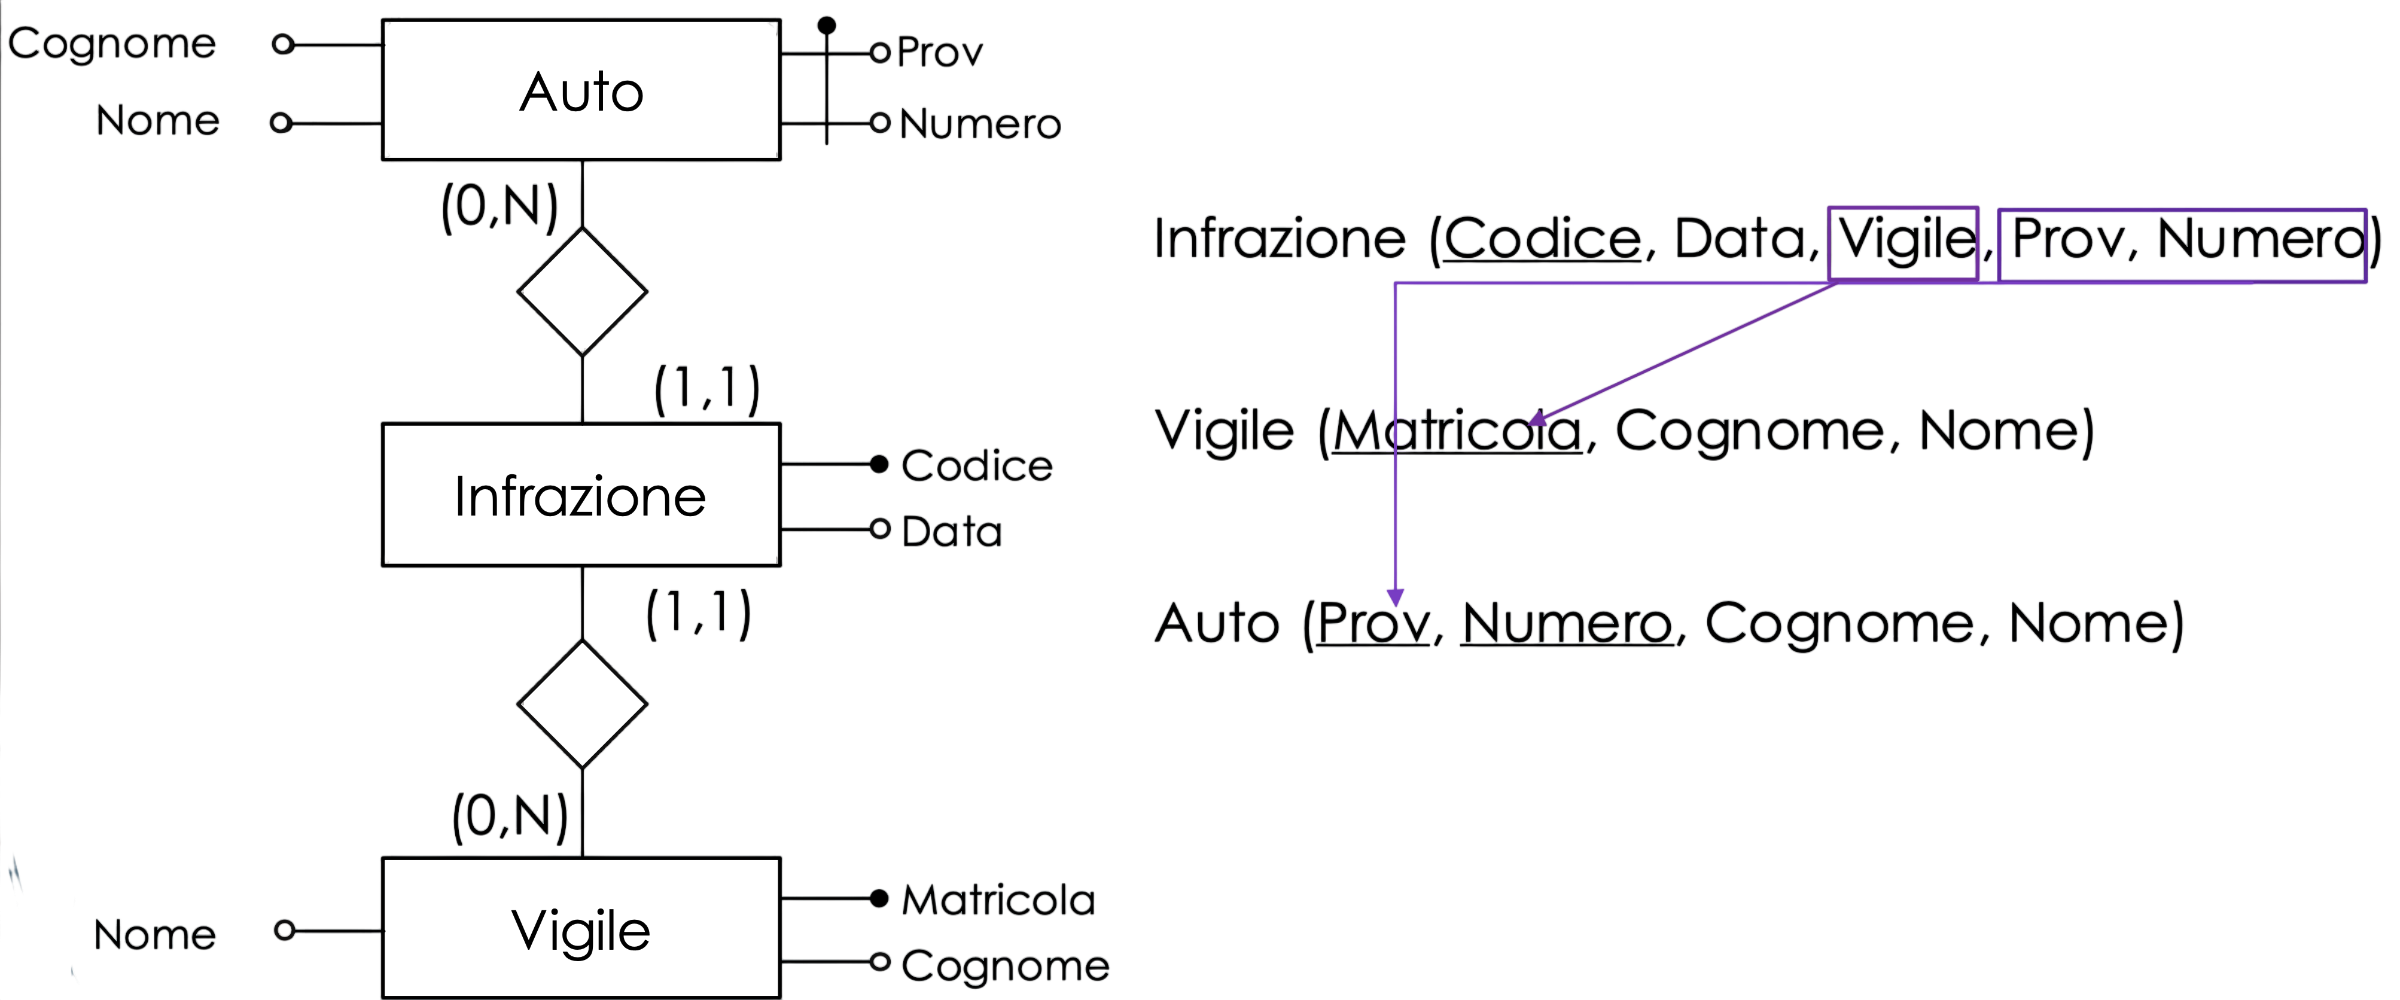
\includegraphics[width=0.7\textwidth]{images/esempioReferences.png}
\end{figure}

\begin{codiceSQL}
CREATE TABLE Infrazione(
  Codice CHAR(6) PRIMARY KEY, 
  Data DATE NOT NULL,  
  Vigile INTEGER NOT NULL
  REFERENCES Vigile(Matricola),
  Provincia CHAR(2),  
  Numero CHAR(6) ,
  FOREIGN KEY(Provincia, Numero)
    REFERENCES Auto(Provincia, Numero)
)
\end{codiceSQL}

\section{Modifica degli schemi}
\begin{itemize}[label=$\triangleright$, itemsep=\smallskipamount]
  \item \texttt{ALTER}: effettua modifiche (a domini, tabelle...), ad esempio aggiungere una colonna a una relazione
  \item \texttt{DROP DOMAIN}: permette di rimuovere i domini
  \item \texttt{DROP TABLE}: cancella una tabella
\end{itemize}

\subsection{Comando \texttt{ALTER TABLE}}
Il costrutto \texttt{ALTER} permette di:
\begin{itemize}[label=$\circ$, itemsep=\medskipamount]
  \item \textbf{aggiungere un nuovo attributo} (\texttt{ADD COLUMN}):
\begin{codiceSQL}
ALTER TABLE tabella
ADD COLUMN attributo tipo;

ALTER TABLE impiegato
ADD COLUMN stipendio NUMERIC(8,2);
\end{codiceSQL}
  \item \textbf{rimuovere un attributo} (\texttt{DROP COLUMN}):
\begin{codiceSQL}
ALTER TABLE tabella
DROP COLUMN attributo;

ALTER TABLE impiegato
DROP COLUMN stipendio;
\end{codiceSQL}
  \item \textbf{modificare valore di default di un attributo} (\texttt{ALTER COLUMN}):
\begin{codiceSQL}
ALTER TABLE tabella 
ALTER COLUMN attributo { SET DEFAULT valore | DROP DEFAULT };

ALTER TABLE impiegato 
ALTER COLUMN stipendio SET DEFAULT 1000.00;
\end{codiceSQL}
\end{itemize}

\section{Comando \texttt{DELETE} e \texttt{DROP TABLE}}
Le tuple di una tabella vengono cancellate con il comando \texttt{DELETE}:
\begin{codiceSQL}
DELETE FROM tabella [ WHERE condizione ];
\end{codiceSQL}

dove:
\begin{itemize}[label=$\triangleright$, itemsep=\smallskipamount]
  \item \texttt{condizione}: espressione booleana che seleziona quali tuple cancellare
\end{itemize}

\vario{Nota}{
  Se non viene specificata la condizione \texttt{WHERE}, verrano cancellate tutte le tuple.
}
\begin{codiceSQL}
DELETE FROM impiegato WHERE matricola = 'A001';
\end{codiceSQL}

\bigskip
Una tabella viene cancellata con il comando \texttt{DROP TABLE}:
\begin{codiceSQL}
  DROP TABLE tabella;
\end{codiceSQL}

\section{Comando \texttt{INSERT INTO} e \texttt{UPDATE}}
Il comando \texttt{INSERT INTO} permette di inserire valori all'interno di una tupla:
\begin{codiceSQL}
INSERT INTO Tabella [ ( Attributi ) ] 
VALUES( Valori )

--oppure

INSERT INTO Tabella [ ( Attributi )]
(SELECT ...)
\end{codiceSQL}

\begin{esempiobox}{Utilizzo di \texttt{INSERT INTO}}
\begin{codiceSQL}
INSERT INTO Museo(nome, citta, indirizzo, numeroTelefono, giornoChiusura, prezzo)
VALUES('Arena', 'Verona', 'piazza Bra', '045 8003204', 'MARTEDI', 20);
\end{codiceSQL}
\end{esempiobox}

\bigskip
Il comando \texttt{UPDATE} permette di aggiornare i valori all'interno di una tupla:
\begin{codiceSQL}
UPDATE NomeTabella
SET Attributo = < Espressione | SELECT ... | NULL | DEFAULT >
[ WHERE Condizione ]
\end{codiceSQL}

\begin{esempiobox}{Utilizzo di \texttt{INSERT INTO}}
\begin{codiceSQL}
UPDATE Museo SET sitoInternet = 'www.ciao.it' 
WHERE citta = 'Verona';  
\end{codiceSQL}
\end{esempiobox}


\section{Selezione}
La struttura base del comando di selezione è:
\begin{codiceSQL}
SELECT [ DISTINCT ]
[ * | expression [[ AS] output_name ] [, 
...] ]
FROM from_item [, ...] 
  [ WHERE condition ]
    [ GROUP BY grouping_element [, ...] ]
      [ HAVING condition [, ...] ]
      [ { UNION | INTERSECT | EXCEPT } [ DISTINCT
      ] other_select ]
        [ ORDER BY expression [ ASC | DESC | USING 
        operator ]]
\end{codiceSQL}


\subsection{Clausola \texttt{SELECT}}
\begin{codiceSQL}
SELECT [ DISTINCT ]
[{* | expression [[ AS] output_name ]} [, ...]]
\end{codiceSQL}

dove:
\begin{itemize}[label=$\triangleright$, itemsep=\smallskipamount]
  \item \texttt{*}: abbreviazione per indicare tutti gli attributi delle tabelle
  \item \texttt{expression}: espressione che coinvolge gli attributi della tabella (può anche essere semplicemente il nome di un attributo)
  \item \texttt{output\_name}: nome assegnato all’attributo che conterrà il risultato della valutazione dell’espressione expression nella relazione risultato.
  \item \texttt{DISTINCT}: se presente richiede l’eliminazione delle tuple duplicate
\end{itemize}

\smallskip
L’esecuzione di una \texttt{SELECT} produce una relazione che:
\begin{itemize}[label=$\circ$, itemsep=\smallskipamount]
  \item ha come schema tutti gli attributi elencati nella clausola \texttt{SELECT}
  \item ha come contenuto tutte le tuple ottenute proiettando sugli attributi indicati nella \texttt{SELECT} provenienti dalle tabelle del \texttt{FROM} (prodotto cartesiano), limitate a quelle che soddisfano le eventuali condizioni specificate nelle clausole \texttt{WHERE}, \texttt{GROUP BY} e \texttt{HAVING}
\end{itemize}

\subsubsection{Target List}

\begin{minipage}[t]{0.39\textwidth}
   \begin{codiceSQL}
SELECT *
FROM Tabella
   \end{codiceSQL}
\end{minipage}
\hfill % Questo comando inserisce uno spazio flessibile che spinge le due minipage ai lati opposti
\begin{minipage}[t]{0.50\textwidth}
  \vspace{1em}
   Selezione di tutti gli attributi 
delle tabelle indicate nella 
clausola FROM
\end{minipage}

\begin{minipage}[t]{0.39\textwidth}
   \begin{codiceSQL}
SELECT Attributo1, Attributo2
FROM Tabella
   \end{codiceSQL}
\end{minipage}
\hfill % Questo comando inserisce uno spazio flessibile che spinge le due minipage ai lati opposti
\begin{minipage}[t]{0.50\textwidth}
  \vspace{1em}
   Selezione di tutti gli attributi 
delle tabelle indicate nella 
clausola FROM
\end{minipage}

\begin{esempiobox}{Esempio}
\begin{codiceSQL}
SELECT Nome, Reddito
FROM Persone
  WHERE Eta < 30;
\end{codiceSQL}

  \begin{figure}[H]
    \centering
    \includegraphics[width=0.6\textwidth]{images/nomeReddito.png}
    \caption{selezione solo delle tuple dove è rispettata la condizione}
  \end{figure}
\end{esempiobox}


\subsubsection{Concatenazione stringhe}
L'operatore di concatenazione \texttt{||} è un operatore scalare (o operatore di riga).

Lavora su una singola riga alla volta.\\[0.2ex]
Se la tua tabella ha 100 righe, il costrutto \texttt{SELECT titolo || ' - ' || città} calcolerà e restituirà 100 risultati testuali separati, uno per ogni riga.

\vario{Nota}{
  Non è un'esclusiva di \texttt{SELECT}, può infatti essere utilizzato anche nella clausola \texttt{WHERE} e nella clausola \texttt{ORDER BY}.
}

\smallskip
La concatenazione all'interno della clausola \texttt{WHERE} serve per filtrare i dati:
\begin{codiceSQL}
WHERE nome || ' ' || cognome = 'Mario Rossi'
--Trova la riga in cui l'unione di nome e cognome da esattamente 
--'Mario Rossi'
\end{codiceSQL}

\smallskip
La concatenazione all'interno della clausola \texttt{ORDER BY} serve per ordinare i risultati:
\begin{codiceSQL}
ORDER BY titolo || citta
--Ordina i risultati basandosi sull'unione testuale dei due campi
\end{codiceSQL}


\subsection{Clausola FROM}
\begin{codiceSQL}
FROM from_item [, ...]
\end{codiceSQL}

dove:
\begin{enumerate}[itemsep=\smallskipamount]
  \item  \texttt{table\_name [[AS] alias [(column\_alias [, ...])]]}
  \begin{itemize}[itemsep=\smallskipamount]
    \item se sono presenti due o più tabelle, si esegue il prodotto cartesiano tra tutte le  tabelle
    \item se ci sono attributi con lo stesso nome su tabelle diverse, nel \texttt{SELECT} questi attributi sono identificati anteponendo il nome della tabella e un \texttt{’.’}:  \texttt{nomeTabella.nomeAttributo}
  \end{itemize}

  \item  (other\_select) [AS] nomeRisultato [(column\_alias [,...])
  \begin{itemize}
    \item  è una SELECT innestata. Il risultato della SELECT interna è lo schema con nome 
nomeRisultato su cui fare la SELECT corrente.
  \end{itemize}

  \item  from\_item [NATURAL] join\_type from\_item [ON condition]
  \begin{itemize}
    \item  è la clausola JOIN.
    \item Metodo più sofisticato di 1) che permette di selezionare un sottoinsieme del 
prodotto cartesiano di due o più tabelle. join\_type specifica il tipo di join. I tipi 
principali sono riassunti nelle slide seguenti
  \end{itemize}
\end{enumerate}


\subsubsection{Uso di alias}

\begin{codiceSQL}
SELECT P.Reddito, R.Telefono
FROM Reparti as R, Persona ad P
WHERE ... ;
\end{codiceSQL}

Utile quando è necessario specificare la provenienza dell’attributo, 
perchè nella base di dati sono presenti più attributi con lo stesso nome

\subsubsection{Target List}
\begin{codiceSQL}
SELECT P.Nome as NPersona, P.Reddito as RPersona
FROM Persone as P
WHERE P.Eta < 30
\end{codiceSQL}




\subsection{Clausola WHERE}
\begin{codiceSQL}
  WHERE condition
\end{codiceSQL}

\textbf{\textcolor{black!50!red}{condition}} è un’espressione booleana combinando condizioni semplici $C_{i}$ con gli 
operatori AND, OR, NOT.
\begin{enumerate}
  \item  $C_{i}$ := expr [ $\theta$ \{expr | const\}]
dove
\begin{itemize}
  \item expr := espressione che contiene riferimenti agli attributi delle tabelle che compaiono 
nella clausola FROM.
\item $\theta \in$ \{=,<>,<,>,<=,>=\}
\item const := valore dei domini di base.
\end{itemize}
\item Una riga soddisfa \textcolor{black!50!red}{condition} se l’espressione è vera quando valutata con i valori 
della riga.
\item Una riga che non soddisfa condition è scartata dal risultato finale
\end{enumerate}





\begin{minipage}[t]{0.39\textwidth}
 \begin{codiceSQL}
SELECT Nome, Reddito
FROM Persone
WHERE Eta < 30;
\end{codiceSQL}
\end{minipage}
\hfill % Questo comando inserisce uno spazio flessibile che spinge le due minipage ai lati opposti
\begin{minipage}[t]{0.50\textwidth}
SELECT Nome, Reddito
FROM Persone
WHERE Età < 30 OR Reddito > 50;
\end{minipage}




\subsubsection{Operatore LIKE}
\begin{codiceSQL}
WHERE attributo [NOT] LIKE 'pattern';
\end{codiceSQL}

Nella clausola WHERE può apparire l’operatore LIKE per il confronto di stringhe. 
LIKE è un operatore di pattern matching. I pattern si costruiscono con i 
caratteri speciali \_ e \%:
\begin{itemize}
  \item \_ = 1 carattere qualsiasi.
  \item \% = 0 o più caratteri qualsiasi.
\end{itemize}


\begin{minipage}[t]{0.39\textwidth}
  \vspace{2em}
  \begin{codiceSQL}
SELECT Nome,Reddito
FROM Persona
WHERE Nome LIKE 'A\%a'
  \end{codiceSQL}
\end{minipage}
\hfill 
\begin{minipage}[t]{0.50\textwidth}
  \vspace{0pt}
  % Rimosso totalmente \begin{figure}[H] e \end{figure}
  \includegraphics[width=0.8\textwidth]{images/nomeReddito2.png}
\end{minipage}  


\subsubsection{Operatore SIMILAR TO}


L’operatore \textbf{\textcolor{purple}{SIMILAR TO}} è un \textbf{\textcolor{purple}{LIKE}} più espressivo che accetta, come pattern, 
un sottoinsieme delle espressioni regolari POSIX (versione SQL). 
Esempi di componenti di espressioni regolari:
\begin{itemize}
  \item \_ = 1 carattere qualsiasi. 
  \item \% = 0 o più caratteri qualsiasi.
  \item * = ripetizione del precedente match 0 o più volte.
  \item + = ripetizione del precedente match UNA o più volte.
  \item \{n,m\} = ripetizione del precedente match almeno n e non più di m volte.
  \item {[} ... {]} = ... è un elenco di caratteri ammissibili
\end{itemize}


\begin{minipage}[t]{0.50\textwidth}
  \vspace*{0pt}
  \begin{codiceSQL}[unbreakable]
SELECT *
FROM Persone
WHERE Nome SIMILAR TO '[AFO]'
  \end{codiceSQL}
\end{minipage}
\hfill 
\begin{minipage}[t]{0.45\textwidth}
  \vspace*{0pt}
  \vspace{1.5em} % Spazio per allineare il testo al centro del codice
Per trovare nomi che inziano per A,F o O
\end{minipage}  


\subsubsection{Operatore BETWEEN}

\begin{codiceSQL}
WHERE attributo [NOT] BETWEEN valore_iniziale AND valore_finale;
\end{codiceSQL}

Nella clausola \textcolor{purple}{\textbf{WHERE}} può apparire l’operatore \textcolor{purple}{\textbf{BETWEEN}} per testare l’appartenenza 
di un valore ad un intervallo (non limitato ai valori numerici, usato anche con date e 
stringhe)


\begin{minipage}[t]{0.40\textwidth}
  \begin{codiceSQL} 
SELECT *
FROM Persone
WHERE Eta BETWEEN 20 AND 40
  \end{codiceSQL}
\end{minipage}
\hfill 
\begin{minipage}[t]{0.45\textwidth}
  \includegraphics[width=0.8\textwidth, valign=t]{images/nomeEtaReddito.png}
\end{minipage}


\subsubsection{Operatore IN}
\begin{codiceSQL}
  WHERE attributo [NOT] IN ( valore [, ...] );

\end{codiceSQL}
Nella clausola WHERE può apparire l’operatore [\textbf{\textcolor{purple}{NOT}}] \textbf{\textcolor{purple}{IN}} per testare 
l’appartenenza di un valore ad un insieme.
\begin{codiceSQL}
SELECT *
FROM Persone
WHERE Nome NOT IN ('Andrea', 'Franco')
\end{codiceSQL}

\subsubsection{Operatore IS NULL}
\begin{codiceSQL}
WHERE attributo IS [ NOT ] NULL;
\end{codiceSQL}
Nella clausola WHERE può apparire l’operatore \textbf{\textcolor{purple}{IS}} [\textbf{\textcolor{purple}{NOT}}] \textbf{\textcolor{purple}{NULL}} per testare se un 
valore è \textbf{\textcolor{purple}{NOT KNOWN (NULL)}} o no.
Il valore NULL non rappresenta lo zero o una stringa vuota, ma l'assenza di dati 
o un valore sconosciuto.
A partire dalle versioni SQL-2 è stata adottata una logica a tre valori (true, 
false, unknown) e i valori nulli non sono considerati né veri, né falsi.\par
\begin{center}
NON SI PUÒ usare ’=’ o ’<>’ con il valore NULL!  
\end{center}

\begin{codiceSQL}
SELECT *
FROM Persone
WHERE Reddito IS NOT NULL
\end{codiceSQL}

\subsubsection{Operatore ORDER BY}
\begin{codiceSQL}
  ORDER BY attributo [{ ASC | DESC }] [, ... ];
\end{codiceSQL}
La clausola ORDER BY ordina le tuple del risultato in ordine rispetto agli attributi 
specificati,
ASCendente è lo standard.
\begin{codiceSQL}
SELECT Nome
FROM Persone
ORDER BY Nome DESC

\end{codiceSQL}

\subsubsection{Operatori di aggregazione}


Sono operatori che permettono di determinare un valore considerando i valori 
ottenuti da una SELECT.
Due tipi principali:
\begin{itemize}
  \item COUNT.
  \item MAX, MIN, AVG, SUM.
\end{itemize}

\begin{codiceSQL}
SELECT MAX(Reddito) 
FROM Persone;
\end{codiceSQL}

\vario{Nota}{Quando si usano gli operatori aggregati, dopo la SELECT non possono 
comparire espressioni che usano i valori presenti nelle singole tuple perché il 
risultato è sempre e solo una tupla
}



  \begin{enumerate}
    \item \textbf{Count}
    \begin{codiceSQL}
      COUNT({ *| expr | ALLexpr | DISTINCTexpr }])
    \end{codiceSQL}
    Restituisce il numero di tuple significative nel risultato dell’interrogazione.
    Tre casi comuni:\begin{itemize}
      \item \textcolor{purple}{COUNT(*)} ritorna il numero di tuple nel risultato dell’interrogazione.
      \item \textcolor{purple}{COUNT(expr)} ritorna il numero di tuple in ciascuna delle quali il valore expr è non nullo
      \item \textcolor{purple}{COUNT(ALL expr)} include duplicati e valori nulli.
      \item \textcolor{purple}{COUNT(DISTINCT expr)} come con \textcolor{purple}{COUNT(expr)} ma con l’ulteriore condizione che i valori di expr siano distinti
    \end{itemize}
    \item \textbf{SUM/MAX/MIN/AVG} 
    \begin{codiceSQL}
      op ({ expr | DISTINCTexpr })
    \end{codiceSQL}
    Determinano un valore numerico (SUM/AVG) o alfanumerico (MAX/MIN) considerando le tuple significative nel risultato dell’interrogazione.
    \begin{itemize}
      \item op = SUM | AVG | MAX | MIN;
      \item expr è un’espressione che usa uno o più attributi e funzioni di attributi.
      \item DISTINCT considero solo i valori distinti.  
    \end{itemize}
    \begin{codiceSQL}
      SELECT AVG(Eta) AS Media\_Eta
      FROM Persone;
    \end{codiceSQL}
  \end{enumerate}


  \section{Esempi di interrogazioni}
  \subsection{Interrogazione con raggruppamento: Group by}

  Un raggruppamento è un insieme di tuple che hanno medesimi valori su uno o più attributi caratteristici del raggruppamento.\par
La clausola GROUP BY attr [, ...] permette di determinare tutti i raggruppamenti delle tuple della relazione risultato (tuple selezionate con la clausola WHERE) in funzione degli attributi dati.\par
In una interrogazione che usa GROUP BY, la clausola SELECT contiene solamente gli attributi (da 0 a tutti) utilizzati per il raggruppamento ed eventuali funzioni di aggregazione sugli altri attributi.


\textbf{\large Visualizzare tutte le città raggruppate della tabella Studente}
\begin{codiceSQL}
SELECT citta
FROM studente
GROUP BY citta
\end{codiceSQL}

\noindent
\begin{minipage}[t]{0.6\textwidth}
   \centering
   \includegraphics[width = 0.8\textwidth]{images/TableALL.png} 
\end{minipage}
\hfill % Questo comando inserisce uno spazio flessibile che spinge le due minipage ai lati opposti
\begin{minipage}[t]{0.38\textwidth}
   \centering
   \includegraphics[width = 0.4\textwidth]{images/Group_By.png} 
\end{minipage}




\textbf{\large Visualizzare tutte le città e i cognomi raggruppati}




\noindent
\begin{minipage}{0.5\textwidth}
   \begin{codiceSQL}
SELECT cognome,LOWER(citta)
FROM Studente
GROUP BY cognome,LOWER(citta);
   \end{codiceSQL}
\end{minipage}
\hfill % Questo comando inserisce uno spazio flessibile che spinge le due minipage ai lati opposti
\begin{minipage}[t]{0.40\textwidth}
   \centering
   \includegraphics[width = 0.5\textwidth]{images/tabellaRisultante.png} 
\end{minipage}




\vario{Nota}{Nel GROUP BY non si possono usare espressioni con operatori di aggregazione.}

\vario{Nota}{Nella SELECT con GROUP BY non si possono specificare attributi che non sono raggruppati.}



\begin{itemize}
  \item La clausola WHERE permette di selezionare le righe che devono far parte del risultato.
  \item La clausola HAVING permette di selezionare i raggruppamenti che devono far parte del risultato.
  \item La sintassi è HAVING bool\_expr, dove bool\_expr è un’espressione booleana che può usare gli attributi usati nel GROUP BY e/o gli altri attributi mediante operatori di aggregazione.
\end{itemize}


\textbf{\large Visualizzare tutte le città raggruppate che iniziano con ’V’ della tabella Studente.}



\noindent
\begin{minipage}{0.5\textwidth}
   \begin{codiceSQL}
SELECT citta
FROM Studente
GROUP BY citta
HAVING citta LIKE 'V%';
   \end{codiceSQL}
\end{minipage}
\hfill % Questo comando inserisce uno spazio flessibile che spinge le due minipage ai lati opposti
\begin{minipage}[t]{0.40\textwidth}
   \centering
   \includegraphics[width = 0.5\textwidth]{images/tabellaRisultante2.png} 
\end{minipage}




\textbf{\large Visualizzare tutte le città e i cognomi raggruppati con almeno due studenti con lo stesso cognome..}



\noindent
\begin{minipage}{0.5\textwidth}
   \begin{codiceSQL}
SELECT cognome, LOWER(citta)
FROM Studente
GROUP BY cognome, LOWER(citta)
HAVING COUNT ( cognome) >1;
   \end{codiceSQL}
\end{minipage}
\hfill % Questo comando inserisce uno spazio flessibile che spinge le due minipage ai lati opposti
\begin{minipage}[t]{0.40\textwidth}
   \centering
   \includegraphics[width = 0.5\textwidth]{images/tabellaRisultante3.png} 
\end{minipage}



\textbf{\large Si possono specificare espressioni con operatori di aggregazione su attributi non raggruppati anche nella clausola HAVING.}



\noindent
\begin{minipage}{0.5\textwidth}
   \begin{codiceSQL}
SELECT LOWER(citta) AS "Citta", AVG (media)::DECIMAL(5 ,2) AS "mediaArr."
FROM Studente
GROUP BY LOWER(citta)
HAVING AVG(media) >23.47 ;
   \end{codiceSQL}
\end{minipage}
\hfill % Questo comando inserisce uno spazio flessibile che spinge le due minipage ai lati opposti
\begin{minipage}[t]{0.40\textwidth}
   \centering
   \includegraphics[width = 0.5\textwidth]{images/tabellaRisultante4.png} 
\end{minipage}



\subsection{Interrogazione con JOIN}

\begin{codiceSQL}
  TABLE1 join_type TABLE2 ON join_condition[, ...].
\end{codiceSQL}


\textcolor{cyan}{INNER JOIN}, \textcolor{cyan}{LEFT [OUTER] JOIN}, \textcolor{cyan}{RIGHT [OUTER] JOIN} e \textcolor{cyan}{FULL [OUTER] JOIN}.
Dove \textcolor{cyan}{join\_condition} è un’espressione booleana che seleziona le tuple del join da aggiungere al risultato.
Le tuple selezionate possono essere poi filtrate con la condizione della clausola \textcolor{purple}{WHERE}.
Il prodotto cartesiano di due o più tabelle è un \textcolor{cyan}{CROSS JOIN}.


\textbf{\large Interrogazioni con INNER JOIN}

\begin{codiceSQL}
  table1 [INNER] JOIN table2 ON join_condition[, ...]
\end{codiceSQL}


Rappresenta il tradizionale $\theta$ join dell’algebra relazionale.
Combina ciascuna riga \texttt{r1} di \texttt{table1} con ciascuna riga di \texttt{table2} che soddisfa la condizione della clausola ON.



\subsection{Interrogazioni con LEFT OUTER JOIN}
\begin{codiceSQL}
  table1 LEFT[OUTER] JOIN table2 ON join_condition[, ...].
\end{codiceSQL}

Si esegue un INNER JOIN. Poi, per ciascuna riga \texttt{r1} di \texttt{table1} che non soddisfa la condizione con qualsiasi riga di \texttt{table2}, si aggiunge una riga al risultato con i valori di \texttt{r1} e assegnando NULL agli altri attributi..

Il LEFT [OUTER] JOIN non è simmetrico!
Con le medisime tabelle si possono ottenere risultati diversi invertendo l’ordine delle tabelle nel join!


\subsection{Interrogazioni con RIGHT OUTER JOIN}

\begin{codiceSQL}
  table1 RIGHT[OUTER] JOIN table2 ON join_condition[, ...].
\end{codiceSQL}

Si esegue un INNER JOIN. Poi, per ciascuna riga r2 di table2 che non soddisfa la condizione con qualsiasi riga di table1, si aggiunge una riga al risultato con i valori di r2 e assegnando NULL agli altri attributi..


\subsection{Interrogazioni con FULL OUTER JOIN}

\begin{codiceSQL}
  table1 FULL[OUTER] JOIN table2 ON join\_condition[, ...].
\end{codiceSQL}

\begin{itemize}
  \item È equivalente a: INNER JOIN + LEFT OUTER JOIN + RIGHT OUTER JOIN.
  \item \textcolor{black!60!red}{Non è equivalente a CROSS JOIN!}
\end{itemize}


\vario{Quando usare left join rispetto a right join?}{
\begin{itemize}
  \item \textbf{JOIN}: Solo i record che fanno "match" in entrambe le tabelle.
  \item \textbf{LEFT JOIN}:	Tutto ciò che sta nella prima tabella scritta, con i NULL se manca il pezzo della seconda.
  \item \textbf{RIGHT JOIN}: Tutto ciò che sta nella seconda tabella scritta, con i NULL se manca il pezzo della prima.
  \item \textbf{FULL JOIN}: Tutti i dati di entrambe le tabelle, allineando ciò che combacia e mettendo NULL ovunque manchi una corrispondenza.
\end{itemize}
}

  \section{Interrogazioni nidificate e insiemistiche}

  \subsection*{Interrogazioni nidificate}
  SQL permette la costruzione di interrogazioni che presentano al loro interno altre interrogazioni. 
La nidificazione può avvenire nelle clausole \textcolor{purple}{SELECT}, \textcolor{purple}{FROM}, \textcolor{purple}{WHERE}.

\underline{L'uso più comune è la nidificazione nella clausola WHERE}

\subsection{Clausola FROM}
Con l'utilizzo di questa opzione, è possibile comporre catene di interrogazioni, 
in cui ciascuna interrogazione utilizza il risultato della precedente come se 
fosse una tabella di base

\begin{codiceSQL}
  SELECT titolo, prezzoIntero
FROM Mostra, ( 
  SELECT MAX ( prezzoIntero ) 
  FROM Mostra 
) AS T( prezzoMax )
WHERE prezzoIntero = prezzoMax;
\end{codiceSQL}
dove:
\begin{itemize}
  \item \textbf{T}: alias della tabella. La query interna ha generato una tabellina "anonima", noi la chiamiamo temporaneamente con la lettera T
  \item \textbf{(prezzoMax)}: alias della colonna
\end{itemize}


\subsection{Clausola WHERE}
Il predicato (predicato complesso) nella clausola WHERE confronta un valore (ottenuto come espressione valutata sulla singola riga), con il risultato dell'esecuzione di un'interrogazione SQL (in generale un insieme di valori). 
Occorre estendere gli operatori di confronto per poter realizzare la comparazione tra un valore e un insieme di valori



Soluzione offerta da SQL: estensione degli operatori di confronto (>,<, =, <=, 
>=, <>) con ANY/SOME e ALL (IN, NOT IN). 
\begin{itemize}
  \item \textcolor{purple}{ANY/SOME}: specifica che la riga soddisfa la condizione se risulta vero il 
confronto (con l'operatore specificato) tra il valore dell'attributo per la riga e 
\textbf{almeno uno} degli elementi restituiti dall'interrogazione. 
  \item \textcolor{purple}{ALL}: specifica che la riga soddisfa la condizione solo se \textbf{tutti gli elementi} 
restituiti dall'interrogazione nidificata rendono vero il confronto. 
\item \textcolor{purple}{IN} e \textcolor{purple}{NOT IN}: usati per rappresentare l'appartenenza o l'esclusione rispetto ad 
un insieme (identici a = ANY o <>ALL)
\end{itemize}


\subsubsection{Operatore ANY/SOME}
\begin{codiceSQL}
  expression operator ANY( subquery )
expression operator SOME( subquery )
\end{codiceSQL}

\begin{itemize}
  \item \textcolor{orange}{expression} è un’espressione che coinvolge attributi della SELECT principale.
  \item (\textcolor{orange}{subquery}) è una \textcolor{purple}{SELECT} che deve restituire UNA sola colonna;
  \item \textcolor{orange}{operator} è un operatore di confronto, come ’=’, ’>=’, ...
  \item \textcolor{purple}{ANY}: è vero se la condizione è vera per almeno un valore della subquery.
  \item \textcolor{purple}{SOME} è uno sinonimo di \textcolor{purple}{ANY}
\end{itemize}


\textbf{\large Visualizzare il nome degli insegnamenti che hanno un numero di crediti 
inferiore alla media dell’ateneo di un qualsiasi anno accademico.}

\begin{codiceSQL}
  SELECT DISTINCT I.nomeins , IE.crediti
FROM Insegn I 
  JOIN InsErogato IE ON I.id=IE.id_insegn
WHERE IE.crediti < ANY (
  SELECT AVG ( crediti ) 
  FROM InsErogato
  WHERE modulo =0
  GROUP BY annoaccademico
  );
\end{codiceSQL}


\subsubsection{Operatore ALL}
\begin{codiceSQL}
  expression operator ALL( subquery )
\end{codiceSQL}

\begin{itemize}
  \item  \textcolor{orange}{expression} è un’espressione che coinvolge attributi della SELECT principale.
  \item (\textcolor{orange}{subquery}) è una \textcolor{purple}{SELECT} che deve restituire UNA sola colonna;
  \item \textcolor{orange}{operator} è un operatore di confronto, come ’=’, ’>=’, ...
  \item \textcolor{purple}{ALL}: La condizione è vera solo se è vera per TUTTI i valori della subquery.

\end{itemize}

\textbf{\large Trovare il nome degli insegnamenti con almeno un docente e crediti maggiori rispetto ai 
crediti di ciascun insegnamento del corso di laurea con id=6. (si considerano solo 
occorrenze insegnamento genitore)}

\begin{codiceSQL}
  SELECT DISTINCT I. nomeins , IE. crediti
FROM Insegn I 
  JOIN InsErogato IE ON I.id = IE. id_insegn
  JOIN Docenza D ON IE.id = D. id_inserogato
WHERE IE. modulo = 0 AND IE. crediti > ALL (
  SELECT crediti 
  FROM InsErogato
  WHERE id_corsostudi = 6 AND modulo =0
  );
\end{codiceSQL}

\subsubsection{Operatore IN}
E’ un operatore utilizzabile nei predicati complessi.
\begin{codiceSQL}
ROW ( expr [ ,...]) IN ( subquery )  
\end{codiceSQL}
\begin{itemize}
  \item \textcolor{orange}{expr} è un’espressione costruita con un attributo della query principale. Ci 
possono essere una o più espressioni.
\item La (\textcolor{orange}{subquery}) deve restituire un numero di colonne pari al numero di 
espressioni in (\textcolor{orange}{expr} [,...]).
\item I valori dell’espressioni vengono confrontati con i valori di ciascuna riga del 
risultato di (subquery).
\item Il confronto ritorna vero se i valori sono uguali ai valori di almeno una riga della 
subquery.
\end{itemize}



\textbf{\large Trovare gli impiegati che hanno stesso nome e cognome di qualcuno in 
un’altra azienda.}
\begin{codiceSQL}
SELECT I.nome , I.cognome
FROM Impiegato I
WHERE ROW( I.nome , I.cognome ) IN (
SELECT I1.nome, I1.cognome FROM ImpiegatoAltraAzienda I1)
\end{codiceSQL}



\subsubsection{Operatore EXIST}
E’ una clausola utilizzabile nei predicati complessi
\begin{codiceSQL}
  EXISTS(subquery)
\end{codiceSQL}


\begin{itemize}
  \item (subquery) è una \textcolor{purple}{SELECT}.
  \item \textcolor{purple}{EXISTS} ritorna falso se (subquery) non contiene righe; altrimenti vero.
  \item \textcolor{purple}{EXISTS} è significativo quando nella (subquery) si selezionano righe usando i 
valori della riga corrente nella \textcolor{purple}{SELECT} principale: \textcolor{black!60!red}{data binding. 
Vale a dire se subquery è un'interrogazione dipendente dalla query esterna}
\end{itemize}


\textbf{\large Determinare i nomi degli impiegati che sono diversi tra loro ma di pari 
lunghezza}

\begin{codiceSQL}
  SELECT I. nome
FROM Impiegato I
WHERE EXISTS (
  SELECT 1 
  FROM Impiegato I1 
  WHERE I.nome <> I1. nome AND CHAR_LENGTH( I.nome ) = CHAR_LENGTH( I1. nome )
)
\end{codiceSQL}
\texttt{I.nome} nella subquery è il valore di nome nella riga corrente della SELECT 
principale


\vario{Nota }{Se si usano attributi esterni nella subquery (data binding), la subquery
deve essere valutata per ogni riga della SELECT principale}


\textbf{\large Visualizzare il nome e il cognome dei docenti, escludendo i coordinatori, che hanno 
tenuto almeno due insegnamenti (o moduli) con più di 24 crediti nel 2010/2011}

\begin{codiceSQL}
  SELECT P.nome , P.cognome
FROM Persona P
WHERE EXISTS (
SELECT 1 
FROM Docenza D 
  JOIN InsErogato IE ON D. id_inserogato = IE.id
WHERE IE. crediti > 24 AND D. coordinatore = '0'
AND IE. annoaccademico = '2010/2011' AND D. id_persona = P.id
GROUP BY D. id_persona
HAVING COUNT (*) >=2
);

\end{codiceSQL}

\textbf{\large Visualizzare il nome dei corsi di studio che nel 2006/2007 non
hanno 
erogato insegnamenti il cui nome contiene la sottostringa ’Info’.}


\begin{codiceSQL}
  SELECT CS. nome FROM CorsoStudi CS
WHERE NOT EXISTS (
  SELECT 1 
  FROM InsErogato IE 
    JOIN Insegn I ON IE. id_insegn = I.id
  WHERE I.nomeins LIKE '%Info%'
  AND IE.annoaccademico = '2006/2007'
  AND IE.id_corsostudi = CS.id
)
\end{codiceSQL}



\subsection*{Interrogazioni di tipo insiemistico}

\begin{codiceSQL}
  query_1 { UNION | INTERSECT | EXCEPT } [ALL] query_2
\end{codiceSQL}

SQL mette a disposizione anche degli operatori insiemistici \texttt{UNION}, \texttt{INTERSECT} e 
\texttt{EXCEPT} per manipolare i risultati di più query.
Gli operatori insiemistici si possono utilizzare solo al livello più esterno di una 
query, operando sul risultato di due o più clausole \texttt{SELECT}.
Si possono avere sequenze di \texttt{UNION/INTERSECT/EXCEPT}


Gli operatori si possono applicare solo quando \textcolor{cyan}{query1} e \textcolor{cyan}{query2} producono 
risultati con lo stesso numero di colonne e di tipo compatibile fra loro.
Tutti gli operatori eliminano i duplicati dal risultato a meno che ALL non sia 
stato specificato.
\begin{itemize}
  \item \textcolor{red}{\textbf{UNION}} aggiunge il risultato di \textcolor{cyan}{query2} a quello di \textcolor{cyan}{query1}.
  \item \textcolor{red}{\textbf{INTERSECT}} restituisce le righe che sono presenti sia nel risultato di \textcolor{cyan}{query1} sia in quello di \textcolor{cyan}{query2}
  \item \textcolor{red}{\textbf{EXCEPT}} restituisce le righe di \textcolor{cyan}{query1} che non sono presenti nel risultato di \textcolor{cyan}{query2}. In pratica esegue la differenza insiemistica


\end{itemize}


\textbf{\large Visualizzare i nomi degli insegnamenti e i nomi dei corsi di laurea 
che non iniziano per 'A' mantenendo i duplicati}

\begin{codiceSQL}
  SELECT nomeins
FROM Insegn
WHERE NOT nomeins LIKE 'A%'
UNION ALL
SELECT nome
FROM CorsoStudi
WHERE NOT nome LIKE 'A%'
\end{codiceSQL}

    
\textbf{\large
  Visualizzare i nomi degli insegnamenti che sono anche nomi 
di corsi di laurea.
}

\begin{codiceSQL}
  SELECT nomeins
FROM Insegn
INTERSECT ALL
SELECT nome
FROM CorsoStudi;
\end{codiceSQL}

\textbf{\large Visualizzare i nomi degli insegnamenti che NON sono anche 
nomi di corsi di laurea.}

\begin{codiceSQL}
  SELECT nomeins
FROM Insegn
EXCEPT
SELECT nome
FROM CorsoStudi;
\end{codiceSQL}

\subsection{Le viste}

Le viste sono tabelle virtuali il cui contenuto dipende dal contenuto delle altre 
tabelle della base di dati.
In SQL le viste vengono definite associando un nome ed una lista di attributi al 
risultato dell’esecuzione di un’interrogazione.
\textcolor{purple}{Ogni volta che si usa una vista, si esegue la query che la definisce.}
Nell’interrogazione che definisce la vista possono comparire anche altre viste.
SQL \textcolor{red}{non ammette} però
\begin{itemize}
  \item  dipendenze immediate (definire una vista in termini di se stessa) o ricorsive 
(definire una interrogazione di base e una interrogazione ricorsiva);
\item dipendenze transitive circolari (V1 definita usando V2, V2 usando V3,. . . , Vn
usando V1).
\end{itemize}

\begin{codiceSQL}
  CREATE [ TEMP ] VIEW nome [( col_name [, ...]) ] AS query

\end{codiceSQL}

\textcolor{purple}{TEMP}: la vista è temporanea. Quando ci si sconnette, la vista viene distrutta. È 
un’estensione di PostgreSQL. Nella base di dati did2014 si possono fare solo 
viste temporanee

\begin{itemize}
  \item  \textcolor{cyan}{column\_name}: nomi delle colonne che compongono la vista; se non 
vengono specificati, sono ricavati dai nomi delle colonne restituiti dalla 
query, eventualmente tramite alias.
\item \textcolor{cyan}{query} deve restituire un insieme di attributi pari e nel medesimo ordine a 
quello specificato con ( \textcolor{cyan}{column\_name} [, ...] ) se presente.
\item SQL permette che una vista sia aggiornabile solo quando ciascuna tupla
della vista corrisponde a una sola tupla di ciascuna tabella di base.

\end{itemize}


\textbf{\large Definire la vista che contiene gli insegnamenti erogati completi di nomeins e codiceins
presi dalla tabella Insegn.}

\begin{codiceSQL}
  CREATE TEMP VIEW InsErogatiCompleti AS
SELECT I. nomeins , I. codiceins , IE .*
FROM InsErogato IE
JOIN Insegn I ON IE. id_insegn = I.id;
\end{codiceSQL}


\textbf{\large Si vuole determinare quali sono i corsi di studi con il massimo numero di nome di insegnamenti 
diversi}

Prima si crea una vista:

\begin{codiceSQL}
  CREATE TEMP VIEW InsCorsoStudi (Nome , NumIns) AS
SELECT CS.nome , COUNT ( DISTINCT I. nomeins )
FROM CorsoStudi CS
JOIN InsErogato IE ON CS.id=IE. id_corsostudi
JOIN Insegn I ON IE. id_insegn = I.id 
GROUP BY CS.nome;

\end{codiceSQL}

Poi la si usa:

\begin{codiceSQL}
  SELECT Nome, NumIns
FROM InsCorsoStudi
WHERE NumIns = ANY (
SELECT MAX ( NumIns ) FROM InsCorsoStudi);
\end{codiceSQL}

Laurea specialistica in Medicina e Chirurgia: 320

\section{Indici}

Gli indici sono delle \textbf{strutture dati ausiliare} che permettono di accedere ai dati di una tabella in maniera più efficiente.
Essendo una struttura dati ausiliaria, deve essere sempre mantenuta aggiornata in base al contenuto della tabella in cui è definita.
Il costo di aggiornamento può essere significativo quando ci sono molti indici definiti sulla medesima tabella.
\underline{Gli indici quindi devono essere definiti considerando la loro utilità.}

Si consideri il seguente schema fisico
\begin{codiceSQL}
InsErogato(id, id_insegn, id_corsostudi, id_discriminante, annoaccademico, id_facolta, modulo, nomemodulo, discriminantemodulo, crediti, programma)
Insegn(id, nomeins, codiceins)
Discriminante(id, nome, descrizione)
CorsoStudi(id, nomecorsostudi, sede, durataAnni)
CorsoInFacolta(id, id_corsostudi, id_facolta)
Facolta(id, nome)
\end{codiceSQL}

\subsection*{Query SENZA indici}
Si consideri la query:
\begin{codiceSQL}
SELECT id, nomeins FROM Insegn WHERE nomeins='Algoritmi';  
\end{codiceSQL}
Il DBMS deve fare una scansione sequenziale della tabella Insegn rispetto nomeins per estrarre le righe con valore uguale a 'Algoritmi';


Il comando \texttt{\textbackslash timing} attiva/disattiva la visualizzazione del tempo di pianificazione + calcolo di una query.
Il tempo è visualizzato subito dopo la visualizzazione del risultato della query.
\texttt{\textbackslash timing} dà un’idea del tempo necessario per eseguire una query.



\begin{codiceSQL}
=>\timing
Timing is ON.
=> SELECTid , nomeins
FROM Insegn
WHERE nomeins='Algoritmi';


id | nomeins
-----+--------------
5441 | Algoritmi

(1 row)
TIME: 2.437 ms
\end{codiceSQL}

Il tempo è di 2 millisecondi circa

\subsection{Creazione indice}
\begin{codiceSQL}
  CREATE INDEX[ nome]ON nomeTabella[ USING method ]
({ nomeAttr|( expression )} [ASC| DESC] [, ...])
CREATE INDEX Nome Indice ON NomeTabella (ListaAttributi)
\end{codiceSQL}

\begin{itemize}
  \item \textcolor{cyan}{\textbf{method}} è il tipo di indice;
  \item \textcolor{cyan}{\textbf{nomeAttr}} o \textcolor{cyan}{ \textbf{expression}} indicano su quali espressione di attributi si deve creare indice.
  \item \textcolor{purple}{\textbf{ASC/DESC}} specifica se l’indice è ordinato in modo ascendente o discendente.
  \item \textcolor{purple}{\textbf{ALTER INDEX}} e \textcolor{purple}{\textbf{DROP INDEX}} permettono di modificare/rimuovere indici creati precedentemente.
\end{itemize}

Un DBMS crea gli indici in modo automatico solo per attributi dichiarati PRIMARY KEY (\textcolor{purple}{\textbf{indice primario}}).

Per tutti gli altri attributi si deve fare una dichiarazione esplicita di \textcolor{purple}{\textbf{CREATE INDEX}}.

\begin{codiceSQL}
  ANALYZE nomeTabella;
\end{codiceSQL}

Il comando \texttt{ANALYZE[nomeTabella]} aggiorna le statistiche circa il contenuto delle tabelle (e indici). È eseguito in modo automatico dal sistema a intervalli regolari.
L’ottimizzatore di query usa queste statistiche per decidere quando usare gli indici.

\subsection*{Query CON indici}

Per rendere più veloce l’esecuzione della query:
\begin{codiceSQL}
SELECT id, nomeins FROM Insegn WHERE nomeins='Algoritmi';
\end{codiceSQL}
un indice sull’attributo nomeinspotrebbe essere utile perché nomeinsè l’attributo usato per selezionare le righe.
Query CON

\begin{codiceSQL}
  => CREATE INDEX nomeins_index ON Insegn( nomeins);
=> ANALYZE Insegn;
=> SELECT id, nomeins FROM Insegn WHERE nomeins='Algoritmi';

id | nomeins
-----+---------------
5441 | Algoritmi
TIME: 0.587 ms
\end{codiceSQL}
\textcolor{red}{\textbf{Il tempo di esecuzione è passato da 2.4337 msa 0.587 ms.}}

\vario{Nota}{Nota:Non è garantito che il tempo di esecuzione sia sempre uguale perché il server è multitask. I tempi di queste slide sono stati determinati con il server completamente dedicato}

\subsection{Caso pratico}

Si consideri la seguente query senza Indici

\begin{codiceSQL}
SELECT DISTINCT I.nomeins
FROM CorsoStudi CS
JOIN InsErogato IE ON CS.id = IE.id_corsostudi
JOIN Insegn I ON I.id = IE.id_insegn
WHERE IE.annoaccademico = '2009/2010'
AND CS.nome = 'Laurea in Informatica';
...
(26 ROWS )
TIME : 40.975 ms
\end{codiceSQL}
\textcolor{black!60!red}{\textbf{Quanto è possibile rendere più veloce la query definendo degli indici?}}

Una possibilità è definire gli indici su tutti gli attributi usati per fare i JOIN o le selezioni

\begin{codiceSQL}
CREATE INDEX cs_id ON CorsoStudi(id);
CREATE INDEX i_id ON Insegn(id);
\end{codiceSQL}

\vario{Nota}{Gli indici sugli attributi PRIMARY KEY (id nel nostro caso) solitamente sono già presenti! In did2014small sono stati tolti per fare gli esperimenti}

Si consideri la creazione degli indici:
\begin{codiceSQL}
CREATE INDEX ie_id_corsostudi ON Inserogato( id_corsostudi);
CREATE INDEX ie_id_insegn ON Inserogato( id_insegn);
CREATE INDEX ie_aa ON Inserogato( annoaccademico);
CREATE INDEX cs_nome ON Corsostudi( nome );
ANALYZE Corsostudi;
ANALYZE Inserogato;
ANALYZE Insegn;
\end{codiceSQL}

Non tutti gli indici sono necessari, ma per ora accettiamo il costo di crearli tutti.
Importante! Forziamo il DBMS ad aggiornare le statistiche con il comando ANALYZE dopo la creazione degli indici.


Con la creazione degli indici, la query richiede un tempo inferiore:
\begin{codiceSQL}
SELECT DISTINCT I.nomeins
FROM Corso StudiCS
JOIN InsErogato IE ON CS.id= IE.id_corsostudi
JOIN InsegnI ON I.id= IE.id_insegn
WHERE IE.annoaccademico= '2009/2010'
AND CS.nome= 'Laurea in Informatica';
...
(26 ROWS )
TIME : 5.201 ms
\end{codiceSQL}

Il tempo di esecuzione è passato da ~40 ms a ~5 ms.

\subsection{Tipi di indice}
PostgreSQL ammette diversi tipi di indici: B-tree, hash, GiST, SP-GiST, GIN e BRIN.
Sintassi per specificare anche il tipo:
\begin{codiceSQL}
CREATE INDEX nome ON nomeTab USING type(COLUMN);
\end{codiceSQL}

\subsubsection{B-tree}
Se nel CREATE INDEX non si specifica il tipo di indice, il sistema crea un indice di tipo B-tree.
L’ottimizzatore di query considera un indice B-tree ogni volta che l’attributo indicizzato è coinvolto in un confronto usando uno degli operatori: <, <=, =, >=, >.
Un indice B-tree può essere considerato anche quando ci sono \textcolor{purple}{\textbf{BETWEEN}}, \textcolor{purple}{\textbf{IN}}, \textcolor{purple}{\textbf{IS NULL}}, \textcolor{purple}{\textbf{IS NOT NULL}} e \textcolor{purple}{\textbf{LIKE}} 'abc\%'.


Con la localizzazione (it\_IT.UTF-8), la comparazione di stringhe con operatori diversi da ’=’ e con \textcolor{purple}{\textbf{LIKE}} ha regole diverse (minuscole/maiuscole) rispetto a UTF8.
Un indice su attributo VARCHAR in una base di dati con LC\_LOCALE = it\_IT.UTF-8 (come le basi di dati in dbserver) dovrebbe essere dichiarato come:
\begin{codiceSQL}
CREATE INDEX nome ON nomeTab(nomeAttrvarchar_pattern_ops);
\end{codiceSQL}
se si vuole che l'indice sia usato anche quando il confronto usa <,>,<>, LIKE.
La parola chiave \textcolor{purple}{\textbf{varchar\_pattern\_ops}} abilita l'uso degli operatori rispettando le regole imposte dal locale (it\_IT.UTF-8).

\subsubsection{Hash}

Il tipo \textbf{hash} ha un uso limitato perché può essere usato solo quando i confronti sonodi eguaglianza.
La sua gestione poi è più complicata in basi di dati replicate o in caso di crash: il gruppo di PostgreSQL ne sconsiglia l’uso.
Gli altri tipi di indici sono indicati per particolari strutture dati. Per esempio, GiST è indicato quando un attributo è di tipo geometrico bi-dimensionale(tipo non standard).

\subsubsection{Multi-attributo}
Se si hanno query che hanno condizioni su coppie (terne, ecc) di attributi di una tabella, un indice multi-attributo definito usando la coppia (terna, ecc) di attributi potrebbe essere più utile rispetto gli indici sui singoli attributi.

Creazione indice multi-attributo
\begin{codiceSQL}
CREATE INDEX ie_aa_idcs ON

Inserogato( annoaccademico, id_corsostudi);
ANALYZE Inserogato;

SELECT I.nomeins, I.codiceins
FROM InsegnI JOINInsErogatoIE ONI.id= IE. id_insegn
WHERE IE. annoaccademico= '2006/2007 '
ANDIE. id_corsostudi= 4;

...(46 ROWS )
TIME : 1.910 ms
\end{codiceSQL}



NON sempre gli indici multi-attributo possono essere usati: per esempio in espressioni con OR non è possibile.
\begin{codiceSQL}
SELECT I. nomeins, I. codiceins
FROM InsegnI JOIN InsErogatoIE ONI.id= IE. id_insegn
WHERE IE.annoaccademico= '2006/2007' OR IE.id_corsostudi= 4;
...(5334 ROWS )  
\end{codiceSQL}


\begin{itemize}
  \item Non c’è il tempo di esecuzione perché il risultato è diverso e quindi non comparabile.
  \item In questa query l’indice \textbf{ie\_aa\_idcs} NON è usato perché la disgiunzione \textcolor{purple}{OR} rende impossibile di fatto il suo uso.
  \item Nemmeno gli indici singoli ie\_id\_corsostudi e ie\_aa sono usati.
  \item L’ottimizzatore esegue una scansione di tutta la tabella Insegn.
\end{itemize}


\subsubsection{Indici di espressioni}
È possibile definire indici anche usando espressioni di attributi.
\begin{codiceSQL}
  CREATE INDEX nome ON nomeTabella(expression);
\end{codiceSQL}
dove expression è una espressione su uno o più attributi.


Query con indici definiti usando espressioni:
\begin{codiceSQL}
CREATE INDEX ins_lower_nonins ON Insegn
( LOWER( nomeins) varchar_pattern_ops);
ANALYZE Insegn;
SELECT nomeins FROM Insegn
WHERE LOWER(nomeins) LIKE 'algoritmi %';
...(4 ROWS )
TIME : 1.796 ms
  
\end{codiceSQL}

\subsection{Costo e Pratiche d'uso}
Gli indici costano tempo e memoria.
Se si considera solo il tempo, il costo maggiore è mantenere gli indici aggiornati.
Per ogni operazione di INSERT, UPDATE, DELETE su una tabella con indici, il DBMS deve aggiornare anche gli indici della tabella.

\textcolor{black!60!red}{Regola pratica: definire gli indici in base alle query più frequenti.}

Il comando PostgreSQL \texttt{\textbackslash di} visualizza l’elenco degli indici definiti in una base di dati.

Il comando PostgreSQL \texttt{\textbackslash d} nomeTabella visualizza la definizione di tabella e degli indici associati.


\subsubsection*{Perchè questo?}
Un DBMS ha un ottimizzatore di query che determina un piano per eseguire una data query nel minor tempo possibile.
Il comando \texttt{EXPLAIN} permette di vedere il piano di esecuzione di una query che l’ottimizzatore determina senza eseguire la query.
Un piano di esecuzione di una query è un albero di nodi di esecuzione.

Le foglie sono nodi di scansione: l’esecuzione di questi nodi restituiscono indirizzi di righe della tabella.

\subsubsection*{Struttura}

Esistono differenti tipi di scansioni: \textbf{sequenziali}, \textbf{indicizzate} e \textbf{mappate su bit}.
\begin{itemize}
  \item Se una query contiene \texttt{\textcolor{purple}{JOIN}}, \texttt{\textcolor{purple}{GROUP BY}} o \texttt{\textcolor{purple}{ORDER BY}} o altre operazioni sulle righe, \textcolor{purple}{allora ci saranno altri nodi di esecuzione sopra le foglie nell’albero}.
  \item L’output di \texttt{EXPLAIN} ha una riga per ciascun nodo nell’albero di esecuzione dove viene indicato il tipo di operazione e una stima del costo di esecuzione.
  \item Ulteriori proprietà del nodo possono essere mostrate con una riga indentata subito sotto.
  \item La prima riga dell’output ha la stima del costo totale di esecuzione della query. Questo è il costo che l’ottimizzatore cerca di minimizzare.
\end{itemize} 

\begin{codiceSQL}
EXPLAIN SELECT* FROM Insegn;
QUERY PLAN
------------------------------------------------------------
SeqScan ON insegn(cost=0.0..185.69 ROWS=8169 width=63)  
\end{codiceSQL}
\begin{itemize}
  \item 0.0 è il costo iniziale, per produrre la prima riga(in termini di numero di accessi alla memoria secondaria).
  \item 185.69 è il costo totale, per produrre tutte le righe.
  \item 8169 è il numero totale di righe del risultato(Il numero totale di righe non è sempre il numero totale di righe valutate dall’esecutore).
  \item 63 è la dimensione, in byte, di ciascuna riga.
\end{itemize}

\subsubsection{Explain con due nodi}
\begin{codiceSQL}
EXPLAIN SELECT* FROM Insegn WHERE id < 1000;
QUERY PLAN
-----------------------------------------------------------
Bitmap Heap Scan ON insegn(cost=18.60..132.79 ROWS=815...)
Recheck Cond: (id < 1000)
-> Bitmap INDEX Scan ON i1 (cost=0..18.39 ROWS=815 w =0)
INDEX Cond: (id < 1000)  
\end{codiceSQL}
Prima viene eseguito il nodo foglia (Bitmap INDEX Scan): grazie all’indice B-tree, l’ottimizzatore determina un vettore di indirizzi di righe da considerare (in un B-treese la chiave cercata k non è pari a nessuna chiave $K_i$ ma è compresa tra $K_i$ e $K_{i+1}$, può essere presente nel sottoalbero Pi).
Tale vettore viene poi passato al nodo padre (Bitmap Heap Scan) che carica le righe ed esegue la selezione finale ricontrollando che id < 1000.

\subsubsection{Explain con due nodi – AND con un solo indice}
\begin{codiceSQL}
DROP INDEX ins_nomeins; 
EXPLAIN SELECT* FROM Insegn WHERE id <1000 AND nomeins LIKE 'Al%';
QUERY PLAN
---------------------------------------------------------
Bitmap Heap Scan ON Insegn(cost=18.40..134.62 ROWS=1...)
Recheck Cond: (id < 1000)
Filter: (( nomeins)::TEXT~~ 'Al%'::TEXT)
-> Bitmap INDEX Scan ON i1 (cost=0.00..18.39 ROWS=815 width=0)
INDEX Cond: (id < 1000)  
\end{codiceSQL}
Il nodo Bitmap Heap Scan carica le righe indicate dall'indice e, per ciascuna, ricontrolla che id < 1000, e la seleziona se nomeinsinizia con 'Al'.


\subsubsection{Esempi d'uso}

\textbf{Esempio di EXPLAIN con uso di due indici sulla stessa tabella}

\begin{codiceSQL}
  CREATE INDEX nomeIdx ON Insegn(nomeins varchar_pattern_ops);
ANALYZE Insegn;
EXPLAIN SELECT* FROM Insegn WHERE id<1000 AND nomeins LIKE 'Al%';
QUERY PLAN
---------------------------------------------------------
Bitmap Heap Scan ON insegn(cost=15.30..22.58 ROWS=4 width=63)
Recheck Cond: (id < 1000)
Filter: (( nomeins):: TEXT~~ 'Al%':: TEXT)
-> BitmapAnd(cost=15.30..15.30 ROWS=4 width=0)
-> Bitmap INDEX Scan ON nomeidx(cost=0..2.65 ROWS=37 width=0)
INDEX Cond: (((nomeins)::TEXT ~>=~ 'Al'::TEXT) AND
((nomeins)::TEXT~<~ 'Am'::TEXT))
-> Bitmap INDEX Scan ON i1 (cost=0.00..12.40 ROWS=815 width=0)
INDEX Cond: (id < 1000)
\end{codiceSQL}

\begin{itemize}
  \item Ciascuna foglia scansiona un indice. Il padre delle foglie (BitmapAnd) fa l’intersezione degli indirizzi delle righe trovate.
  \item La root (Bitmap Heap Scan) carica le righe ed ricontrolla che le condizioni siano soddisfatte.
\end{itemize}

\textbf{Esempio di EXPLAIN con uso di due indici sulla stessa tabella}


Esempio di EXPLAIN con uso di due indici sulla stessa tabella
\begin{codiceSQL}
  EXPLAIN SELECT* FROM Insegn WHERE id <1000 OR nomeins LIKE'Al%';
QUERY PLAN
---------------------------------------------------------
Bitmap Heap Scan ON insegn(cost=15.47..132.25 ROWS=850 width=63)
Recheck Cond: ((id < 1000) OR((nomeins)::TEXT~~ 'Al%'::TEXT))
Filter : ((id < 1000) OR((nomeins)::TEXT~~ 'Al%'::TEXT))
-> BitmapOr(cost=15.47..15.47 ROWS=852 w=0)
-> Bitmap INDEX Scan ON i1 (cost=0.00..12.40 ROWS=815 width=0)
INDEX Cond: (id < 1000)
-> Bitmap INDEX Scan ON nomeidx(cost=0.00..2.65 ROWS=37 width=0)
INDEX Cond: (((nomeins)::TEXT~>=~ 'Al'::TEXT) AND
((nomeins)::TEXT~<~ 'Am':: TEXT))
\end{codiceSQL}

Il padre delle foglie (BitmapOr) esegue l’unione degli indirizzi delle righe trovate.

\textbf{Esempio di EXPLAIN con planner che decide diversamente cambiando condizione}

\begin{codiceSQL}
EXPLAIN SELECT* FROM Insegn WHERE id <1000 AND nomeins LIKE'%Al';
QUERY PLAN
---------------------------------------------------------
Bitmap Heap Scan ON insegn(cost=12.40..128.62 ROWS=1 width=63)
Recheck Cond: (id < 1000)
Filter: ((nomeins)::TEXT~~ '%Al'::TEXT)
-> Bitmap INDEX Scan ON i1 (cost=0.00..12.40 ROWS=815 width=0)
INDEX Cond: (id < 1000)
\end{codiceSQL}

La condizione nomeins LIKE '\%Al' rende impossibile l’uso dell'indice.

\textbf{Esempio di EXPLAIN di un JOIN: join mediante hash table}
\begin{codiceSQL}  
EXPLAIN SELECT* FROM InsegnI JOIN InserogatoIE ON ie.id_insegn= i.id WHERE ie.annoaccademico= '2013/2014';
QUERY PLAN
---------------------------------------------------------
Hash JOIN(cost=287.80..6328.90 ROWS=5155 width=641)
Hash Cond: (ie. id_insegn= i.id)
-> Seq Scan ON inserogatoie(cost =0.00..5970.21 ROWS =5155 w =578)
Filter : ((annoaccademico)::TEXT= '2013/2014'::TEXT)
-> Hash (cost =185.69..185.69 ROWS =8169 width=63)
-> Seq Scan ON insegni (cost =0.00..185.69 ROWS =8169 w =63)
\end{codiceSQL}

\textbf{Esempio di EXPLAIN di un JOIN: join mediante nestedloop}
\begin{codiceSQL}
EXPLAIN SELECT* FROM InsegnI JOIN InserogatoIE ON ie.id_insegn> i.id WHERE ie. annoaccademico= '2013/2014';
QUERY PLAN
---------------------------------------------------------
Nested Loop (cost=0.28..393703.79ROWS=14037065 width=641)
-> SeqScanONinserogatoie(cost=0.00..5970.21 ROWS=5155 w=578)
Filter: (( annoaccademico)::TEXT= '2013/2014':: TEXT)
-> INDEX Scan USING i1 ON insegni (cost =0.28..47.99 ROWS=2723 w=63)
INDEX Cond: (ie. id_insegn> id)
\end{codiceSQL}


\textbf{Ottimizzazione della query precedente:}
\begin{codiceSQL}
CREATE INDEX ie_aa ON Inserogato(annoaccademico varchar_pattern_ops);
ANALYZE Inserogato;
EXPLAI NSELECT* FROM InsegnI JOIN InserogatoIE ON ie. id_insegn> i.id WHERE ie.annoaccademico= '2013/2014';
QUERY PLAN
----------------------------------------------------
Nested Loop ( cost =82.65.. 391932.20ROWS =14037065 width =641)
-> Bitmap Heap Scan ON inserogatoie(cost=82..4198 rows=5155 w=578)
Recheck Cond: ((annoaccademico)::TEXT= '2013/2014'::TEXT)
-> Bitmap INDEX Scan ON ie_aa(cost=0.00..81.08 ROWS=5155 w=0)
INDEX Cond: ((annoaccademico)::TEXT= '2013/2014':: TEXT)
-> INDEX Scan USING i1 ON insegni(cost =0.28..48 ROWS =2723 w =63)
INDEX Cond : (ie. id_insegn> id)
\end{codiceSQL}

\textbf{Altro tipo di JOIN: join mediante merge join}

\begin{codiceSQL}
EXPLAIN SELECT *FROM t1, t2
WHERE t1.unique1 < 100 AND t1.unique2 = t2.unique2 ;
QUERY PLAN
---------------------------------------------------------
Merge JOIN (cost=198.11..268.19 ROWS=10 width=488)
Merge Cond: (t1.unique2 = t2.unique2 )
-> INDEX Scan USING t1_unique2 ON t1 (cost =0..656 ROWS =101..)
Filter : ( unique1 < 100)
-> Sort(cost =197.83..200.33 ROWS =1000..)
Sort KEY: t2.unique2
-> SeqScanON t2 (cost =0.00..148.00 ROWS =1000..)
\end{codiceSQL}


\subsection{Explain versione avanzata}

Il comando \texttt{\textcolor{purple}{EXPLAIN ANALYZE}} mostra il piano di esecuzione, esegue la query senza registrare eventuali modifiche e mostra, infine, una stima verosimile dei tempi di esecuzione


\begin{figure}[H]
\centering
\includegraphics[width = \textwidth]{images/ExplainAvanzata.png}
\end{figure}

\begin{itemize}
  \item Per ogni nodo del piano: dettaglio righe rimosse, memoria usata e tempi di esecuzione in ms.
  \item Alla fine: stima tempo di pianificazione ed di esecuzione.
\end{itemize}

\begin{figure}[H] 
  \centering
  \includegraphics[width = \textwidth]{images/Immagine 2026-04-13 123546.png}
\end{figure}

\begin{itemize}
  \item Il valore di loops indica per quante volte viene eseguito il nodo.
  \item Spesso il numero di righe dopo cost è diverso dal numero di righe dopo actualTIME. Quest’ultimo è più corretto.
\end{itemize}


\section{Introduzione al controllo di concorrenza in SQL}
Una transazione SQL è una sequenza di istruzioni SQL che può essere eseguita
in concorrenza con altre transazioni in modo isolato.
Se si implementasse un isolamento completo, il grado di parallelismo sarebbe
limitato.
Si accettano quindi diversi livelli di isolamento per favorire un maggior grado di
parallelismo.
I diversi livelli di isolamento possono determinare delle anomalie di esecuzioni:
\begin{itemize}
  \item \textcolor{purple}{perdita di aggiornamento} (lost update)
  \item \textcolor{purple}{lettura sporca} (dirty read)
  \item \textcolor{purple}{letture inconsistenti} (non-repeatable read)
  \item \textcolor{purple}{aggiornamento fantasma} (ghost update)
  \item \textcolor{purple}{inserimento fantasma} (phantom update)
\end{itemize}

In PostgreSQL è prevista un’altra anomalia che nel testo di teoria non è considerata: \textcolor{purple}{mancata serializzazione} (serialization anomaly). 
Il risultato di un gruppo di transazioni (nessun abort) è inconsistente con tutti gli
ordini di esecuzioni seriali delle stesse.
Di seguito viene mostrato come si introducono i livelli di isolamento implementati in
PostgreSQL e come si possono attivare

\subsection{Transazioni}
In PostgreSQL una transazione ben formata è così composta:
\begin{itemize}
  \item inizia con il comando BEGIN TRANSACTION o START TRANSACTION;
  \item termina con un END TRANSACTION;
  \item nel mezzo vengono eseguiti con il comando \textcolor{purple}{\textbf{COMMIT}} (per confermare tutte le istruzioni della transazione) o con il comando \textcolor{purple}{\textbf{ROLLBACK}} (per annullare
tutte le operazioni).
Transazione passaggio importo da 
\end{itemize}


\subsubsection*{Transazione: passaggio importo da un conto ad un altro}
\begin{codiceSQL}
BEGIN;
UPDATE accounts SET balance = balance -100.0 WHERE name ='Alice';
UPDATE accounts SET balance = balance +100.0 WHERE name ='Bob';
COMMIT;
\end{codiceSQL}

\subsubsection*{Transazione: passaggio importo da un conto ad un altro}
\begin{codiceSQL}
  BEGIN;
UPDATE accounts SET balance = balance -100.0 WHERE name ='Alice';
UPDATE accounts SET balance = balance +100.0 WHERE name ='Bob';
ABORT
\end{codiceSQL}
Alice ha ancora l’importo originale nel suo conto!

\subsubsection{Controllo concorrenza funzionamento}

PostgreSQL mantiene la consistenza dei dati usando un modello multi-versione
(Multiversion Concurrency Control (MVCC)):

Le transizioni in PostgreSQL sono gestite come:
\begin{itemize}
  \item Ciascuna transazione vede un’istantanea della base di dati.
  \item Le letture su questa istantanea sono sempre possibili e non sono mai bloccate anche se ci sono altre transazioni che stanno modificando la base di dati.
 \item Le scritture possono essere sospese. Una scrittura è sospesa quando, in parallelo, un’altra transazione (non ancora chiusa) ha modificato la sorgente dei dati che si vuole aggiornare.
  \item Al COMMIT, il sistema registra sempre l’istantanea aggiornata come nuova base
di dati.
\end{itemize}
In questo modo ci sono meno conflitti e una performance più ragionevole in
ambito multiutente

\begin{figure}[H]
  \centering
  \includegraphics[width = \textwidth]{images/sessioniConcorrenti.png}
\end{figure}


\begin{figure}[H]
  \centering
  \includegraphics[width = \textwidth]{images/controlloConcorrenza.png}
\end{figure}

\begin{figure}[H]
  \centering
  \includegraphics[width = \textwidth]{images/controlloConcorrenza2.png}
\end{figure}


\subsection{Livelli di isolamento}

I 4 livelli di isolamento offerti da PostgreSQL 11.3 sono, in ordine decrescente di isolamento:
\begin{enumerate}
  \item \textcolor{purple}{\textbf{Serializable}}: Garantisce che un’intera transazione è eseguita in un qualche
ordine sequenziale rispetto ad altre transazioni: completo isolamento da
transazioni concorrenti.
\begin{itemize}
  \item Anomalie possibili: nessuna!
\end{itemize}
  \item \textcolor{purple}{\textbf{Repeatable Read}}: Garantisce che i dati letti durante la transazione non
cambieranno a causa di altre transazioni: rifacendo la lettura dei
medesimi dati, si ottengono sempre gli stessi.
\begin{itemize}
  \item Questo livello è più restrittivo del livello standard in SQL ’Repeatable Read’.
  \item Anomalie possibili: mancata serializzazione \textcolor{red}{(rispetto a quanto visto a teoria questo livello di isolamento risolve anche l’anomalia di inserimento fantasma).}
\end{itemize}
  \item \textcolor{purple}{\textbf{Read Committed}}: Garantisce che qualsiasi SELECT di una transazione
veda solo i dati confermati (COMMITTED) prima che la SELECT inizi.
  \begin{itemize}
    \item È il livello di isolamento di default usato da PostgreSQL.
    \item Anomalie possibili: lettura inconsistente, aggiornamento fantasma, inserimento fantasma e mancata serializzazione.
  \end{itemize}
  \item \textcolor{purple}{\textbf{Read Uncommitted}}: In PostgreSQL (già da 11.3) è implementato come Read Committed. Quindi NON esiste questo livello di isolamento.
\end{enumerate}

Il cambio di livello di isolamento si effettua con SET TRANSACTION appena
dopo il BEGIN della transazione

\subsubsection{Sintassi}
\begin{codiceSQL}
  SET TRANSACTION transaction_mode;
 // dove transaction_mode e' uno tra 
  ISOLATION LEVEL { SERIALIZABLE | REPEATABLE READ | READ COMMITTED |
 READ UNCOMMITTED }
 | READ WRITE | READ 
\end{codiceSQL}

\textbf{modo standard}
\begin{codiceSQL}
BEGIN;
SET TRANSACTION ISOLATION LEVEL READ COMMITTED;
COMMIT;
\end{codiceSQL}

\textbf{modo compatto}
\begin{codiceSQL}
BEGIN TRANSACTION ISOLATION LEVEL READ COMMITTED;

COMMIT;
\end{codiceSQL}


\subsubsection{Livello di isolamento: Read Committed}
\begin{itemize}
  \item È il livello di default, quindi è sufficiente BEGIN;
  \item SELECT vede solo i dati registrati (COMMITTED) in altre transazioni e quelli modificati da eventuali comandi precedenti nella medesima transazione.
  \item UPDATE, DELETE vedono i dati come SELECT. Inoltre, se i dati che devono
essere aggiornati sono stati modificati ma non registrati in transazioni
concorrenti, il comando deve: 
\end{itemize}


\begin{enumerate}
  \item attendere il \textcolor{purple}{COMMIT} o \textcolor{purple}{ROLLBACK} della transazione dove è stato fatto il
cambio
  \item riesaminare le righe selezionate per verificare che soddisfano ancora i criteri del comando.
\end{enumerate}

\begin{figure}[H]
  \centering
  \includegraphics[width = \textwidth]{images/letturaInconsistente.png}
\end{figure}


\begin{figure}[H]
  \centering
  \includegraphics[width = \textwidth]{images/aggiornamentoFantasma.png}
\end{figure}


\begin{figure}[H]
  \centering
  \includegraphics[width = \textwidth]{images/casoArticolato.png}
\end{figure}

\subsubsection{Livello di isolamento Repeatable Read}
Differisce da 'Read Committed' per il fatto che i comandi di una transazione
vedono sempre gli stessi dati. PostgreSQL associa alla transizione una
istantanea della base di dati all’esecuzione del suo primo comando.
\begin{itemize}
  \item ‘Repeatable Read’ in PostgreSQL è più stringente di quanto richiesto dallo standard SQL.
  \item Due \textcolor{purple}{\textbf{SELECT}} identiche successive vedono sempre gli stessi dati.
  \item \textcolor{purple}{\textbf{UPDATE e DELETE}} vedono i dati come SELECT. Se i dati che devono essere aggiornati sono stati modificati ma non registrati in transazioni concorrenti, il comando deve attendere il \textcolor{purple}{\textbf{COMMIT/ROLLBACK}} della transazione dove è stato fatto il cambio e riesaminare le righe selezionate.
  \item In caso di \textcolor{purple}{\textbf{ROLLBACK, UPDATE e DELETE}} possono procedere. In caso di \textcolor{purple}{\textbf{COMMIT}}, i dati sono cambiati, quindi UPDATE e DELETE vengono bloccati con l’errore \textcolor{purple}{\textbf{ERROR}}: «could NOT serialize access due to concurrent UPDATE».
\end{itemize} 

\subsubsection{Livello di isolamento: Repeatable Read}

\begin{figure}[H]
  \centering
  \includegraphics[width = \textwidth]{images/repeatableRead.png}
\end{figure}

Cattura tutte anomalie tranne mancata serializzazione. Se si usa questo livello, si deve prevedere la possibilità di transazioni abortite
per aggiornamenti concorrenti.

\begin{figure}[H]
  \centering
  \includegraphics[width = \textwidth]{images/mancataSerializzazione.png}
  \caption{anomalia: mancata serializzazione}
\end{figure}

È il più \textbf{restrittivo}4: nessuna anomalia è permessa. Se si usa questo livello, si deve prevedere la possibilità di transazioni abortite
per aggiornamenti concorrenti (come nel caso di ‘Repeatable Read’).

\begin{figure}[H]
  \centering
  \includegraphics[width = \textwidth]{images/serializable.png}
\end{figure}

Un metodo pratico per decidere se è necessario il livello serializable è:
verificare se la selezione delle righe di un UPDATE/INSERT/DELETE in una
transizione può essere modificata in una transizione concorrente (che può
aggiungere/togliere o modificare le righe di interesse).


\subsubsection{Serializable: avvertenze}
\begin{itemize}
  \item L'uso di transazioni 'Serializable' rende più semplice lo sviluppo di programmi SQL: è sufficiente dimostrare che una transazione, da sola, determina sempre uno stato corretto per avere la garanzia che essa continuerà ad essere corretta anche in ambiente concorrente dichiarandola 'Serializable'.
  \item Dall’altra parte però dichiarare tutte le transazioni 'Serializable' determina, in generale, una limitazione alle prestazioni (throughput) di un DMBS.
\end{itemize}

\subsubsection{Cosa fare in caso di failure:}
\begin{itemize}
  \item È fondamentale prevedere e gestire gli errori di concorrenza che possono occorrere con livello di isolamento ‘Repeatable Read’ o 'Serializable'.
  \item Se una transizione fallisce, il codice di fallimento è \textbf{SQLSTATE = '40001'.}
  \item SQLSTATE è una variabile di ambiente che si può leggere sia da programmi
interni sia da programmi esterni.
  \item In caso di errore, si deve semplicemente ritentare l'esecuzione della transazione.
  \item Il costo computazionale di rieseguire una transazione è solitamente meno oneroso di quello che si avrebbe se si gestissero le transazioni usando i lock espliciti come, ad esempio, SELECT FOR UPDATE e SELECT FOR SHARE
\end{itemize}


\subsection{Lock Espliciti}
PostgreSQL permette di attivare lock espliciti di tabelle e anche di righe di
tabelle.
Lock espliciti dovrebbero essere gestiti a livello di applicazione quando il
modello MVCC non garantisce il comportamento richiesto (soprattutto a
livello di prestazioni).
In questo corso i lock espliciti non sono considerati.
Si rimanda al capitolo 13.3 del manuale di PostgreSQL per chi volesse
approfondire l’argomento

    %\includeonly{capitolo2} usando questo comando nel preambolo viene compilato solo la parte di interesse avendo però in memoria gli indici etc..

  \end{document} 